% Copyright 2015
% Jérémy Levallois <jeremy.levallois@gmail.com>
%
% This file and related figures are under Creative Commons CC BY-NC-SA 4.0
% See <https://creativecommons.org/licenses/by-nc-sa/4.0/>

% **************************************************
% Document Class Definition
% **************************************************
\documentclass[%
	paper=A4,						% paper size --> A4 is default in France
	twoside=true,				% onesite or twoside printing
	openright,					% doublepage cleaning ends up right side
	parskip=full,				% spacing value / method for paragraphs
	chapterprefix=true,	% prefix for chapter marks
	11pt,								% font size
	headings=normal,		% size of headings
	bibliography=totoc,	% include bib in toc
	listof=totoc,				% include listof entries in toc
	titlepage=on,				% own page for each title page
	captions=tableabove,% display table captions above the float env
	draft=false,				% value for draft version. Affiche une barre noire quand on mange la marge. DEBUG: change to false. Attention, enlève les liens du document.
]{scrreprt}%

\newtheorem{definition}{D\'efinition}[chapter]
\newtheorem{theorem}{Th\'eor\`eme}[chapter]
\newtheorem{proposition}{Proposition}[chapter]
\newtheorem{property}{Propri\'et\'e}[chapter]
\newtheorem{corollary}{Corollaire}[chapter]
\newtheorem{observation}{Observation}[chapter]
\newtheorem{conjecture}{Conjecture}[chapter]
\newtheorem{problem}{Probl\'eme}[chapter]
\newtheorem{lemma}{Lemme}[chapter]
\newtheorem{claim}{Claim}[chapter]
\newenvironment{proof}{\textit{\textbf{D\'emonstration.}}}{\hfill$\square$\\}

%%% colors
\newcommand{\cDarkRed}[1]{\color[HTML]{660A10} #1}
\newcommand{\cDarkBlue}[1]{\color[HTML]{00197F} #1}
\newcommand{\cDarkGreen}[1]{\color[HTML]{1D660A} #1}
\newcommand{\cGreen}[1]{\color[HTML]{91CF50} #1}
\newcommand{\cGreyBlue}[1]{\color[HTML]{99B4D3} #1}
\newcommand{\cPurple}[1]{\color[HTML]{70309F} #1}
\newcommand{\cLightOrange}[1]{\color[HTML]{FFC000} #1}


%%% references
\newcommand{\refPrePost}[3]{\hyperref[#2]{#1~\vref*{#2}\xspace#3}}
\newcommand{\refPrePostN}[3]{\hyperref[#2]{#1\ref*{#2}\xspace#3}} %%temp
\newcommand{\RefEquation}[1]{\refPrePost{\'equation~}{#1}{}}
\newcommand{\RefEquations}[2]{\refPrePostN{\'equations~}{#1}{}~et~\refPrePost{}{#2}{}}
\newcommand{\RefChapitre}[1]{\refPrePost{chapitre~}{#1}{}}
\newcommand{\RefSection}[1]{\refPrePost{paragraphe~}{#1}{}}
\newcommand{\RefFig}[1]{\refPrePost{Fig.~}{#1}{}}
\newcommand{\RefFigure}[1]{\refPrePost{figure~}{#1}{}}
\newcommand{\RefFigures}[2]{\refPrePost{figures~}{#1}{}~et~\refPrePost{}{#2}{}}
\newcommand{\RefFiguresN}[2]{\refPrePostN{figures~}{#1}{}~et~\refPrePostN{}{#2}{}}
\newcommand{\RefTable}[1]{\refPrePost{table~}{#1}{}}
\newcommand{\RefDefinition}[1]{\refPrePost{d\'efinition~}{#1}{}}
\newcommand{\RefProposition}[1]{\refPrePost{proposition~}{#1}{}}
\newcommand{\RefConjecture}[1]{\refPrePost{conjecture~}{#1}{}}
\newcommand{\RefProperty}[1]{\refPrePost{propri\'et\'e~}{#1}{}}
\newcommand{\RefLemma}[1]{\refPrePost{lemme~}{#1}{}}
\newcommand{\RefTheorem}[1]{\refPrePost{th\'eor\`eme~}{#1}{}}
\newcommand{\RefTheoremFake}[2]{th\'eor\`eme~#1 de \cite{#2}}
\newcommand{\Equ}[1]{\refPrePost{\'equation~}{#1}{}}
\newcommand{\Implies}{\ensuremath{\Rightarrow}}
% such that
\newcommand{\st}{\ensuremath{~|~}}

%%% boring french words
\newcommand{\cad}{c'est-\`a-dire\xspace}
\newcommand{\resp}{resp.\xspace}
\newcommand{\respp}{respectivement\xspace}
\newcommand{\ssi}{si et seulement si\xspace}
\newcommand{\etal}{\emph{et al.}\xspace}
\newcommand{\nauthor}[1]{\textsc{#1}\xspace}
\newcommand{\cauthor}[2]{\textsc{#1}~\cite{#2}\xspace}
\newcommand{\nauthors}[1]{\textsc{#1} \etal\xspace}
\newcommand{\cauthors}[2]{\textsc{#1} \etal~\cite{#2}\xspace}
\newcommand{\ComputerGraphics}{\emph{informatique graphique\xspace}}
\newcommand{\GeometryProcessing}{\emph{traitement g\'eom\'etrique\xspace}}

%%% spaces
\newcommand{\Z}{\ensuremath{\mathbb{Z}}}
\newcommand{\R}{\ensuremath{\mathbb{R}}}
\newcommand{\Vect}[1]{\ensuremath{\overrightarrow{#1}}}
\newcommand{\vb}{\ensuremath{\mathbf{b}}}
\newcommand{\vz}{\ensuremath{\mathbf{z}}}
\newcommand{\vy}{\ensuremath{\mathbf{y}}}
\newcommand{\vx}{\ensuremath{\mathbf{x}}}
\newcommand{\ve}{\ensuremath{\mathbf{e}}}
\newcommand{\vt}{\ensuremath{\mathbf{t}}}
\newcommand{\vxH}{\ensuremath{\hat{\mathbf{x}}}}
\newcommand{\vp}{\ensuremath{\mathbf{p}}}
\newcommand{\vu}{\ensuremath{\mathbf{u}}}
\newcommand{\vv}{\ensuremath{\mathbf{v}}}
\newcommand{\vw}{\ensuremath{\mathbf{w}}}
\newcommand{\vnu}{\ensuremath{\mathbf{\nu}}}
\newcommand{\vn}{\ensuremath{\mathbf{n}}}
\newcommand{\vZ}{\ensuremath{\mathbf{Z}}}
\newcommand{\vN}{\ensuremath{\mathbf{N}}}
\newcommand{\NU}{\ensuremath{\mathcal{U}}}

%% Shape notations
\newcommand{\Shape}{\ensuremath{X}}
\newcommand{\DigShape}{\ensuremath{Z}}
\newcommand{\Boundary}[1]{\ensuremath{\partial #1}}
\newcommand{\DigBoundary}[1]{\ensuremath{Bd(#1)}}
\newcommand{\Shapes}{\ensuremath{\mathbb{X}}}

% Any digitization
\newcommand{\AnyDig}{\ensuremath{\mathtt{D}}}
\newcommand{\AnyDigF}[2]{\ensuremath{\AnyDig_{#2}(#1)}}
\newcommand{\AnyDSh}{\AnyDigF{\Shape}{h}}

% Gauss digitization
\newcommand{\Dig}{\ensuremath{\mathtt{G}}}
\newcommand{\DigF}[2]{\ensuremath{\Dig_{#2}(#1)}}
\newcommand{\DSh}{\DigF{\Shape}{h}}

% Inner and Outer Jordan digitization
\newcommand{\JI}{\ensuremath{\mathtt{J}^-}}
\newcommand{\JO}{\ensuremath{\mathtt{J}^+}}
\newcommand{\JIF}[2]{\ensuremath{\JI_{#2}(#1)}}
\newcommand{\JOF}[2]{\ensuremath{\JO_{#2}(#1)}}
% Body of a digitization
\newcommand{\Body}[2]{\ensuremath{\lbrack #1 \rbrack_{#2}}}

% p1,...pn moment
\newcommand{\Mom}[1]{\ensuremath{m^{#1}}}
\newcommand{\DMom}[2]{\ensuremath{\hat{m}_{#2}^{#1}}}
% covariance matrix
\newcommand{\Cov}[0]{\ensuremath{\mathcal{V}}}
\newcommand{\DCov}[1]{\ensuremath{\Cov_{#1}}}


%\newcommand{\Dig}{\ensuremath{D}}
\newcommand{\BT}[1]{\ensuremath{\partial #1}}
\newcommand{\Bd}[1]{\ensuremath{\partial #1}}
\newcommand{\dS}{\BT X}
\newcommand{\dD}{\BT \DSh}

\newcommand{\Proj}{\pi_h^\Shape}
\newcommand{\Card}{\mathrm{Card}}

\newcommand{\q}{\ensuremath{\kappa}}
%\newcommand{\estq}{\ensuremath{\hat{\kappa}}}
\newcommand{\estq}[1]{\ensuremath{\hat{\kappa}_{#1}}}
\newcommand{\speed}[1]{\ensuremath{\tau_{#1}}}
\newcommand{\eabs}{\ensuremath{\epsilon_{abs}}}
\newcommand{\erel}{\ensuremath{\epsilon_{rel}}}
\newcommand{\eavgabs}{\ensuremath{\overline{\epsilon}_{abs}}}
\newcommand{\eavgrel}{\ensuremath{\overline{\epsilon}_{rel}}}

%%Edit macros
\newcommand{\com}[1]{\textcolor{red}{\emph{#1}}}
\newcommand{\comDav}[1]{\textcolor{blue}{ #1}}
\newcommand{\comJeremy}[1]{\textcolor[rgb]{0.26,0.73,0.06}{\emph{#1}}}
\newcommand{\todoJeremy}[1]{\todo[color=green!40,author=Jeremy]{#1}}
\newcommand{\todoInlineJeremy}[1]{\todo[inline,color=green!40,author=Jeremy]{#1}}
\newcommand{\comJaco}[1]{\textcolor{magenta}{#1}}

\newcommand{\MCard}{\ensuremath{\mathrm{Card}}}
\newcommand{\Area}{\ensuremath{\mathrm{Area}}}
\newcommand{\Vol}{\ensuremath{\mathrm{Vol}}}
\newcommand{\AreaC}[0]{\ensuremath{\widehat{\Area}}}
\newcommand{\VolC}[0]{\ensuremath{\widehat{\Vol}}}
% \newcommand{\EqDef}{\ensuremath{\stackrel{def}{=}}}
\newcommand{\EqDef}{\ensuremath{:=}}

%% Area/Volume notation
\newcommand{\AR}{\ensuremath{A(R,x)}}

%% Curvature notations
\newcommand{\Curv}{\ensuremath{\kappa}}
\newcommand{\MeanCurv}{\ensuremath{H}}
\newcommand{\GaussCurv}{\ensuremath{K}}
\newcommand{\PrincCurv}[1]{\ensuremath{\kappa_{#1}}}
\newcommand{\PrincDir}[1]{\ensuremath{\vw_{#1}}}
\newcommand{\NormalDir}{\ensuremath{\vn}}

%% Pottmann curvature estimators
\newcommand{\CurvT}[1]{\ensuremath{\tilde{\Curv}^{#1}}}
\newcommand{\MeanCurvT}[1]{\ensuremath{\tilde{\MeanCurv}^{#1}}}
\newcommand{\GaussCurvT}[1]{\ensuremath{\tilde{\GaussCurv}^{#1}}}
\newcommand{\PrincCurvT}[2]{\ensuremath{\tilde{\PrincCurv{}}_{#1}^{#2}}}
\newcommand{\PrincDirT}[2]{\ensuremath{\tilde{\PrincDir{}}_{#1}^{#2}}}
\newcommand{\NormalDirT}[1]{\ensuremath{\tilde{\NormalDir{}}^{#1}}}

%% II curvature estimators
\newcommand{\CurvH}[1]{\ensuremath{\hat{\Curv}^{#1}}}
\newcommand{\MeanCurvH}[1]{\ensuremath{\hat{\MeanCurv}^{#1}}}
\newcommand{\GaussCurvH}[1]{\ensuremath{\hat{\GaussCurv}^{#1}}}
\newcommand{\PrincCurvH}[2]{\ensuremath{\hat{\PrincCurv{}}_{#1}^{#2}}}
\newcommand{\PrincDirH}[2]{\ensuremath{\hat{\PrincDir{}}_{#1}^{#2}}}
\newcommand{\NormalDirH}[1]{\ensuremath{\hat{\NormalDir{}}^{#1}}}

%% II parameter-free curvature estimators
\newcommand{\CurvHS}{\ensuremath{\hat{\Curv}^{*}}}
\newcommand{\MeanCurvHS}{\ensuremath{\hat{\MeanCurv}^{*}}}
\newcommand{\GaussCurvHS}{\ensuremath{\hat{\GaussCurv}^{*}}}
\newcommand{\PrincCurvHS}[1]{\ensuremath{\hat{\PrincCurv{}}_{#1}^{*}}}
\newcommand{\PrincDirHS}[1]{\ensuremath{\hat{\PrincDir{}}_{#1}^{*}}}
\newcommand{\NormalDirHS}{\ensuremath{\hat{\NormalDir{}}^{*}}}

%% II local parameter-free curvature estimators
\newcommand{\CurvHSL}{\ensuremath{\hat{\Curv}^{*}_{l}}}
\newcommand{\MeanCurvHSL}{\ensuremath{\hat{\MeanCurv}^{*}_{l}}}
\newcommand{\GaussCurvHSL}{\ensuremath{\hat{\GaussCurv}^{*}_{l}}}
\newcommand{\PrincCurvHSL}[1]{\ensuremath{\hat{\PrincCurv{}}_{#1l}^{*}}}
\newcommand{\PrincDirHSL}[1]{\ensuremath{\hat{\PrincDir{}}_{#1l}^{*}}}
\newcommand{\NormalDirHSL}{\ensuremath{\hat{\NormalDir{}}^{*}_{l}}}

\newcommand{\BRShape}{\ensuremath{\Ball{R}{\vx} \cap \Shape}}

%% II feature estimators
\newcommand{\FeatDD}{\ensuremath{G_{\Shape,\vx}}}
\newcommand{\FeatTD}{\ensuremath{\mathcal{G}_{\Shape,\vx}}}
\newcommand{\DigFeatDD}{\ensuremath{G_{\DigShape,\vp}}}
\newcommand{\DigFeatTD}{\ensuremath{\mathcal{G}_{\DigShape,\vp}}}
\newcommand{\CurvMax}{\ensuremath{\Curv_{max}}}
\newcommand{\MeanCurvMax}{\ensuremath{\MeanCurv_{max}}}

\newcommand{\anglais}[1]{\emph{#1}\xspace}
\newcommand{\featflat}{\textsc{Flat}\xspace}
\newcommand{\featsmooth}{\textsc{Smooth}\xspace}
\newcommand{\featedge}{\textsc{Edge}\xspace}
\newcommand{\Feature}{\textsc{Feature}\xspace}
\newcommand{\NonFeature}{\textsc{Non-feature}\xspace}
\newcommand{\VCMM}{\anglais{Voronoi Covariance Measure}\xspace}
\newcommand{\VCM}{\anglais{VCM}\xspace}

% Shapes
\newcommand{\AccFlower}{\og \textsc{AccFlower} \fg{}\xspace}
\newcommand{\CubeSphere}{\og \textsc{CubeSphere} \fg{}\xspace}
\newcommand{\Fandisk}{\og \textsc{Fandisk} \fg{}\xspace}
\newcommand{\SpheresUnion}{\og \textsc{SpheresUnion} \fg{}\xspace}
\newcommand{\OctaFlower}{\og \textsc{OctaFlower} \fg{}\xspace}


% \newcommand{\CurvT}[1]{\ensuremath{\tilde{\kappa}_{#1}}}
% \newcommand{\MeanCurvT}[1]{\ensuremath{\tilde{H}_{#1}}}
% \newcommand{\PCurvHat}[1]{\ensuremath{\hat{\Curv}_{#1}}}
% \newcommand{\DCurvHat}[1]{\ensuremath{\hat{\Curv}^D_{#1}}}
% \newcommand{\PMeanCurvHat}[1]{\ensuremath{\hat{H}_{#1}}}

% Digital frontier at step $h$.
\newcommand{\DFr}[1]{\ensuremath{\Delta_{#1}}}
\newcommand{\hBd}[1]{\ensuremath{\partial_{#1}}}

%Ball of radius R (#1) centered on x (#2).
\newcommand{\Ball}[2]{\ensuremath{B_{#1}(#2)}}
%Positive half-Ball of radius R (#1) centered on x (#2).
\newcommand{\HalfBall}[2]{\ensuremath{B^+_{#1}(#2)}}
% Vector #1/#2 rounded to the closest integer vector.
\newcommand{\Rounded}[2]{\ensuremath{\left\lbrack \frac{#1}{#2} \right\rbrack}}

% Medial axis of #1
\newcommand{\MA}[1]{\ensuremath{\mathrm{MA}(#1)}}
% reach of #1
\newcommand{\Reach}[1]{\ensuremath{\mathrm{reach}(#1)}}
% projection onto #1
\newcommand{\ProjX}[1]{\ensuremath{\pi^{#1}}}




% Digital frontier at step $h$.
%\newcommand{\DFr}[1]{\ensuremath{\Delta_{#1}}}
%\newcommand{\hBd}[1]{\ensuremath{\partial_{#1}}}
\newcommand{\BdZ}[1]{\ensuremath{Bd({#1})}}

%%ParameterFree
% \newcommand{\PCurvHatStar}{\ensuremath{\hat{\Curv}^{*}}}
% \newcommand{\PMeanCurvHatStar}{\ensuremath{\hat{H}^{*}}}


% -----------------------------------------------
% Macro conçu par Jean-David & Olivier Génevaux (permet de citer des papiers dans des images) :
\newcommand\RefGraphicn[3]{\includegraphics[#1]{#2}}

\newcommand\RefGraphics[3]
{%
	\begin{tikzpicture}
		\node
		[
			inner sep=0,
			outer sep=0,
		]
		at (0,0) {\includegraphics[#1]{#2}};

		%\draw [red] (current bounding box.south west) rectangle (current bounding box.north east);

		\node
		[
			xshift=-2mm,
			yshift=1mm,
			above left,
			rectangle,
			draw,
			fill=white!00,
			opacity=.75,
			%font=\sffamily,
		]
		at (current bounding box.south east) {\phantom{#3}};

		\node
		[
			xshift=-2mm,
			yshift=1mm,
			yshift=-0.1mm,
			above left,
			rectangle,
			%font=\sffamily,
		]
		at (current bounding box.south east) {#3};

	\end{tikzpicture}%
}


%%% SVG Images
\newcommand{\svgYes}{~
\includegraphics[width=2.6mm]{images/icons/basic14}~}
\newcommand{\svgNope}{~
\includegraphics[width=2.6mm]{images/icons/delete85}~}


% **************************************************
% Debug LaTeX Information
% **************************************************
%\listfiles

% **************************************************
% Information and Commands for Reuse
% **************************************************

\newcommand{\thesisTitle}{Estimateurs diff\'erentiels en g\'eom\'etrie discr\`ete : applications \`a l'analyse de surfaces digitales\xspace}
\newcommand{\sayMyName}{J\'er\'emy Levallois\xspace}
\newcommand{\thesisSubject}{pr\'epar\'ee au sein des laboratoires LIRIS et LAMA\xspace}
\newcommand{\thesisDate}{12 novembre 2015\xspace}
\newcommand{\thesisVersion}{version 1.0\xspace}
\newcommand{\thesisOrderNumber}{XXXX ISAL XXXX\xspace}

\newcommand{\thesisFirstReviewer}{Pierre Alliez}
% \newcommand{\thesisFirstReviewerUniversity}{\protect{INRIA Sophia-Antipolis}}
% \newcommand{\thesisFirstReviewerDepartment}{Titane}

\newcommand{\thesisSecondReviewer}{Éric Andres}
% \newcommand{\thesisSecondReviewerUniversity}{\protect{Université de Poitiers}}
% \newcommand{\thesisSecondReviewerDepartment}{XLIM-SIC}

\newcommand{\thesisFirstSupervisor}{David Coeurjolly}
\newcommand{\thesisSecondSupervisor}{Jacques-Olivier Lachaud}

% \newcommand{\thesisUniversity}{\protect{INSA-Lyon}}
% \newcommand{\thesisUniversityDepartment}{LIRIS}
% \newcommand{\thesisUniversityInstitute}{Institut for Clean Thesis Dev}
% \newcommand{\thesisUniversityGroup}{Clean Thesis Group (CTG)}
\newcommand{\thesisUniversityCity}{Lyon}
% \newcommand{\thesisUniversityStreetAddress}{Street address}
% \newcommand{\thesisUniversityPostalCode}{Postal Code}

% **************************************************
% Load and Configure Packages
% **************************************************
\usepackage[utf8]{inputenc}		        % defines file's character encoding
\usepackage[french,english]{babel}						% babel system, adjust the language of the content
\usepackage[autolanguage]{numprint} 	% Number in the French way
\usepackage{datetime}									% Add /today and /thistime commands
\usepackage[													% clean thesis style
	figuresep=colon,%
	sansserif=false,%
	hangfigurecaption=true,							% Place Figure X dans la marge
	hangsection=true,										% Place Section X dans la marge
	hangsubsection=true,								% Place Sous-section X dans la marge
	colorize=full,%
	colortheme=bluegreen,%
	bibsys=bibtex,%
	bibfile=bib-refs,%
	bibstyle=alphabetic,%numeric
]{cleanthesis}

\hypersetup{																	% setup the hyperref-package options
	pdftitle					= {\thesisTitle},	        % 	- title (PDF meta)
	pdfsubject				= {\thesisSubject},     	% 	- subject (PDF meta)
	pdfauthor					= {\sayMyName},	        	% 	- author (PDF meta)
	plainpages				= false,									% 	-
	colorlinks				= true,										% 	- false: boxed links; true: colored links
	urlcolor       		= truedarkred,						%
	linkcolor      		= truedarkred,						%
	citecolor      		= darkgreen,							%
	pdfborder					= {0 0 0},								% 	-
	breaklinks				= true,										% 	- allow line break inside links
	bookmarksnumbered	= true,		        				%
	bookmarksopen			= true										%
}

% \usepackage{showframe} 				% DEBUG : show borders
% \usepackage{layout}						% DEBUG : show parameters for borders

\usepackage[french]{varioref}		% "figure page précédente"
\usepackage{minitoc}     				% Mini TOC en debut de chapitre
\usepackage{subfig}      				% subfigures
\usepackage{overpic}     				% add
\usepackage{mathdots}    				% idots, etc ...
\usepackage{booktabs}						% Beautiful tables
\usepackage{multirow}
\usepackage{todonotes}					% Todonotes
\usepackage{xspace}      				% to get the spacing after macros right
\usepackage{amsmath}						% math environments and more by the AMS (Add [fleqn] to align equation to left)
\usepackage{amssymb}						% Maths symboles like IR
% \usepackage{amsthm}							% math environment for \begin{proofs}
\usepackage{wrapfig}						% Wrapfigs

\usepackage{tikz}								% Adding tikz to draw figures in LaTeX
\usetikzlibrary{patterns}
\usepackage{pgfplots}						% Adding PgfPlots to draw plots in LaTeX

\usepackage{lineno}      				% DEBUG : pour afficher les lignes

\usepackage{mdframed}


% **************************************************
% Document CONTENT
% **************************************************
\begin{document}

\dominitoc[l]                           % Activate TOC
\mtcselectlanguage{french}              % french mini TOC

% \linenumbers                            % DEBUG : activate lineno

% --------------------------
% Front matter
% --------------------------

\pagenumbering{roman}			% roman page numbing (invisible for empty page style)
\pagestyle{empty}			% no header or footers
%*******************************************************
% Titlepage
%*******************************************************
\begin{titlepage}
	% if you want the titlepage to be centered, uncomment and fine-tune the line below (KOMA classes environment)
	\begin{addmargin}[-3.5cm]{-3cm}
    \begin{center}
        \large

        \hfill

        \textsc{\Large\textbf{Thèse}}\\
        pour obtenir le grade de {Docteur} en {Informatique} \\ \bigskip



        préparée au \textbf{\normalsize Laboratoire d'InfoRmatique en Image et Systèmes d'information} (LIRIS)\\% - Université de Lyon)\\
        et au \textbf{\normalsize LAboratoire de MAthématiques} (LAMA)\\ \medskip % - Université de Savoie-Mont-Blanc)\\ \medskip


        présentée et soutenue publiquement par \\
        \textsc{\Large\textbf{\sayMyName}} \\
        le \textsc{\thesisDate}

        \vfill

        \begingroup
            \color{Maroon}\huge{\textsc{\thesisTitle}} \\ %\bigskip
        \endgroup



        % \vfill

        \textit{sous la direction de \\
        \textbf{\thesisFirstSupervisor} et \textbf{\thesisSecondSupervisor}} \\ %\bigskip

				\vfill

				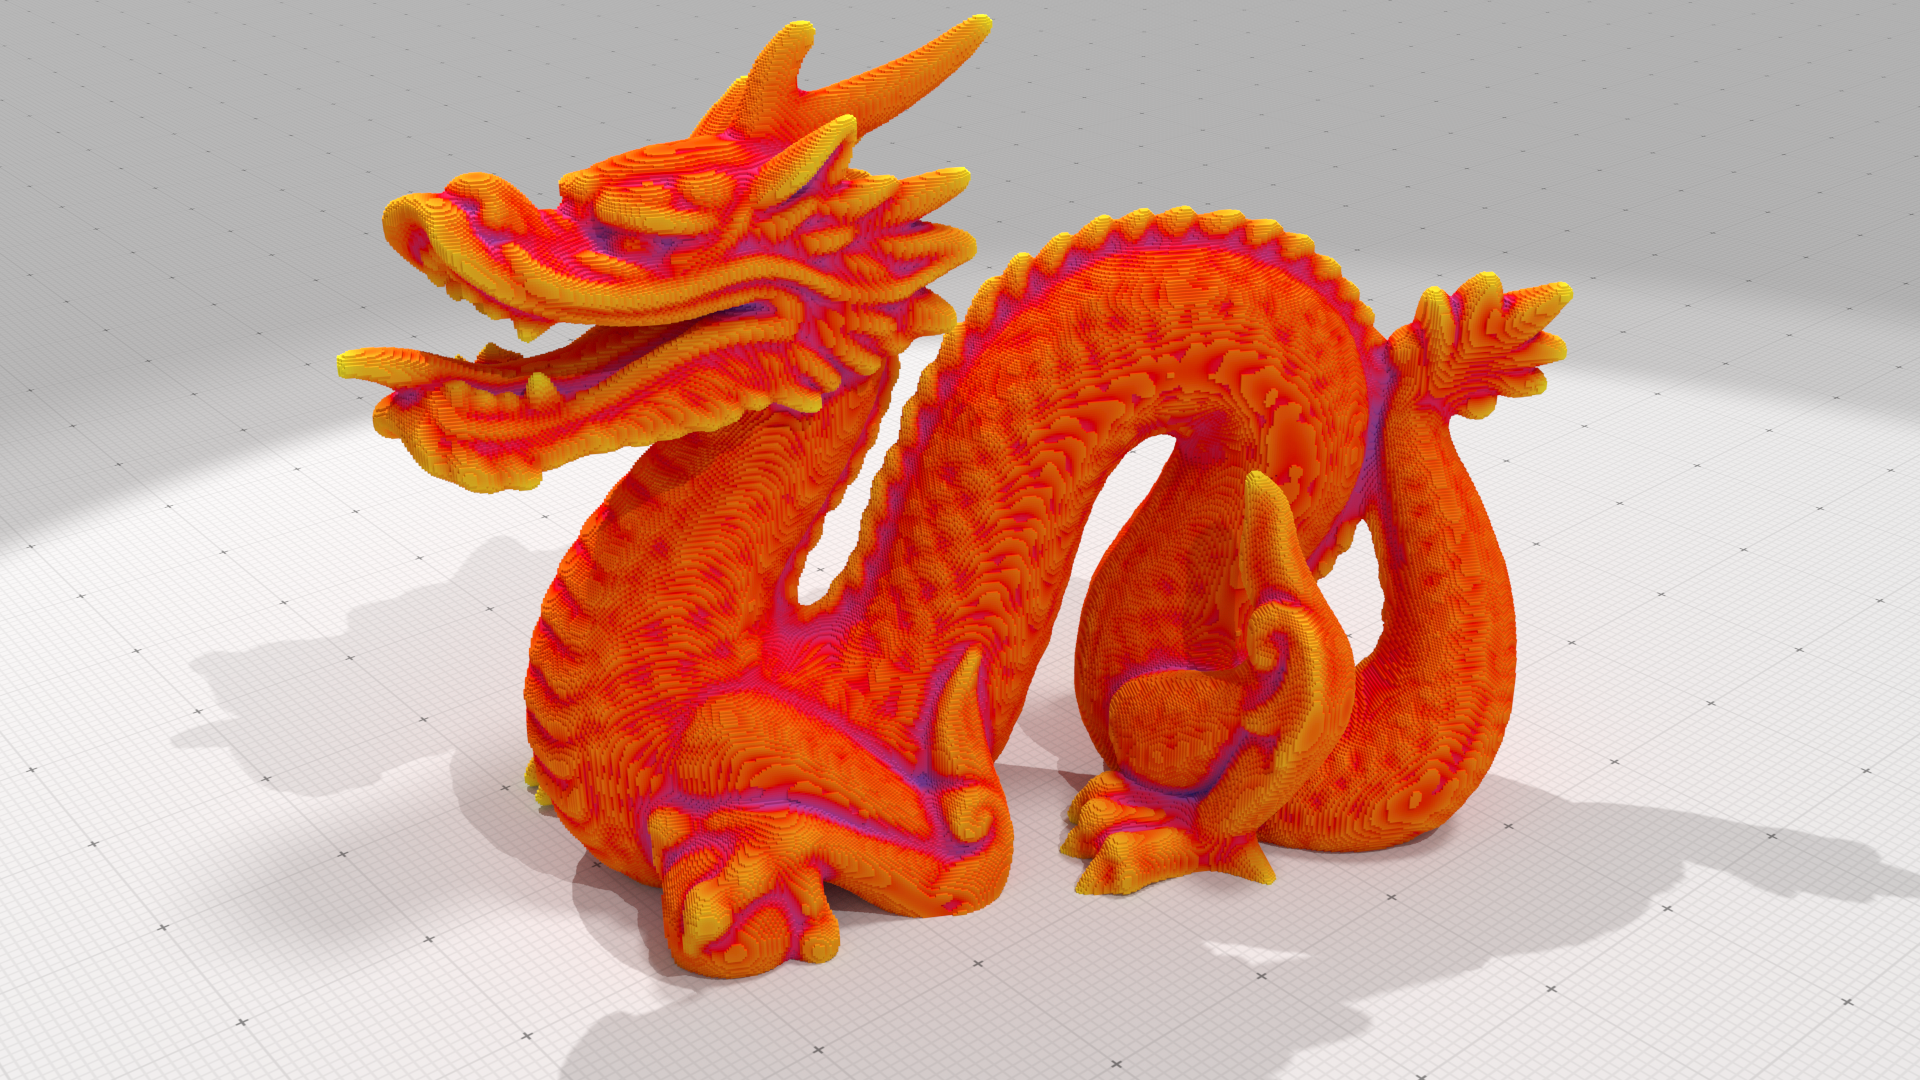
\includegraphics[width=10cm]{images/Teaser}


        %\myDegree \\
        %\myDepartment \\
        %\myFaculty \\
        %\myUni \\ \bigskip

        %\myTime\ -- \myVersion

				%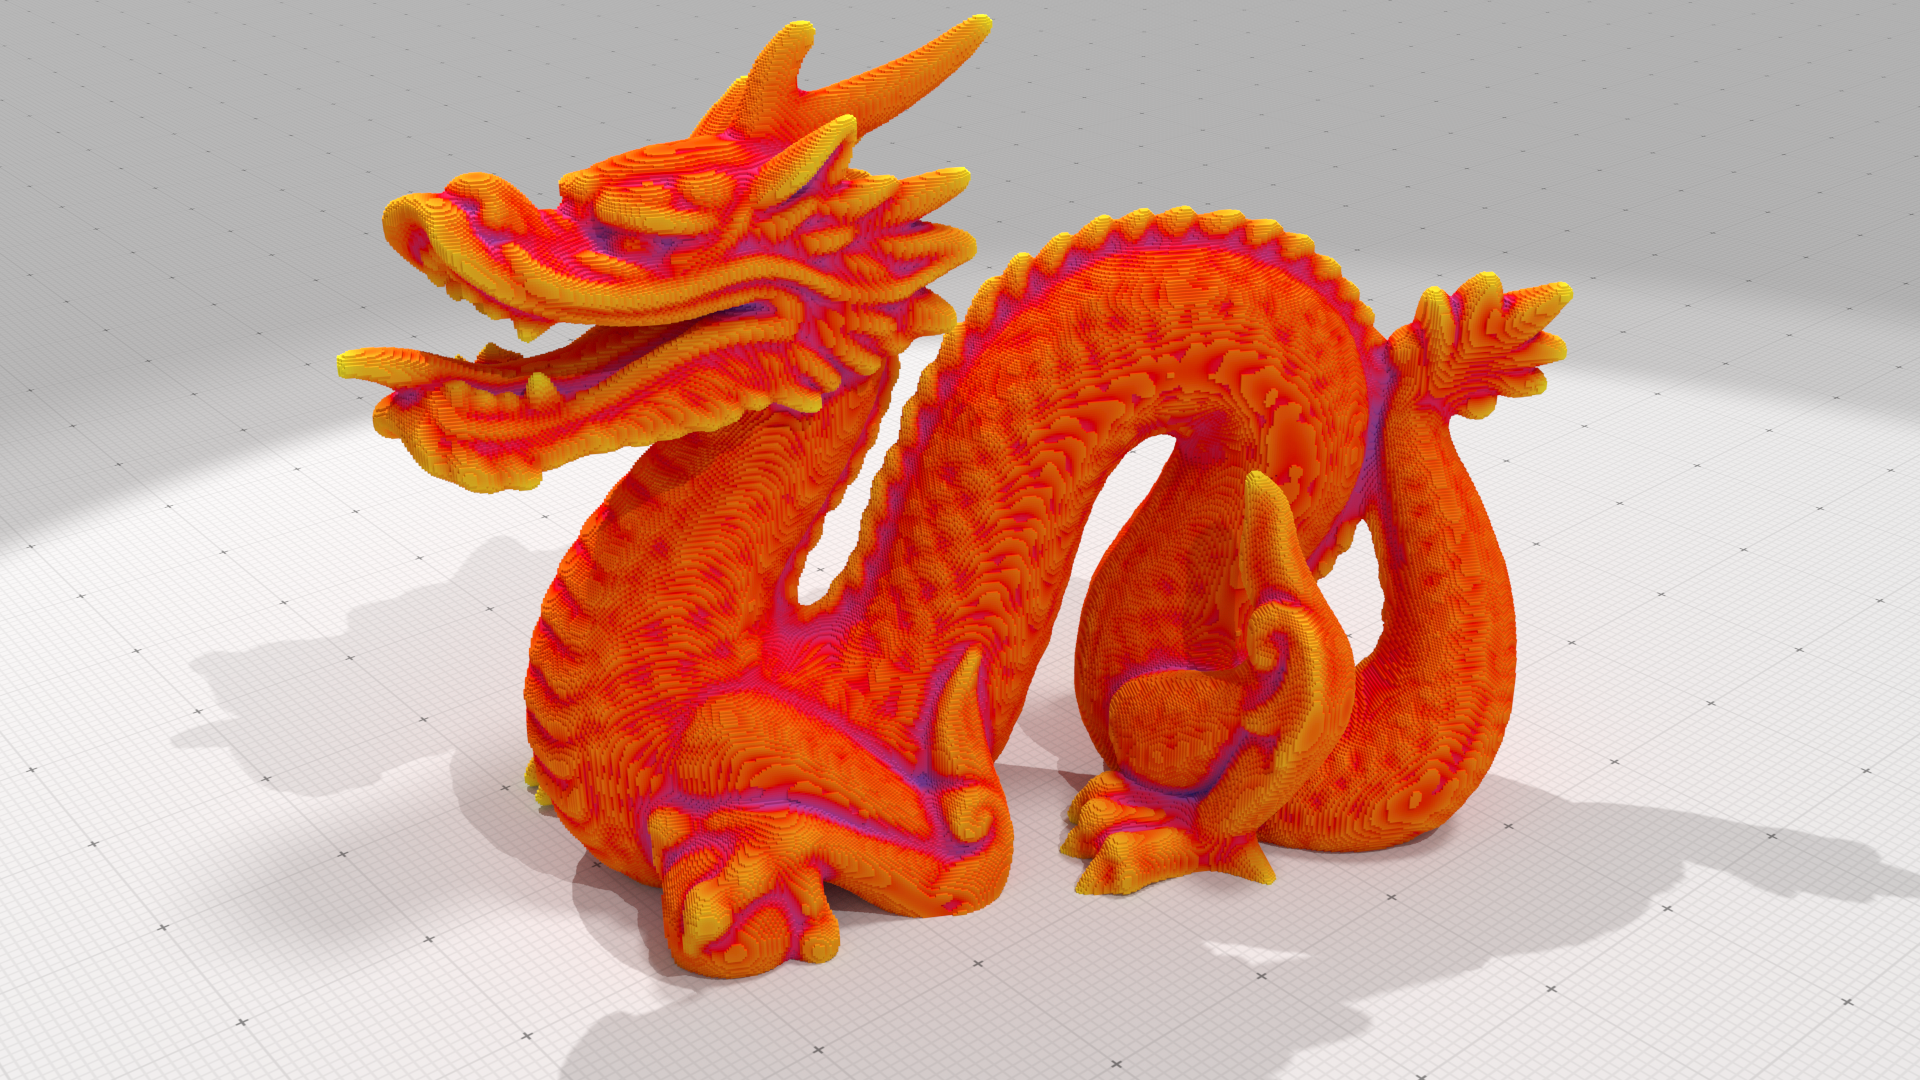
\includegraphics[width=10cm]{images/Teaser} \\ \medskip

        \vfill

        \textbf{\textsc{Composition du jury}}\\ \medskip

        \begin{table}[h]
	\begin{tabular}{@{}lllr@{}}
	\hline
	M. & Pierre Alliez  & Rapporteur  & (Directeur de Recherche INRIA) \\
	M. & Éric Andrès 	  & Rapporteur  & (Professeur) \\
	M. & Yan Gérard     & Examinateur & (Maître de Conférence) \\
	M. & Simon Masnou   & Examinateur & (Professeur) \\
	M. & Nicolas Passat & Examinateur & (Professeur) \\
	M. & \thesisFirstSupervisor & Directeur de thèse & (Directeur de Recherche CNRS) \\
	M. & \thesisSecondSupervisor & Directeur de thèse & (Professeur) \\
	\end{tabular}
	\end{table}

	{
	
\includegraphics[height=1cm]{gfx/Logo_ANR}
	
\includegraphics[height=1cm]{gfx/Logo_INSALyon}
	% 
\includegraphics[height=1.2cm]{template/gfx/Logo_USMB}
	
\includegraphics[height=1cm]{gfx/Logo_LIRIS}
	
\includegraphics[height=1.5cm]{gfx/Logo_LAMA}
	}

    \end{center}
  \end{addmargin}
\end{titlepage}
		% INCLUDE: all titlepages
\begin{figure*}[htbp]
    % \centering
    \hspace*{-2cm}
    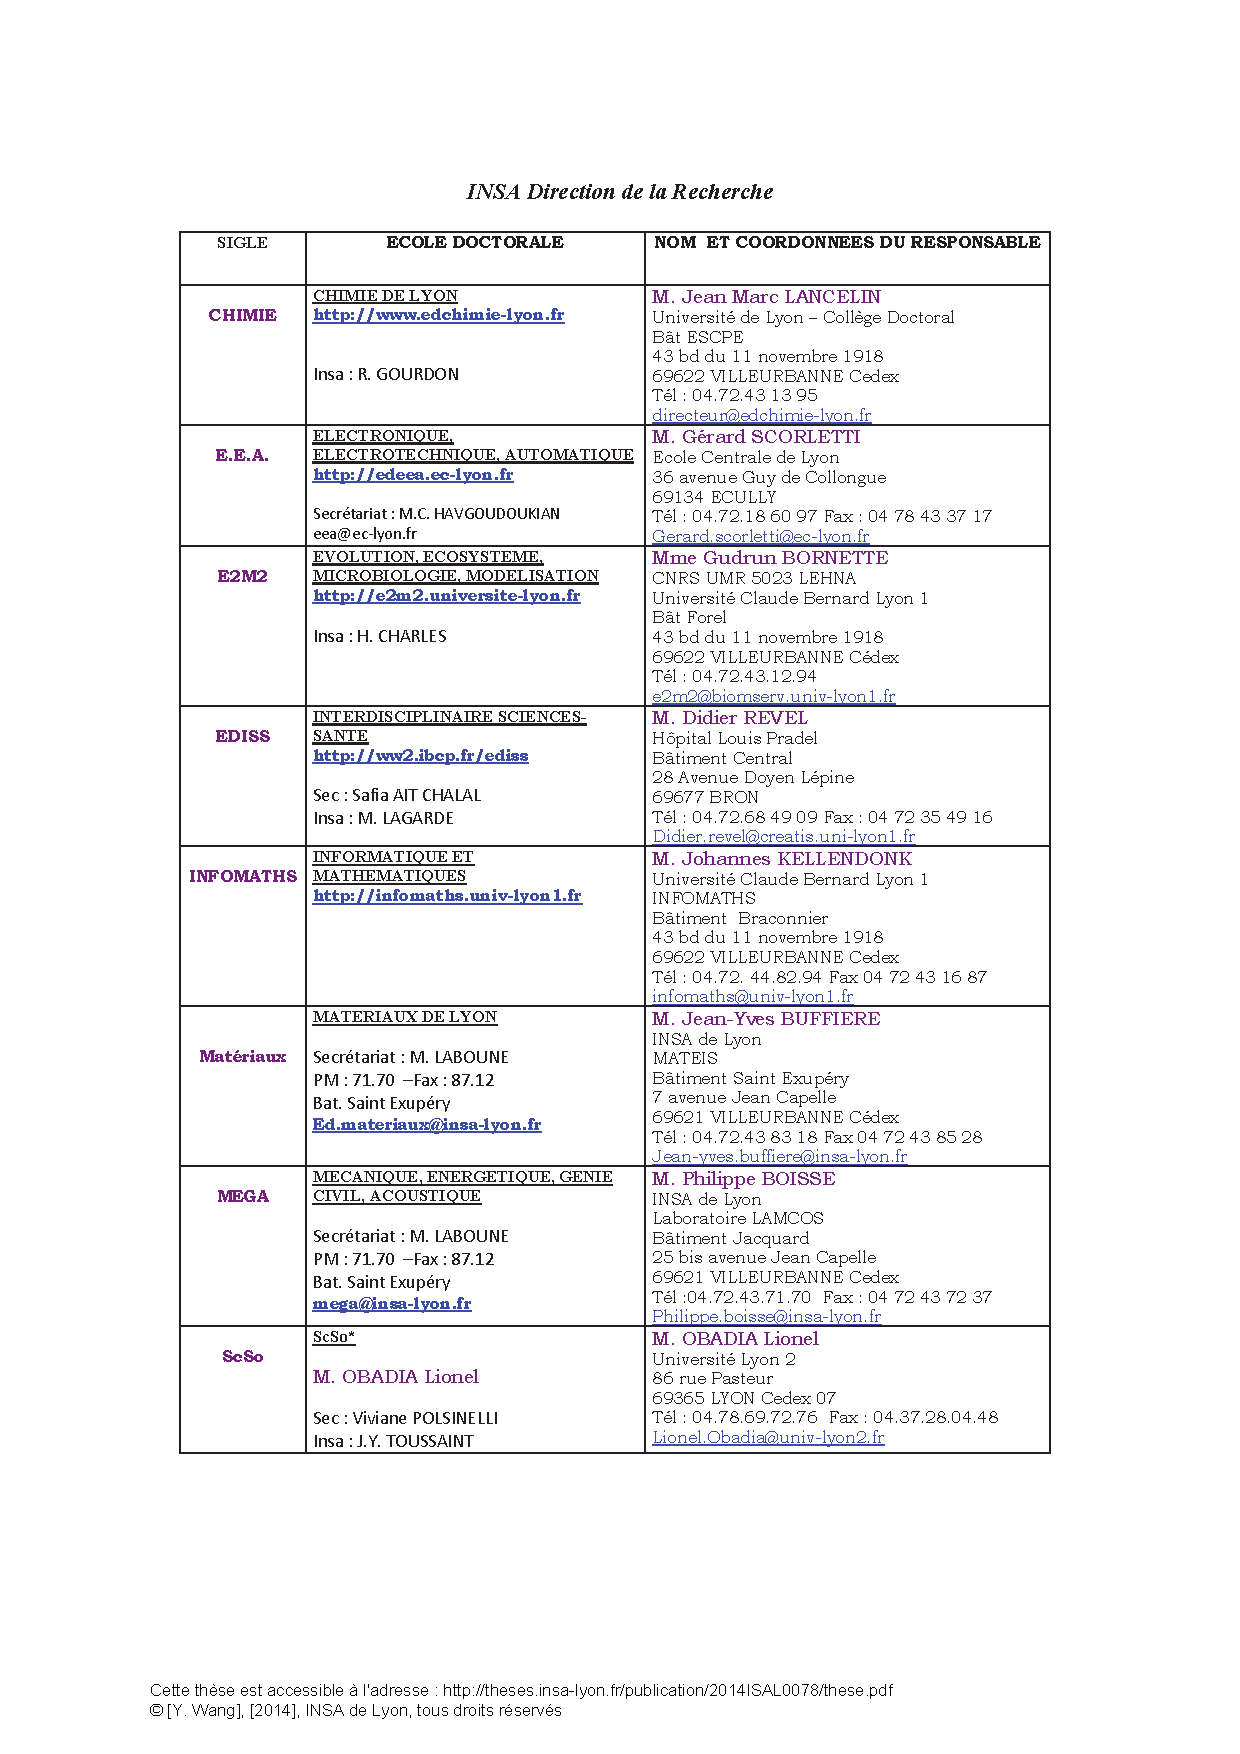
\includegraphics[trim=0cm 0cm 0cm 2.8cm, clip, width=1.30\textwidth]{gfx/ED.pdf} %% UGLY HACK because I don't want to rewrite by hand this unaesthetic document : http://www.insa-lyon.fr/sites/www.insa-lyon.fr/files/ecoles-doctorales_2011-2015_maj12102015.pdf
\end{figure*}

\clearpage

%% Folio administratif : http://www.insa-lyon.fr/sites/www.insa-lyon.fr/files/folio.doc

\includegraphics[height=1.5cm]{gfx/Logo_INSALyon}

{
\begin{center}
  \textsc{Folio administratif}\\
  \textsc{Thèse soutenue devant l'Institut National des Sciences Appliquées de Lyon}
\end{center}
}
\vfill

{
\setlength{\tabcolsep}{0pt}
\newenvironment{entrylist}{%
  \begin{tabular*}{\textwidth}{@{}p{.5\textwidth}l@{}}
}{%
  \end{tabular*}
}
% \renewcommand{\bfseries}{\headingfont\color{headercolor}}
\newcommand{\entry}[2]{%
  #1 & #2%
  \\}
\newcommand{\entryMerged}[1]{%
  \multicolumn{2}{p{\textwidth}}{#1}%
  \\}
\newcommand{\entryEmpty}[0]{%
  &%
  \\}

\begin{entrylist}
  \entry
    {\textsc{Nom :} Levallois}
    {\textsc{Date de Soutenance :} 12/11/2015 }
  \entry
    {\textsc{Prénoms :} Jérémy, Nicolas}
    {}
  \entryEmpty
  \entryMerged
    {\textsc{Titre :} Estimateurs différentiels en géométrie discrète : applications à l'analyse de surfaces digitales}
  \entryEmpty
  \entry
    {\textsc{Nature :} Doctorat}
    {\textsc{Numéro d'ordre :} \thesisOrderNumber}
  \entryMerged
    {\textsc{École Doctorale :} InfoMaths ED 512}
  \entryMerged
    {\textsc{Spécialité :} Informatique}
  \entryEmpty
  \entryMerged
    {\textsc{Résumé :} voir page \pageref{sec:abstract-french}}
  \entryMerged
    {\textsc{Mots-clés :} \emph{géométrie discrète; convergence asymptotique; quantités differentielles; courbure; normales; estimateurs; invariants par intégration; points caractéristiques; classification de surface;}}
  \entryEmpty
  \entryMerged
    {\textsc{Laboratoire(s) de recherche :} LIRIS, LAMA}
  \entryMerged
    {\textsc{Directeur(s) de thèse :} \thesisFirstSupervisor, \thesisSecondSupervisor}
  \entryMerged
    {\textsc{Président de jury :} Nicolas Passat}
  \entryMerged
    {\textsc{Composition du jury :}}
  \entry
    {Nicolas Passat}
    {Président du jury}
  \entry
    {Pierre Alliez}
    {Rapporteur}
  \entry
    {Éric Andrès}
    {Rapporteur}
  \entry
    {Yan Gérard}
    {Examinateur}
  \entry
    {Simon Masnou}
    {Examinateur}
  \entry
    {\thesisFirstSupervisor}
    {Directeur de thèse}
  \entry
    {\thesisSecondSupervisor}
    {Directeur de thèse}
\end{entrylist}
}

\vfill
 			% INCLUDE: Ecole Doctorale page
\cleardoublepage

\pagestyle{plain}			% display just page numbers
% !TEX root = ../main.tex
%
% Copyright 2015
% Jérémy Levallois <jeremy.levallois@gmail.com>
%
% This file and related figures are under Creative Commons CC BY-NC-SA 4.0
% See <https://creativecommons.org/licenses/by-nc-sa/4.0/>
%
\pdfbookmark[0]{Résumé}{Résumé}
\selectlanguage{english}
\chapter*{Abstract}
\label{sec:abstract}
\vspace*{-10mm}

3D image acquisition devices are now ubiquitous in many domains of science,
including biomedical imaging, material science, or manufacturing. Most of these
devices (MRI, Backscatter X-ray, micro-tomography, confocal microscopy, PET scans)
produce a set of data organized on a regular grid, which we call digital data,
commonly called pixels in 2D images and voxels in 3D images. Properly processed,
these data approach the geometry of imaged shapes, like organs in biomedical
imagery or objects in engineering.

In this thesis, we are interested in extracting the geometry of such digital
data, and, more precisely, we focus on approaching geometrical differential
quantities such as the curvature of these objects. These quantities are the
critical ingredients of several applications like surface reconstruction or
object recognition, matching or comparison. We focus on the proof of multigrid
convergence of these estimators, which in turn guarantees the quality of
estimations. More precisely, when the resolution of the acquisition device is
increased, our geometric estimates are more accurate. Our method is based on
integral invariants and on digital approximation of volumetric integrals.

Finally, we present a surface classification method, which analyzes digital data
in a multiscale framework and classifies surface elements into three categories:
smooth part, planar part, and singular part (tangent discontinuity). Such
feature detection is used in several geometry pipelines, like mesh compression
or object recognition. The stability to parameters and the robustness to noise
are evaluated with respect to state-of-the-art methods. All our tools for
analyzing digital data are applied to 3D X-ray tomography of snow
microstructures and their relevance is evaluated and discussed.

% \vspace*{20mm}
\clearpage

\selectlanguage{french}
\vspace*{22mm}
{\usekomafont{chapter}Résumé}
% \chapter*{Résumé}
\label{sec:abstract-french}
\vspace*{5mm}

Les appareils d'acquisition d'image 3D sont désormais omniprésents dans
plusieurs domaines scientifiques comme l'imagerie biomédicale, la science des
matériaux ou encore l'industrie. La plupart de ces appareils (IRM, scanners à
rayons X, micro-tomographes, microscopes confocaux, TEP scans) produisent un
ensemble de données organisées sur une grille régulière que nous nommerons des
données digitales, ou plus couramment des pixels sur des images 2D et des voxels
sur des images 3D. Lorsqu'elles sont récupérées le plus justement, ces données
approchent la géométrie de la forme capturée (comme des organes en imagerie
biomédicale ou des objets dans l'ingénierie).

Dans cette thèse, nous nous sommes intéressés à l'extraction de la géométrie sur
ces données digitales. Plus précisément, nous nous concentrons à approcher des
quantités géométriques différentielles comme la courbure sur ces objets. Ces
quantités sont les ingrédients critiques de plusieurs applications comme la
reconstruction de surface ou la reconnaissance, la correspondance ou la
comparaison d'objets. Nous nous focalisons également sur les preuves de
convergence asymptotique de ces estimateurs, garantissant en quelque sorte la
qualité de l'estimation. En effet, lorsque la résolution de l'appareil
d'acquisition est augmentée, notre estimation géométrique est plus précise.
Notre méthode est basée sur les invariants par intégration et sur
l'approximation digitale des intégrations volumiques.

Enfin, nous présentons une méthode de classification de la surface, qui analyse
les données digitales dans un système à plusieurs échelles et classifie les
éléments de surface en trois catégories : les parties lisses, les parties
planes, et les parties singulières (discontinuités de la tangente). Ce type de
détection de points caractéristiques est utilisé dans plusieurs algorithmes
géométriques, comme la compression de maillage ou la reconnaissance d'objet. La
stabilité aux paramètres et la robustesse au bruit sont évaluées en fonction des
méthodes de la littérature. Tous nos outils pour l'analyse de données digitales
sont appliqués à des micro-structures de neige provenant d'un tomographe à
rayons X, et leur intérêt est évalué et discuté.
		% INCLUDE: the abstracts (english and french)
\cleardoublepage

% !TEX root = ../thesis-example.tex
%
\pdfbookmark[0]{Acknowledgement}{Acknowledgement}
\chapter*{Acknowledgement}
\label{sec:acknowledgement}
\vspace*{-10mm}

% \Blindtext[2][2]
      % INCLUDE: Annexe
\cleardoublepage

\pdfbookmark[0]{Remerciements}{Remerciements}
\chapter*{Remerciements}
\label{sec:remerciements}
\vspace*{-10mm}

\cleanchapterquote{
%
Just do it.\\
Make your dreams come true.\\
Nothing is impossible.\\
Yes you can.
%
}{Shia \textsc{LaBeouf}}{}

C'est marrant, au début de ma thèse, le moment où j'allais rédiger cette page
des remerciements me paraissait tellement loin. Et maintenant, j'en suis à cette
étape. C'est marrant.

Et si j'en suis à écrire ces mots, c'est en grande partie grâce à David \textsc{Coeurjolly} et
Jacques-Olivier \textsc{Lachaud}, « \emph{papa} et \emph{maman} »\footnote{Personne ne sait qui
est le \emph{papa} et qui est la \emph{maman}.}, qui m'ont fait confiance et
m'ont soutenu, surtout dans les moments de doute, tout au long de cette thèse.
C'était un vrai plaisir de travailler avec vous, de discuter avec vous. J'ai
énormément appris grâce à vous et je vous en suis très reconnaissant.

Je remercie les membres de mon jury, Nicolas \textsc{Passat}, Pierre
\textsc{Alliez}, Éric \textsc{Andrès}, Yan \textsc{Gérard}, Simon
\textsc{Masnou} pour voir répondu sans hésitation favorablement à l'évaluation
de mon travail et pour leurs retours.

L'ambiance au travail est primordiale. À ce titre, je remercie \emph{énormément}
les membres du LIRIS-1 -- Elsa, Abdoulaye, François, Grégoire, Jean-David,
Gérémy, Matthieu --\footnote{Élu meilleur bureau de doctorants trois années
consécutives par un panel non représentatif.}. Je ne pourrais pas énumérer la
liste des choses qui se sont produites dans ce bureau lors de moments de «
craquages » tellement la liste est longue (voir la
\RefFigure{fig:jerem-in-the-truck}), allant des combats de NERF aux blind tests
d'OST de jeux vidéos, en passant par les sessions d'EuroTruck Simulator 2 avec
Oculus Rift et volant. Je ne pense pas qu'on puisse faire de meilleure ambiance
au travail que celle-ci. Merci.
%
\begin{figure}[ht]{
  \begin{center}
    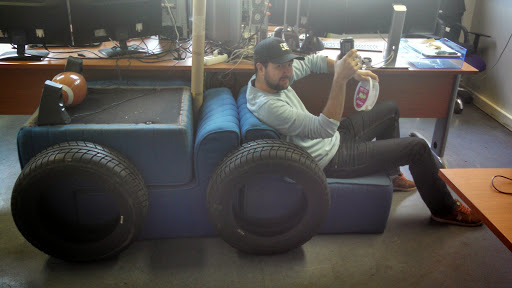
\includegraphics[width=8cm]{images/misc/JeremInTheTruck}
  \end{center}
  \caption{Reproduction à l'échelle $1:10$ d'un camion avec le mobilier à disposition.\label{fig:jerem-in-the-truck}}}
\end{figure}

Merci également aux « amis du LIRIS-1 », contribuant à l'esprit LIRIS-1 --
Hélène, Karolina, Lucille, Marie-Neige, Rubiela, Joseph --. Ces (\emph{un peu
moins de}) quatre années de thèse ont été un vrai plaisir en votre compagnie.
Parce qu'il n'y a pas que le travail dans la vie, ces années de thèses ont été
sublimés (tel un gâteau dans Top Chef) grâce à vous par quelques sorties «
extra-scolaires » : journées au ski, laser game, course à pied, VTT et j'en
passe. C'était vraiment cool et parfois ça fait du bien de se vider la tête.

Je ne remercie pas la SNCF, pour avoir rendu mes trajets à Chambéry de
véritables calvaires à coups de « Perte d'adhérence sur les rails » ou de «
Raté d'ouverture d'un passage à niveau ».

Un grand merci aux secrétaires du LIRIS et du LAMA, surtout à Sylvie qui m'a
débloqué pas mal de situations dont un fameux appel, un lundi matin : «
Euh ... je crois que j'ai raté mon avion. Je fais quoi ? ».

Merci également à mes collègues au sein des équipes m2DisCo et LIMD, et plus
largement au LIRIS et au LAMA, ainsi que de l'ANR digitalSnow pour ces
discussions riches autour de domaines variés.

J'ai une pensée pour Yoann \textsc{Pigné} -- à l'époque doctorant à l'Université
du Havre lors de ma première année de Licence -- qui, sans le savoir, m'a donné
envie de faire une thèse.

Une pensée également au club des \emph{gentlemen}, « Les Barons », -- Mierre,
Dhomas, Grançois, TFC -- dont les nombreuses soirées « Rétro-bièring » et les
discussions autour des jeux vidéos, de l'informatique ou des sciences en général
ont été une source inépuisable d'échange de connaissance. Je ramène un jeu NES
de ma collection pour la prochaine soirée.

Je suis extrêmement redevable envers mes « conseillers personnels » -- Dav,
\barre{Léa} Zouille, JD, L0ur5, Sandrine -- qui ont su m'aiguiller lors des
moments de doute.

Un petit mot aussi à Marion et Thomas, doctorants avec lesquels je partage au
moins un encadrant. Je vous souhaite bon courage pour la suite de votre thèse.
Vous verrez, la soutenance arrive vite !

Enfin, et non des moindre, je voudrais remercier mes parents et mes soeurs qui
n'ont eu de cesse de me soutenir, même s'ils ne comprenaient pas vraiment ce que
je faisais. Je remercie bien évidemment Audrey pour m'avoir épaulé chaque jour.

Avant de vous laisser lire le contenu plus \emph{scientifique} (ou bien me
rédiger un mail d'insulte parce que je vous ai oublié dans ces
remerciements\footnote{Si c'est le cas, les sources de ma thèse sont disponibles
sur GitHub : \url{https://github.com/jlevallois/PhD-Thesis}, faites un
pull-request pour vous rajouter.}), je voudrais revenir sur les citations en
début de chapitre. Ne cherchez pas de cohérence avec le contenu des chapitres,
celles-ci ont été choisies car elles représentent quelque chose qui a été
important pour moi (un livre, un film, une série). C'est pour moi, en quelque
sorte, un moyen de remercier l'auteur.
 		% INCLUDE: remerciements
\cleardoublepage


\setcounter{tocdepth}{2}		% define depth of toc
\tableofcontents						% display table of contents
\cleardoublepage

% \listoftodos
% \cleardoublepage

% --------------------------
% Body matter
% --------------------------

\pagenumbering{arabic}							% arabic page numbering
\setcounter{page}{1}								% set page counter
\setcounter{secnumdepth}{3}					% set counter to 3 depth (subsubsection)
\pagestyle{maincontentstyle}				% fancy header and footer
\mtcsettitle{minitoc}{Sommaire}
%
% !TEX root = ../main.tex
%
% Copyright 2015
% Jérémy Levallois <jeremy.levallois@gmail.com>
%
% This file and related figures are under Creative Commons CC BY-NC-SA 4.0
% See <https://creativecommons.org/licenses/by-nc-sa/4.0/>
%
\chapter{Introduction et contexte -- Géométrie digitale et projet digitalSnow}
\label{sec:introduction}

\cleanchapterquote{With my freeze ray\\
I will stop the world.}{Neil Patrick \textsc{Harris} (\emph{Dr. \textsc{Horrible}})}{Dr. Horrible's Sing-Along Blog.}

\setcounter{minitocdepth}{3}
\minitoc

\newpage

Depuis quelques années, nous vivons dans un monde entouré en permanence de
\colorize{données numériques}. Il ne passe pas un jour sans que nous ne soyons
bombardés de pixels, que ce soit sur les téléphones portables, les écrans
publicitaires animés, ou peut-être même actuellement si vous lisez ce document
sur un écran. Devant cette masse grandissante de pixels, ou de voxels en
dimension 3, les besoins en traitement de ces données digitales sont de plus en
plus forts. Dans l'imagerie médicale par exemple, nous sommes capables de
récupérer de manière non-invasive un « amas de voxels » représentant un organe
d'un patient. Il existe une demande de plus en plus forte également pour la
sauvegarde du patrimoine culturel : les œuvres ont une durée de vie limitée par
le choix de leurs matériaux ou à cause d’événements extérieurs (guerres,
catastrophes naturelles); il devient alors préoccupant de les stocker
numériquement.

Le cadre de cette thèse, avec le \colorize{projet \digitalSnow}, est d'étudier
les métamorphoses de neige difficilement observables à l'œil nu grâce à leur
représentation digitale. Le projet \digitalSnow\footnote{ANR-11-BS02-009,
\url{http://liris.cnrs.fr/dsnow/}} est un projet de recherche financé par
l'Agence Nationale de le Recherche qui regroupe trois laboratoires spécialisé
dans des domaines différents : le laboratoire d'informatique
\textsc{\colorize{LIRIS}} de l'Université de Lyon, le laboratoire de
mathématiques \textsc{\colorize{LAMA}} de l'Université de Savoie Mont-Blanc, et
le Centre d'Études de la Neige \textsc{\colorize{CEN}} du Centre National de
Recherches Météorologiques. Lors d'une chute de neige, les cristaux de glace
s'accumulent sur le sol et forment un ensemble poreux d'air humide, de glace et
d'eau. Cette neige se transforme avec le temps; l'enjeu ici est de comprendre
comment évolue la micro-structure de la neige en fonction des conditions
extérieures et des phénomènes intrinsèques du matériau (tension de surface). Pour
ce faire, nous récupérons des images digitales de dimension 3 de
micro-échantillons de neige grâce à la micro-tomographie à rayons X et nous
cherchons à extraire des quantités topologiques et géométriques (comme la
courbure) afin de modéliser les propriétés physiques du matériau. Nous
préciserons le contexte applicatif dans le
\RefSection{sec:applications:digitalsnow}.

La \colorize{\DigitalGeometry} tente alors d'apporter des outils mathématiques
permettant d'exploiter pleinement ces données digitales. Ces outils proviennent
généralement de la géométrie euclidienne classique et sont adaptés pour des
données digitales (parties de $\Z^d$). Cependant, comme le dit Jean
\textsc{Françon} dans la préface de « Géométrie discrète et images numériques »
\cite{Coeurjolly2007Book}, la \DigitalGeometry n'est pas seulement l'étude
d'objets du monde réel dans l'espace digital, mais également l'étude de l'objet
digital lui-même. Ainsi, sous l'impulsion de Jean-Pierre \textsc{Reveillès} dès
1988, la géométrie arithmétique s'intéresse aux droites et cercles non plus
comme étant seulement le produit d’un algorithme de tracé mais définis
intrinsèquement dans la géométrie digitale, sans l’être par approximation du
continu.

La principale motivation est d'approcher au plus près la représentation digitale
de l'objet de sa version euclidienne. Ainsi nous nous intéressons aux questions
suivantes : comment récupérer des informations sur l'objet réel étudié lorsque
nous n'avons à notre disposition qu'une version approchée de celui-ci, sa
version discrétisée ? Pouvons-nous garantir la qualité des quantités estimées
sur les données digitales ? Après de rapides définitions des notions et outils
de base utilisés en géométrie digitale dans le \RefChapitre{sec:notions}, nous
proposons dans le \RefChapitre{sec:estimators}, des estimateurs digitaux de
courbure en dimension 2 et 3 (courbure moyenne, courbures principales) avec des
preuves mathématiques garantissant la qualité des résultats (propriété de
convergence asymptotique uniforme). Nous adapterons ces estimateurs dans ce même
chapitre afin qu'ils ne nécessitent aucun paramètre. Ensuite, dans le
\RefChapitre{sec:applications}, nous dérivons ces estimateurs de courbure afin
de reconnaître les singularités d'un objet, en quelque sorte les arêtes de
l'objet sous-jacent à sa représentation digitale. Enfin, nous conclurons et nous
apporterons quelques perspectives résultant de ces travaux dans le
\RefChapitre{sec:conclusion}.
%
%
%
% En 2000, durant l'école d'hiver « Digital and Image Geometry » en Allemagne, une
% liste de « problèmes ouverts » en géométrie et en topologie digitale a été
% dressé \cite{Klette2000OpenProblems} afin d'orienter les recherches dans le
% domaines pour les années à venir. Depuis, dans cette liste beaucoup de réponses
% ont été apportées. Mais on y trouve par exemple le problème « Algorithmes
% d'estimation et preuves de convergence asymptotique ». Déjà à l'époque cela
% représentait un problème important pouvant faire avancer le domaine de la
% géométrie digitale.
%
% Cette transition s'est également opéré dans des domaines sensibles
%
%
% Les applications sont variés et en nombre. Dans l'imagerie
% médical, dans la sauvegarde du patrimoine culturel, dans la compréhension du
% monde vivant, il n'est pas rare de récolter et stocker des données digitales.
% Ces données brutes nécessitent des algorithmes pour les comprendre, les analyser
% et en extraire des informations pertinentes.
%
% \begin{figure}[t]
%     \begin{center}
%       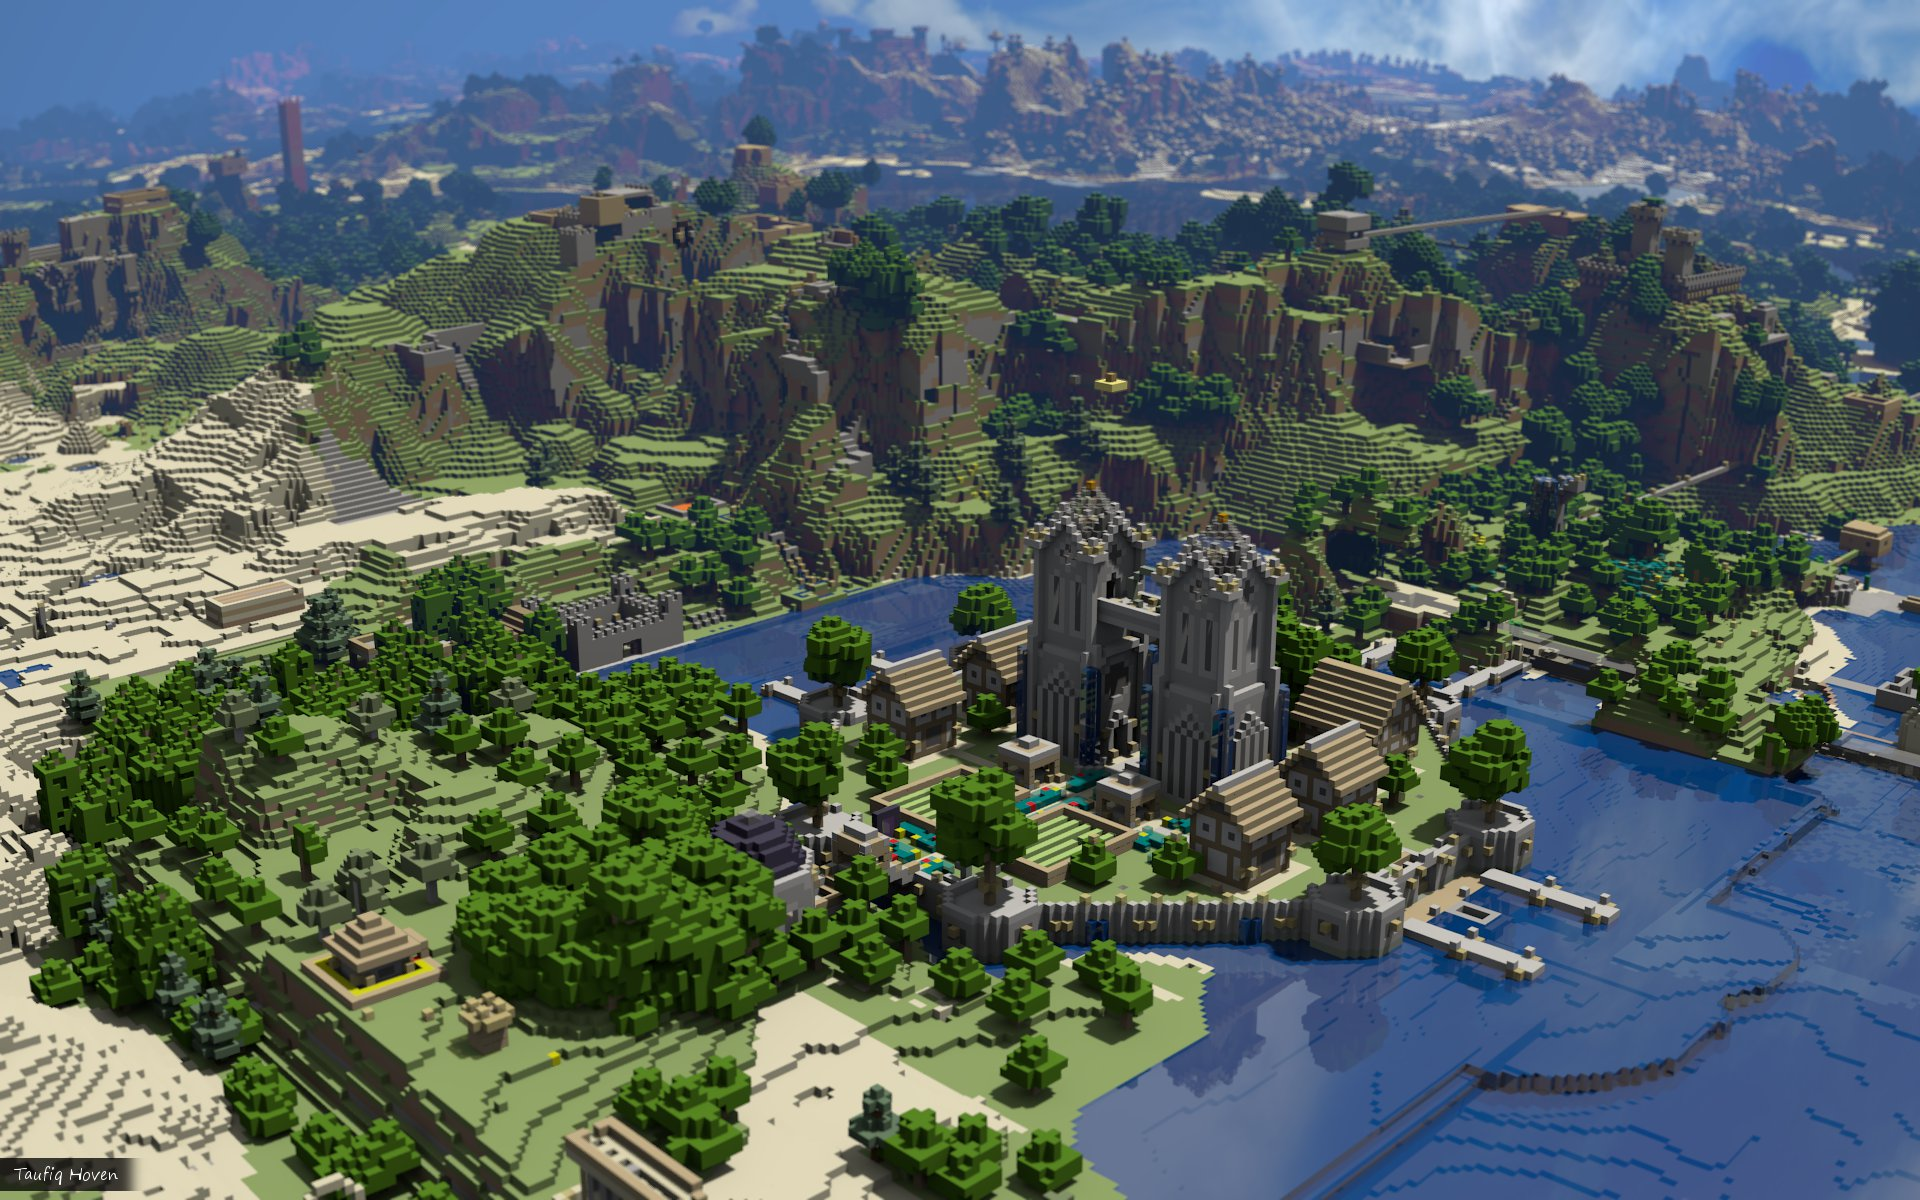
\includegraphics[width=14cm]{images/Introduction/minecraft-beautiful}
%     \end{center}
%     \caption{\textsc{Minecraft}, sorti en 2011 sur PC et plus tard sur consoles, représente un monde entièrement en voxels.}
%     \label{fig:minecraft}
% \end{figure}
%
% Un autre domaine en plein essort fait le pari des données digitales : le jeu
% vidéo. Certains moteurs de jeux ont fait le choix de basculer dans un
% environnement entièrement digital. L'exemple de jeu le plus connu est
% probablement \textsc{Minecraft}, sorti en 2011 sur PC : le joueur interagit avec
% un monde entièrement voxelique et permet de le modifier à sa guise (\RefFigure{fig:minecraft}). Un autre
% moteur comment à prendre sérieusement de l'ampleur : \textsc{Atomontage Engine}.
% Celui-ci propose de modéliser entièrement l'environnement en voxel et fait un
% post-traitement sur les données digitales afin d'avoir l'impression d'être sur
% des données continues.
%
% Ces données digitales sont l'objet de recherches intenses, même si le domaine
% reste relativement jeune.
    % INCLUDE: Introduction et Contexte -- Géométrie digitale et projet digitalSnow
% !TEX root = ../thesis-example.tex
%
\chapter{Notions et éléments de base de la géométrie digitale}
\label{sec:notions}

\cleanchapterquote{We have seen that computer programming is an art, because it applies accumulated knowledge to the world, because it requires skill and ingenuity, and especially because it produces objects of beauty.}{Jean-Claude Vandamme}{Ma vie, mon œuvre.}

\setcounter{minitocdepth}{3}
\minitoc

\newpage
%
Notations:

In the sequel, points and vectors of $\R^d$ and $\Z^d$ are written in
bold, and for some point or vector $\vz \in \Z^d$, its coordinates or
components are written with subscripts as $\vz=(z_1,\ldots,z_d)$.
%
% Introduction à la géométrie différentielle ?
%
% courbure : Defining and studying the curvatures of singular spaces goes back to Steiner (1840) in the convex case (see [30] for instance). ([30] = L. Santalo, Integral geometry anf geometric probability, Encyclopedia of Math- ematics and its applications, Vol. 1. Addison-Wesley Publishing Co. (1976), MR0433364, Zbl 0342.53049.)
%
\section{Discrétisation}
%
% Parler de discret vs digital
\section{Estimateurs locaux et globaux}
%
\section{Convergence asymptotique d'estimateurs}
% la convergence asymptotique comme un critère essentiel
% pour un estimateur \cite{Coeurjolly_ChapEstimateur}
%
\section{Introduction à la géométrie différentielle}
%
\section{Droites digitales standard, segments digitaux, arcs de cercle digitaux}%
\label{sec:segments}
%
\begin{definition}{\fakeTitle{Droite digitale standard et segment digital (« \anglais{Digital Straight Segment} ») \cite{Reveilles1991}}}
  \label{def:DSS}
%
  L'ensemble de points $(x_1,x_2) \in \Z^2$ satisfaisant $\mu \le ax_1 - bx_2 <
  \mu + |a| + |b|$, avec $a$, $b$ et $\mu$ des nombres entiers, est appelé une
  \emph{droite digitale standard} avec comme pente $a/b$ et comme décallage
  $\mu$. Tout sous ensemble de pixels connectés d'une droite digitale standard
  est un \emph{segment digital} (ou « \anglais{DSS} »).
%
\end{definition}
%
Une droite digitale standard est une droite 4-connexe.
%
\begin{definition}{\fakeTitle{Segments maximaux et faisceau de segments maximaux \cite{Lachaud2007}}}
  \label{def:MDSS}
%
  Les pointels composant le bord digital $\BdZ{\DigShape}$ d'une forme
  $\DigShape \subset \Z^2$ forme un contour $4$-connecté. Cela nous permet de
  les dénombrer consécutivement par $(\vp_i)_{i={0\ldots n-1}}$. Une séquence de
  pointels $(\vp_i, \ldots, \vp_j)$ (dont l'indice est modulo $n$) est un
  \emph{segment maximal} (ou « \anglais{MDSS} ») sur $\BdZ{\DigShape}$ si c'est
  un DSS qui ne peut s'étendre dans aucun sens (en avant ou en arrière) en
  restant un DSS.
  %
  \\
  %
  Plus formellement, $(\vp_i, \ldots, \vp_j)$ est un segment maximal sur $\BdZ{\DigShape}$ \ssi :
  \begin{itemize}
    \item $(\vp_i, \ldots, \vp_j)$ est un DSS sur $\BdZ{\DigShape}$,
    \item $(\vp_{i-1}, \ldots, \vp_j)$ n'est pas un DSS sur $\BdZ{\DigShape}$,
    \item $(\vp_i, \ldots, \vp_{j+1})$ n'est pas un DSS sur $\BdZ{\DigShape}$,
  \end{itemize}
  %
  Pour un pointel $\vp \in \BdZ{\DigShape}$ donné, le \emph{faisceau de segments maximaux} à $\vp$ est l'ensemble
  des segments maximaux de $\BdZ{\DigShape}$ contenant $\vp$.
%
\end{definition}
%
\cauthors{Lachaud}{lachaud2006HDR} et \cauthors{de
Vieilleville}{deVieilleville2007} se sont intéressés sur les propriétés
asymptotiques des longueurs des segments maximaux sur des formes convexe
suffisamment lisse de dimension 2 :
%
\begin{lemma}{\fakeTitle{Lois asymptotiques des segments maximaux}}
  \label{lem:law-length-MDSS}
  %
  Soit $\Shape$ une forme convexe de $\R^2$, avec un bord $C^3$ à
  courbure bornée non nulle. La longueur discrète des segments maximaux de
  $\BdZ{\DigShape}$ pour $\DigShape = \DSh$ suit les règles suivantes :
  %
  \begin{itemize}
    %
    \item le plus court des segments maximaux a une borne inférieure en
    $\Omega(h^{-\frac{1}{3}})$;
    %
    \item le plus long des segments maximaux a une borne supérieure en
    $O(h^{-\frac{1}{2}})$;
    %
    \item la longueur moyenne des segments maximaux $L_D({\DigShape})$, est bornée par :
    %
    \begin{equation}
      \label{eq:lengthMS}
      \Theta(h^{-\frac{1}{3}}) \le L_D( {\DigShape} ) \le \Theta(h^{-\frac{1}{3}} \log \left(\frac{1}{h}\right))\;.
    \end{equation}
  \end{itemize}
  %
\end{lemma}
%
\begin{figure}[ht]{
    \begin{center}
    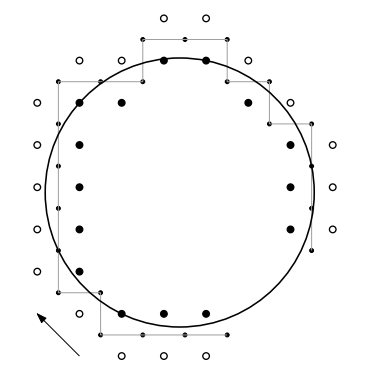
\includegraphics[height=6cm]{images/Notions/DCA}
    \end{center}}
    \caption[Arc de cercle digital.]{Arc de cercle digital (Figure~1.22 de \cite{Roussillon2009}).\label{fig:dca-figure}}
\end{figure}
%
\begin{definition}{\fakeTitle{Arcs de cercle digitaux}}
  \label{def:digital-circular-arc}
  %
  Soit $\Shape$ une forme convexe de $\R^2$, avec un champ de courbure continue.
  Le contour digital $\BdZ{\DigShape}$ pour $\DigShape = \DSh$ est un arc de
  cercle digital (\anglais{DCA}) si et seulement s'il existe un cercle euclidien
  qui sépare les points intérieurs à $\BdZ{\DigShape}$ des points digitaux extérieurs de
  $\BdZ{\DigShape}$ (voir \RefFigure{fig:dca-figure}).
  %
  \\
  %
  Un arc de cercle digital est maximal (\anglais{\MDCA}) si et seulement s'il ne
  peut être étendu dans aucune direction.
  %
\end{definition}
%
\section{Estimateurs digitaux d'aire, de volume, de moments, de positionnement de surface}
%
\subsection{Aire et volume digitaux}
%
\subsubsection{Aire et volume en comptant les points digitaux}
\label{sec:AreaByCounting}
%
Une façon simple de calculer l'aire ou le volume d'une forme digitale consiste à
compter le nombre de points digitaux appartenant à la forme. Plus formellement,
pour tout sous-ensemble $\DigShape \subset \Z^2$, l'estimateur digital d'aire au pas
de discrétisation $h$ est défini par :
%
\begin{equation}
  \AreaC(\DigShape, h) \EqDef h^2 \MCard(\DigShape)
\end{equation}
%
En dimension $3$, nous noterons l'estimateur digital de volume au pas de
discrétisation $h$ :
%
\begin{equation}
  \VolC(\DigShape, h) \EqDef h^3 \MCard(\DigShape)
\end{equation}
%
Maintenant, si ce sous-ensemble digital $\DigShape$ provient de la discrétisation de
formes euclidiennes $\Shape$, nous voulons que l'estimation du volume devienne
meilleure lorsque le pas de discrétisation $h$ se raffine (voir
\RefSection{sec:notion:multigridconvergence}). Il est connu depuis
\nauthor{Gauss} et \nauthor{Dirichlet} que cette façon d'estimer l'aire donne
des résultats de convergence asymptotique sur les formes $\Shape$ convexes
finies de $\R^2$ :
%
\begin{equation}
  \label{eq:AreaByCountingConv}
  \AreaC(\DigF{\Shape}{h},h) = \Area(\Shape) + O(h^\beta),
\end{equation}
%
avec $\beta = 1$ dans le cas général \cite{Klette2000}, et peut être optimisé à
$\beta = \frac{15}{11} - \epsilon$ avec $\epsilon > 0$ (arbitrairement petit)
lorsque le bord de l'objet est $C^3$ à courbure non nulle \cite{Huxley1990}.
De mêmes résultats ont été proposés en 3D :
%
\begin{equation}
  \label{eq:VolumeByCountingConv}
  \VolC(\DigF{\Shape}{h},h) = \Vol(\Shape) + O(h^\gamma),
\end{equation}
%
avec $\gamma = 1$ dans le cas général \cite{Kratzel1988}, et peut être amélioré à
$\gamma=\frac{243}{158}$ lorsque le bord est lisse \cite{Guo2010}.
%
En dimension 2, les objets non convexes suivent les mêmes règles tant que
$\Shape$ peut être exprimé comme une somme ou une différence de régions convexes
bornées par des courbes fermées simples \cite{Huxley1996}. Ces résultats
précédents restent valides chaque fois que le bord de la forme peut être
décomposé en nombre fini de morceaux convexes (ou convexe $C^3$ à courbure non
nulle pour les bornes améliorées).
%
\subsection{Moments géométriques digitaux}
%
Le concept mathématique des moments a beaucoup été étudié depuis plusieurs
années et trouve son champ d'application sans cesse augmenté, allant des
statistiques et mécaniques (\anglais{General moment theory}) \cite{} à la
reconnaissance de formes (\cauthors{Trier}{Trier1996} pour un survey sur la
reconnaissance de caractères, \cite{}) et la reconstruction d'objets \cite{Ghorbel2005}.
La première utilisation des moments en analyse d'images remonte à 1962 par
\cauthor{Hu}{Hu1962} pour la reconnaissance de caractères.
%
Les moments ont l'avantage d'être indépendant à l'échelle, la position et
l'orientation, en faisant un outil invariant robuste \cite{}. Nous allons tout
d'abord définir ce que sont les moments et leurs caractéristiques, pour ensuite
nous intéresser à les estimer sur des données digitales.
%
\todoJeremy{Le papier Reconstructing With Geometric Moments \cite{Ghorbel2005} est pas mal niveau intro}
%
\subsubsection{Définition et propriétés des moments géométriques}%
\label{sec:definitions-moments}
%
Une définition générale du moment géométrique (ou moment cartésien) $\Mom{p_1
\cdots p_d}$ d'ordre $p_1 \cdots p_d$ (aussi appelé le $p_1 \cdots p_d$-moment)
de $\Shape$ (de $\R^d$) peut être donnée comme :
%
\begin{equation}
  \Mom{p_1 \cdots p_d}(\Shape) \EqDef \idotsint_{\Shape} x_1^{p_1} \cdots x_d^{p_d} f(x_1 \cdots x_d) dx_1 \ldots dx_d.
\end{equation}
%
\paragraph{Moment d'ordre zéro : aire / volume}
%
Il apparaît alors que le $0\cdots0$-moment correspond à l'aire en 2D ou au
volume en 3D de $\Shape$ :
%
\begin{equation}
  \Mom{0 \cdots 0}(\Shape) \EqDef \idotsint_{\Shape} f(x_1 \cdots x_d) dx_1 \ldots dx_d.
\end{equation}
%
\paragraph{Moments du premier ordre : barycentre}
%
Les $d$ moments du premier ordre ($\Mom{1 0 \cdots 0}(\Shape)$, $\Mom{0 1 0
\cdots 0}(\Shape)$, $\cdots$, $\Mom{0 \cdots 0 1}(\Shape)$) sont généralement
utilisés pour déterminer le barycentre de la forme à analyser. Les coordonnées
du barycentre $(\overline{x_1}, \cdots, \overline{x_p})$ sont :
%
\begin{equation}
  \overline{x_1} = \frac{\Mom{1 0 \cdots 0}(\Shape)}{\Mom{0 \cdots 0}(\Shape)}, \cdots, \overline{x_p} = \frac{\Mom{0 \cdots 0 1}(\Shape)}{\Mom{0 \cdots 0}(\Shape)}.
\end{equation}
%
\paragraph{Moments du second ordre}
%
Les moments du second ordre $\Mom{p_1 \cdots p_d}(\Shape)$ avec $p_1 + \cdots +
p_2 = 2$ sont connus comme les moments d'inertie, caractérisant la géométrie des
masses de la forme. En 2D, nous en dénombrons 3 : $\Mom{2 0}(\Shape)$, $\Mom{1
1}(\Shape)$ et $\Mom{0 2}(\Shape)$, en 3D il en existe 6 :  $\Mom{2 0
0}(\Shape)$, $\Mom{0 2 0}(\Shape)$, $\Mom{0 0 2}(\Shape)$, $\Mom{1 1
0}(\Shape)$, $\Mom{0 1 0}(\Shape)$ et $\Mom{1 0 1}(\Shape)$
%
\subsubsection{Moments en comptant les points digitaux}
\label{sec:MomentsByCounting}
%
Comme pour l'aire ou le volume précédemment, il est très simple de calculer les
moments sur des données digitales. En effet, il suffit de sommer les valeurs des
points digitaux de la forme et de remettre à l'échelle suivant le pas de
discrétisation $h$. Plus formellement, pour tout sous-ensemble $\DigShape$ de
$\Z^d$, le $p_1 \cdots p_d$-moment digital de $\DigShape$ au pas de
discrétisation $h$ est défini par :
%
\begin{equation}
  \DMom{p_1 \cdots p_d}{h}(\DigShape) \EqDef h^{d + p_1 + \cdots + p_d} \sum_{(z_1,\ldots,z_d) \in \DigShape} z_1^{p_1} \cdots z_d^{p_d} f(z_1^{p_1} \cdots z_d^{p_d}).
\end{equation}
%
Il est à noter que $f(z_1 \cdots z_d)$ est tout le temps égal à $1$ lorsque
$(z_1,\ldots,z_d) \in \DigShape$, $0$ sinon, nous pouvons alors l'enlever de
l'équation :
%
\begin{equation} \label{eq:MomentsByCounting-def}
%
  \DMom{p_1 \cdots p_d}{h}(\DigShape) \EqDef h^{d + p_1 + \cdots + p_d} \sum_{(z_1,\ldots,z_d) \in \DigShape} z_1^{p_1} \cdots z_d^{p_d}.
%
\end{equation}
%
Ainsi, le $0$-moment digital de $\DigShape$ correspond au volume digital de
$\DigShape$, \cad $\AreaC(\DigShape,h)$ lorsque $d = 2$ et $\VolC(\DigShape,h)$
lorsque $d \geq 3$.
%
Nous souhaitons alors borner l'erreur entre les moments de $\Shape$ et
l'estimation des moments digitaux de la discrétisation de $\Shape$ comme
fonction du pas de discrétisation $h$. \cauthors{Klette}{Klette2000} ont
démontré la convergence de cet estimation des moments avec une vitesse de
convergence dépendante de l'ordre du moment $\sigma = p_1 + \cdots + p_d$ :
%
\begin{equation} \label{eq:MomentsByCounting-conv}
%
  \DMom{p_1 \cdots p_d}{h}(\DigF{\Shape}{h},h) = \Mom{p_1 \cdots p_d}(\Shape) + O(h^{\mu_{\sigma}}).
%
\end{equation}
%
avec $\mu_{\sigma} \ge 1$ dans le cas général (\todoJeremy{expliciter}). Cette
borne peut être améliorer lorsque la courbure gaussienne n'est pas nulle :
\cauthors{Krätzel}{Kratzel1991} obtiennent $\mu_0=\frac{38}{25}-\epsilon$ et
\cauthors{Müller}{Muller1999} obtiennent $\mu_0 = \frac{66}{43}-\epsilon$.
\todoInlineJeremy{A verifier}
%
\section{Enveloppes convexes}
%
         % INCLUDE: Notions et éléments de base de la géométrie digitale
% !TEX root = ../main.tex
%
\chapter{Estimateurs digitaux de courbures}
\label{sec:estimators}
%
% \cleanchapterquote{We have seen that computer programming is an art, because it applies accumulated knowledge to the world, because it requires skill and ingenuity, and especially because it produces objects of beauty.}{Jean-Claude Vandamme}{Ma vie, mon œuvre.}
%
\setcounter{minitocdepth}{4}
\minitoc
%
\newpage
%
Dans ce chapitre, nous allons définir de nouveaux estimateurs de courbure pour
les surfaces digitales. Après avoir détaillé l'état de l'art
(\RefSection{sec:estimators:SOTA}), nous nous intéresserons à l'estimation de la
courbure par intégration locale (\RefSection{sec:estimators:volume}) afin d'en
extraire des estimateurs de courbure en 2D et courbure moyenne
(\RefSection{sec:estimators:volume}) et courbures principales
(\RefSection{sec:ii-3d}) en 3D. Ces estimateurs nécessitent une taille de boule
d'intégration, nous adapterons ces estimateurs à des versions ne nécessitant
aucun paramètre dans la \RefSection{sec:curvature:parameter-free}. Enfin, nous
comparerons nos estimateurs avec les méthodes représentatives de l'état de l'art
dans la \RefSection{sec:comparaison-courbure}. Dans ce chapitre, nous
considérons que $\Shapes = \Shapes^{C}$.
%
\section{Introduction}
\label{sec:estimators:introduction}
%
Comme nous l'avons vu dans le chapitre précédent (\RefSection{sec:geo-diff}), la
géométrie d'une forme est décrite à partir de ses quantités différentielles
comme la courbure.
% Et nous parlons bien de décrire, puisque toutes ces quantités sont ce
%qui la caractérise de manière unique.
C'est pour cela que plusieurs champs de recherches se tournent vers la manière
de récupérer ces quantités en les estimant à partir des
données \cite{Petitjean2002, Wang2009}.
%
%
Les données discrètes prennent différentes formes, qui sont principalement liées à la façon de capturer les
objets ou à leur utilisation. Elles peuvent être des nuages de points, des
maillages triangulés, ou encore des données digitales. Les critères guidant les définitions des
estimateurs sont différents et très liés à l'usage de la quantité différentielle :
certains privilégieront la rapidité d'estimation en dépit de la qualité notamment
dans un enjeu d'utilisation en temps interactif ou réel, tandis que d'autres (et
c'est notre cas) préféreront garantir la qualité des résultats de l'estimation
en priorité.


Comme nous l'avons vu dans le \RefChapitre{sec:introduction}, notre estimation
de la courbure est utilisée au cœur d'un processus complexe d'analyse de
déformation de microstructure de grains de neige, nécessitant des résultats les
plus justes possibles. Il nous parait également important de connaître le
comportement de l'estimateur si nous choisissons le coût d'augmenter la résolution
de la capture des données digitales : aurons-nous une meilleure estimation de la
courbure ? Nous devons alors nous focaliser sur la convergence asymptotique de
notre estimation à l'aide de preuves théoriques et de validations pratiques.
%
\section{État de l'art}%
\label{sec:estimators:SOTA}
%
\subsection{Estimation de courbure sur des maillages}
%
Les données digitales étant discrètes par nature, il semble alors pertinent de
s'intéresser aux techniques d'estimation de courbure sur des maillages
triangulés. Il existe une vaste famille de techniques en \ComputerGraphics et en
\GeometryProcessing pour estimer les courbures moyennes et gaussiennes, et
parfois même le tenseur de courbure entier. La plupart effectuent des analyses
locales (\cad limité au $1$-voisinage ou $2$-voisinage) de la forme. La
précision de l'estimation dépend fortement de la « qualité » du maillage (au
sens où ce dernier approxime suffisamment précisément la surface continue sous-jacente).

\begin{figure}[ht]
    \begin{center}
      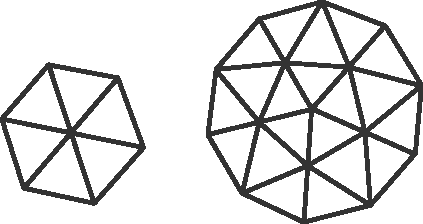
\includegraphics[width=10cm]{figures/OneRingNeighborhood}
    \end{center}
    \caption[$1$-voisinage et $2$-voisinage.]{$1$-voisinage de valence $6$ et
    $2$-voisinage de valence $5$.}
    \label{fig:one-ring-neighborhood}
\end{figure}

% Globalement, nous pouvons les distinguer en trois catégories :
% \begin{itemize}
%   \item Méthode par Correspondance
%   \item Méthodes discrètes
%   \item Estimation du tenseur de courbure
% \end{itemize}
%
\cauthors{Surazhsky}{Surazhsky2003} et \cauthors{Gatzke}{Gatzke2006} ont
proposé une étude comparative de ces estimateurs. Nous nous
référons à \cauthors{Desbrun}{Desbrun2005} et \cauthors{Bobenko}{Bobenko2008}
pour une théorie entièrement discrète. Cependant, la plupart n'ont aucunes
garanties de convergence théorique des valeurs estimées, même sans bruit sur le
maillage. Nous pouvons citer \cite{Rusinkiewicz2004} (et \cite{Page2002} pour les normales) comme
approche qui essaye de lisser les perturbations sur la surface à travers un
moyennage.
%
\paragraph{Approche par formule de Gauss-Bonnet}
%
\cauthor{Xu}{Xu2006} estime la courbure gaussienne avec une approche dérivée de
la formule de Gauss-Bonnet (défaut d'angle). Cette approche a beaucoup été
étudiée dans la littérature pour l'estimation de courbure gaussienne
\cite{Meek2000, Stokely1992} mais aussi pour de la reconstruction \cite{Dyn2001}
ou de la simplification de surface \cite{Kim2002}, et a même été déclarée « le
meilleur algorithme (NDLR: parmi 5 approches) pour l'estimation de la courbure
gaussienne » par \cauthors{Surazhsky}{Surazhsky2003}.

\begin{figure}[ht]
    \begin{center}
      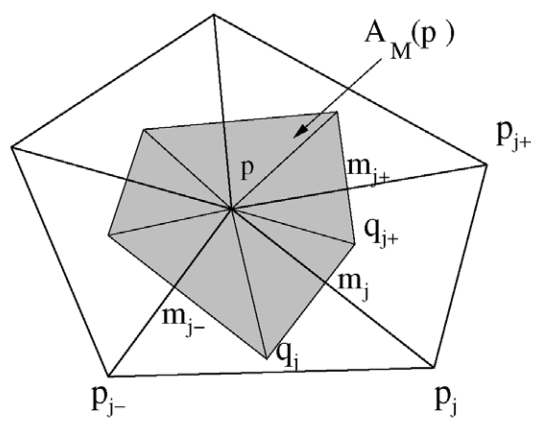
\includegraphics[width=5.5cm]{images/Curvature/Notations_Xu}
      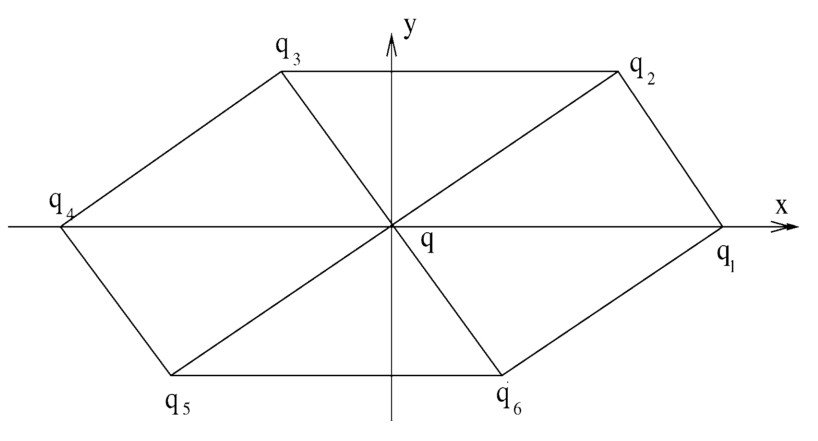
\includegraphics[width=7.5cm]{images/Curvature/Notations_Xu_2}
    \end{center}
    \caption[Notations pour \cauthor{Xu}{Xu2006}.]{\emph{À gauche :} Notations pour \cauthor{Xu}{Xu2006} (Figure~1 de \cite{Xu2006}). \emph{À droite :} Triangulation nécessaire du domaine (Figure~3 de \cite{Xu2006})}
    \label{fig:xu_notations}
\end{figure}

Soit $\vp$ un sommet de valence $6$ du maillage triangulé $M$ et $\vp_j$ avec
$j = 1,\cdots, 6$ l'ensemble des sommets du $1$-voisinage de $\vp$ (voir
\RefFigure{fig:xu_notations}-gauche pour les notations). Si $\vp$ et $\vp_j$
sont sur une surface paramétrique suffisamment lisse $F(x,y) \in \R^3$ et
qu'il existe $\vq, \vq_j \in \R^2$ tels que
(\RefFigure{fig:xu_notations}-droite, le $1$-voisinage est projeté comme des
parallélogrammes sur un plan) :
%
\begin{equation}
  \vp=F(\vq), \quad \vp_j=F(\vq_j) \quad \text{~et~} \vq_j=\vq_{j-} + \vq_{j+} - \vq \,,
\end{equation}
%
Alors, en assumant que la densité de l’échantillonnage est $\delta$ avec $A(\vp, \delta)$ la somme des aires des triangles
$[\vp\vp_j(\delta)\vp_{j+}(\delta)]$ (en gris sur la
\RefFigure{fig:xu_notations}-gauche), $\omega_j$ l'angle $\angle
\vp_j\vp\vp_{j+}$, ils démontrent que :
%
\begin{equation}
  \frac{3}{A(\vp,\delta)} \left[ 2\pi - \sum \limits^6_{j=1} \omega_j(\delta) \right] \EqDef \GaussCurv(\vp) + O(\delta^2) \,,
\end{equation}
%
quand $\delta$ tend vers $0$, où $\GaussCurv(\vp)$ est la valeurs de courbure
gaussienne au point $\vp$.
%
%
L'auteur propose une propriété de convergence supplémentaire lorsque
l'échantillonnage est perturbé par une erreur $O(\delta^\alpha)$, mais avec
$\alpha \ge 3$.


Cette approche n'est pas applicable directement à des surfaces digitales car la
perturbation par rapport à la surface est trop grande et
correspond plus à des \anglais{outliers} qu'à du bruit de l'échantillonnage. De
plus, les contraintes topologiques expliquées précédemment (surface
paramétrique, sommets de valence $6$) sont déterminantes pour la convergence :
si elles ne sont pas satisfaites, l'estimation de la courbure gaussienne ne
converge pas.
%
\paragraph{Cycles normaux}
%
Une autre approche notable est l'estimation d'information de courbure par
intégration de mesures des courbures, basée sur la théorie du cycle normal sur
un maillage triangulé \cite{CohenSteiner2003,CohenSteiner2006}.
%
%
La théorie du cycle normal, introduite par \cauthor{Wintgen}{Wintgen1982} et
\cauthor{Zähle}{Zahle1986} est une technique qui permet de définir de manière
unifiée la courbure de surfaces lisses et polyédrales. En effet, la mesure de
courbure peut être obtenue par les cycles normaux de la surface. L'idée
principale derrière est assez similaire à l'approche par formule de Gauss-Bonnet
vu juste avant et permet de s'affranchir de la contrainte de la valence des
sommets.


Pour une surface lisse $M$ d'un compact $V \subset \R^3$, les auteurs
définissent la mesure de courbure gaussienne $\phi^\GaussCurv_V$ et de
courbure moyenne $\phi^\MeanCurv_V$ d'un ensemble ouvert (d'une tribu
borélienne pour être précis) $B \subset \R^3$ comme :
%
\begin{align}
  &\phi^\GaussCurv_V(B) \EqDef \int_{B \cap M} \GaussCurv(\vp) d\vp \,,\\
  &\phi^\MeanCurv_V(B)  \EqDef \int_{B \cap M} \MeanCurv(\vp)  d\vp \,,
\end{align}
%
avec $\vp \in M$, où $\GaussCurv(\vp)$ et $\MeanCurv(\vp)$ sont respectivement
la courbure gaussienne et moyenne du point $\vp$. Ces mesures sont des mesures
intégrales, c'est à dire qu'elle ne correspond pas à une valeur pour un point de
la surface, mais pour l'ensemble $B$.


Les auteurs (\nauthors{Cohen-Steiner}) proposent alors de calculer ces deux
mesures dans le cas d'un maillage triangulé. Si $V$ est un polyèdre dont
l'ensemble de ses sommets est $P$ et l'ensemble d'arêtes est $E$. Alors, ils
proposent de calculer les mesures de courbure gaussienne et moyenne en sommant
des quantités :
%
\begin{align}
  &\phi^\GaussCurv_V(B) \EqDef \sum_{\vp \in B \cap P} g(\vp) \,,\\
  &\phi^\MeanCurv_V(B)  \EqDef \sum_{\ve \in E} \text{longueur}(\ve \cap B) \beta(\ve) \,,
\end{align}
%
où $g(\vp)$ correspond au \colorize{défaut d'angle} de $\Boundary V$ au point
$\vp$, \cad à $2\pi$ moins la somme des angles entre les arêtes incidentes
consécutives à $\vp$  (voir à gauche de \RefFigure{fig:normal-cycle}), et
$|\beta(\ve)|$ est l'angle entre les normales des triangles de $\Boundary V$
incidents au point $\vp$ (voir à droite de \RefFigure{fig:normal-cycle}). Si
$\ve$ est convexe, le signe de $\beta(\ve)$ doit être positif et négatif si
$\ve$ est concave.


\begin{figure}[ht]{
    \begin{center}
    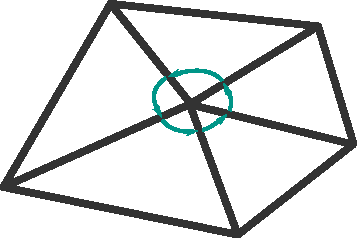
\includegraphics[height=4cm]{figures/NormalCycle1}
    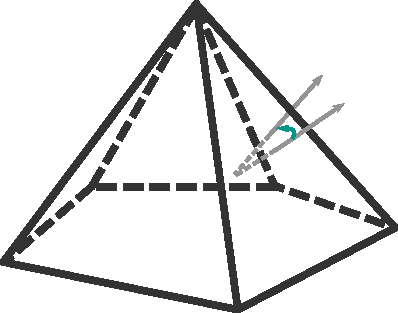
\includegraphics[height=4cm]{figures/NormalCycle2}
    \end{center}}
    \caption{Principe de l'estimation de courbure des cycles normaux. La courbure gaussienne est calculée avec la somme des angles des arêtes incidentes au point concerné (\emph{à gauche}) et la courbure gaussienne avec la somme des angles des normales des faces incidentes au point (\emph{à droite}).
      \label{fig:normal-cycle}}
\end{figure}

Enfin, ils proposent des propriétés de convergence de ces mesures de courbure
sous certaines conditions. Soit $\mathcal{P}$ un sous-ensemble fini de $\dS$,
$T$ la triangulation de Delaunay de $\mathcal{P}$ restreinte à $\Shape$, et
$\epsilon$ la densité de l'échantillonnage de la surface. Si $\mathcal{P}$ est
le $\epsilon$-échantillonnage de $\dS$, \cad si la boule $\Ball{\epsilon
lfs(\vx)}{\vx}$ centrée au point $\vx$ et de rayon $lfs(\vx)$ rencontre
$\mathcal{P}$. Le $lfs(\vx)$ (pour \anglais{local feature size}) correspond à la
distance entre $\vx$ et l'axe médian de $\Shape$. Pour résumer, cela signifie
que l'échantillonnage doit être plus dense sur les zones à forte courbure.
Alors, lorsque $\epsilon < 0.08$ :
%
\begin{align}
  &|\phi^\GaussCurv_T(B) - \tilde{\phi}^\GaussCurv_V(\pi(B)) | \le K\epsilon \,,\\
  &|\phi^\MeanCurv_T(B)  - \tilde{\phi}^\GaussCurv_V(\pi(B)) | \le K\epsilon \,,
\end{align}
%
avec $\pi$ la projection sur $M$ (grâce à $\epsilon < 0.08$, $\pi$ est défini
sur $\Boundary T$ et est un homéomorphe de $\Boundary T$ vers $M$ ), et $K$ une constante.


Les deux principaux problèmes avec cette méthode sont son inadaptabilité face à
des données digitales en ce qui concerne l'échantillonnage et les contraintes
sur la topologie, et le fait que la mesure se fait sur un ensemble de
points et non pas ponctuellement.
%
\paragraph{Invariants par intégration}
%
Enfin, en \emph{traitement géométrique}, d'intéressants outils mathématiques ont
été développés pour concevoir des estimateurs différentiels sur des surfaces
lisses basées sur les invariants par intégration
(\cauthors{Pottmann}{Pottmann2007,Pottmann2009}). Cela consiste à déplacer une
boule le long de la surface de la forme et à calculer des intégrales sur
l'intersection entre la forme et la boule. Les auteurs ont démontré que ces
quantités par intégration apportent d'intéressantes informations de courbures
lorsque le rayon de la boule tend vers zéro. Ils amènent également des preuves
de stabilité --- dans le cas d'échantillonnage de maillage par exemple ---
dépendant de la taille de la boule et du paramètre d'échantillonnage $\epsilon$.
Nos travaux sur les estimateurs digitaux de courbures se basant sur la même
idée, nous détaillerons cette approche dans un prochain paragraphe
(\RefSection{sec:pottmann-principle}).
%
\subsection{Estimation de courbure sur des nuages de points}
%
\paragraph{Ajustement polynomial des jets osculateurs}
%
Lorsque nous avons des nuages de points, la façon la plus naturelle d'approcher
la courbure est de faire correspondre une surface polynomiale de degré $2$ ou
plus à l'ensemble de points. Le meilleur représentant de ces techniques est
l'estimation des quantités différentielles par ajustement polynomial des jets
osculateurs (\anglais{osculating jets}) de \cauthors{Cazals}{Cazals2005}. Un jet
est un développement de Taylor tronqué, un $n$-jet est un développement de
Taylor tronqué à l'ordre $n$. L'intérêt de ces jets est qu'ils contiennent des
informations sur les quantités géométriques locales (tangentes / normales,
courbures principales, etc.).
%
%
Ainsi, le développement de Taylor d'une courbe à l'ordre $n$ équivaut à :
%
\begin{align}
  &f(x) \EqDef J_{B,n}(x) + O(x^{n+1}) \,, \\
  &J_{B,n}(x) \EqDef B_0 + B_1x + B_2x^2 + B_3x^3 + \cdots + B_nx^n \,.
\end{align}
%
Dans le cas d'une surface, nous avons :
%
\begin{align}
  &f(x,y) \EqDef J_{B,n}(x,y) + O(||(x,y)||^{n+1}) \,, \\
  &J_{B,n}(x,y) \EqDef \sum_{k=1}^{n} \left( \sum_{j=0}^{k} B_{k-j,j}x^{k-j}y^j \right) \,,
\end{align}
%
où les développements tronqués de Taylor $J_{B,n}(x)$ et $J_{B,n}(x,y)$ sont les
$n$-jets. Il est à noter que le terme de jet osculateur désigne les $2$-jets.
Ainsi, comme les $n$-jets contiennent des propriétés différentielles de la
courbe/surface de l'ordre $n$, cela implique que toutes les quantités
différentielles de l'ordre $n$ peuvent être calculées grâce aux $n$-jets. Ce qui
nous intéresse ici, ce sont les informations reliées à la courbure contenues
dans les jets osculateurs.


Le principe est simple : (1) collecter les $N$ voisins du point $\vp$, (2)
résoudre l'ajustement polynomial, (3) récupérer les quantités différentielles.
%
%
Pour la première étape, dans le cas d'un maillage, cela correspond à récupérer
les $N$ points voisins à $\vp$ en partant du $1$-voisinage puis en augmentant
progressivement jusqu'à atteindre $N$ points.
% Dans le cas d'un nuage de points,
% il faut d'abord estimer la normale au point $\vp$ et les $N$ points voisins
% peuvent alors facilement être récupérés avec un diagramme de puissance sur le
% plan tangent estimé (nécessite cependant que l'échantillonnage soit assez
% dense).
%


%
Ensuite, il faut effectuer une analyse en composantes principales (\ACP) de
notre ensemble de points voisins afin d'estimer la normale au point $\vp$. Cela
nous permet de placer le point $\vp$ à l'origine du repère et de changer de
système de coordonnées pour celui de Monge (l'axe $\vec{z}$ est aligné avec la
normale, et les axes $\vec{x} et \vec{z}$ sont alignés avec les directions
principales de courbure $\PrincDir{1}$ et $\PrincDir{2}$). Alors :
%
\begin{align} \label{eq:monge}
  f(x,y) = & \frac{1}{2}(\PrincCurv{1}x^2 + \PrincCurv{2}y^2)+ \frac{1}{6}(b_0x^3+3b_1x^2y+3b_2xy^2+b_3y^3) \\ & +\frac{1}{24}(c_0x^4+4c_1x^3y+6c_2x^2y^2+4c_3xy^3+c_4y^4) + O(||(x,y)||^{5}) \,.
\end{align}
%
où $\PrincCurv{1}$ et $\PrincCurv{2}$ sont les courbures principales, $b_0$ et
$b_3$ sont les dérivées directionnelles de $\PrincCurv{1}$ et $\PrincCurv{2}$ le
long de leur ligne de courbure respective, et $b_1$ et $b_2$ sont les dérivées
directionnelles de $\PrincCurv{1}$ et $\PrincCurv{2}$ le long de l'autre ligne de
courbure.
%


%
Enfin, en ayant recours à de l'ajustement de polynômes, nous pouvons récupérer
les $n$-jets de la surface dans ce système de coordonnées. Nous calculons alors
la base de Monge $(\PrincDir{1}, \PrincDir{2}, \NormalDir)$ afin d'en extraire
les coefficients $\PrincCurv{1}$, $\PrincCurv{2}$, $b_0$, $b_1$, $b_2$, $b_3$,
$c_0$, $c_1$, $c_2$, $c_3$ et $c_4$ de l'\RefEquation{eq:monge}.


% Une propriété utile de la forme de Monge
%
%  Ainsi, l'ajustement polynomial peut être calculé en
% supprimant la coordonnée dont l'angle est le plus proche de la normale. Calcul de
% la matrice de Vandermonde $N \times N_n$ :
% %
% \begin{equation}
%   M =  (1,x_i, y_i, x^2_i, \cdots, x_iy_i^{n-1}, y_i^n)_{i=1,\cdots,N} \,,
% \end{equation}
% %
% À noter que cette matrice doit être mise à l'échelle avec la valeur moyenne des
% normes $||(x_i,y_i)||$. Ainsi, résoudre avec la décomposition en valeurs singulières
% (\anglais{Singular Value Decomposition}).
% %
% \todoInlineJeremy{pour récup la normale ?}
% %
% %\\
% %
% Enfin, calculer l'opérateur de forme (appelé également application de
% Weingarten) nous permet de retrouver des informations du second ordre puisqu'il
% est relié aux coefficients des formes fondamentales par les équations de
% Weingarten.
%
% \\
%
Les auteurs proposent des résultats de convergence en $O(\delta^2)$ lorsque la
donnée d'entrée est un échantillonnage de la surface, $\delta$ étant la densité
de points. Cependant, lorsque les données présentent du bruit, aucun résultat
théorique n'est apporté malgré le fait qu'en pratique l'approximation aux
moindres carrés des jets osculateurs est très robuste.
%
Nous nommerons cet estimateur par la suite \JetFitting lors de notre analyse comparative.
%
\paragraph{Mesure de covariance des cellules de Voronoï}
%
Une autre famille de techniques utilise le diagramme de Voronoï
\cite{Alliez2007,Merigot2009,Merigot2011,Cuel2014DGCI} principalement pour
estimer les normales, mais peuvent également extraire des informations de
courbure. L'idée principale derrière cette approche est qu'au lieu de faire des
correspondances dans l'espace tangent à la surface, d'estimer au mieux dans
l'espace orthogonal. \cauthors{Mérigot}{Merigot2011} proposent alors d'associer
en chaque point $\vp$ une \emph{mesure de covariance des cellules de Voronoï}
$\mathcal{V}_{K,R}$ (\VCMM --- \VCM ---) pour une forme $K$. Cette mesure
contient des informations sur la géométrie sous-jacente (voir la
\RefFigure{fig:merigot-VCM-c}).
%

\begin{figure}[ht]{
    \begin{center}
    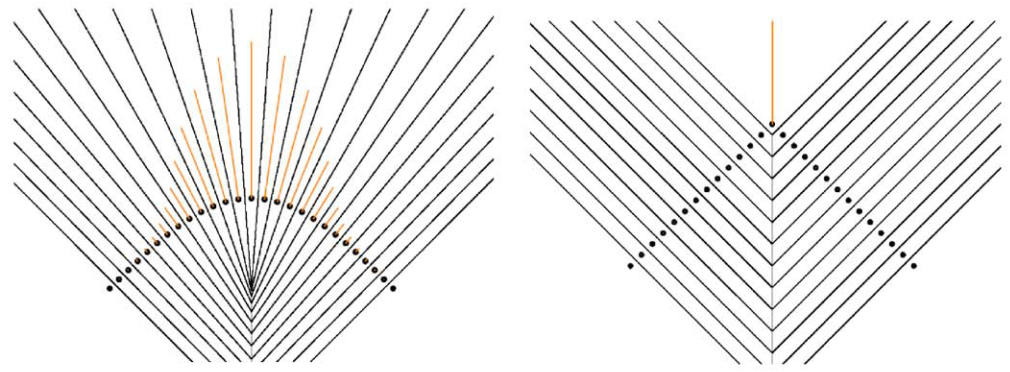
\includegraphics[height=4cm]{images/Feature/VCM}
    \end{center}}
    \caption[Principe de \VCM.]{Principe de \VCM (Figure~2 de \cite{Merigot2011}). En noir : séparation des cellules de Voronoï, en orange : longueur des directions des cellules de Voronoï.
      \label{fig:merigot-VCM-c}}
\end{figure}

Cela nécessite de calculer un matrice de covariance ($cov$) sur les cellules de
Voronoï ($Vor_K$) des points $\vp$ du bord de l'objet :
%
\begin{equation}
    cov(K,\vp) \EqDef \int_K (\vx - \vp)(\vx - \vp)^T d\vx .
\end{equation}
%
Afin d'avoir une information locale de la variation de la forme, les auteurs se
limitent à un voisinage de rayon $R$ (voir la \RefFigure{fig:VCM-multiscale-c}) :
%
\begin{equation}
  \mathcal{V}_{K,R}(\{\vp\}) \EqDef cov(Vor_K(\vp) \cap \Ball{R}{\vp}, \vp) .
\end{equation}

\begin{figure}[ht]{
    \begin{center}
    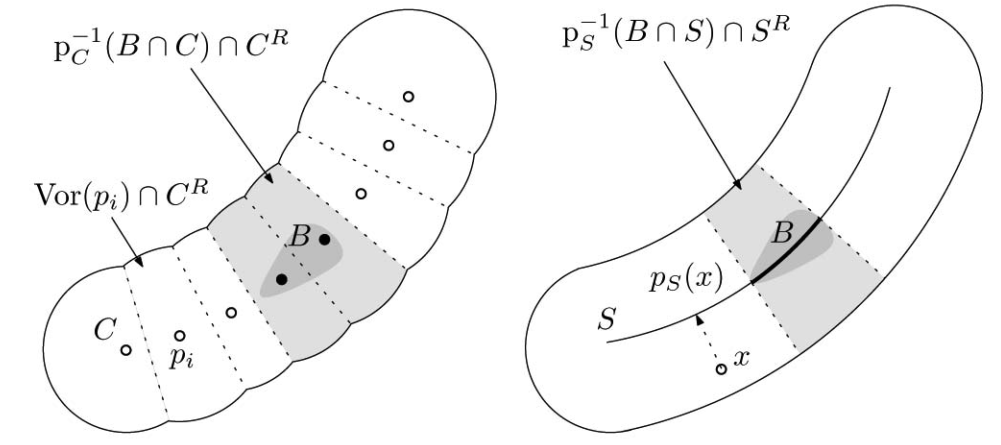
\includegraphics[height=6cm]{images/Feature/VCM_notations}
    \end{center}}
    \caption[Notations de \VCM.]{Notations de \VCM (Figure~5 de \cite{Merigot2011}). La figure de gauche est sur un nuage de points tandis que celle de droite est sur une forme continue. \label{fig:VCM-multiscale-c}}
\end{figure}

Et, afin d'être plus résistant au bruit de Hausdorff, ils utilisent une
version convoluée de \VCM grâce à une fonction indicatrice $\chi_r$
(ayant pour paramètre un rayon $r$) :
%
\begin{equation}
  \mathcal{V}_{K,R} \ast \chi_r(\{\vp\}) \EqDef \int_{K^R} (\vx - \pi^K(\vx))(\vx - \pi^K(\vx))^T \chi(\pi^K(\vx) - \vp) d\vx .
\end{equation}
%
où $\pi^K(\vx)$ est la projection de tout point $\vx$ vers le point le plus
proche de $K$. $\chi_r$ peut être une fonction « Ball » ($\chi_r(\vp) = 1$ si
$\vx$ appartient à $\Ball{r}{\mathbf{0}}$, $0$ sinon) ou encore une fonction «
Hat » ($\chi_r(\vp) = max(0, r - ||\vp||^2)$).
%
Alors, si $\vp$ est un point lisse de $K$, les valeurs propres de
$\mathcal{V}_{K,R} \ast \chi_r$ sont proportionnelles à (respectivement) : $1$,
$\PrincCurv{1}^2(\vp)\frac{r^2}{4}$ et $\PrincCurv{2}^2(\vp)\frac{r^2}{4}$.
%


%
La mesure de covariance convoluée est particulièrement intéressante car cette
mesure apporte de la robustesse même pour des ensembles compacts arbitraires, en
$O(\sqrt{\epsilon})$. C'est en quelque sorte la mesure intégrale de la matrice
de covariance du cône de normale autour du point d'intérêt. Néanmoins, la
convergence des courbures est dépendante de plusieurs paramètres $r$ et $R$ qui
contribuent de manière contradictoire avec l'erreur de Hausdorff. En pratique,
cette approche donne des résultats comparables à \JetFitting pour les courbures.

À noter que \cauthors{Cuel}{Cuel2014DGCI} ont défini une variante digitale du
\VCM ($\DigShape \in \Z^3$) :
%
\begin{equation}
  \hat{\mathcal{V}}_{\DigShape,h,R} \ast \chi_r(\{\vp\})) \EqDef \sum_{\vx \in \Omega_h^R} h^3 (\vx - \pi^{\DigShape}(\vx)) (\vx - \pi^{\DigShape}(\vx))^t \chi(\pi^{\DigShape}(\vx)) ,
\end{equation}
%
où $\Omega_h^R$ est l'ensemble des (centres de) voxels entièrement contenus dans
$\DigShape^R$ (la $R$-dilatation de $\DigShape$) au pas de discrétisation $h$.
La convergence asymptotique de cette variante digitale de l'estimateur \VCM pour
les normales a été prouvée (bord de la surface de classe $C^2$ et de reach $\rho >
0$) \cite{Cuel2014DGCI}.
%
\paragraph{Accumulateur sphérique}
%
Récemment, plusieurs auteurs ont développés de nouvelles approches intéressantes
pour estimer les champs de normales sur des nuages de points bruités, même en
présence de singularités \cite{Li2010, Boulch2012, Zhang2013}. Cela nécessite de
mettre en place un accumulateur auquel les données vont contribuer. La
transformée de Hough \cite{Hough1962} est traditionnellement employée, pour
détecter des formes paramétriques simples comme des lignes ou des arcs de cercle
\cite{Duda1972}. Cependant, elle peut être étendu en dimension 3 :
l'accumulateur n'est plus une image, mais un objet 3D.
\cauthors{Boulch}{Boulch2012} utilisent une boule accumulatrice (voir la
\RefFigure{fig:hough-ball}) de $M$ réceptacles (\anglais{bins}).

\begin{figure}[ht]{
    \begin{center}
    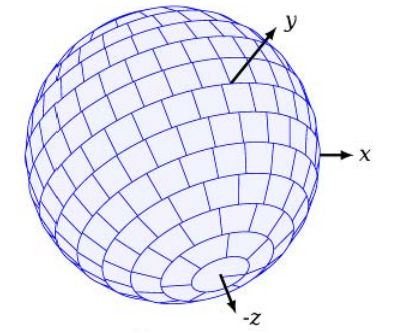
\includegraphics[height=6cm]{images/Curvature/Hough_ball}
    \end{center}}
    \caption[Boule accumulatrice.]{Boule accumulatrice (Figure~3 de \cite{Borrmann2011}). \label{fig:hough-ball}}
\end{figure}

Alors, les auteurs découpent le nuage de points en ensemble de plans (définis
par trois points) et normales. Si le plan est loin d'un coin ou d'une
singularité, alors la normale est correct. Cependant, si ce plan est près d'un
coin, la normale est perturbée par cette singularité (voir la
\RefFigure{fig:Hough-bad} à gauche).

\begin{figure}[ht]{
    \begin{center}
    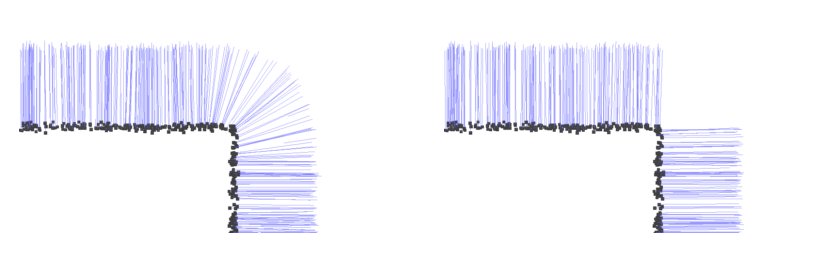
\includegraphics[width=15cm]{images/Curvature/Hough_bad}
    \end{center}}
    \caption[Erreur de reconstruction de normales et correction.]{Erreur de reconstruction de normales et correction (Figure~1 de \cite{Boulch2012}). \label{fig:Hough-bad}}
\end{figure}

Les normales sont accumulés dans la boule accumulatrice, permettant à chaque
plan de contribuer à un vote. Ils utilisent également la transformée aléatoire
de Hough. La différence avec la transformée de Hough traditionnelle est qu'un
point ne vote pas pour toutes les primitives auxquels il appartient. Le vote est
associé à une primitive calculée à partir d'un sous-ensemble de points
\cite{Xu1990, Xu1993} dont le nombre est défini par l'utilisateur comme
condition globale. Enfin, les normales sont redistribuées aux plans en fonction
des bins les plus votés, en moyennant les normales dans ces bins (voir la
\RefFigure{fig:Hough-bad} à droite).


Les principaux inconvénients de cette méthode est que nous obtenons un effet de
regroupement par bin des résultats, de segmentation des données. Cet effet est
surtout visible avec des données bruitées. Ensuite, les bins utilisés sont
anisotropes. Les auteurs rectifient cela en proposant de calculer l’algorithme
plusieurs fois en tournant aléatoirement la boule accumulatrice pour limiter cet
effet. Expérimentalement, ils avancent que cet effet est estompé au bout de $5$
rotations.


\nauthors{Boulch} apportent des résultats de convergence probabilistes.
Cependant, ces méthodes ne peuvent pas être utilisées directement pour le calcul
de courbure : ils peuvent être utilisées en parallèle avec des techniques
d'estimation de courbure pour détecter les singularités sur la surface dans un
premier temps, et de limiter l'estimation de la courbure aux zones lisses.
%
\paragraph{Théorie des varifolds}
%
Enfin, une approche très récente venant de la théorie de la mesure géométrique
utilise la théorie de \anglais{Varifolds} \cite{Almgren1965} pour concevoir une
robuste estimation de la courbure moyenne \cite{Buet2014,Buet2015}. Cette
théorie est suffisamment générique pour fonctionner sur des variétés lisses, des
maillages discrets, des nuages de points ainsi que sur des données digitales.
Afin de mener à bien l'estimation géométrique, cette approche nécessite d'avoir
une position et une approximation des normales. Si les deux prérequis
convergent, alors la première variation régularisé de la mesure de Varifold
converge vers la courbure moyenne. La vitesse de convergence de cette approche
ainsi que sa précision en pratique restent à explorer.
%
\subsection{Estimation de courbure sur des surfaces digitales}
%
%BC [Esbelin2011], MDSS [Coeurjolly2001;deVieilleville2007] et MDCA [Roussillon2011].
Comme vu dans le \RefChapitre{sec:notions}, en géométrie digitale nous
considérons la convergence asymptotique comme un critère essentiel pour un
estimateur \cite{Klette2000}. Lorsque la forme est discrétisée
sur une grille avec une résolution $h$ tendant vers zéro, la quantité estimée
devrait converger vers la valeur attendue.


\cauthors{Coeurjolly}{Coeurjolly_ChapEstimateur} ont proposé un état de l'art
complet pour l'estimation de tangentes et de la courbure en dimension 2. Nous
allons détailler les méthodes les plus représentatives.
%
\paragraph{Reconnaissance d'objets digitaux}
%
Nous allons nous intéresser dans un premier temps aux méthodes reconnaissant des
objets digitaux sur le bord de l'objet, afin d'en extraire des informations
différentielles.


\noindent\textbf{Segments digitaux maximaux.\quad}
% The curvature k is defined from the length l and the width w of a DSS as follow: $1/k=(l \ast l)/(8 \ast w)+w/2$
% Most centered Maximal Segment
\cauthors{Coeurjolly}{Coeurjolly2001} ont montré une façon simple d'estimer
la courbure à la surface d'un objet digital à l'aide des segments maximaux.
Cette méthode, que nous appellerons \MDSS par le suite, propose de calculer la
longueur des segments maximaux du bord $\Boundary \DigShape$ de $\DigShape
\subset \Z^2$. En effet, il existe une relation entre la corde d'un cercle et
son rayon (voir \RefFigure{fig:mdss-chord}).

\begin{figure}[ht]{
    \begin{center}
    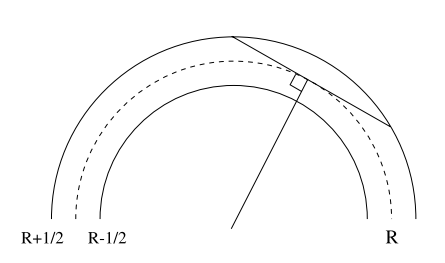
\includegraphics[width=10cm]{images/Notions/MDSS1}
    \end{center}}
    \caption[Relation entre la corde d'un cercle et son rayon.]{Relation entre la corde d'un cercle et son rayon (Figure~3 de \cite{Coeurjolly2001}). \label{fig:mdss-chord}}
\end{figure}

L'idée ici est de considérer le segment maximal comme une corde à une distance
$h$ (la taille de la grille) du cercle osculateur de la surface.
Alors, si $l$ est la longueur du MDSS au point $\vp \in \Z^2$, nous avons :
%
\begin{equation}
  %
    \frac{1}{\Curv(\vp,\DigShape)} = \frac{(l \cdot l)}{8} + \frac{1}{2} \,.
  %
\end{equation}
%
Une version plus robuste est proposée en ajoutant l'épaisseur du MDSS $w$ :
%
\begin{equation}
  %
    \frac{1}{\Curv(\vp,\DigShape)} = \frac{(l \cdot l)}{8 \cdot w} + \frac{w}{2} \,.
  %
\end{equation}
%
Cependant, aucune preuve de convergence n'est apporté pour cet estimateur.
% => ça c'est pour les demi tangentes, erreur dans le bouquin ?
% La méthode repose sur l'hypothèse que les segments maximaux
% d'un cercle euclidien se comportent comme des cordes de hauteur $h$ (le pas de
% discrétisation) et de longueur $\Theta(h^{-\frac{1}{2}})$. Cependant, quelques
% années plus tard, \cauthors{de Vieilleville}{deVieilleville2007} remarquent que
% bien que la borne supérieure du plus long MDSS est en $O(h^{-\frac{1}{2}})$, leur
% longueur en moyenne est proche de $\Theta(h^{-\frac{1}{3}})$ (entre
% $\Theta(h^{-\frac{1}{3}})$ et $\Theta(h^{-\frac{1}{3}} \log
% \left(\frac{1}{h}\right))$, voir le \RefLemma{lem:law-length-MDSS}). Cette borne
% supérieure a pour conséquence de réfuter la preuve de convergence avancée dans
% \cite{Coeurjolly2001}.
%
%
% \textbf{Demi-tangentes digitales}\\
% %
% \cauthors{de Vieilleville}{deVieilleville2007} s'intéressent à la reconnaissance
% des segments maximaux digitaux que nous avons défini dans le chapitre précédent
% (voir \RefSection{sec:segments}). Ainsi, le principe est simple : pour une forme
% $\Shape \subset \R^2$, pour chaque point $\vp$ du bord digital $\BdZ{\DigShape}$
% avec $\DigShape = \DSh$, ils récupèrent le segment digital maximal (\MDSS) dont
% son centre est le plus proche du point $\vp$. Alors, en s'appuyant sur des
% travaux de \cauthors{Coeurjolly}{Coeurjolly2001}, en calculant l'inverse du
% rayon du cercle circonscrit contenant $\vp$ et les deux extrémités du \MDSS le
% plus proche que nous aurons mis à l'échelle avec le pas de discrétisation $h$,
% nous obtenons une estimation de la courbure.
% %
% \\
% %
% Cependant, les auteurs annoncent ne pas pouvoir prouver la convergence
% asymptotique de cet estimateur de courbure à cause d'une propriété sur les
% demi-tangentes sur le bord digital qui ne peut pas être vérifiée, la convergence
% de l'estimateur reposant sur celle-ci.
% %


\noindent\textbf{Analyse des arcs de cercle digitaux maximaux.\quad}
% Most centered Digital Circular Arc
\cauthors{Roussillon}{Roussillon2011} proposent non plus d'étudier les segments
maximaux digitaux, mais de reconnaître des arcs de cercle maximaux digitaux
(\MDCA, voir \RefDefinition{def:digital-circular-arc} pour la définition
formelle). La courbure d'une courbe étant définie comme l'inverse du rayon du
cercle osculateur, il parait logique de s'intéresser à reconnaître des arcs de
cercle digitaux sur la forme digitale.

\begin{figure}[ht]{
    \begin{center}
    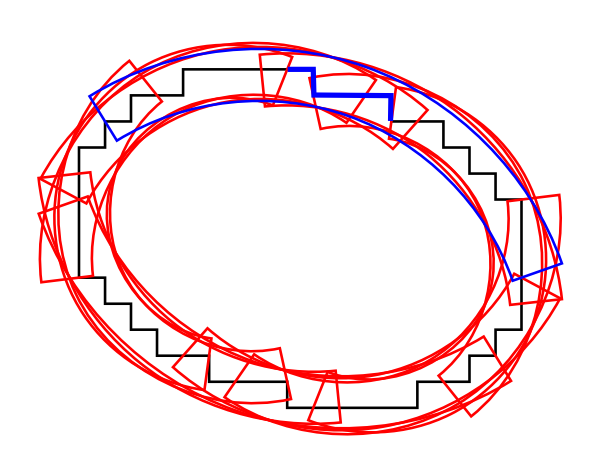
\includegraphics[height=6cm]{images/Notions/MDCA}
    \end{center}}
    \caption[Illustration des arcs de cercle digitaux maximaux sur une ellipse.]
    {Illustration des arcs de cercle digitaux maximaux sur une ellipse (Figure~1
    de \cite{Roussillon2011}).\label{fig:mdca-curv-figure}}
\end{figure}

Le principe de l'estimateur est simple : pour une forme $\Shape \subset \R^2$
avec un champ de courbure continu, ils calculent les $(A_i)_{i \in 1,n}$ \MDCA
($n$ étant le nombre totale de \MDCA) du bord digital $\BdZ{\DigShape}$ avec
$\DigShape = \DSh$. Ils calculent également les $(V_i)_{i \in 1,n}$, une
partition du bord digital permettant de faire correspondre tous les surfels vers
le \MDCA le plus proche. Chaque surfel est relié à son \MDCA le plus
représentatif (voir \RefFigure{fig:mdca-curv-figure}, les surfels bleus sont
reliés au \MDCA bleu). Alors :
%
\begin{equation}
  %
    \forall i \in 1,\cdots,n, \quad \forall \ve \in V_i, \quad \forall \vp \in \ve,
    \quad \CurvH{}_{MDCA}(\DigShape,\vp,h) \EqDef \Curv(A_i,h) \,.
  %
\end{equation}
%
Les auteurs ont prouvé la convergence asymptotique en $O(h^{\min(1-2a,b)})$ de
cet estimateur sur des formes convexes de $\R^2$ dont le champ de courbure est
continue, strictement positif et borné supérieurement, si $0 < b \le a <
\frac{1}{2}$ correspond aux bornes inférieures et supérieurs des longueurs des
\MDCA (\respp $\Omega(h^a)$ et $O(h^b)$). Cette dernière hypothèse n'est pas
prouvé à ce jour.


Le principal avantage de ces deux méthodes est qu'elles ne nécessitent aucun
paramètre. Cependant, ces méthodes de reconnaissances d'objets sont assez
sensibles lorsque les données sont bruités. C'est ce que nous verrons dans la
section comparative (\RefSection{sec:comparaison-courbure}).
%
\paragraph{Convolutions binomiales}
%
\cauthors{Malgouyres}{Malgouyres2008} ont proposé une méthode pour estimer les
dérivées sur le principe de convolutions binomiales (nous la nommerons \BC par
la suite). Ils définissent un opérateur $\Psi_K$ qui modifie la fonction $F : \Z
\rightarrow \Z$ par la convolution avec un noyau $K : \Z \rightarrow \Z$. Par
exemple, l'opérateur de différence finie arrière est $\Psi_\delta F$ où le noyau
$\delta$ est défini comme :
%
\begin{equation}
  %
    \delta(a) =
      \begin{cases}
        1   & \text{si } a = 0,\\
        -1  & \text{si } a = 1,\\
        0   & \text{sinon}.\\
      \end{cases}
  %
\end{equation}
%
Les auteurs donnent également un noyau de lissage défini par (pour $n \in \N$) :
%
\begin{equation}
  %
  H_n(a) =
    \begin{cases}
      \left(\!
        \begin{array}{c}
          n \\
          a + \frac{n}{2}
        \end{array}
        \!\right)   & \text{si } n \text{ est pair et } a \in \{ -\frac{n}{2}, \cdots, \frac{n}{2},\\
        \left(\!
          \begin{array}{c}
            n \\
            a + \frac{n + 1}{2}
          \end{array}
          \!\right)   & \text{si } n \text{ est impair et } a \in \{ -\frac{n + 1}{2}, \cdots, \frac{n - 1}{2},\\
      \quad\quad 0   & \text{sinon}.\\
    \end{cases}
  %
\end{equation}
%
Alors, le noyau de dérivées $D_n$ est défini par :
%
\begin{equation}
  D_n \EqDef \delta \ast H_n \,,
\end{equation}
%
où $\ast$ est le produit de convolution. L'estimateur de dérivés pour une fonction discrète $F$ est :
%
\begin{equation}
  \frac{1}{2^n}\Psi_{D_n}F \,.
\end{equation}
%
Les auteurs proposent également des dérivées d'ordre supérieur avec une
expression similaire :
%
\begin{align}
  D_n^2 &= \delta \ast \delta \ast D_n \\
  D_n^k &= \underbrace{\delta \ast \cdots \ast \delta}_{k \text{ fois}} \ast D_n \,.
\end{align}
%
La courbure est alors estimée de la sorte :
%
\begin{equation}
  %
  \CurvH{n}_{BC}(\vp) \EqDef \frac{D_n^2(\vp_1) \ast D_n(\vp_2) - D_n^2(\vp_2) \ast D_n(\vp_1)}{(D_n(\vp_1)^2 + D_n(\vp_2)^2)^\frac{3}{2}} \,.
  %
\end{equation}


Dans le cas où $n = \lfloor h^{2(\alpha -3)/3} \rfloor$ et $\alpha \in ]0,1]$ est un paramètre
associé au niveau de bruit (plus $\alpha$ est proche de $0$, plus l'estimateur
sera robuste au bruit), \cauthors{Esbelin}{Esbelin2011} annoncent une convergence asymptotique en
$O(h^{{(\frac{2}{3})}^k})$ des dérivées du $k$-ième ordre pour des formes $C^3$ (donc en
$O(h^{4/9})$ pour les dérivées du second ordre). Nous verrons dans la partie
comparative que nous n'observons expérimentalement pas la même vitesse de
convergence (\RefSection{sec:comparaison-courbure}).
%
\paragraph{Correspondance de surface polynomiale}
%
\cauthors{Provot}{Provot2011} proposent quant à eux de s'intéresser aux
\anglais{Digital Level Layer} (\DLL) pour estimer les dérivées d'une fonction
digitale à l'aide de la programmation linéaire ou avec des outils de la
\AlgorithmicGeometry. Cette approche permet d'approcher les $k$ dérivées de
$f^{(k)}(\vx)$. Ainsi, à l'instar de \JetFitting, ils proposent une nouvelle
méthode basées sur les polynômes de Taylor.
%
Le principe de cette méthode est de faire ajuster un polynôme sur les valeurs de
la fonction digitale. Ils étendent alors les valeurs de la fonction $F(\vx)$
dans l'intervalle $[F(\vx) - R; F(\vx) - R]$. Il suffit alors juste de trouver
un polynôme $P(\vx)$ respectant :
%
\begin{equation}
    F(\vx) - R \le P(\vx) \le F(\vx) + R \,,
\end{equation}
%
dans le voisinage de $\vx_0$, où $P(\vx) = \sum_{i=1}^{k} a_i\Shape^i$, $a_i$
étant les coefficients entiers du polynôme $P(\vx)$. Ils introduisent alors la notion de
rugosité (\anglais{roughness}) de la fonction, \cad le $R$ minimum nécessaire
pour trouver un polynôme s'ajustant sur les données de la fonction $F$ avec une
erreur inférieure à $R$ (voir la \RefFigure{fig:dll-roughness}).

\begin{figure}[ht]{
    \begin{center}
    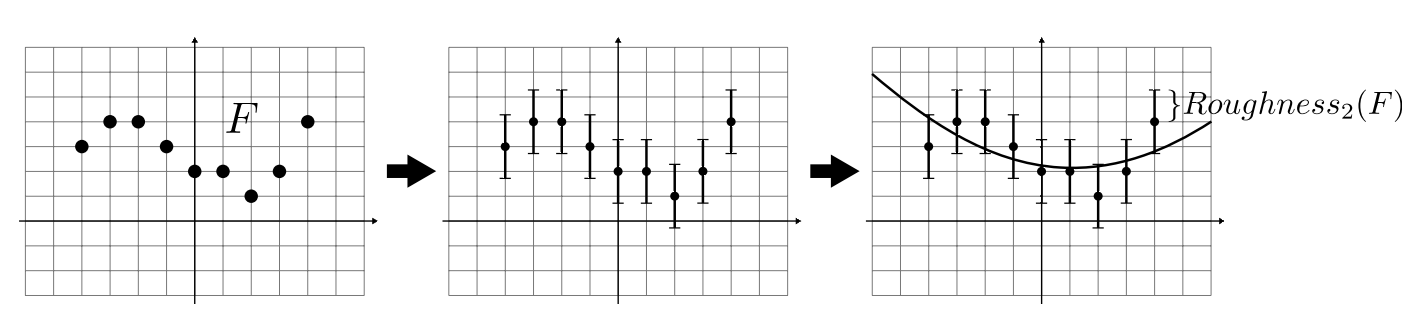
\includegraphics[width=14cm]{images/Curvature/DLL_roughness}
    \end{center}}
    %
    \caption[Illustration du paramètre $R$ de rugosité de \DLL.]{\emph{De gauche à
    droite : } Fonction $F$, $F$ étendu avec un intervalle le plus petit
    possible pour lequel il existe un polynôme de degré 2 ou plus qui passe au
    travers de chaque point étendu (Figure~1 de
    \cite{Provot2011}).\label{fig:dll-roughness}}
    %
\end{figure}

Alors, ils montrent que nous pouvons calculer la rugosité comme l'épaisseur
verticale (\anglais{vertical thickness}) d'un ensemble $S = \{((\vx^i)_{1 \le i
\le k} \; F(\vx)) \text{ pour } \vx \in \Shape \}$ de dimension $k + 1$ (voir la
\RefFigure{fig:dll-roughness2}). Ils utilisent alors l'algorithme de détection
de collision Gilbert-Johnson-Keerthi (GJK) \cite{Gilbert1988} pour calculer
rapidement l'épaisseur verticale de l'ensemble $S$ (l'épaisseur de la séparation
entre deux hyperplans).

\begin{figure}[ht]{
    \begin{center}
    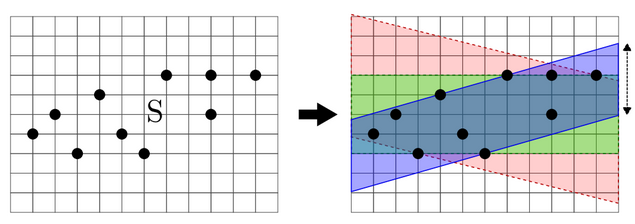
\includegraphics[width=14cm]{images/Curvature/DLL_roughness2}
    \end{center}}
    %
    \caption[Illustration de la notion d'épaisseur du \DLL.]{Illustration de la
    notion d'épaisseur du \DLL. Les trois bandes s'ajustent sur les points de
    $S$ (en prenant en compte une direction $\vec{d}$, vertical dans le cas présent).
    La bande bleue possède alors l'épaisseur minimale de toutes les bandes
    (Figure~10 de \cite{ProvotIPOL2014}).\label{fig:dll-roughness2}}
    %
\end{figure}

Enfin, ils définissent la $k$-ième dérivée de $F$ à l'origine comme :
%
\begin{equation}
    F^{(k)}(\mathbf{0}) \EqDef k!a_k \,,
\end{equation}
%
si $P(\vx)$ respecte les contraintes de rugosité de ses bornes.

Ils obtiennent alors une preuve de convergence en $O(h^{\frac{1}{k+1}})$ sur
l'estimation des dérivées du $k$-ième ordre pour une fonction réelle $f : \R
\rightarrow \R$ de classe $C^{k+1}$ où les dérivées d'ordre $k+1$ sont bornées
dans le voisinage du point $\vx$. L'inconvénient de cette méthode est qu'elle
dépend énormément du paramètre de rugosité maximale. De plus, cette approche
n'est applicable qu'à des fonctions discrètes, et pas directement à des bords
d'objets discrets.
% ils ne fournissent
%pas de moyen d'extraire la courbure de ces dérivées.
%
%
% Un \DLL est un sous-ensemble de points
% $\vp$ de $\Z^d$ vérifiant la double inégalité suivante :
% %
% \begin{equation}
%     -\delta \le F(\vp) \le \delta
% \end{equation}
% %
% où $F : \Shape \rightarrow \R$ avec $\Shape \subset \R$. L'idée derrière cette
% méthode est de rajouter une contrainte d'épaisseur (ce qu'ils appellent le
% paramètre de rugosité, voir \RefFigure{fig:dll-roughness, fig:dll-roughness2}) au lieu de faire de l'ajustement de polynôme avec de l'erreur aux moindres carrés comme \JetFitting.
% %
% \begin{figure}[ht]{
%     \begin{center}
%     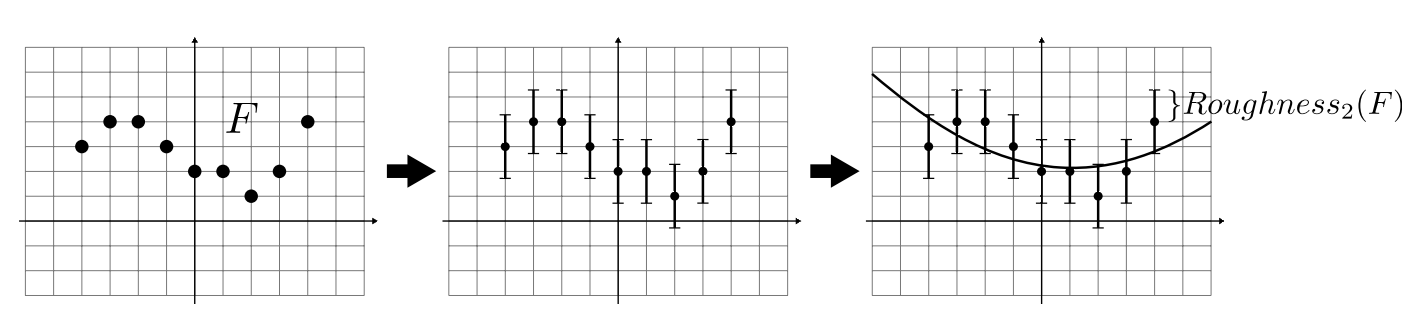
\includegraphics[width=14cm]{images/Curvature/DLL_roughness}
%     \end{center}}
%     %
%     \caption[Illustration des arcs de cercle digitaux maximaux sur une
%     ellipse.]{\emph{De gauche à droite : } Fonction $F$, $F$ étendu avec un
%     intervalle le plus petit possible pour lequel il existe un polynome de degré
%     1 ou plus qui passe  au travers de chaque point étendu (Figure~1 de
%     \cite{Provot2011}).\label{fig:dll-roughness}}
%     %
% \end{figure}
 %
% De plus, cela permet de considérer la forme digitale directement, et ainsi de
% reconnaitre des structures digitales grâce à l'algorithme de détection de
% collision Gilbert-Johnson-Keerthi (GJK) \cite{Gilbert1988}. Ainsi, il permet de décomposer la surface en DSS, DCA et coniques.
% %
% \\
% %
% % La première question que nous pouvons nous poser, c'est pourquoi définir une
% % nouvelle primitive digitale correspondant à des courbures algébriques ou à des
% % surfaces euclidiennes ? Les auteurs justifient ce choix par le fait que les
% % autres primitives digitales ont de chacunes des avantages et des inconvénients,
% % et qu'il est difficile de déterminer laquelle des approches est la plus adaptée.
% % Par exemple les primitives basées sur l'approche analytique peuvent perdre des
% % informations topologiques de la surface. Les primitives basées sur l'approche
% % topologique ou morphologique quant à elles ne possèdent pas de caractérisation
% % analytique. Les \DLL proposent une façon unifiée et efficace pour résoudre
% % toutes ces contraintes.
%
% \begin{figure}[ht]{
%     \begin{center}
%     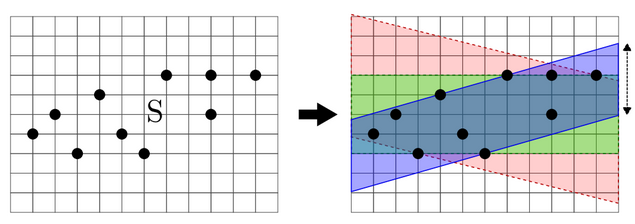
\includegraphics[width=14cm]{images/Curvature/DLL_roughness2}
%     \end{center}}
%     %
%     \caption[Illustration de la notion d'épaisseur du \DLL.]{Illustration de la
%     notion d'épaisseur du \DLL. Les trois bandes s'ajustent sur les points de
%     $S$ (en prenant en compte une direction $\vec{d}$, vertical dans le cas présent).
%     La bande bleue possède alors l'épaisseur minimale de toutes les bandes
%     (Figure~10 de \cite{ProvotIPOL2014}).\label{fig:dll-roughness2}}
%     %
% \end{figure}

% Ils obtiennent alors une preuve de convergence en $O(h^{\frac{1}{k+1}})$ sur
% l'estimation des dérivées du $k$-ième ordre pour une fonction réelle $f : \R
% \rightarrow \R$ de classe $C^{k+1}$ où les dérivées d'ordre $k+1$ sont bornées
% dans le voisinnage du point $\vx$.
%Alors l'estimation de la courbure converge
%asymptotiquement en $O(h^\frac{1}{3})$
% \begin{table}[]
% \centering
% \caption{My caption}
% \label{my-label}
% \begin{tabular}{@{}lp{0.15cm}p{0.15cm}p{0.15cm}p{0.15cm}p{0.15cm}p{4cm}p{2cm}r@{}}
% \hline
% Estimateur & \multicolumn{5}{c}{Courbure} & Famille de formes & Vitesse de convergence & Référence \\ \cline{2-6}
% & $\Curv$ & $\MeanCurv$ & $\GaussCurv$ & $\PrincCurv{i}$ & $\NormalDir$ &  &  & \\ \hline
%
% Gauss-Bonnet & \svgNope & \svgNope & \svgYes & \svgNope & \svgNope & Surface paramétrique lisse de valence $6$ & $O(\delta^\alpha)$ avec $\alpha \ge 3$ & \cite{Xu2006} \\
%
% Cycles normaux & \svgNope & \svgYes & \svgYes & \svgNope & \svgNope & Surface lisse $\epsilon lfs$ & $O(\epsilon)$ & \cite{CohenSteiner2003} \\
%
%
% \MDCA     & \svgYes & \svgNope & \svgNope & \svgNope & \svgNope & ??? & \svgNope & \cite{Coeurjolly2001} \\
% \II       & \svgYes & \svgYes & \svgYes & \svgYes & \svgYes & $\Shapes^{3-SC}$ avec $R = kh^\frac{1}{3}$ & $O(h^\frac{1}{3})$ & \cite{CVIU2014} \\
% \hline
% \end{tabular}
% \end{table}

\begin{table}[ht]
\centering
\caption{Convergence asymptotique connus d'estimateurs de courbure sur des données digitales.}
\label{tab:curv-comp}
\begin{tabular}{@{}p{1.9cm}lllr@{}}
\toprule
 & & \multicolumn{2}{c}{Vitesse de convergence} &            \\ \cmidrule(r){3-4}
Estimateur & Famille de formes & Borne sup. & Observée & Référence \\ \midrule

$\hat{\Curv}^{MDCA}$ & $\Shapes^{1-SC}$ & ? & $O(h^\frac{1}{3})$ & \cite{Roussillon2011} \\
$\hat{\Curv}^{BC}$ & $\Shapes^{3-SC}$ & $O(h^\frac{4}{9})$ & $\approx O(h^{0.154})$ & \cite{Malgouyres2008} \\
$\hat{\Curv}^{MDSS}$ & $\Shapes^{1-SC}$ & ? & \svgNope & \cite{Coeurjolly2001} \\
$\hat{\Curv}^{II}$ & $\Shapes^{3-SC}$ avec $R = kh^\frac{1}{3}$ & $O(h^\frac{1}{3})$ & $O(h^\frac{1}{3})$ & ici \\
$\hat{\Curv}^{*II}$ & $\Shapes^{3-SC}$ & $O\left(h^\frac{1}{3} \log^2 \left(\frac{1}{3}\right)\right)$ & $O(h^\frac{1}{3})$ & ici \\
\midrule
% $\hat{\MeanCurv}^{JetFitting}$ &  & ? & $O(h^\frac{1}{3})$ & \cite{Cazals2005} \\
$\hat{\MeanCurv}^{II}$ & $\Shapes^{3-SC}$ avec $R = kh^\frac{1}{3}$ & $O(h^\frac{1}{3})$ & $O(h^\frac{1}{3})$ & ici \\
$\hat{\MeanCurv}^{*II}$ & $\Shapes^{3-SC}$ & ? & $O(h^\frac{1}{3})$ & ici \\
\midrule
% $\hat{\PrincCurv{i}}^{JetFitting}$ &  & ? & $O(h^\frac{1}{3})$ & \cite{Cazals2005} \\
$\hat{\PrincCurv{i}}^{II}$ & $\Shapes^{3-SC}$ avec $R = kh^\frac{1}{3}$ & $O(h^\frac{1}{3})$ & $O(h^\frac{1}{3})$ & ici \\
$\hat{\PrincCurv{i}}^{*II}$ & $\Shapes^{3-SC}$ & ? & $O(h^\frac{1}{3})$ & ici \\

\bottomrule
\end{tabular}
\end{table}


Ainsi, nous avons quelques estimateurs qui convergent asymptotiquement en
dimension 2 (voir \RefTable{tab:curv-comp}), mais qui peuvent être sensibles au
bruit de la forme ou dont la preuve de convergence repose sur les paramètres
choisis. De plus pour l'estimation de courbure le long de courbes 2D, la
convergence asymptotique d'estimateurs ne nécessitant aucun paramètre représente
toujours un défi (des résultats de convergence d'estimateurs sans paramètre ont
été obtenus pour l'estimation de longueur \cite{Coeurjolly2004} et des normales
\cite{deVieilleville2007}). Nous allons en proposer dans ce chapitre. Enfin, il
n'existe aucun estimateur de courbure en dimension 3 apportant des preuves de
convergence asymptotique \cite{Lenoir1997,Fourey2008}. Nous allons également
palier à ce manque dans ce chapitre.

\section{Estimation de la courbure par intégration volumique locale d'une boule}
\label{sec:estimators:volume}
%
Nous allons désormais nous intéresser aux travaux réalisés au cours de cette
thèse. Nous allons dans un premier temps décrire l'estimation de quantités
différentielles que proposent \cauthors{Pottmann}{Pottmann2007,Pottmann2009},
dans le \RefSection{sec:pottmann-principle}. Nous allons ensuite proposer une
version digitale de ces estimateurs dans les \RefSections{sec:ii-2d}{sec:ii-3d}
en dimension 2 et 3. La principale contribution de ces travaux est de démontrer
la convergence asymptotique de ces estimateurs sur des données digitales. Ces
travaux ont été publiés dans \cite{DGCI2013,CVIU2014}.

\GeometryProcessing, le calcul d'invariants par intégration a été largement
étudié dans le but de définir des estimateurs de quantités différentielles.
\cauthors{Pottmann}{Pottmann2007,Pottmann2009} en ont d'ailleurs fait un
panorama assez complet. L'idée principale de cette approche est de déplacer un support
sur les points $\vx$ du bord $\dS$ d'une forme $\Shape$ et calculer
l'intégrale de l'intersection entre $\Shape$ et ce support. Différents supports
peuvent être considérés (sphère euclidienne, boule euclidienne, etc.) ainsi que
différentes fonctions d'intégration (linéaire, gaussienne, etc.). Nous
n'utiliserons par la suite que les invariants volumiques par intégration définis
de la sorte :
%
\begin{definition}
  \label{def:Volume}
  %
  Pour une forme $\Shape \in \Shapes$ et un rayon $R \in \R^{+*}$, \colorize{l'intégrale
  volumique} $V_R(\vx)$ au point $\vx \in \dS$ est donné par :
  %
  \begin{equation}
    V_R(\vx) \EqDef \int_{\Ball{R}{\vx}} \chi(\vp)d\vp\,,
  \end{equation}
  %
  où $\Ball{R}{\vx}$ est une boule euclidienne de rayon $R$ et de centre $\vx$,
  et $\chi(\cdot)$ est la fonction caractéristique de $\Shape$ (valant $1$ pour
  tous les points de $\Shape$, $0$ sinon). En dimension 2, nous noterons cette
  quantité $A_R(\vx)$.
  %
\end{definition}
%
\subsection{Analyse euclidienne de l'intégration volumique de la boule, et relation à la courbure}
\label{sec:pottmann-principle}
%
La relation entre $A_R(\vx)$ et la courbure (\resp $V_R(\vx)$ et la courbure
moyenne ) au point $\vx$ pour des formes de $\R^2$ (\respp $\R^3$) a beaucoup
été étudiée dans la littérature \cite{Bullard1995,Pottmann2007,Pottmann2009}
Nous pouvons la formaliser ainsi :
%
\begin{lemma}{\textbf{\cite{Pottmann2009}}}\\
\label{lem:pottmann-2d}
  %
  Pour une forme suffisamment lisse $\Shape$ de $\R^2$, $\vx \in \dS$, nous
  avons :
  %
  \begin{equation}
    \label{eq:volume2d}
    A_R(\vx) = \frac{\pi}{2} R^2 - \frac{\Curv(\Shape,\vx)}{3}R^3 + O(R^4)\,.
  \end{equation}
  %
  où $\Curv(\Shape,\vx)$ est la courbure de $\dS$ au point $\vx$.
  %
  \\
  %
  Pour une forme suffisamment lisse $\Shape$ de $\R^3$, $\vx \in \dS$, nous
  avons :
  %
  \begin{equation}
    \label{eq:volume3d}
    V_R(\vx) = \frac{2\pi}{3} R^3 - \frac{\pi \MeanCurv(\Shape,\vx)}{4}R^4 + O(R^5)\,.
  \end{equation}
  %
  où $\MeanCurv(\Shape,\vx)$ est la courbure moyenne de $\dS$ au point $\vx$.
  %
\end{lemma}
%
De tels résultats sont obtenus par approximation de Taylor au point $\vx$ de la
surface $\dS$, approchée sous la forme de la fonction paramétrique $z=f(x,y)$ ($y=f(x)$ en
2D). Alors, des \RefEquations{eq:volume2d}{eq:volume3d} avec un
rayon $R$ fixé, nous pouvons définir les estimateurs locaux de courbure en 2D,
$\CurvT{R}(\vx)$, et de courbure moyenne en 3D, $\MeanCurvT{R}(\vx)$ :
%
\begin{definition}{\fakeTitle{Estimateurs de courbure en 2D $\CurvT{R}(\Shape,\vx)$ et de courbure moyenne en 3D $\MeanCurvT{R}(\Shape,\vx)$ \cite{Pottmann2007}}}
  \label{def:pottmann-2d-3d-mean}
  %
  Pour une forme $\Shape \subset \R^2$, l'estimateur de courbure en 2D $\CurvT{R}$
  au point $\vx \in \dS$ est défini par :
  %
  \begin{equation}
    \label{eq:pottmann-2d}
    \CurvT{R}(\Shape,\vx) \EqDef \frac{3\pi}{2 R} - \frac{3 A_R(\vx)}{R^3} .
  \end{equation}
  %
  \\
  %
  Pour une forme $\Shape \subset \R^3$, l'estimateur de courbure moyenne en 3D
  $\MeanCurvT{R}$ au point $\vx \in \dS$ est défini par :
  %
  \begin{equation}
    \label{eq:pottmann-3d-mean}
    \MeanCurvT{R}(\Shape,\vx) \EqDef \frac{8}{3 R} - \frac{4 V_R(\vx)}{\pi R^4}.
  \end{equation}
  %
\end{definition}
%
De plus, lorsque le rayon $R$ de la boule tend vers zéro, les valeurs de ces
deux estimateurs vont converger vers celles espérées. Plus formellement,
\cauthors{Pottmann}{Pottmann2007} (et les travaux précédents) ont démontré la
convergence des estimateurs de courbure en 2D et de courbure moyenne en 3D :
%
\begin{theorem}{\fakeTitle{Convergence des estimateurs de courbure en 2D $\CurvT{R}(\Shape,\vx)$ et de courbure moyenne en 3D $\MeanCurvT{R}(\Shape,\vx)$ \cite{Pottmann2007}}}
  \label{theo:pottmann-2d-3d-mean-conv}
  %
  \begin{equation}
    \CurvT{R}(\Shape,\vx) = \Curv(\Shape,\vx) + O(R),
    \quad\MeanCurvT{R}(\Shape,\vx) = \MeanCurv(\Shape,\vx) + O(R).
  \end{equation}
  %
\end{theorem}
%
De la même manière, des informations directionnelles comme les courbures
principales (et donc la courbure gaussienne) peuvent être extraites du calcul
par intégration. En effet, à la place de calculer la mesure de $\Ball{R}{\vx}$
dans la \RefDefinition{def:pottmann-2d-3d-mean}, nous allons calculer sa matrice
de covariance :
%
\begin{definition}
  \label{def:cov-matrix}
  Pour un ensemble non vide $Y \subset \R^d$, la matrice de covariance de $Y$
  est définie par :
  \begin{equation}
    \Cov(Y) \EqDef \int_Y (\vp-\overline{Y})(\vp-\overline{Y})^T d\vp = \int_Y \vp \vp^T d\vp - \Vol(Y)\overline{Y}\overline{Y}^T,
  \end{equation}
  où $\overline{Y}$ est le barycentre de $Y$ et $\Vol(Y)$ son volume.
\end{definition}
%
Pour les entiers $p, q, s \ge 0$, nous pouvons écrire la définition des $
pqs$-moments $\Mom{pqs}(Y)$ de $Y$ ($x_i$ est la $i$-ème composante de $\vx$) :
%
\begin{equation}
  \label{eq:moments}
  \Mom{pqs}(Y) \EqDef \iiint_Y x_1^p x_2^q x_3^s dx_1 dx_2 dx_3\,.
\end{equation}
%
Il apparaît alors clairement que le volume $\Vol(Y)$ est le $0$-moment
$\Mom{000}(Y)$, et que le barycentre $\overline{Y}$ est donné par les $1$-moments
normalisés par le $0$-moment, c'est à dire :
%
\begin{equation}
  \overline{Y} \EqDef \frac{( \Mom{100}(Y), \Mom{010}(Y), \Mom{001}(Y) )^T}{\Mom{000}(Y)}
\end{equation}
%
\begin{lemma}\label{lem:moment-ball}
  %
  Soit $\Ball{R}{\vy}$ une boule de rayon $R$ et de centre $\vy$. Alors, pour un
  ensemble non vide $Y \subset \Ball{R}{\vy}$, nous avons :
  %
  \begin{align}
    \Mom{000}(Y) =& O(R^3), \label{eq:ball-moment-0}\\
    \Mom{100}(Y) =& O(R^3(\|\vy\|_\infty + R)), \label{eq:ball-moment-1}\\
    \Mom{200}(Y) =& O(R^3(\|\vy\|^2_\infty + R\|\vy\|_\infty + R^2)), \label{eq:ball-moment-2}\\
    \Mom{100}(Y)/\Mom{000}(Y) =& O(\|\vy\|_\infty + R), \label{eq:ball-moment-1bis}
  \end{align}
  %
  Les autres moments du même ordre ont respectivement les mêmes bornes.
  %
\end{lemma}
\begin{proof}
  %
  \noindent\textbf{Moment d'ordre zéro.\quad}
  %
  L'\RefEquation{eq:ball-moment-0} peut être facilement démontré puisque le
  moment d'ordre zéro est le volume de $Y$, de ce fait ne peut pas dépasser le
  volume de la boule qui est $\frac{4}{3}\pi R^3$.


  \noindent\textbf{Moments du premier ordre.\quad}
  %
  Nous changeons les variables de $(x_1',x_2',x_3')=(x_1,x_2,x_3)-\vy$ dans
  l'expression suivante :
  %
  \begin{align}
    \Mom{100}(Y) &= \iiint_Y x_1 dx_1 dx_2 dx_3 = \iiint_{Y-\vy} (x_1'+y_1) dx_1'dx_2'dx_3' \\
                 &= y_1 \Vol(Y) + \Mom{100}(Y-\vy).
  \end{align}
  %
  Dans le premier terme, $\Vol(Y)$ est borné par le volume de la boule de rayon
  $R$. Avec la propriété d'additivité des intégrales, le second terme est
  maximisé par le $100$-moment de la demi-boule $\HalfBall{R}{0}$ centrée en $0$ à
  valeur de $x_1$ positives. Alors, en utilisant les coordonnées sphériques,
  nous obtenons :
  %
  \begin{align}
    \Mom{100}(\HalfBall{R}{0})
    &= \int_{0}^{R} \int_{\frac{-\pi}{2}}^{\frac{\pi}{2}} \int_{\frac{-\pi}{2}}^{\frac{\pi}{2}} (\rho\cos\phi\cos\theta)(\rho^2 \cos\phi)  \, d\theta d\phi d\rho \\
    &= \left[\frac{\rho^4}{4} \right]_{0}^{R}  \left [\sin\theta\right ]^\frac{\pi}{2}_{-\frac{\pi}{2}}\frac{1}{2} [\phi + \sin(\phi)\cos(\phi)]^\frac{\pi}{2}_{-\frac{\pi}{2}} \\
    &= \frac{\pi}{4}R^4, \label{eq:exact-half-ball-moment-1}
  \end{align}
  %
  Les autres équations sont prouvées de la même façon.
  %
\end{proof}
%
Pour plus de simplicité dans les formules, nous noterons $A$ l'ensemble
euclidien $\Ball{R}{\vx} \cap \Shape$. La matrice de covariance $\Cov(A)$ de
$A$ peut alors être réécrite comme :
\begin{align}
  \Cov(A) &=  \left\lbrack
    \begin{array}{ccc}
      \Mom{200}(A) & \Mom{110}(A) & \Mom{101}(A)\\
      \Mom{110}(A) & \Mom{020}(A) & \Mom{011}(A)\\
      \Mom{101}(A) & \Mom{011}(A) & \Mom{002}(A)
    \end{array}
    \right\rbrack\quad\quad\quad\quad\quad\quad \nonumber \\
    &\quad\quad\quad\quad\quad\quad- \frac{1}{\Mom{000}(A)}
    \left\lbrack
    \begin{array}{c}
      \Mom{100}(A) \\
      \Mom{010}(A) \\
      \Mom{001}(A) \\
    \end{array}
    \right\rbrack
    \otimes
    \left\lbrack
    \begin{array}{c}
      \Mom{100}(A) \\
      \Mom{010}(A) \\
      \Mom{001}(A) \\
    \end{array}
    \right\rbrack^T.
\label{eq:defCov}
\end{align}
%
où $\otimes$ désigne le produit de tensoriel dans l'espace des vecteurs.
%
\cauthors{Pottmann}{Pottmann2007} ont démontré que les valeurs propres et les
vecteurs propres de $\Cov(A)$ fournissaient des informations sur les courbures
principales et directions principales de courbure :
%
\begin{lemma}[\cite{Pottmann2007}, Théorème~2]
 \label{lem:pottmann-3d}
 %
 Pour une forme $\Shape \in \Shapes$, les valeurs propres $\lambda_1$,
 $\lambda_2$, $\lambda_3$ de $\Cov(A)$, où $ A \EqDef \Ball{R}{\vx} \cap
 \Shape$ et $\vx \in \Bd{\Shape}$, $\lambda_1 \ge \lambda_2 \ge
 \lambda_3$, nous avons l'approximation de Taylor suivante :
 %
 \begin{align}
   \lambda_1& = \frac{2\pi}{15}R^5 - \frac{\pi}{48}(3\PrincCurv{1}(\Shape,\vx) + \PrincCurv{2}(\Shape,\vx))R^6 + O(R^7)\,,\\
   \lambda_2& = \frac{2\pi}{15}R^5 - \frac{\pi}{48}(\PrincCurv{1}(\Shape,\vx) + 3\PrincCurv{2}(\Shape,\vx))R^6 + O(R^7)\,,\\
   \lambda_3& = \frac{19\pi}{480}R^5 - \frac{9\pi}{512}(\PrincCurv{1}(\Shape,\vx) + \PrincCurv{2}(\Shape,\vx))R^6 + O(R^7)\,,
 \end{align}
 %
 où $\PrincCurv{1}(\Shape,\vx)$ et $\PrincCurv{2}(\Shape,\vx)$ désignent les
 courbures principales de  $\Bd{\Shape}$ au point $\vx$.\footnote{Il y a une
 erreur typographique dans l'expression de $\lambda_1$ dans~\cite{Pottmann2007}.}
 %
\end{lemma}
%
De même qu'avec l'\RefEquation{def:pottmann-2d-3d-mean}, nous pouvons définir
les estimateurs locaux de courbures principales $\PrincCurvT{1}{R}$ et
$\PrincCurvT{2}{R}$ et de courbure gaussienne $\GaussCurvT{R}$ comme des
fonctions de $\{\lambda_i\}_{1,2,3}$ et de $R$ :
%
\begin{align}
  \label{eq:pottmann-3d-princ}
  \PrincCurvT{1}{R}(\Shape,\vx)& \EqDef \frac{6}{\pi R^6}(\lambda_2 - 3\lambda_1) + \frac{8}{5R}\,,\\
  \PrincCurvT{2}{R}(\Shape,\vx)& \EqDef \frac{6}{\pi R^6}(\lambda_1 - 3\lambda_2) + \frac{8}{5R}\,,\\
  \GaussCurvT{R}(\Shape,\vx)& \EqDef \PrincCurvT{1}{R} \cdot \PrincCurvT{2}{R}.
\end{align}
%
D'après le \RefLemma{lem:pottmann-3d}, tous ces estimateurs approchent la
quantité espérée lorsque le rayon $R$ tend vers $0$ :
%
\begin{align}
  \label{eq:pottmann-3d-princ-conv}
  \PrincCurvT{1}{R}(\Shape,\vx)& = \PrincCurv{1}(\Shape,\vx) + O(R)\,,\\
  \PrincCurvT{2}{R}(\Shape,\vx)& = \PrincCurv{2}(\Shape,\vx) + O(R)\,.%\\
  %\GaussCurvT{R}(\Shape,\vx)& = \GaussCurv(\Shape,\vx) + ???.
\end{align}
%
Lorsque nous nous intéressons à des formes digitales $\DSh$ (voir
\RefSection{sec:digitization}), l'implémentation de ces estimateurs
devient direct (voir \RefFigure{fig:2d-curv-estimator}) : choisir un rayon $R$,
centrer une boule euclidienne (ou digitale) sur des points de
$\Bd{\Body{\AnyDigF{\Shape}{h}}{h}}$ (\cad les barycentres de linels en 2D ou
surfels en 3D), calculer la quantité par dénombrement de points digitaux (aire, volume ou matrice de covariance) et
enfin estimer l'information de courbure $\CurvT{R}$, $\MeanCurvT{R}$,
$\PrincCurvT{1}{R}$ ou $\PrincCurvT{2}{R}$.

\begin{figure}[ht]
  \begin{center}
    
\begin{tikzpicture}[x=0.28cm,y=0.28cm]
  % colors
  \definecolor{kGreen}{rgb}{0.0,0.59,0.0}
  \definecolor{kOrange}{rgb}{1.0,0.59,0.0}
  \definecolor{kGrey}{rgb}{0.33,0.33,0.33}
  % grids
  \draw[help lines,step=1] (0,0) grid (20,10);
  \draw[draw,thick,fill,color=kGreen,nearly transparent] (2.5,0) arc (180:0:7.5);
  \draw[draw,thick,color=kGrey] (2.5,0) arc (180:0:7.5);
  \node (px) at (5.5,6) {};
  \draw[draw,thick,color=black,fill] (px) circle (0.1);
  \draw[draw,thick,fill,color=kOrange,nearly transparent] (px) circle (3);
  \draw[draw,thick,color=kOrange] (px) circle (3);
  \draw (px) node[above] {$\mathbf{x}$};
  \foreach \x/\y in {4/4, 5/4, 6/4, 7/4, 5/5, 6/5, 7/5, 8/5, 6/6, 7/6, 8/6, 8/7}
    \draw[draw,thick,color=kOrange,fill] (\x,\y) circle (0.1);
\end{tikzpicture}
\begin{tikzpicture}[x=0.28cm,y=0.28cm]
  % colors
  \definecolor{kGreen}{rgb}{0.0,0.59,0.0}
  \definecolor{kOrange}{rgb}{1.0,0.59,0.0}
  \definecolor{kGrey}{rgb}{0.33,0.33,0.33}
  % grids
  \draw[help lines,step=0.5] (0,0) grid (20,10);
  \draw[draw,thick,fill,color=kGreen,nearly transparent] (2.5,0) arc (180:0:7.5);
  \draw[draw,thick,color=kGrey] (2.5,0) arc (180:0:7.5);
  \node (px) at (5.5,6) {};
  \draw[draw,thick,color=black,fill] (px) circle (0.1);
  \draw[draw,thick,fill,color=kOrange,nearly transparent] (px) circle (3);
  \draw[draw,thick,color=kOrange] (px) circle (3);
  \draw (px) node[above] {$\mathbf{x}$};
  % line 3.5
  \foreach \x in {4, 4.5, 5, 5.5, 6, 6.5, 7}
    \draw[draw,thick,color=kOrange,fill] (\x,3.5) circle (0.1);
  % line 4
  \foreach \x in {4, 4.5, 5, 5.5, 6, 6.5, 7, 7.5}
    \draw[draw,thick,color=kOrange,fill] (\x,4) circle (0.1);
  % line 4.5
  \foreach \x in {4.5, 5, 5.5, 6, 6.5, 7, 7.5, 8}
    \draw[draw,thick,color=kOrange,fill] (\x,4.5) circle (0.1);
  % line 5
  \foreach \x in {4.5, 5, 5.5, 6, 6.5, 7, 7.5, 8}
    \draw[draw,thick,color=kOrange,fill] (\x,5) circle (0.1);
  % line 5.5
  \foreach \x in {5, 5.5, 6, 6.5, 7, 7.5, 8}
    \draw[draw,thick,color=kOrange,fill] (\x,5.5) circle (0.1);
  % line 6
  \foreach \x in {6, 6.5, 7, 7.5, 8}
    \draw[draw,thick,color=kOrange,fill] (\x,6) circle (0.1);
  % line 6.5
  \foreach \x in {6.5, 7, 7.5, 8}
    \draw[draw,thick,color=kOrange,fill] (\x,6.5) circle (0.1);
  % line 7
  \foreach \x in {7.5, 8}
    \draw[draw,thick,color=kOrange,fill] (\x,7) circle (0.1);
\end{tikzpicture}

  \end{center}
  \caption[Illustration de l'estimateur digital de courbure en 2D par intégration
  $\CurvH{R}$.]{Illustration de l'estimateur digital de courbure en 2D par
  intégration $\CurvH{R}$ avec deux pas de discrétisation de la forme $h$
  différents.\label{fig:2d-curv-estimator}}
\end{figure}

Cependant, quelques problèmes surviennent avec cette approche : comment bien
estimer l'aire, le volume ou la matrice de covariance sur des formes digitales,
pouvons nous apporter des preuves de convergence de ces estimateurs sur des
données digitales, et que veut dire « $R$ tend vers zéro » quand la taille de la
grille digitale influe également dessus ?

Dans une premier temps nous allons nous intéresser à l'aire et au volume
digital, puis ensuite aux moments digitaux.
%
\subsection{Analyse digitale de l'aire et du volume de la boule, et relation à la courbure}
\label{sec:ii-2d}
%
Nous souhaitons estimer la quantité $A_R(\vx) = \Area(\Ball{R}{\vx}\cap\Shape)$ de la
\RefDefinition{def:Volume} au pas de discrétisation $h$, où $\Ball{R}{\vx}$ est une
boule de rayon $R$ centrée au point $\vx$. Nous ne pouvons pas directement
utiliser les résultats des
\RefEquations{eq:AreaByCountingConv}{eq:VolumeByCountingConv} pour estimer cette
aire : le terme d'erreur en grand « O » cache le fait que la constante impliquée
dépend de la taille de la forme, son échelle et sa courbure maximale. Un moyen
simple de comprendre cet effet en estimant l'aire d'une forme $\Shape$ et
d'estimer l'aire de la même forme doublée en taille (que nous nommerons
$\Shape'$). Alors, il paraît évident que :
%
\begin{equation}
  2 \cdot \AreaC(\DSh,h) \ne \AreaC(\DigF{\Shape'}{h},h),
\end{equation}
%
la discrétisation de $\Shape'$ le rendant plus détaillé et donc son estimation
plus précise. C'est un problème gênant avec les invariants par intégration car
les boules impliquées ont un rayon $R$ qui doit tendre vers $0$ lorsque $h$ tend
également vers $0$. Nous devons alors normaliser notre estimation d'aire et de
volume pour que le terme d'erreur ne soit plus influencé par l'échelle de la
boule. Nous estimons alors l'aire de l'intersection entre la forme et la boule
de rayon $R$ en se ramenant à la boule unité :
%
\begin{align}
  \AreaC(\DigF{\Ball{R}{\vx} \cap \Shape}{h}, h) & \EqDef h^2 \MCard( ( \frac{1}{h} \cdot ( \Ball{R}{\vx} \cap \Shape ) ) \cap \Z^2 ), \\
   & = h^2 \MCard( (\frac{R}{h} \cdot ( \Ball{1}{\frac{1}{R} \cdot \vx} \cap \frac{1}{R} \cdot \Shape) ) \cap \Z^2 ), \\
   & = R^2 \frac{h^2}{R^2} \MCard( (\frac{R}{h} \cdot ( \Ball{1}{\frac{1}{R} \cdot \vx} \cap \frac{1}{R} \cdot \Shape) ) \cap \Z^2 ), \\
   & = R^2 \AreaC( \DigF{\Ball{1}{\frac{1}{R} \cdot \vx} \cap \frac{1}{R} \cdot \Shape}{h/R}, h/R ), \label{eq:Area_unitary_ball}
\end{align}
%
Alors, en insérant l'\RefEquation{eq:AreaByCountingConv} dans le terme de droite
de \ref{eq:Area_unitary_ball}\footnote{Le terme $\beta$ est celui défini dans le \RefSection{sec:AreaByCounting}.} :
\begin{equation}
  \label{eq:Area_unitary_ball_shape}
  \AreaC(\DigF{\Ball{R}{\vx} \cap \Shape}{h}, h) = R^2 \left(\Area( \Ball{1}{\frac{1}{R} \cdot \vx} \cap \frac{1}{R} \cdot \Shape) + O( (h/R)^\beta) \right).
\end{equation}
%
Notons $SB(R)$ l'ensemble $\Ball{1}{\frac{1}{R} \cdot \vx} \cap \frac{1}{R} \cdot
\Shape$. La constante $K_1$ associée au terme d'erreur grand « O » dépend
uniquement de la courbure maximale de $\BT SB(R)$. La courbure n'est pas définie
aux intersections des deux bords de la forme et de la boule (dans le
sous-ensemble $\BT \Ball{1}{\frac{1}{R} \cdot \vx} \cap \frac{1}{R} \cdot \dS$) mais
son influence dans l'estimation d'aire est négligeable car au moins de l'ordre
de $O(h^2)$. La partie restante de $\BT SB(R)$ a une courbure maximale qui est
égale à $1$ pour un rayon $R$ suffisamment petit. En effet, puisque $\Shape$ a
une courbure bornée, son dilaté $\frac{1}{R} \cdot \dS$ devient plat au point
$\frac{1}{R} \cdot \vx$, alors la courbure maximale est introduite par $\BT
\Ball{1}{\vx}$. Alors, il existe un rayon $R_0$ tel qu'une constante $K_1$ intervienne pour un rayon arbitraire $R < R_0$. En développant le
terme d'erreur en grand « O » avec ce $K_1$, et en insérant dans
l'\RefEquation{eq:Area_unitary_ball_shape} la relation :
%
\begin{equation}
  A_R(\vx) = \Area( \Ball{R}{\vx} \cap \Shape ) = R^2 \Area( \Ball{1}{\frac{1}{R} \cdot \vx} \cap \frac{1}{R} \cdot \Shape),
\end{equation}
%
nous obtenons :
%
\begin{equation}\label{eq:convergence-area-intersection}
  | \AreaC(\DigF{\Ball{R}{\vx} \cap \Shape}{h}, h) - A_R(\vx) | \le K_1 h^\beta R^{2-\beta}.
\end{equation}
%
La convergence de la précédente relation tient du fait que $h \le R \le R_0$ et
est valide quand $\vx$ est n'importe quel point de $\R^2$ (pas seulement un
point de $\dS$). De plus, la constante $K_1$ est indépendante de la forme
$\Shape$ (mais dépendante de $R_0$).\\
%
Le même raisonnement est valide en dimension 3 : la courbure n'est alors pas
définie dans le sous-ensemble $\BT \Ball{1}{\frac{1}{R} \cdot \vx} \cap \frac{1}{R}
\cdot \dS$, qui tend vers le cercle unité lorsque $R \rightarrow 0$. L'erreur
introduite dans l'estimation de volume est alors le nombre de voxels intersectés
($\approx 2\pi/h$), ce qui est négligeable. La courbure maximale est également
$1$ pour un rayon $R$ suffisamment petit. Nous obtenons alors :
%
\begin{equation}\label{eq:convergence-volume-intersection}
  | \VolC(\DigF{\Ball{R}{\vx} \cap \Shape}{h}, h) - V_R(\vx) | \le K_1 h^\gamma R^{3-\gamma}.
\end{equation}
%
\subsubsection{Estimateurs digitaux de courbure en 2D et de courbure moyenne en 3D par intégration}
%
Nous allons définir des estimateurs digitaux de courbure en 2D $\CurvH{R}$ et de
courbure moyenne en 3D $\MeanCurvH{R}$ dans le même esprit que la
\RefDefinition{def:pottmann-2d-3d-mean}, dont le calcul consiste uniquement à
compter le nombre de points digitaux dans un voisinage du point d'intérêt :
%
\begin{definition}{\fakeTitle{Estimateur digital de courbure en 2D par intégration}}\label{def:digital-2d-curvature}
  %
  Pour tout rayon $R$ positif, nous définissons l'estimateur digital de courbure
  2D par intégration $\CurvH{R}$ d'une forme digitale $\DigShape \subset \Z^2$
  en tout point $\vx \in \R^2$ et pour le pas de discrétisation $h > 0$ comme :
  %
  \begin{equation}
    \forall 0 < h < R,\quad \CurvH{R}(\DigShape,\vx,h) \EqDef \frac{3\pi}{2R} - \frac{3\AreaC(\Ball{R/h}{\vx/h} \cap \DigShape, h)}{R^3}\,.
  \end{equation}
  %
\end{definition}
%
\begin{definition}{\fakeTitle{Estimateur digital de courbure moyenne en 3D par intégration}}\label{def:digital-3d-mean-curvature}
  %
  Pour tout rayon $R$ positif, nous définissons l'estimateur digital de courbure
  moyenne en 3D par intégration $\MeanCurvH{R}$ d'une forme digitale $\DigShape
  \subset \Z^3$ en tout point $\vx \in \R^3$ et pour le pas de discrétisation $h >
  0$ comme :
  %
  \begin{equation}
    \forall 0 < h < R,\quad \MeanCurvH{R}(\DigShape,\vx,h) \EqDef \frac{8}{3R} - \frac{4\VolC(\Ball{R/h}{\vx/h} \cap \DigShape, h)}{\pi R^4}\,.
  \end{equation}
  %
\end{definition}
%
Comme le montre la \RefFigure{fig:2d-curv-estimator}, ces estimateurs placent
une boule de rayon euclidien $R$ autour du point d'intérêt $\vx$ et comptent le
nombre de points digitaux de $\DigShape$, après mise à l'échelle en $(h\Z)^d$,
de l'intersection de cette boule et de la forme. Un calcul linéaire simple est
alors appliqué sur cette quantité afin d'approcher la courbure. De plus, comme
le montre également la \RefFigure{fig:2d-curv-estimator}, nous pouvons supposer
que si la discrétisation s'affine nous aurons une meilleure estimation de la
courbure. Le prochain paragraphe va le démontrer.
%
\subsubsection{Convergence des estimateurs digitaux de courbure en 2D et de courbure moyenne en 3D par intégration}
%
Nous allons ici montrer que les estimateurs de courbure en 2D $\CurvH{R}$ et de
courbure moyenne en 3D $\MeanCurvH{R}$ convergent vers la valeur espérée de
courbure pour tous les points $\vx$ le long du bord $\dS$ de l'objet $\Shape$ si
la forme respecte certaines contraintes.\\
%
\begin{theorem}{\fakeTitle{Convergence de l'estimateur digital de courbure en 2D $\CurvH{R}$ le long de $\dS$}}
  \label{thm:convergence-curv-2d}
  %
  Soit $\Shape$ une forme convexe de $\R^2$ tel que son bord $\dS$ est $C^2$ et
  sa courbure bornée. Alors, l'estimateur digital de courbure en 2D $\CurvH{R}$ en
  tout point $\vx$ de $\dS$ converge vers la courbure
  $\Curv(\Shape,\vx)$ de $\Shape$ au point $\vx$ pour la discrétisation de
  Gauss, avec une vitesse de convergence d'au moins $O(h^{\frac{1}{3}})$ lorsque
  $R = O(h^{\frac{1}{3}})$. Plus précisément, nous avons :
  %
  \begin{equation}
    \forall 0 < h < h_0,
    \quad \left | \CurvH{R}(\DSh, \vx, h) - \Curv(\Shape, \vx) \right|
                          \le O \left(h^{\frac{1}{3}}\right). %% O(R) + K_1 R h.
  \end{equation}
  %
\end{theorem}
\begin{proof}
  %
  En utilisant les relations sur les invariants par intégration définis
  précédemment (\RefDefinition{def:digital-2d-curvature}), ainsi que la relation
  $\DigF{\Ball{R}{\vx} \cap \Shape}{h}=\Ball{R/h}{\frac{1}{h} \cdot \vx} \cap
  \DSh$, nous obtenons pour $R < R_0$ :
  %
  \begin{equation}
    | \CurvH{R}(\DSh,\vx,h) - \Curv(\Shape,\vx) |
    = \left|\frac{3\pi}{2R}-\frac{3\AreaC(\Ball{R/h}{\vx / h} \cap \DSh, h)}{R^3} - \Curv(\Shape,\vx) \right|,
  \end{equation}
  %
  en utilisant la relation entre l'estimation digitale de l'aire et l'aire
  euclidienne de l'\RefEquation{eq:convergence-area-intersection}, nous obtenons :
  %
  \begin{align}\label{eq-curvhat-error-bound-prelim}
    | \CurvH{R}(\DSh,\vx,h) - \Curv(\Shape,\vx) |
    &\le \left|\frac{3\pi}{2R}-\frac{3\Area(\Ball{R}{\vx} \cap \Shape)}{R^3} - \Curv(\Shape,\vx) \right| + 3K_1 \frac{h^\beta}{R^{1+\beta}} \nonumber \\
    &\le \left|\CurvT{R}(\Shape,\vx) - \Curv(\Shape,\vx) \right| + 3K_1 \frac{h^\beta}{R^{1+\beta}},
  \end{align}
  %
  ainsi, en utilisant le \RefTheorem{theo:pottmann-2d-3d-mean-conv}, nous pouvons
  écrire que :
  %
  \begin{equation}\label{eq-curvhat-error-bound-prelim2}
    | \CurvH{R}(\DSh,\vx,h) - \Curv(\Shape,\vx) |
    \le O(R) + 3K_1 \frac{h^\beta}{R^{1+\beta}}.
  \end{equation}
  %
  Nous obtenons alors deux termes d'erreur dépendants du rayon $R$ de la boule
  qui sont contradictoires : lorsque $R$ diminue, $O(R)$ diminue mais $3K_1
  \frac{h^\beta}{R^{1+\beta}}$ augmente, et vice-versa. Nous voulons alors
  guider le rayon $R$ afin d'obtenir un optimal de notre terme d'erreur. Nous
  proposons alors de définir $R = k h^{\alpha}$ et de choisir $k$ (une
  constante) et $\alpha$ afin de minimiser les bornes d'erreur. Nous notons
  $K_2$ la constante derrière le grand « O » de $O(R)$, nous obtenons :
  %
  \begin{equation}\label{eq-curvhat-error-bound-prelim3}
    | \CurvH{R}(\DSh,\vx,h) - \Curv(\Shape,\vx) |
    \le K_2kh^\alpha + \frac{3K_1}{k^{1+\beta}}h^{\beta - \alpha(1+\beta)}.
  \end{equation}
  %
  Alors, l'erreur minimale est atteinte lorsque les exposants sont égaux : nous
  devons résoudre $\alpha = \beta - \alpha(1+\beta)$.
  L'\RefEquation{eq:AreaByCountingConv} nous informe que $\beta = 1$ dans le cas
  général\footnote{Il est à noter que si le bord de la forme est $C^3$ sans
  courbure nulle, $\beta$ est alors égal à $\frac{15}{11} - \epsilon$ et donc
  $\alpha = \frac{15}{37} - \epsilon \approx 0.405$. Voir
  \RefSection{sec:AreaByCounting}.}, et donc $\alpha = \frac{1}{3}$. Donc,
  lorsque $R=kh^{\frac{1}{3}}$ :
  %
  \begin{align}\label{eq-curvhat-error-bound-prelim4}
    | \CurvH{R}(\DSh,\vx,h) - \Curv(\Shape,\vx) |
    &\le K_2kh^\frac{1}{3} + \frac{3K_1}{k^2}h^{\frac{1}{3}}\\
    &\le O(h^\frac{1}{3}).
  \end{align}
  %
\end{proof}
%
Nous obtenons des résultats similaires pour l'estimateur digital de courbure
moyenne sur des formes en 3D :
%
\begin{theorem}{\fakeTitle{Convergence de l'estimateur digital de courbure moyenne en 3D $\MeanCurvH{R}$ le long de $\dS$}}
  \label{thm:convergence-curv-3d}
  %
  Soit $\Shape$ une forme convexe de $\R^3$ tel que son bord $\dS$ est $C^3$ et
  sa courbure bornée. Alors, l'estimateur digital de courbure moyenne en 3D
  $\MeanCurvH{R}$ en tout point $\vx$ de $\dS$ converge vers la
  courbure $\MeanCurv(\Shape,\vx)$ de $\Shape$ au point $\vx$ pour la
  discrétisation de Gauss, avec une vitesse de convergence d'au moins
  $O(h^{\frac{1}{3}})$ lorsque $R = O(h^{\frac{1}{3}})$. Plus précisément, nous
  avons :
  %
  \begin{equation}
    \forall 0 < h < h_0,
    \quad \left | \MeanCurvH{R}(\DSh, \vx, h) - \MeanCurv(\Shape, \vx) \right|
                          \le O \left(h^{\frac{1}{3}}\right). %% O(R) + K_1 R h.
  \end{equation}
  %
\end{theorem}
\begin{proof}
  %
  La preuve suit exactement les mêmes étapes que la preuve du
  \RefTheorem{thm:convergence-curv-2d}. Ainsi, la
  \RefDefinition{def:digital-3d-mean-curvature} et la relation
  $\DigF{\Ball{R}{\vx} \cap \Shape}{h}=\Ball{R/h}{\frac{1}{h} \cdot \vx} \cap \DSh$ nous
  permettent d'obtenir pour $R < R_0$ :
  %
  \begin{equation}
    | \MeanCurvH{R}(\DSh,\vx,h) - \MeanCurv(\Shape,\vx) |
    = \left|\frac{8}{3R}-\frac{4\VolC(\Ball{R/h}{\vx / h} \cap \DSh, h)}{\pi R^4} - \MeanCurv(\Shape,\vx) \right|,
  \end{equation}
  %
  en utilisant la relation entre l'estimation digitale du volume et le volume
  euclidien de l'\RefEquation{eq:convergence-volume-intersection}, nous obtenons :
  %
  \begin{align}\label{eq-meancurvhat-error-bound-prelim}
    | \MeanCurvH{R}(\DSh,\vx,h) - \MeanCurv(\Shape,\vx) |
    &\le \left|\frac{8}{3R}-\frac{4\Vol(\Ball{R}{\vx} \cap \Shape)}{\pi R^4} - \MeanCurv(\Shape,\vx) \right| + \frac{4 K_1}{\pi} \frac{h^\gamma}{R^{1+\gamma}} \nonumber \\
    &\le \left|\MeanCurvT{R}(\Shape,\vx) - \MeanCurv(\Shape,\vx) \right| + \frac{4 K_1}{\pi} \frac{h^\gamma}{R^{1+\gamma}},
  \end{align}
  %
  ainsi, en utilisant le \RefTheorem{theo:pottmann-2d-3d-mean-conv}, nous pouvons
  écrire que :
  %
  \begin{equation}\label{eq-meancurvhat-error-bound-prelim2}
    | \MeanCurvH{R}(\DSh,\vx,h) - \MeanCurv(\Shape,\vx) |
    \le O(R) + \frac{4 K_1}{\pi} \frac{h^\gamma}{R^{1+\gamma}}.
  \end{equation}
  %
  Comme précédemment, les deux termes d'erreurs sont dépendants du rayon $R$ de
  la boule et ont un effet opposé. Nous proposons de définir $R = k h^{\alpha}$,
  $k$ étant une constante, afin de trouver le $\alpha$ optimal pour minimiser
  l'erreur. Nous notons $K_2$ la constante derrière le grand « O » de $O(R)$,
  nous obtenons :
  %
  \begin{equation}\label{eq-meancurvhat-error-bound-prelim3}
    | \MeanCurvH{R}(\DSh,\vx,h) - \MeanCurv(\Shape,\vx) |
    \le K_2kh^\alpha + \frac{3K_1}{k^{1+\gamma}}h^{\gamma - \alpha(1+\gamma)}.
  \end{equation}
  %
  Et comme précédemment, cela revient à résoudre $\alpha = \gamma -
  \alpha(1+\gamma)$. L'\RefEquation{eq:VolumeByCountingConv} nous informe que
  $\gamma = 1$ dans le cas général\footnote{Il est à noter que si le bord de la
  forme est lisse, $\gamma$ est alors égal à $\frac{243}{158}$ et donc $\alpha =
  \frac{243}{559} \approx 0.435$. Voir \RefSection{sec:AreaByCounting}.}, et
  donc $\alpha = \frac{1}{3}$, comme en 2D. Donc, lorsque $R=kh^{\frac{1}{3}}$ :
  %
  \begin{align}\label{eq-meancurvhat-error-bound-prelim4}
    | \MeanCurvH{R}(\DSh,\vx,h) - \MeanCurv(\Shape,\vx) |
    &\le K_2kh^\frac{1}{3} + \frac{4K_1}{\pi k^2}h^{\frac{1}{3}}\\
    &\le O(h^\frac{1}{3}).
  \end{align}
  %
\end{proof}
%
Cependant, ces théorèmes ne sont valides que pour tout point $\vx$ de $\dS$.
Lorsque nous traitons des bords des surfaces digitales, une nouvelle
approximation intervient dû à la discrétisation. Le prochain paragraphe adaptera
ces estimateurs sur des contours digitaux de surface.
%
\subsubsection{Convergence asymptotique pour des formes suffisamment lisses}
%
Comme nous venons de le dire, nous ne connaissons pas exactement la position de
$\vx$ lorsque nous considérons des données digitales. Les seules informations
dont nous disposons sont les points digitaux $\vxH$ de $\Bd{\Body{\DSh}{h}}$.
Nous devons alors considérer l'erreur possible de positionnement de l'endroit où
est estimé la courbure pour proposer des théorèmes de convergence
asymptotiques.
%
Nous devons alors injecter cette approximation dans le calcul d'aire et de
volume, pour ensuite la diffuser aux calculs de courbures. Ainsi, nous pouvons
prouver la convergence asymptotique des estimateurs digitaux de courbure sur le
bord discrétisé d'un objet suffisamment lisse.
%
\begin{theorem} \label{thm:multigrid-convergence-curv}
%
Soit $\Shape$ une forme convexe de $\R^2$ tel que son bord $\dS$ est $C^3$ à
courbure bornée positive. Alors, l'estimateur digital de courbure $\CurvH{R}$ converge
asymptotiquement vers la courbure $\Curv$ pour la discrétisation de Gauss sur
des formes $\Shape$, avec une vitesse de convergence d'au moins
$O(h^\frac{1}{3})$ lorsque $R = kh^\frac{1}{3}$. Plus précisément :
%
\begin{align}
  \forall 0 < h \le h_0,\,\, & \forall \vx \in \Bd{\Shape},\,\,
  \forall \vxH \in \Bd{\Body{\DSh}{h}} \text{~avec~} \| \vxH -\vx\|_\infty \le h, \nonumber \\
  & \left| \CurvH{R}(\DSh, \vxH, h) - \Curv(\Shape, \vx) \right| \le O\left(h^{\frac{1}{3}}\right)\,.
\end{align}
%
\end{theorem}
%
\begin{proof}
%
Notons $\vt \EqDef ||\vx-\vxH||_2$ la distance d'un point $\vxH$ de
$\Bd{\Body{\DSh}{h}}$ à un point $\vx$ de $\dS$. En 3D, le
\RefTheoremFake{7}{Pottmann2009} permet de quantifier cette erreur :
%
\begin{equation}\label{eq:volume-shift-error}
  | V_r(\vxH) - V_r(\vx) | = R^2 \pi \vt (1 + O(R^2)+O(\vt)).
\end{equation}
%
De la même façon en 2D, nous obtenons :
%
\begin{equation}\label{eq:area-shift-error}
  | A_r(\vxH) - A_r(\vx) | = 2R \vt (1 + O(R^2)+O(\vt)).
\end{equation}
%
Nous pouvons alors réécrire l'\RefEquation{eq:convergence-area-intersection}
pour $\vxH$ :
%
\begin{equation}
  | \AreaC(\DigF{\Ball{R}{\vxH} \cap \Shape}{h}, h) - A_R(\vxH) | \le K_1 h^\beta R^{2-\beta},
\end{equation}
%
ce qui implique, avec l'\RefEquation{eq:area-shift-error} :
%
\begin{equation}\label{eq:shift-B-R-error-bound-2D}
  | \AreaC(\DigF{\Ball{R}{\vxH} \cap \Shape}{h}, h) - A_R(\vx) |  \le K_1 h^\beta R^{2-\beta} +  2 R \vt (1 + O(R^2) + O(\vt)).
\end{equation}
%
Ensuite, dans le but d'obtenir un estimateur de courbure, nous suivons le même
raisonnement que pour la preuve du \RefTheorem{thm:convergence-curv-2d} mais en
utilisant l'\RefEquation{eq:shift-B-R-error-bound-2D}, ce qui nous donne :
%
\begin{equation}\label{eq:shift-curvhat-error-bound-2D}
  | \CurvH{R}(\DSh,\vxH,h) - \Curv(\Shape,\vx) | \le O(R) + 3 K_1 \frac{h^\beta}{R^{1+\beta}} + \frac{6 \vt}{R^2}(1 + O(R^2) + O(\vt)).
\end{equation}
%
Puisque nous sommes sur des données digitales, nous savons que $\vt \le
\frac{\sqrt{2}}{2}h$ d'après la \RefDefinition{def:projection} de la projection
inverse. Dans certains cas, nous pouvons espérer une meilleure localisation de
$\vxH$ vers $\vx$ \cite{deVieilleville2006}. Nous noterons alors $\vt =
O(h^{\alpha'})$, avec $\alpha' \ge 1$. Nous pouvons réécrire la précédente
équation afin d'obtenir une borne d'erreur uniquement dépendante de $h$, avec
$R=kh^{\alpha}$ :
%
\begin{equation} \label{eq:shift-curvhat-error-bound-h-only}
  | \CurvH{R}(\DSh,\vxH,h) - \Curv(\Shape,\vx) |
  \le O(h^\alpha) + O(h^{\beta-\alpha(1+\beta)}) + O(h^{\alpha'-2\alpha})
    + O(h^{\alpha'}) + O(h^{2\alpha'-2\alpha}).
\end{equation}
%
Ainsi, comme pour le \RefTheorem{thm:convergence-curv-2d}, nous devons trouver
le meilleur $\alpha$ possible, à la différence ici qu'il dépend de $\beta$ et
$\alpha'$.
%
Lorsque $\alpha$ augmente, $\beta-\alpha(1+\beta)$ et $\alpha'-2\alpha$ sont les
erreurs qui diminuent le plus, il faut alors résoudre $\alpha =
\beta-\alpha(1+\beta)$ et $\alpha = \alpha'-2\alpha$ afin de trouver la valeur
de $\alpha$ optimale\footnote{Une erreur s'est glissée dans ce calcul dans
\cite{DGCI2013}.}.
%
\begin{equation}
\begin{aligned}[c]
  \alpha &= \beta-\alpha(1+\beta)\\
  \alpha &= \frac{\beta}{2+\beta}
\end{aligned}
\qquad
\begin{aligned}[c]
  \alpha &= \alpha' - 2\alpha\\
  \alpha &= \frac{\alpha'}{3}
\end{aligned}
\end{equation}
%
Alors, si $\alpha' \ge \frac{3 \beta}{2 + \beta}$, alors $\alpha = \frac{\beta}{2 +
\beta}$, sinon $\alpha = \frac{\alpha'}{3}$.
%
Si le point $\vxH$ est sur le bord digital $\Bd{\Body{\DSh}{h}}$, nous savons
que $\alpha'=1$ grâce à la relation $\vt \le \frac{\sqrt{2}}{2}h$, $\beta = 1$
dans le cas général, alors nous obtenons $\alpha = \frac{\alpha'}{3} =
\frac{1}{3}$. Donc, lorsque $R = kh^{\frac{1}{3}}$ :
%
\begin{equation}
  | \CurvH{R}(\DSh,\vxH) - \Curv(\Shape,\vx) | \le O(h^{\frac{1}{3}})
\end{equation}
%
\end{proof}


De la même façon, en 3D pour la courbure moyenne, nous pouvons prouver la
convergence asymptotique de l'estimateur $\MeanCurvH{R}$ sur le bord digital
d'un objet suffisamment lisse :
%
\begin{theorem} \label{thm:multigrid-convergence-curv-mean}
%
Soit $\Shape$ une forme convexe de $\R^3$ tel que son bord $\dS$ est $C^3$ à
courbure bornée positive. Alors, l'estimateur digital de courbure $\MeanCurvH{R}$ converge
asymptotiquement vers la courbure $\MeanCurv$ pour la discrétisation de Gauss sur
des formes $\Shape$, avec une vitesse de convergence d'au moins
$O(h^\frac{1}{3})$ lorsque $R = kh^\frac{1}{3}$. Plus précisément :
%
\begin{align}
  \forall 0 < h \le h_0,\,\, & \forall \vx \in \Bd{\Shape},\,\,
  \forall \vxH \in \Bd{\Body{\DSh}{h}} \text{~avec~} \| \vxH -\vx\|_\infty \le h, \nonumber \\
  & \left| \MeanCurvH{R}(\DSh, \vxH, h) - \MeanCurv(\Shape, \vx) \right| \le O\left(h^{\frac{1}{3}}\right)\,.
\end{align}
%
\end{theorem}
%
\begin{proof}
%
Notons $\vt \EqDef ||\vx-\vxH||_2$ la distance d'un point $\vxH$ de
$\Bd{\Body{\DSh}{h}}$ à un point $\vx$ de $\dS$. En 3D, le
\RefTheoremFake{7}{Pottmann2009} permet de quantifier cette erreur :
%
\begin{equation}\label{eq:volume-shift-error-2}
  | V_r(\vxH) - V_r(\vx) | = R^2 \pi \vt (1 + O(R^2)+O(\vt)).
\end{equation}
%
Nous pouvons alors réécrire l'\RefEquation{eq:convergence-volume-intersection}
pour $\vxH$ :
%
\begin{equation}
  | \VolC(\DigF{\Ball{R}{\vxH} \cap \Shape}{h}, h) - V_R(\vxH) | \le K_1 h^\gamma R^{3-\gamma},
\end{equation}
%
ce qui implique, avec l'\RefEquation{eq:volume-shift-error-2} :
%
\begin{equation}\label{eq:shift-B-R-error-bound-3D}
  | \VolC(\DigF{\Ball{R}{\vxH} \cap \Shape}{h}, h) - V_R(\vx) |  \le K_1 h^\gamma R^{3-\gamma} +  R^2 \pi \vt (1 + O(R^2) + O(\vt)).
\end{equation}
%
Ensuite, nous suivons le même raisonnement que pour la preuve du
\RefTheorem{thm:convergence-curv-3d} mais en utilisant
l'\RefEquation{eq:shift-B-R-error-bound-3D}, ce qui nous donne :
%
\begin{equation}\label{eq:shift-curvhat-error-bound-3D}
  | \MeanCurvH{R}(\DSh,\vxH,h) - \MeanCurv(\Shape,\vx) | \le O(R) + \frac{4 K_1}{\pi} \frac{h^\gamma}{R^{1+\gamma}} + \frac{4 \vt}{R^2}(1 + O(R^2) + O(\vt)).
\end{equation}
%
À nouveau, nous savons que $\vt \le \frac{\sqrt{3}}{2}h$. Nous noterons alors
$\vt = O(h^{\alpha'})$, avec $\alpha' \ge 1$. Nous pouvons réécrire la
précédente équation afin d'obtenir une borne d'erreur uniquement dépendante de
$h$, avec $R=kh^{\alpha}$ :
%
\begin{equation} \label{eq:shift-meancurvhat-error-bound-h-only}
  | \MeanCurvH{R}(\DSh,\vxH,h) - \MeanCurv(\Shape,\vx) |
  \le O(h^\alpha) + O(h^{\gamma-\alpha(1+\gamma)}) + O(h^{\alpha'-2\alpha})
    + O(h^{\alpha'}) + O(h^{2\alpha'-2\alpha}).
\end{equation}
%
Ainsi, comme pour le \RefTheorem{thm:convergence-curv-3d}, nous devons trouver
le meilleur $\alpha$ possible. Les exposants étant les mêmes qu'en 2D, nous
obtenons $\alpha = \frac{\gamma}{2 + \gamma}$ si $\alpha' \ge \frac{3 \gamma}{1 +
\gamma}$, sinon $\alpha = \frac{\alpha'}{3}$
%
Si le point $\vxH$ est sur le bord digital $\Bd{\Body{\DSh}{h}}$, alors nous
savons que $\alpha'=1$ grâce à la relation $\vt \le \frac{\sqrt{3}}{2}h$, $\gamma =
1$ dans le cas général, alors nous obtenons $\alpha = \frac{\alpha'}{3} =
\frac{1}{3}$. Donc, lorsque $R = kh^{\frac{1}{3}}$ :
%
\begin{equation}
  | \MeanCurvH{R}(\DSh,\vxH) - \MeanCurv(\Shape,\vx) | \le O(h^{\frac{1}{3}})
\end{equation}
%
\end{proof}

\subsection{Analyse digitale de la matrice de covariance, et
relation aux courbures principales en 3D}
\label{sec:ii-3d}
%
Nous souhaitons alors calculer les moments sur l'intersection entre la forme
$\Shape$ et la boule, \cad à $\Ball{R}{\vx} \cap \Shape$, dont la taille décroit
avec le pas de discrétisation $h$. Nous ne pouvons pas utiliser directement les résultats
de l'\RefEquation{eq:MomentsByCounting-conv} car les constantes cachées dans le
terme en grand « O » dépendent de la taille de la forme, de son échelle et de la
courbure maximale. Nous devons normaliser l'estimation des moments de telle sorte
que le terme d'erreur ne soit plus influencé par l'échelle. Comme en 2D, cela
revient à se rapporter à la sphère unité. Pour plus de lisibilité, nous noterons
$\sigma = p + q + s$ :
%
\begin{align} \label{eq:MomentsOnUnitaryBall}
%
  \DMom{pqs}{h}(\DigF{\Ball{R}{\vx} \cap \Shape}{h},h) &= h^{3+\sigma}\Mom{pqs}\left
  ( (\frac{1}{h} \cdot \Ball{R}{\vx} \cap \Shape) \cap \Z^3 \right) \nonumber \\
  &= h^{3+{\sigma}} \Mom{pqs}\left( \frac{R}{h}\cdot(
  \Ball{1}{\frac{1}{R} \cdot \vx} \cap \frac{1}{R} \cdot \Shape) \cap \Z^3 \right) \nonumber \\
  &= R^{3+{\sigma}} \left( \frac{h}{R} \right)^{3+{\sigma}} \hspace{-0.3cm} \Mom{pqs} \left( \DigF{ \Ball{1}{\frac{1}{R}\cdot \vx}\cap\frac{1}{R}\cdot \Shape}{h/R} \right) \nonumber\\
  &= R^{3+{\sigma}}\DMom{pqs}{h}\left( \DigF{ \Ball{1}{\frac{1}{R}\cdot \vx}\cap\frac{1}{R}\cdot \Shape}{h/R}, {\frac{h}{R}} \right).
%
\end{align}
%
Ainsi, la forme $\Ball{1}{\frac{1}{R} \cdot \vx}\cap\frac{1}{R}\cdot \Shape$
tend vers la demi-boule de rayon $1$ lorsque $R$ décroit. Par conséquent, nous
pouvons appliquer l'\RefEquation{eq:MomentsByCounting-conv} à
l'\RefEquation{eq:MomentsOnUnitaryBall} et considérer à présent que la constante
impliquée dans le terme d'erreur n'est plus liée à $R$ ni à $h$. Comme $\Mom{pqs}(R \cdot Y) = R^{3+p+q+s} \Mom{pqs}(Y)$, nous
pouvons écrire :
%
\begin{align} \label{eq:MomentsOnUnitaryBall-conv}
%
  \DMom{pqs}{h}(\DigF{\Ball{R}{\vx} \cap \Shape}{h},h) &= R^{3+\sigma}
  \Mom{pqs}\left( \Ball{1}{\frac{1}{R}\cdot \vx} \cap \frac{1}{R}\cdot \Shape
  \right) + R^{3+\sigma} O \left( \frac{h}{R} \right)^{\mu_{{\sigma}}}  \nonumber \\
   &= \Mom{pqs}( \Ball{R}{\vx} \cap \Shape ) + O( R^{3+{\sigma}-\mu_\sigma} h^{\mu_\sigma}).
%
\end{align}
%
Alors, l'\RefEquation{eq:MomentsOnUnitaryBall-conv} est le résultat de la
convergence asymptotique des moments digitaux des sous-ensembles $\Ball{R}{\vx}
\cap \Shape$ lorsque $R$ et $h$ décroissent.
%
\subsubsection{Matrice de covariance digitale et estimateurs digitaux de courbures principales}
%
De la même façon que pour la matrice de covariance, nous définissons la matrice
de covariance digitale au pas de discrétisation $h$ pour tout sous-ensemble
$\DigShape \subset \Z^3$ en fonction des moments digitaux d'ordre $0$, $1$ et $2$ :
%
\begin{definition}{\fakeTitle{Matrice de covariance digitale}} \label{def:DigCovMatrix-def}
%
  Pour tout sous ensemble $\DigShape \subset \Z^3$, sa matrice de covariance
  digitale $\DCov{h}$ au pas de discrétisation $h$ est :
%
  \begin{align}
%
    \DCov{h}(Z) \EqDef &\left\lbrack
        \begin{array}{ccc}
          \DMom{200}{h}(\DigShape) & \DMom{110}{h}(\DigShape) & \DMom{101}{h}(\DigShape)\\
          \DMom{110}{h}(\DigShape) & \DMom{020}{h}(\DigShape) & \DMom{011}{h}(\DigShape)\\
          \DMom{101}{h}(\DigShape) & \DMom{011}{h}(\DigShape) & \DMom{002}{h}(\DigShape)
        \end{array}
        \right\rbrack
        - \frac{1}{\DMom{000}{h}(\DigShape)}
        \left\lbrack
        \begin{array}{c}
          \DMom{100}{h}(\DigShape) \\
          \DMom{010}{h}(\DigShape) \\
          \DMom{001}{h}(\DigShape) \\
        \end{array}
        \right\rbrack
        \otimes
        \left\lbrack
        \begin{array}{c}
          \DMom{100}{h}(\DigShape) \\
          \DMom{010}{h}(\DigShape) \\
          \DMom{001}{h}(\DigShape) \\
        \end{array}
        \right\rbrack^T.
%
  \end{align}
%
\end{definition}
%
En suivant l'approximation de Taylor du \RefLemma{lem:pottmann-3d}, nous pouvons
définir les estimateurs digitaux de courbures principales à partir de la
diagonalisation de la matrice de covariance digitale :
%
\begin{definition}
  \label{def:principal-curv-estimators}
%
  Soit $\DigShape \subset \Z^3$ une forme digitale et $h > 0$ un pas de
  discrétisation. Pour $R \ge h$, nous définissons les estimateurs digitaux par
  intégration de courbures principales $\PrincCurvH{1}{R}$ et
  $\PrincCurvH{2}{R}$ de $\DigShape$ au point $\vy \in \R^3$ et au pas de
  discrétisation $h$, et les estimateurs digitaux par intégration de leurs
  directions principales de courbure respectives $\PrincDirH{1}{R}$ et
  $\PrincDirH{2}{R}$, ainsi que l'estimateur digital de normale par intégration
  $\NormalDirH{R}$ comme :
%
\begin{align}
  \PrincCurvH{1}{R}(\DigShape,\vy,h)  &\EqDef \frac{6}{\pi R^6}(\hat{\lambda}_2 - 3\hat{\lambda}_1) + \frac{8}{5R},
  &\PrincDirH{1}{R}(\DigShape,\vy,h) &\EqDef \hat{\nu}_1 \\
  \PrincCurvH{2}{R}(\DigShape,\vy,h) &\EqDef \frac{6}{\pi R^6}(\hat{\lambda}_1 - 3\hat{\lambda}_2) + \frac{8}{5R},
  &\PrincDirH{2}{R}(\DigShape,\vy,h) &\EqDef \hat{\nu}_2\\
  & &\NormalDirH{R}(\DigShape,\vy,h) &\EqDef\hat{\nu}_3\,,
\end{align}
%
où $\hat{\lambda}_1 \ge \hat{\lambda}_2 \ge \hat{\lambda}_3$ sont les valeurs
propres de $\DCov{h}(\Ball{R/h}{\vy / h} \cap \DigShape)$, et $\hat{\nu}_1,
\hat{\nu}_2, \hat{\nu}_3$ sont leurs vecteurs propres correspondants.
%
\end{definition}
%
Dans les paragraphes suivants nous allons montrer la convergence asymptotique de
ces estimateurs. La démonstration dépend de la convergence des moments digitaux,
de la stabilité des moments face à des petits déplacements provoqués par la
discrétisation, ainsi que de la théorie de perturbation de matrice.
%
\subsubsection{Propriétés des matrices de covariance et de moments}
%
Dans un premier temps, nous allons étudier les propriétés des matrices de
covariance et des moments face aux perturbations. Nous pouvons
établir l'invariance des matrices de covariances :
%
\begin{lemma} \label{lem:covariance-translation-invariant}
%
  Invariance à la translation pour les matrices de covariance :
%
  \begin{itemize}
    \item $\forall Y \subset \R^3$, $\forall \vv \in \R^3$, $\Cov(Y + \vv) = \Cov(Y)$.
    \item $\forall Z \subset \Z^3$, $\forall \vv \in \Z^3$, $\forall h > 0$, $\DCov{h}(Z + \vv) = \DCov{h}(Z)$.
  \end{itemize}
%
\end{lemma}
%
Nous devons également étudier comment les moments sont perturbés par une erreur de positionnement de la boule :
%
\begin{lemma} \label{lem:moments-ball-position-error}
%
  Pour tout point $\vx \in \R^3$, un rayon $R$
  positif, pour tout vecteur $\vt$ avec pour norme $t \EqDef \| \vt \|_2 \le R$,
  nous avons :
%
  \begin{align}
    \left| \Mom{000}(\Ball{R}{\vx + \vt} \cap \Shape) - \Mom{000}(\Ball{R}{\vx} \cap \Shape) \right|
    & \le O(t R^2), \label{eq:zero-moments-ball-position-error} \\
    \left| \Mom{100}(\Ball{R}{\vx + \vt} \cap \Shape) - \Mom{100}(\Ball{R}{\vx} \cap \Shape) \right|
    & \le O(t R^3) + O( \|\vx\|_\infty t R^2 ), \label{eq:first-moments-ball-position-error}\\
    \left| \Mom{200}(\Ball{R}{\vx + \vt} \cap \Shape) - \Mom{200}(\Ball{R}{\vx} \cap \Shape) \right|
    & \le O(t R^4) + O( \|\vx\|_\infty t R^3 ) + O( \|\vx\|^2_\infty t R^2 ). \label{eq:second-moments-ball-position-error}
  \end{align}
%
  Les bornes sont valides pour tous les moments ayant respectivement le même
  ordre. De plus, ces relations restent vraies si $\Ball{R}{\vx+\vt}$ ou
  $\Ball{R}{\vx}$ intersectent le même ensemble $\Shape$.
%
\end{lemma}
\begin{proof}

\begin{figure}[ht]
  \begin{center}
    \setlength{\tabcolsep}{0.0pt}
    \begin{tabular}{@{}c c@{}}
      \begin{overpic}[width=5cm]{figures/momentsPerturbation}
        \put(51,27){$\vx$}
        \put(40,40){$\vx+\vt$}
        \put(5,70){$\Ball{R}{\vx+\vt}$}
        \put(86,30){$\Ball{R}{\vx}$}
        \put(60,0){\tiny $(\Ball{R}{\vx} \setminus \Ball{R}{\vx+\vt} )\cap \Shape$}
        \put(22,18){\tiny$(\Ball{R}{\vx+\vt} \setminus \Ball{R}{\vx} )\cap \Shape$}
      \end{overpic}
      &
      \begin{overpic}[width=5cm]{figures/momentsPerturbation2}
        \put(51,32){$\vx$}
        \put(40,45){$\vx+\vt$}
        \put(5,73){$\Ball{R}{\vx+\vt}$}
        \put(90,33){$\Ball{R}{\vx}$}
      \end{overpic}
    \end{tabular}
    \caption[Illustration du \RefLemma{lem:moments-ball-position-error}.]{Illustration du \RefLemma{lem:moments-ball-position-error}.}
      \label{fig:moments-perturb}
  \end{center}
\end{figure}

En décomposant $\Shape$ en fonction de deux boules de rayon R, centrées en $\vx$
et $\vx + \vt$ (voir \RefFigure{fig:moments-perturb}), nous avons :
%
\begin{align}
  \Delta(\vt) \EqDef \Mom{pqs}&(\Ball{R}{\vx+\vt} \cap \Shape ) - \Mom{pqs}(\Ball{R}{\vx} \cap \Shape ) \\
    &= \Mom{pqs}( (\Ball{R}{\vx+\vt} \setminus \Ball{R}{\vx}) \cap \Shape ) \\
    & \quad - \Mom{pqs}( (\Ball{R}{\vx} \setminus \Ball{R}{\vx+\vt}) \cap \Shape )
\end{align}
%
Comme :
%
\begin{equation}
  \emptyset \neq Y_1 \subset Y_2 \subset \R^3 \Implies \sup_{ Y \subset Y_1} \left | \Mom{pqs}(Y) \right| \le \sup_{Y \subset Y_2} \left| \Mom{pqs}(Y)\right |,
\end{equation}
%
et avec la propriété d'additivité des intégrales, nous avons :
%
\begin{align}
  |\Delta(\vt)| &\EqDef |\Mom{pqs}( (\Ball{R}{\vx+\vt} \ominus \Ball{R}{\vx}) \cap \Shape )| \\
  &\le \sup_{Y \subset (\Ball{R}{\vx+\vt} \ominus \Ball{R}{\vx}) \cap \Shape} |\Mom{pqs}(Y)|\\
  &\le \sup_{Y \subset \Ball{R}{\vx+\vt} \ominus \Ball{R}{\vx}} |\Mom{pqs}(Y)|\\
  &\le \sup_{Y \subset \Ball{R+t}{\vx} - \Ball{R-t}{\vx}} |\Mom{pqs}(Y)|.
\end{align}
%
Pour une meilleure lisibilité, nous noterons $S_{R,t}(\vx) \EqDef
\Ball{R+t}{\vx} \setminus \Ball{R-t}{\vx}$. Nous couvrons alors la différence
entre les deux boules centrées en des points différents ($\Ball{R}{\vx+\vt}
\ominus \Ball{R}{\vx}$) par la différence entre deux boules de même centre mais
de rayons différents ($S_{R,t}(\vx)$). Ceci est représenté
en bleu sur la \RefFigure{fig:moments-perturb}, correspond à un anneau en 2D de
largeur $2t$. Il s'agit évidemment d'une borne supérieure épaisse, mais les
ordres de perturbations sont les mêmes.


\noindent\textbf{Moment d'ordre zéro.\quad}
%
Pour le moment d'ordre zéro, nous utilisons simplement le volume de la boule :
%
\begin{align}
  \sup_{Y \subset S_{R,t}(\vx)} |\Mom{000}(Y)|
  &= \Mom{000}( S_{R,t}(\vx) ) \\
  &= \frac{4\pi}{3}(R+t)^3 - \frac{4\pi}{3}(R-t)^3 \\
  &= \frac{4\pi}{3}(6R^2t+2t^3)=O(tR^2).
\end{align}


\noindent\textbf{Moments du premier ordre.\quad}
%
Pour les moments du premier ordre, nous translatons la forme à l'origine du
repère et nous utilisons le résultat précédent ainsi que le fait que le
$100$-moment centré est maximisé pour la demi-boule à valeur de $x_1$ positive
(que nous noterons $\HalfBall{R}{\vx}$)\footnote{Rappelons que $x_i$ est la
$i$-ème composante de $\vx$.} :
%
\begin{align}
  \sup_{Y \subset S_{R,t}(\vx)} |\Mom{100}(Y)|
  &\le \sup_{Y \subset S_{R,t}(\mathbf{0})} |\Mom{100}(Y)| + |x_1|\cdot\Mom{000}(Y)\nonumber \\
  &= \Mom{100}( \HalfBall{R+t}{\mathbf{0}} - \HalfBall{R-t}{\mathbf{0}} ) + O(|x_1|tR^2) \nonumber \\
  &= 2\pi(R^3t +Rt^3) + O( (\| \vx \|_\infty) tR^2) \nonumber \\
  &= O(tR^3) + O(\| \vx \|_\infty tR^2).
\end{align}


\noindent\textbf{Moments du second ordre.\quad}
%
Pour les moments du second ordre, nous translatons également la forme à
l'origine du repère, puis nous utilisons les deux résultats précédents ainsi que
le fait que le $200$-moment est maximisé pour la boule :
%
\begin{align}
  \sup_{Y \subset S_{R,t}(\vx)} |\Mom{200}(Y)| &
  \le \sup_{Y \subset S_{R,t}(\mathbf{0})} |\Mom{200}(Y)| + 2|x_1|\cdot |\Mom{100}(Y)| + x_1^2\cdot\Mom{000}(Y) \nonumber \\
  & = \Mom{200}(S_{R,t}(\mathbf{0})) + \|\vx\|_\infty (O(tR^3) + O(\|\vx\|_\infty tR^2))+  \|\vx\|_\infty^2 O(tR^2) \nonumber \\
  & = O(tR^4) +O(\|\vx\|_\infty tR^3) +O(\|\vx\|_\infty^2 tR^2)
\end{align}
%
Les autres moments sont prouvés de la même façon.
%
\end{proof}
%
\subsubsection{Convergence asymptotique des matrices de covariances digitales}
%
Avec le \RefLemma{lem:covariance-translation-invariant} et le
\RefLemma{lem:moments-ball-position-error}, nous pouvons facilement prouver la
convergence asymptotique des matrices de covariances digitales. Le théorème
suivant établit la convergence lorsque la matrice de covariance est calculée sur
le même point $\vy$, et le suivant établira sa convergence asymptotique sur le
bord digital de la forme.
%
\begin{theorem}{\fakeTitle{Convergence de la matrice de covariance digitale}}
  \label{thm:conv-cov-matrix}
%
  Soit $\Shape$ une forme convexe de $\R^3$ à reach positif, dont le bord est
  $C^3$ et peut être décomposé en nombre fini de parties monotones. Alors, il
  existe une constante $h_0$ telle que pour tout pas de discrétisation $0 < h <
  h_0$, pour tout $\vy \in \R^3$, pour un rayon $R \ge h$, nous
  avons\footnote{$\mu_i \ge 1$ d'après
  l'\RefEquation{eq:MomentsByCounting-conv}} :
%
  \begin{equation}
    \left \| \DCov{h}( \Ball{R/h}{\vy/h} \cap  \DSh ) - \Cov( \Ball{R}{\vy} \cap \Shape )\right \| \le \sum_{i=0}^2 O(R^{5-\mu_i}h^{\mu_i}).
  \end{equation}
%
  La constante cachée derrière le terme en grand « O » ne dépend pas de la
  taille de la forme ni de sa géométrie. $\|\cdot\|$ est la norme spectrale des
  matrices.
%
\end{theorem}
\begin{proof}
%
  Afin de faciliter la lecture, nous noterons $A \EqDef \Ball{R}{\vy} \cap
  \Shape$ et $A_h \EqDef \Ball{R/h}{\vy/h} \cap \DSh = \DigF{\Ball{R}{\vy} \cap
  \Shape}{h}$ (au sens de la discrétisation de Gauss). Nous commençons par
  translater les ensembles $A$ et $A_h$ centrés en $\vy$ vers l'origine du
  repère. Nous devons alors utiliser un vecteur qui prend compte de la
  discrétisation puisque nous décalons $A_h$ par le vecteur $\Rounded{\vy}{h}$
  (vecteur de nombres entiers le plus proche de $\frac{\vy}{h}$) et nous
  décalons $A$ par le vecteur $h\Rounded{\vy}{h}$. Nous noterons alors
  $\tilde{A} \EqDef A -
  h\Rounded{\vy}{h}$ et $\tilde{A}_h \EqDef A_h - \Rounded{\vy}{h}$. Avec ces deux définitions et la propriété d'invariance des
  matrices de covariances digitales
  (\RefLemma{lem:covariance-translation-invariant}), nous obtenons :
%
  \begin{align}
    \DCov{h}( \Ball{R/h}{\vy/h} \cap \DSh )
    &= \DCov{h}( A_h )\\
    &= \DCov{h}\left( \tilde{A}_h + \Rounded{\vy}{h}\right )\\
    &= \DCov{h}( \tilde{A}_h )\\
    &= \DCov{h}( \DigF{\tilde{A}}{h} ). \label{eq:DigitalCovarianceMatrix-conv-proof1}
  \end{align}
%
  La dernière égalité vient du fait que $\tilde{A}_h = \DigF{A}{h} -
  \Rounded{\vy}{h} = \DigF{A - h\Rounded{\vy}{h}}{h} = \DigF{\tilde{A}}{h}$.
%
  Nous faisons de même avec la matrice de covariance continue :
%
  \begin{align}
    \Cov( \Ball{R}{\vy} \cap \Shape )
    &= \Cov( A ) \\
    &= \Cov\left( \tilde{A} + h\Rounded{\vy}{h} \right) \\
    &= \Cov( \tilde{A} ). \label{eq:DigitalCovarianceMatrix-conv-proof2}
  \end{align}
%
  Alors, nous pouvons réécrire l'erreur d'estimation de la matrice de covariance
  digitale comme :
%
  \begin{align}
    \| \DCov{h}( \Ball{R/h}{\vy/h} \cap \DSh ) - \Cov( \Ball{R}{\vx} \cap \Shape ) \|
    = \| \DCov{h}( \DigF{\tilde{A}}{h} ) - \Cov( \tilde{A} ) \|. \label{eq:DigitalCovarianceMatrix-conv-proof3}
  \end{align}
%
  Détaillons maintenant $\DCov{h}( \DigF{\tilde{A}}{h} )$ :
%
  \begin{equation}
    \DCov{h}( \DigF{\tilde{A}}{h} )
    = \left [
    \begin{array}{ccc}
      \DMom{200}{h}(\tilde{A}_h) & &\\
      & \ddots & \\
    \end{array}
    \right ]% \nonumber \\ &
    - \frac{1}{\DMom{000}{h}(\tilde{A}_h)}
    \left [ \begin{array}{c}
      \DMom{100}{h}(\tilde{A}_h) \\ \vdots
    \end{array} \right ]
    \otimes
    \left [ \begin{array}{c}
      \DMom{100}{h}(\tilde{A}_h) \\ \vdots
    \end{array} \right ]^T.
  \end{equation}
%
  En utilisant les résultats de l'\RefEquation{eq:MomentsOnUnitaryBall-conv},
  nous obtenons :
%
\begin{align}
  \DCov{h}( \DigF{\tilde{A}}{h} )
  &= \left [
  \begin{array}{ccc}
    \Mom{200}(\tilde{A}) + O(R^{5 - \mu_2} h^{\mu_2}) & &\\
    & \ddots & \\
  \end{array}
  \right ] \nonumber \\
  & \quad- \frac{1}{\Mom{000}(\tilde{A}) + O(R^{3 - \mu_0} h^{\mu_0})}
  \left [ \begin{array}{c}
    (\Mom{100}(\tilde{A}) + O(R^{4 - \mu_1} h^{\mu_1}))^2 \\ \vdots
  \end{array} \right ].
\end{align}
%
  Il est à noter que les constantes dans les termes en grand « O » sont
  indépendantes de $\Shape$ grâce à la normalisation. La précédente équation
  nous donne $\Cov( \tilde{A} )$ et des termes d'erreurs sur les moments. Nous
  allons alors chercher les bornes supérieures de ces moments dans le calcul de
  $\DCov{h}( \DigF{\tilde{A}}{h} )$ en sachant que le rayon $R$ est supérieur à
  $h$. Puisque $\tilde{A}$ n'est pas vide et est proche de l'origine, nous
  pouvons alors utiliser les
  \RefEquations{eq:ball-moment-1}{eq:ball-moment-1bis} du
  \RefLemma{lem:moment-ball} pour l'ensemble $\tilde{A} \subset \Ball{R}{t}$,
  pour les points $\vt = \vx - h\left[\frac{\vx}{h}\right]$, en sachant que $||\vt||_\infty
  \le \frac{h}{2}$. Nous obtenons alors :
  %
  \begin{equation}
    \DCov{h}( \DigF{\tilde{A}}{h} ) = \Cov(\tilde{A}) + O(R^{5-{\mu_2}}h^{\mu_2}) + O(R^{5-{\mu_0}}h^{\mu_0}) + O(R^{5-{\mu_1}}h^{\mu_1}).
  \end{equation}
  %
  Puisque $\Cov(\tilde{A})=\Cov(A-h\Rounded{x}{h})=\Cov(A)$ grâce à la propriété d'invariance à la translation des matrice de covariance du \RefLemma{lem:covariance-translation-invariant} :
  %
  \begin{equation}
    \DCov{h}( \DigF{\tilde{A}}{h} ) = \Cov(A) + O(R^{5-{\mu_2}}h^{\mu_2}) + O(R^{5-{\mu_0}}h^{\mu_0}) + O(R^{5-{\mu_1}}h^{\mu_1}).
  \end{equation}
%
\end{proof}


Comme pour le calcul de la courbure en 2D ou courbure moyenne en 3D, afin d'obtenir un
résultat de convergence asymptotique, nous devons placer notre estimateur
digital sur le bord digital de la forme, ajoutant ainsi une erreur de positionnement.
Cela équivaut à estimer les moments à une position $\vx + \vt$, et pour cela
nous allons nous servir des précédents lemmes.
%
\begin{theorem}{\fakeTitle{Convergence asymptotique de la matrice de covariance digitale}}
\label{thm:multigrid-conv-cov-matrix}
%
  Soit $\Shape$ une forme convexe de $\R^3$ à reach positif, dont le bord est
  $C^3$ et peut être décomposé en nombre fini de parties monotones. Alors, il
  existe une constante $h_0$ telle que pour tout pas de discrétisation $0 < h <
  h_0$, pour tout $\vx \in \R^3$, pour un rayon $R \ge h$, nous
  avons\footnote{$\mu_i \ge 1$ d'après
  l'\RefEquation{eq:MomentsByCounting-conv}} :
%
  \begin{align}
    &\forall 0 < h < h_0, \quad \forall \vx \in \Bd{\Shape}, \quad
    \forall \hat{\vx} \in \Bd{\Body{\DSh}{h}} \text{~avec~} \| \hat{\vx} -\vx\|_\infty \le h, \nonumber \\
    &\left\| \DCov{h}( \Ball{R/h}{\hat{\vx}/h} \cap  \DSh ) - \Cov( \Ball{R}{\vx} \cap \Shape )\right \|\le O(\|\vx-\hat{\vx}\| R^4) + \sum_{i=0}^2 O(R^{5-\mu_i}h^{\mu_i}),
  \end{align}
  %
  La constante cachée derrière le terme en grand « O » ne dépend pas de la
  taille de la forme ni de sa géométrie. $\|\cdot\|$ est la norme spectrale des
  matrices.
  %
\end{theorem}
\begin{proof}
  %
  %Pour plus de facilité de lecture, nous allons noter $A \EqDef \Ball{R}{\vx}
  %\cap \Shape$ et $A_h \EqDef \Ball{R/h}{\hat{\vx}/h} \cap \DSh = \DigF{\Ball{R}{\hat{\vx}}
  %\cap \Shape}{h}$.
  Le fait que $\| \vx - \hat{\vx} \|_\infty \le h \le R$ implique que
  $\Ball{R}{\vx} \cap \Shape$ et $\Ball{R}{\hat{\vx}} \cap \Shape$ ne sont pas
  vides. Nous séparons alors la différence des matrices en deux parties :
  %
  \begin{align}
  &\| \DCov{h}( \Ball{R/h}{\hat{\vx}/h} \cap  \DigF{\Shape}{h} ) - \Cov( \Ball{R}{\vx} \cap \Shape ) \| \\ \nonumber
  & \quad \le  \| \DCov{h}( \Ball{R/h}{\hat{\vx}/h} \cap  \DigF{\Shape}{h} ) - \Cov( \Ball{R}{\hat{\vx}} \cap \Shape ) \|
  + \| \Cov( \Ball{R}{\hat{\vx}} \cap \Shape ) - \Cov( \Ball{R}{\vx} \cap \Shape ) \|.
 \end{align}
  %
  Nous avons borné le premier terme par $\sum_{i=0}^2 O(R^{5-\mu_i}h^{\mu_i})$
  dans le \RefTheorem{thm:conv-cov-matrix} si nous l'appliquons au point
  $\hat{\vx}$. Pour le second terme, nous définissons $\vt \EqDef \hat{\vx} -
  \vx$, $t \EqDef \| \vt \|_2$, and $\Shape' \EqDef \Shape - \vx$. Nous
  utilisons alors la propriété d'invariance à la translation des matrices de
  covariance (\RefLemma{lem:covariance-translation-invariant}) afin de déplacer
  les matrices à l'origine du repère :
  %
  \begin{align}
    &\| \Cov( \Ball{R}{\hat{\vx}} \cap \Shape ) - \Cov( \Ball{R}{\vx} \cap \Shape )\|
    = \| \Cov( \Ball{R}{\vx + \vt} \cap \Shape ) - \Cov( \Ball{R}{\vx} \cap \Shape )\| \\
    & \quad = \| \Cov( \Ball{R}{\vx + \vt} \cap \Shape - \vx ) - \Cov( \Ball{R}{\vx} \cap \Shape - \vx )\| \\
    & \quad = \| \Cov( (\Ball{R}{\vx + \vt} - \vx) \cap (\Shape - \vx) ) - \Cov( (\Ball{R}{\vx} - \vx) \cap (\Shape - \vx) )\| \\
    & \quad = \| \Cov( \Ball{R}{\vt} \cap (\Shape - \vx) ) - \Cov( \Ball{R}{\mathbf{0}} \cap (\Shape - \vx) )\| \\
    & \quad = \| \Cov( \Ball{R}{\vt} \cap \Shape' ) - \Cov( \Ball{R}{\mathbf{0}} \cap \Shape' )\|.
  \end{align}
  %
  Nous appliquons maintenant le \RefLemma{lem:moments-ball-position-error} pour
  les différents moments qui interviennent dans la matrice de covariance $\Cov$.
  Pour une facilité de lecture, nous noterons $Y_{\vt}$ l'ensemble
  $\Ball{R}{\vt} \cap \Shape'$ et $Y_{\mathbf{0}}$ l'ensemble
  $\Ball{R}{\mathbf{0}} \cap \Shape'$.
  %
  \begin{align}
   \| \Cov( Y_{\vt} ) - \Cov(Y_{\mathbf{0}})\|
   &= \left\| \left\lbrack \begin{array}{cc}
       \Mom{200}(Y_{\vt}) - \Mom{200}(Y_{\mathbf{0}}) & \\
       & \ddots
     \end{array} \right\rbrack
   \right. \nonumber\\
  & - \frac{1}{\Mom{000}(Y_{\vt})}
   \left\lbrack \begin{array}{c}
     \Mom{100}(Y_{\vt}) \\
     \vdots
   \end{array} \right\rbrack
   \otimes
   \left\lbrack \begin{array}{c}
     \Mom{100}(Y_{\vt}) \\
     \vdots
   \end{array} \right\rbrack^T
   \nonumber\\
  & \left.
   + \frac{1}{\Mom{000}(Y_{\mathbf{0}})}
   \left\lbrack \begin{array}{c}
     \Mom{100}(Y_{\mathbf{0}}) \\
     \vdots
   \end{array} \right\rbrack
   \otimes
   \left\lbrack \begin{array}{c}
     \Mom{100}(Y_{\mathbf{0}}) \\
     \vdots
   \end{array} \right\rbrack^T
   \right\|.
  \end{align}
  %
  La matrice $\Cov( Y_{\vt} ) - \Cov(Y_{\mathbf{0}})$ contient alors la
  différence des moments géométriques du second ordre comme par exemple $
  \Mom{200}(Y_{\vt}) - \Mom{200}(Y_{\mathbf{0}})$ et des quantités de la forme
  de $\Delta \EqDef \frac{\Mom{100}(Y_{\vt})^2}{\Mom{000}(Y_{\vt})} -
  \frac{\Mom{100}(Y_{\mathbf{0}})^2}{\Mom{000}(Y_{\mathbf{0}})}$ si on décompose
  les termes de droite. D'après le \RefLemma{lem:moments-ball-position-error},
  nous savons que les erreurs des moments du second ordre sont bornées en $O(t
  R^4)$. Pour borner $\Delta$, nous savons déjà $|\Mom{000}(Y_{\mathbf{t}}) -
  \Mom{000}(Y_{\mathbf{0}})| = \pi R^2(t+O(t^2)+O(tR^2))$ en utilisant le
  \RefTheoremFake{7}{Pottmann2009}. Alors, nous obtenons :
  %
  \begin{align}
    \Delta &= \frac{\Mom{100}(Y_{\vt})^2}{\Mom{000}(Y_{\mathbf{0}}) + O(tR^2)} -
    \frac{\Mom{100}(Y_{\mathbf{0}})^2}{\Mom{000}(Y_{\mathbf{0}})}\\
    &= O(tR^2)\frac{\Mom{100}(Y_{\vt})^2}{\Mom{000}(Y_{\mathbf{0}})^2} +
    \frac{\Mom{100}(Y_{\vt})^2 - \Mom{100}(Y_{\mathbf{0}})^2}{\Mom{000}(Y_{\mathbf{0}})}\,.
  \end{align}
  %
  Puisque $\frac{a}{b+O(x)}=\frac{a}{b}+\frac{a}{b^2}O(x)$, $a^2-b^2=(a-b)(a+b)$
  et en utilisant de nouveau le \RefLemma{lem:moments-ball-position-error}, nous
  avons :
  %
  \begin{align*}
    \Delta
    &= O(tR^4) + (\Mom{100}(Y_{\vt}) + \Mom{100}(Y_{\mathbf{0}}))\frac{\Mom{100}(Y_{\vt}) - \Mom{100}(Y_{\mathbf{0}})}{\Mom{000}(Y_{\mathbf{0}})} \\
    &= O(tR^4) + (O(tR^3)+O(R^4))\frac{\Mom{100}(Y_{\vt}) - \Mom{100}(Y_{\mathbf{0}})}{\Mom{000}(Y_{\mathbf{0}})}
  \end{align*}
  %
  Puisque $t < R$ nous obtenons $\Mom{000}(Y_{\mathbf{0}}) = \Theta(R^3)$, si nous
  utilisons le \RefLemma{lem:moments-ball-position-error}, nous avons :
  %
  \begin{equation}
    \Delta = O(tR^4) + (O(tR^3)+O(R^4))\frac{O(tR^3)}{\Mom{000}(Y_{\mathbf{0}})} = O(tR^4).
  \end{equation}
  %
  Les mêmes bornes sont trouvées pour tous les termes de la matrice. Lorsqu'on
  les rassemble toutes, nous obtenons le résultat du théorème.
  %
  \end{proof}

\subsubsection{Théorie de perturbation de matrices}
%
Nous venons de montrer que la matrice de covariance digitale tend vers la
matrice de covariance continue lorsque nous la calculons à partir de
l'intersection de la forme avec une boule. Nous avons défini des estimateurs de
courbures principales et de directions principales de courbure à partir des
valeurs propres et des vecteurs propres de la matrice de covariance digitale
dans le \RefSection{def:principal-curv-estimators}. Afin de pouvoir obtenir des
preuves de convergence asymptotiques, il est nécessaire de comprendre comment une
erreur sur une matrice peut perturber sa décomposition. C'est pour cela que nous
allons dans un premier temps présenter un résultat de la théorie de perturbation
de matrices \cite{Bauer1960,Stewart1990,Bhatia1997}.


Soit $M$ et $M'$ deux matrice symétriques, nous voulons alors quantifier la
différence entre les valeurs propres (\respp les vecteurs propres) de $M$ et les
valeurs propres (\resp les vecteurs propres) de $M'$ comme des fonctions de la
norme de $M - M'$. Par exemple, si $M'$ est la matrice de covariance sur des
données bruitées et $M$ la matrice de covariance sur des données non bruitées,
les résultats de perturbation de matrice pourront nous indiquer les bornes
d'erreurs des valeurs propres (et ainsi celles de l'estimation des courbures
principales).
%
\begin{theorem}{\fakeTitle{Inégalité de Lidskii-Weyl}}
  \label{thm:lidskii-weyl}
  %
  Si $\lambda_i(M)$ désigne les valeurs propres ordonnées d'un matrice
  symétrique $M$ et $\lambda_i(M')$ les valeurs propres ordonnées d'un matrice
  symétrique $M'$, alors:
  %
  \begin{equation}
    \max_{i}| \lambda_i(M) - \lambda_i(M')| \le \|M-M'\| .
  \end{equation}
  %
\end{theorem}
%
Dans notre contexte où les valeurs propres sont utilisées pour estimer les
courbures principales, nous pouvons espérer une convergence de ces valeurs. Le
prochain paragraphe va répondre à cette interrogation.
%
\subsubsection{Convergence asymptotique des estimateurs digitaux de courbures principales}
%
La convergence asymptotique des matrices de covariances digitales et les
résultats de stabilité de la théorie de perturbation des matrices induisent la
convergence asymptotique des estimateurs de courbures principales par
intégration :
%
\begin{theorem}{\fakeTitle{Convergence asymptotique des estimateurs digitaux de courbures principales $\PrincCurvH{1}{R}$ et $\PrincCurvH{2}{R}$}}
\label{thm:multigrid-convergence-curv-k1k2}
%
  Soit $\Shape$ une forme convexe de $\R^3$ à reach positif tel que son bord
  $\Bd{X}$ est $C^3$ et peut être décomposé en nombre fini de parties monotones.
  Alors, pour la discrétisation de Gauss, les estimateurs digitaux de courbures
  principales $\PrincCurvH{1}{R}$ et $\PrincCurvH{2}{R}$ convergent
  asymptotiquement vers les courbures principales $\PrincCurv{1}$ et
  $\PrincCurv{2}$ pour des constantes positives $h_0,
  k$ telles que, pour tout pas de discrétisation $h \le h_0$, en définissant le
  rayon de la boule $R = kh^{\frac{1}{3}}$, nous avons :
  %
  \begin{align}
     \forall \vx \in \Bd{\Shape}, \quad \forall \hat{\vx} \in \Bd{\Body{\DSh}{h}}, \text{~avec~} \| \hat{\vx} -\vx\|_\infty \le h,\nonumber\\
     | \PrincCurvH{1}{R}(\DSh,\hat{\vx},h) - \PrincCurv{1}(\Shape,\vx) | \le O(h^{\frac{1}{3}}) ,\\
     | \PrincCurvH{2}{R}(\DSh,\hat{\vx},h) - \PrincCurv{2}(\Shape,\vx) | \le O(h^{\frac{1}{3}}) .
  \end{align}
  %
\end{theorem}
\begin{proof}
  %
  Nous allons prouver la convergence asymptotique pour l'estimateur digital de la
  première courbure principale. Le raisonnement est le même pour la seconde
  courbure principale. D'après la \RefDefinition{def:principal-curv-estimators},
  $\hat{\lambda}_1$ et $\hat{\lambda}_2$ sont les deux plus grandes valeurs
  propres de $\DCov{h}(\Ball{R/h}{\vx / h} \cap \DigShape)$ avec
  $Z=\DigF{X}{h})$. Nous désignons $M' \EqDef \DCov{h}(\Ball{R/h}{\hat{\vx}/h}
  \cap \DSh)$ et $M \EqDef \Cov(\Ball{R}{\vx} \cap \Shape )$. Comme $M$ et $M'$
  sont symétriques par définition, le \RefTheorem{thm:lidskii-weyl} implique que
  les valeurs propres de $M$ et $M'$ sont proches, avec les mêmes bornes. Il est à
  noter que puisque les bornes d'erreurs tendent vers zéro lorsque $h$ tend vers
  zéro, l'ordre des valeurs propres des deux matrices est le même pour un $h$
  suffisamment petit. Alors, nous pouvons écrire :
  %
  \begin{align}
    &\PrincCurvH{1}{R}(\DSh,\hat{\vx},h) = \frac{6}{\pi R^6}(\hat{\lambda}_2 - 3\hat{\lambda}_1) + \frac{8}{5R} \\
    &\quad = \frac{6}{\pi R^6} \left( \lambda_2 - 3\lambda_1 + O(\|\vx-\hat{\vx}\| R^4) + \sum_{i=0}^2 O(R^{5-\mu_i}h^{\mu_i}) \right) + \frac{8}{5R}.
  \end{align}
  %
  Alors, en substituant avec l'approximation de Taylor du
  \RefLemma{lem:pottmann-3d}, nous obtenons :
  %
  \begin{equation} \label{eq:error-term-conv-mean-curv-est}
    \PrincCurvH{1}{R}(\DSh,\hat{\vx},h) = \PrincCurv{1}(\Shape,\vx) + O(R) + O( h/R^2) + \sum_{i=0}^2 O(h^{\mu_i}/R^{1+\mu_i}) ,
  \end{equation}
  %
  avec $\mu_i \ge 1$ pour la forme $\Shape$ (voir
  \RefEquation{eq:MomentsByCounting-conv}). En donnant pour valeur $R =
  kh^\alpha$, $k$ étant une constante, la valeur optimale pour $\alpha$
  minimisant le plus les erreurs est $\frac{1}{3}$. Ainsi, nous obtenons :
  %
  \begin{equation}
    \PrincCurvH{1}{R}(\DSh,\hat{\vx},h) = \PrincCurv{1}(\Shape,\vx) + O(h^{\frac{1}{3}}).
  \end{equation}
  %
\end{proof}

Ces bornes d'erreurs peuvent être améliorées sur les
voisinages où la courbure gaussienne n'est pas nulle. Alors, les constantes
$\mu_i$ se rapprochent de $1.5$. De plus, une meilleure estimation de la
distance entre $\vx$ et $\hat{\vx}$ permettrait d'améliorer les vitesses de
convergence.


Des résultats de convergence asymptotique sur l'estimation digitale des
directions principales de courbure et de la normale peuvent être également
apportés. Les détails sont expliqués dans \cite{ChapterIICurvature}. La preuve
est un peu plus compliquée que pour les courbures principales car des problèmes
interviennent aux points ombilic de la surface, \cad lorsque les deux courbures
principales sont égales. De ce fait, pour tous ces points, les deux valeurs
propres de la matrice de covariance coïncident et leurs vecteurs propres
couvrent un plan. Cependant, nous pouvons écrire :
%
\begin{theorem}{\fakeTitle{Convergence asymptotique des estimateurs digitaux de directions principales de courbure par intégration $\PrincDirH{1}{R}$ et $\PrincDirH{1}{R}$, et de l'estimateur digital des normales par intégration \NormalDirH{R}}}
\label{thm:multigrid-conv-principal-directions-and-normal}
  %
  Soit $\Shape$ une forme convexe de $\R^3$ tel que son bord $\Bd{\Shape}$ a un
  reach supérieur à $\rho$ et est $C^3$.
  %
  \\
  %
  Alors, pour la discrétisation de Gauss, les estimateurs digitaux de directions
  principales de courbure par intégration convergent asymptotiquement vers les
  directions principales de courbure $\PrincDir{1}$ et $\PrincDir{2}$ sur des
  formes $\Shape$ pour des pas de discrétisation $h$ et rayon $R$ donnant des
  courbures principales distinctes. L'estimateur digital des normales par
  intégration converge également vers la normale $\NormalDir$. Plus précisément,
  en donnant $R=k h^{\frac{1}{3}}$ avec $k$ une constante positive arbitraire,
  nous avons :
  %
  \begin{align}
    &\exists h_\Shape \in \R^+,\,\, \forall h \in \R,\,\, 0 < h < h_\Shape,\,\,
     \,\,\nonumber\quad \quad\quad \quad\\
    &\forall \vx \in \Bd{\Shape}, \quad \forall \hat{\vx} \in \Bd{\Body{\DSh}{h}}  \text{~avec~} \| \hat{\vx} -\vx\|_\infty
    \le h, \nonumber\quad \quad\quad \quad \\
    &\quad \quad\quad \quad\| \PrincDirH{1}{R}( \DSh, \hat{\vx}, h ) - \PrincDir{1}(\Shape, \vx) \|
    \le \frac{1}{|\PrincCurv{1}(\Shape,\vx)-\PrincCurv{2}(\Shape,\vx)|} O(h^{\frac{1}{3}})\,, \\
    &\quad \quad\quad \quad\| \PrincDirH{2}{R}( \DSh, \hat{\vx}, h ) - \PrincDir{2}(\Shape, \vx) \|
    \le \frac{1}{|\PrincCurv{1}(\Shape,\vx)-\PrincCurv{2}(\Shape,\vx)|} O(h^{\frac{1}{3}})\,, \\
    &\quad \quad\quad \quad\| \NormalDirH{R}( \DSh, \hat{\vx}, h ) - \NormalDir(\Shape, \vx) \|
    \le O(h^{\frac{2}{3}})\,.
  \end{align}
\end{theorem}
%
Les vecteurs propres issus de la décomposition de la matrice de covariance ne
sont pas orientés. Afin de pouvoir comparer les directions principales de
courbure, celles-ci doivent être orientés dans la même direction afin d'éviter
les erreurs angulaires provoqués par cette absence d'orientation. La convergence
asymptotique est alors valide si nous avons au préalable orienté les vecteurs dans
la même direction.


La démonstration complète est donnée dans \cite{ChapterIICurvature}. L'intuition
de la preuve est d'analyser l'écart entre deux valeurs propres successives («
\anglais{eigengap} ») afin de pouvoir borner l'erreur d'estimation
des vecteurs propres. Cet écart joue un rôle important dans la variation des
vecteurs propres puisque plus sa valeur est petite, plus il y a de risques en
cas de perturbation de la surface d'obtenir des rotations. Enfin, l'utilisation
du \RefTheoremFake{3}{Pottmann2007} sur la proximité des vecteurs propres de la
matrice de covariance et des directions de courbures principales permet de
conclure à une convergence asymptotique.
%
\subsection{Résultats sur l'estimation de la courbure par intégration volumique de la boule}
%
Avons de conclure sur cette méthode, nous allons montrer quelques résultats des
estimateurs. Une comparaison expérimentale complète sera proposée dans le
\RefSection{sec:comparaison-courbure}.


Nous avons choisi l'objet digital \textsc{OctaFlower} de dimension $256^3$.
L'unique paramètre de nos estimateurs est le rayon de la boule : nous avons
choisi $R=15$ pour toutes les images des
\RefFigures{fig:digital-II-octa}{fig:digital-II-octa-2}. La carte des couleurs
pour les estimateurs de courbure moyenne, gaussienne et courbures principales va
du bleu (valeur minimale) au jaune (valeur maximale).

\begin{figure}[ht]
\begin{center}
  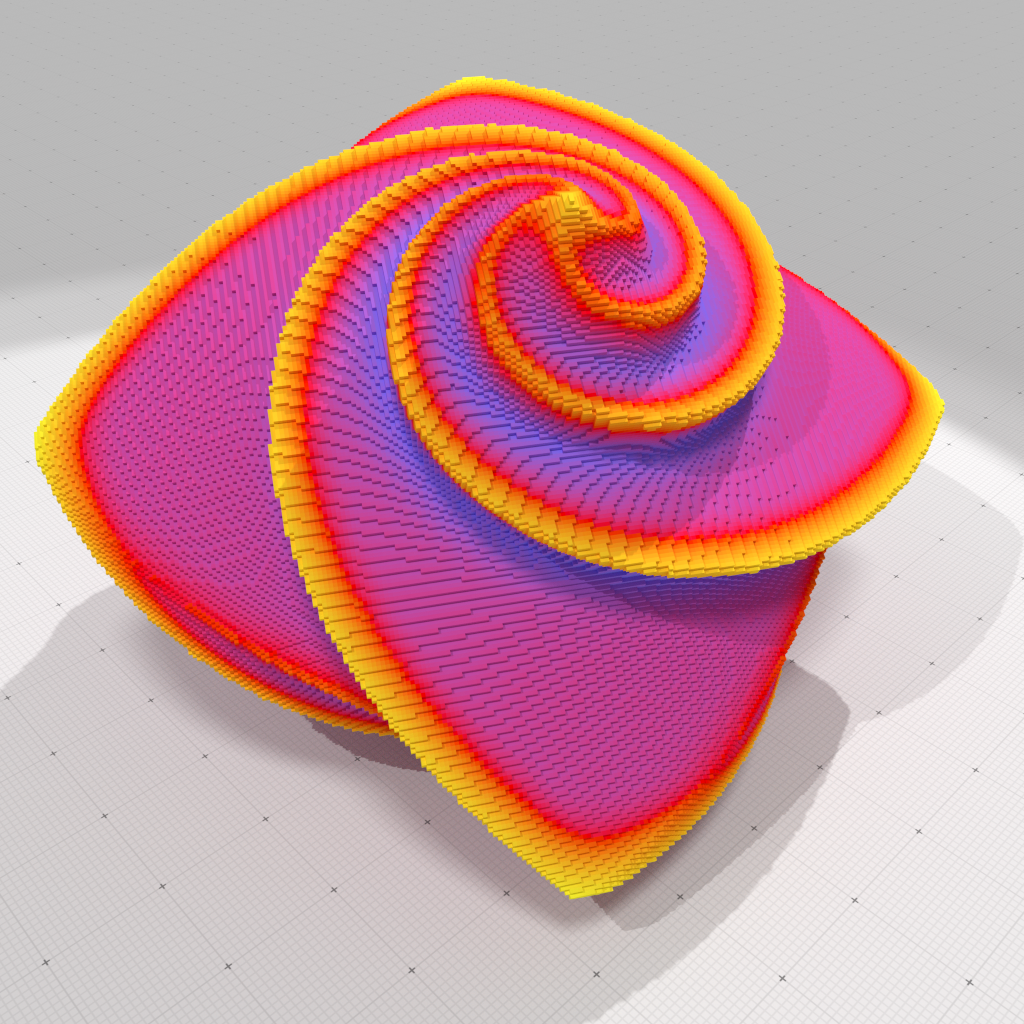
\includegraphics[width=.30\linewidth]{images/Curvature/Octa256_Mean_R_15_0001}
  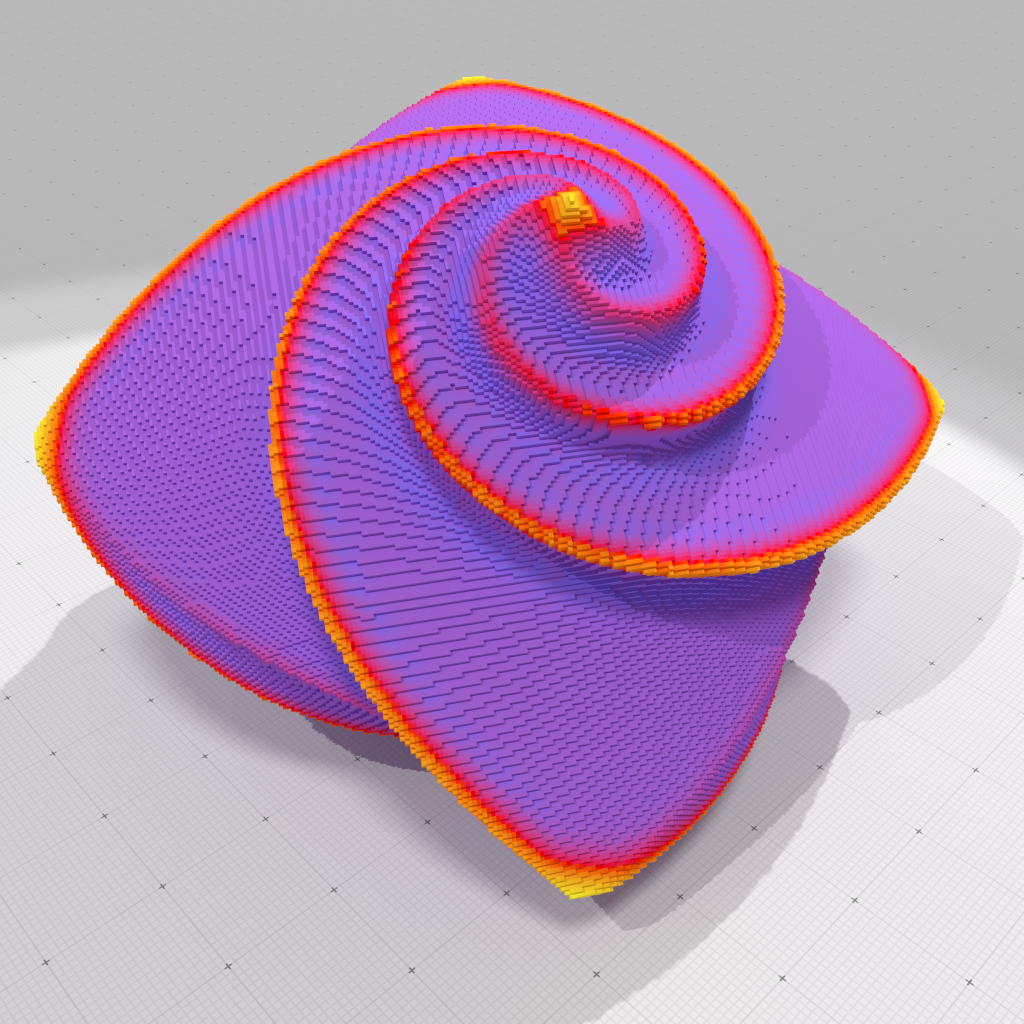
\includegraphics[width=.30\linewidth]{images/Curvature/Octa256_Gauss_R_15_0001}\\
  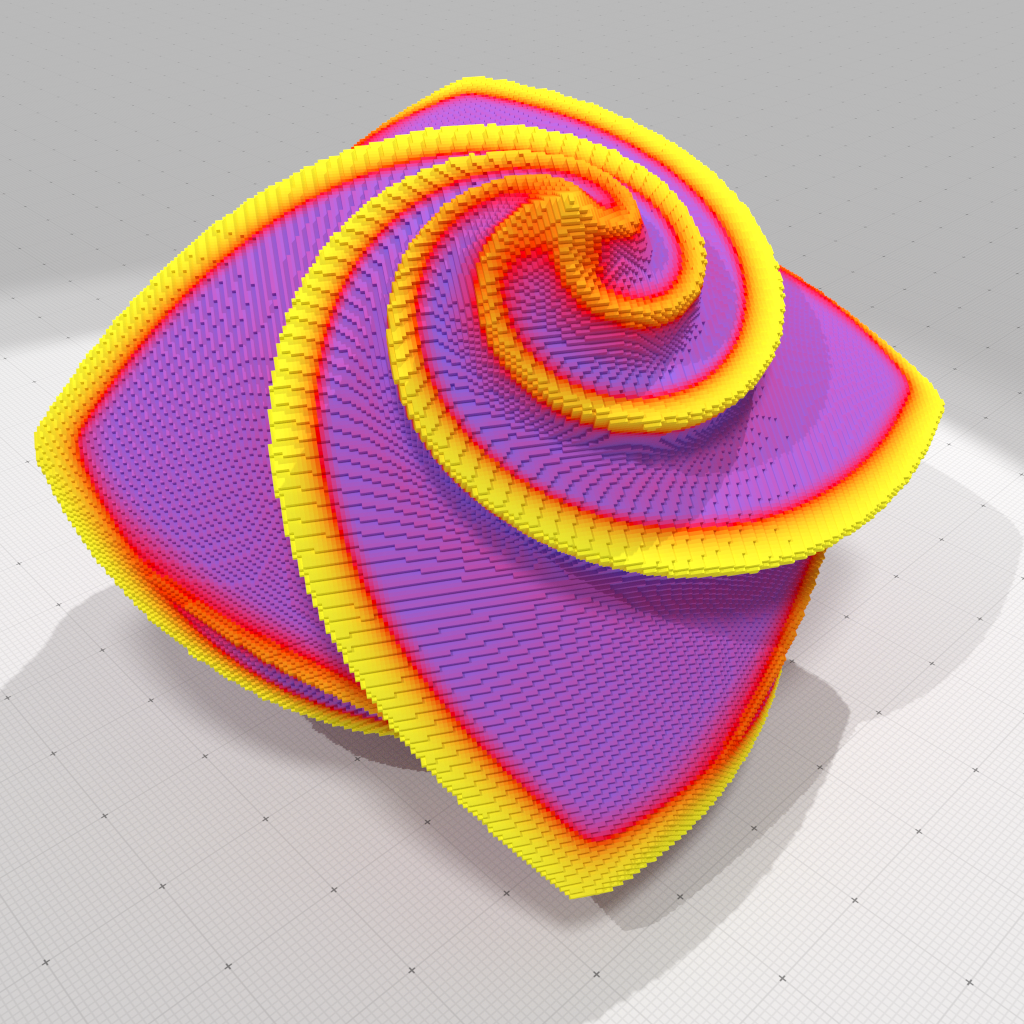
\includegraphics[width=.30\linewidth]{images/Curvature/Octa256_k1_R_15_0001}
  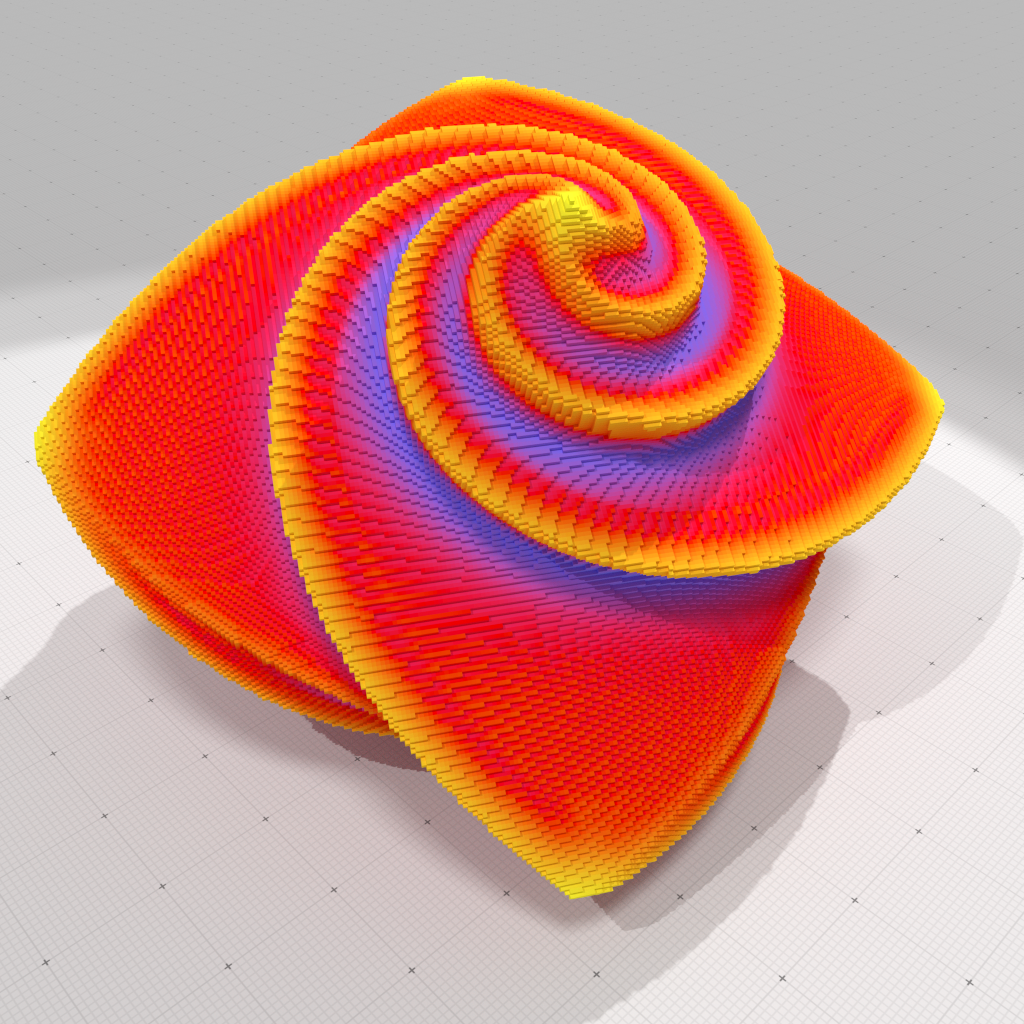
\includegraphics[width=.30\linewidth]{images/Curvature/Octa256_k2_R_15_0001}\\
\end{center}\vspace{-0.5cm}
  \caption[Estimateurs différentiels digitaux par intégration sur une surface digitale (\textsc{OctaFlower} de dimension $256^3$.]{Estimateurs différentiels digitaux par intégration sur une surface digitale (\textsc{OctaFlower} de dimension $256^3$) avec $R = 15$. \emph{De gauche à droite, de haut en bas :} courbure moyenne, courbure gaussienne, première et seconde courbures principales. \label{fig:digital-II-octa}}
\end{figure}

\begin{figure}[ht]
\begin{center}
  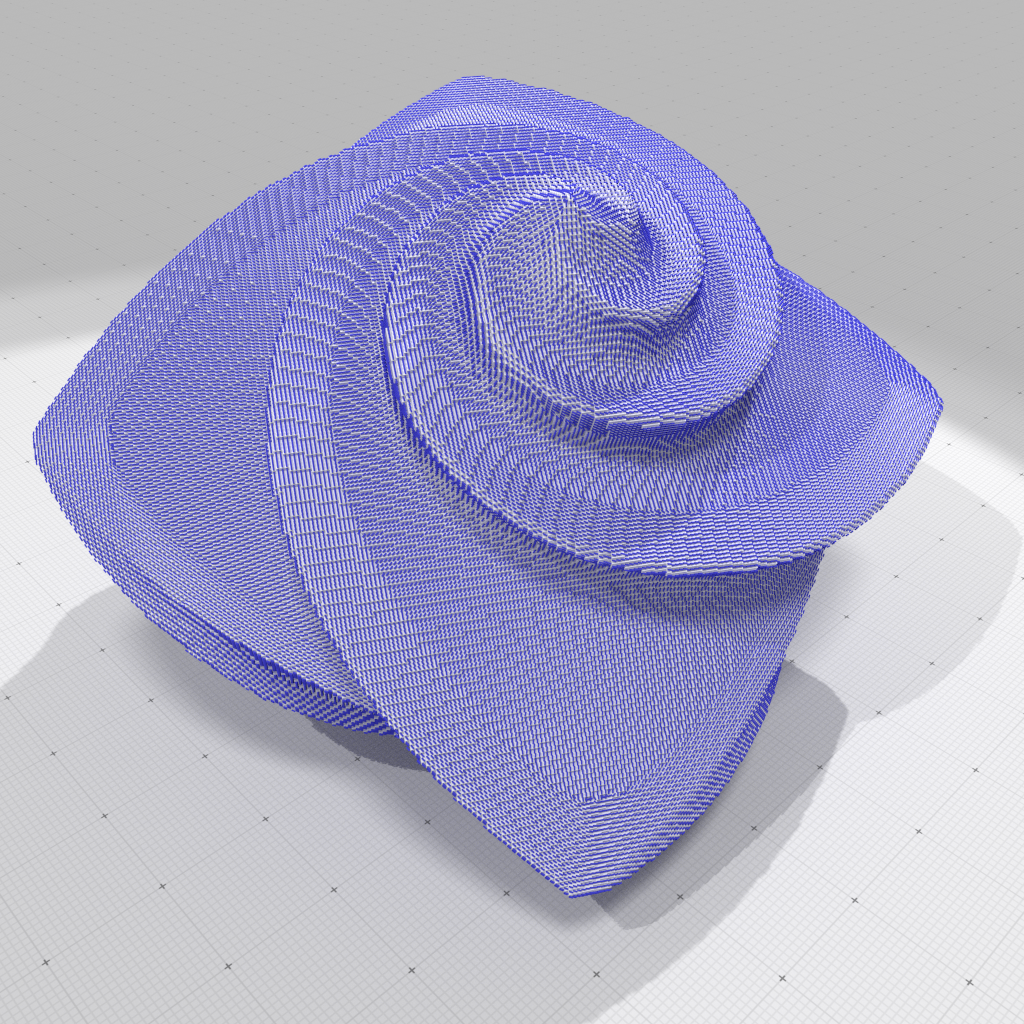
\includegraphics[width=.197\linewidth]{images/Curvature/Octa256_dir1_R_15_0001}
  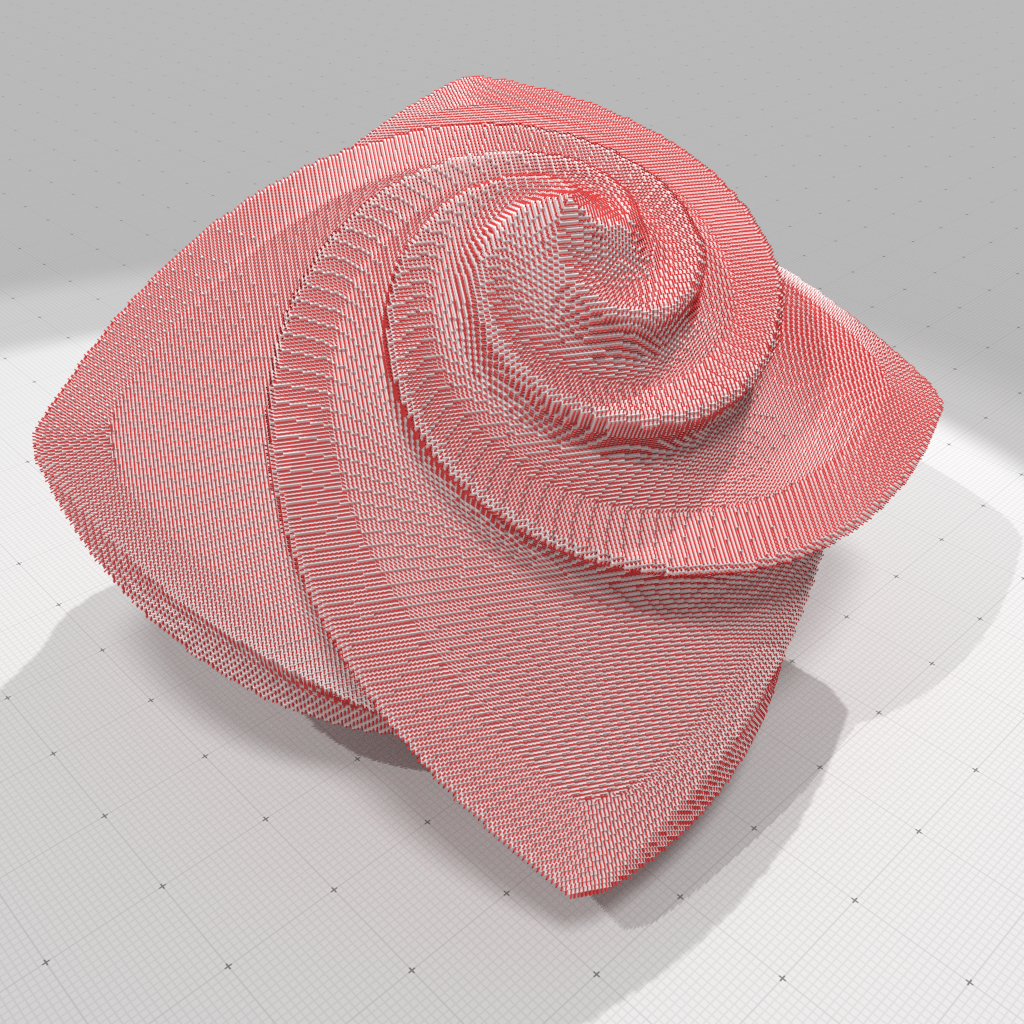
\includegraphics[width=.197\linewidth]{images/Curvature/Octa256_dir2_R_15_0001}
  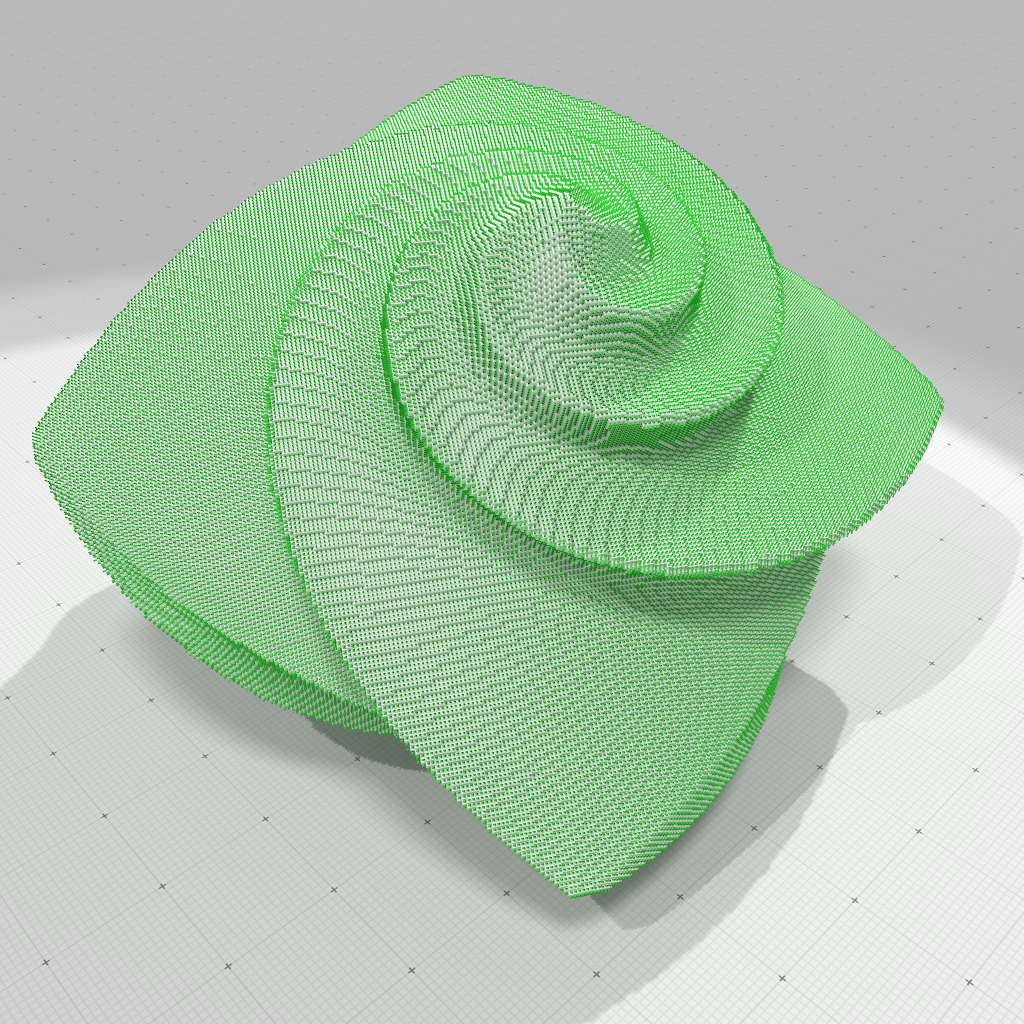
\includegraphics[width=.197\linewidth]{images/Curvature/octa-256-normal}\\
  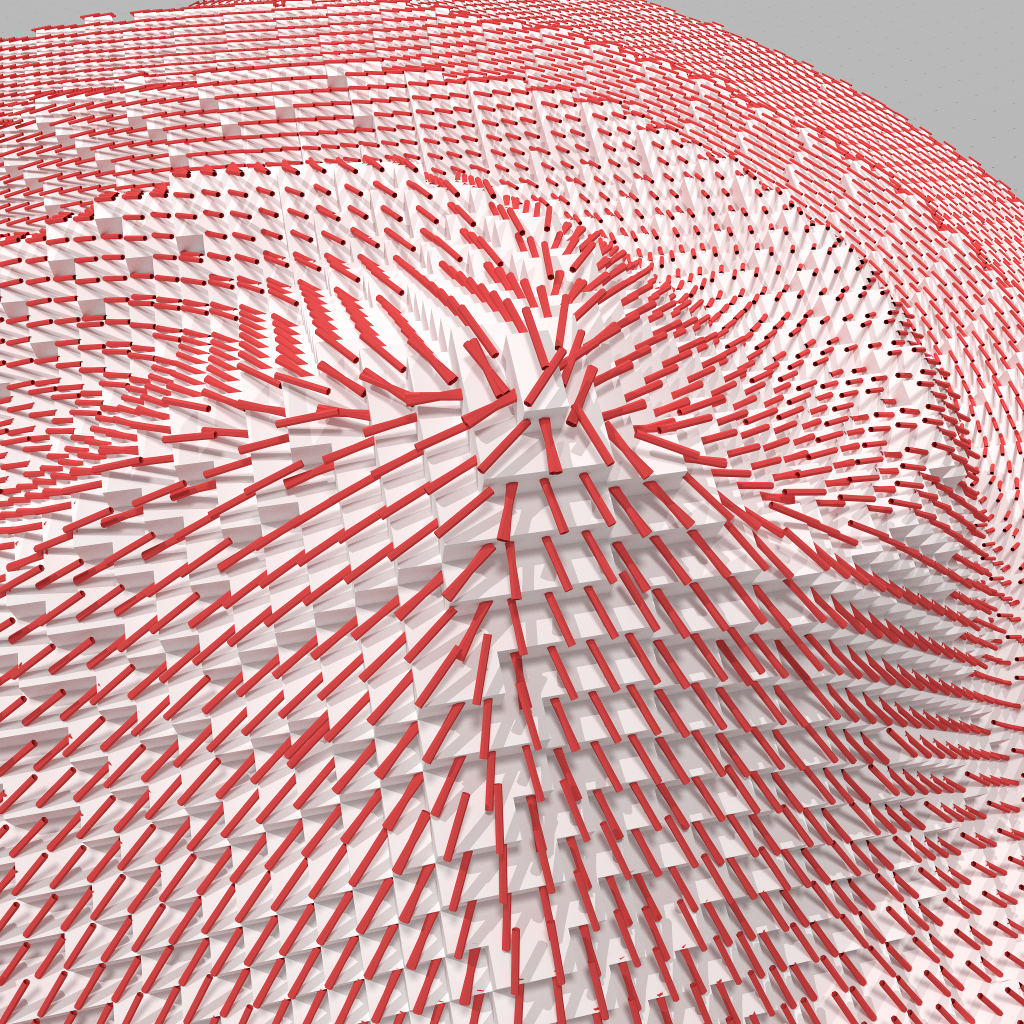
\includegraphics[width=.30\linewidth]{images/Curvature/octa-256-prindir1-zoom}
  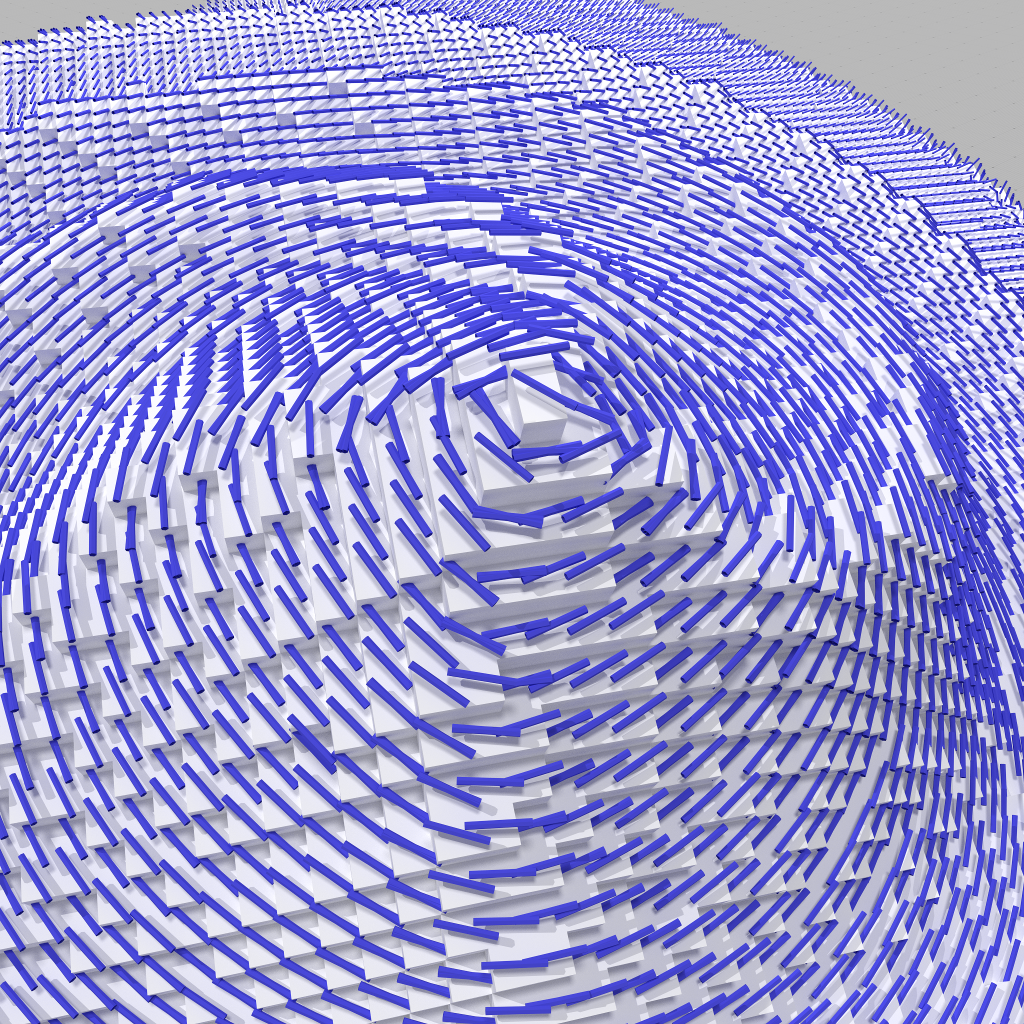
\includegraphics[width=.30\linewidth]{images/Curvature/octa-256-prindir2-zoom}
\end{center}\vspace{-0.5cm}
  \caption[Estimateurs différentiels digitaux par intégration sur une surface digitale (\textsc{OctaFlower} de dimension $256^3$.]{Estimateurs différentiels digitaux par intégration sur une surface digitale (\textsc{OctaFlower} de dimension $256^3$) avec $R = 15$. \emph{De gauche à droite, de haut en bas :} première et seconde direction principale de courbure et normale (zoom sur la dernière ligne). \label{fig:digital-II-octa-2}}
\end{figure}

\section{Estimation sans paramètre de la courbure par intégration volumique de la boule}
\label{sec:curvature:parameter-free}
%
Dans ce paragraphe, nous allons proposer une version sans paramètre des
estimateurs de courbure du \RefSection{sec:estimators:volume}. Dans le contexte
de la convergence asymptotique, la notion d'échelle est explicitement donnée
grâce au paramètre de discrétisation $h$. C'est d'ailleurs pour cela que nos
rayons de boules doivent être en relation avec $h$ ($R$ est en
$O(h^\frac{1}{3})$). Cependant, pour un objet digital donné, ce choix de rayon
nécessite d'étudier au préalable la forme dont nous souhaitons estimer la
courbure, et la qualité d'estimation dépend de ce paramètre. La
\RefFigure{fig:digital-II-octa-scale} montre le résultat de l'estimation de la
courbure moyenne et de la courbure gaussienne avec différents rayons $R$ pour la
forme \textsc{OctaFlower}.

\begin{figure}[ht]
\begin{center}
  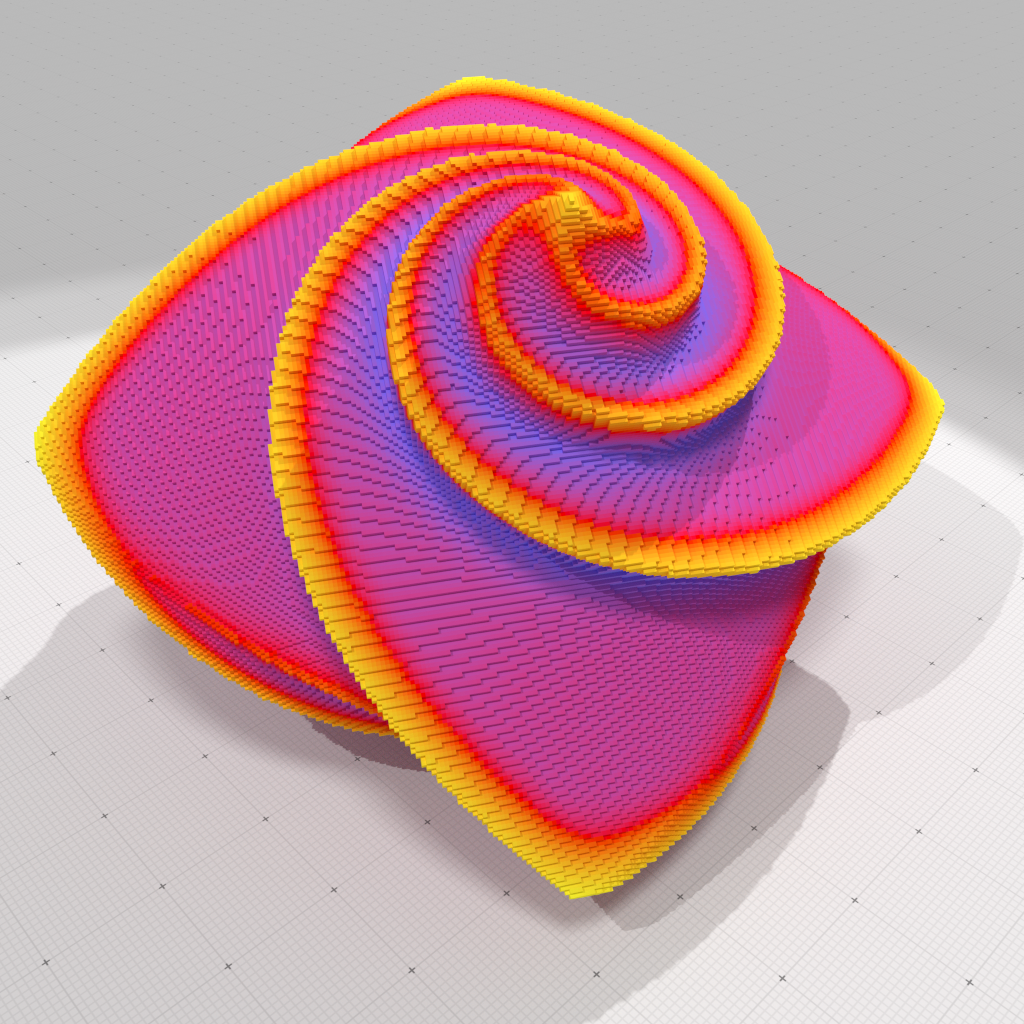
\includegraphics[width=.30\linewidth]{images/Curvature/Octa256_Mean_R_15_0001}
  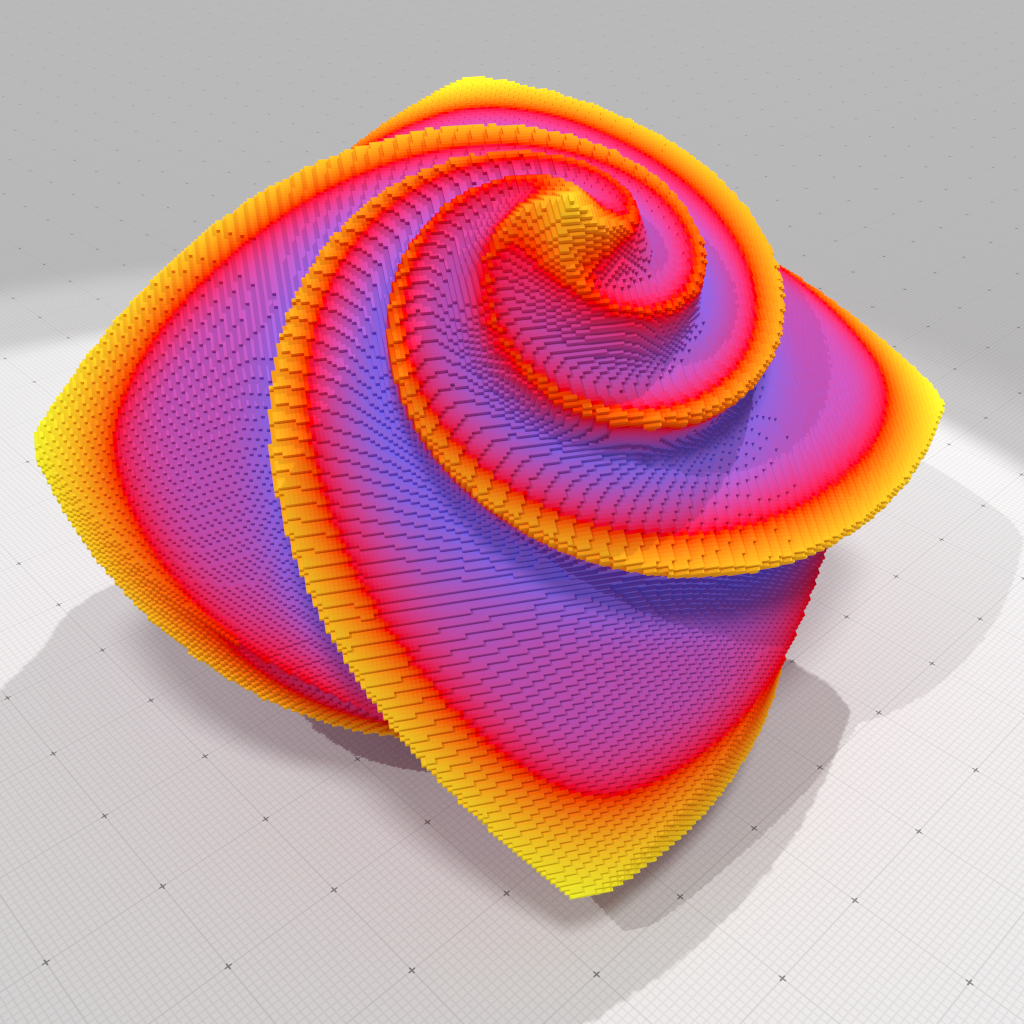
\includegraphics[width=.30\linewidth]{images/Curvature/Octa256_Mean_R_25_0001}
  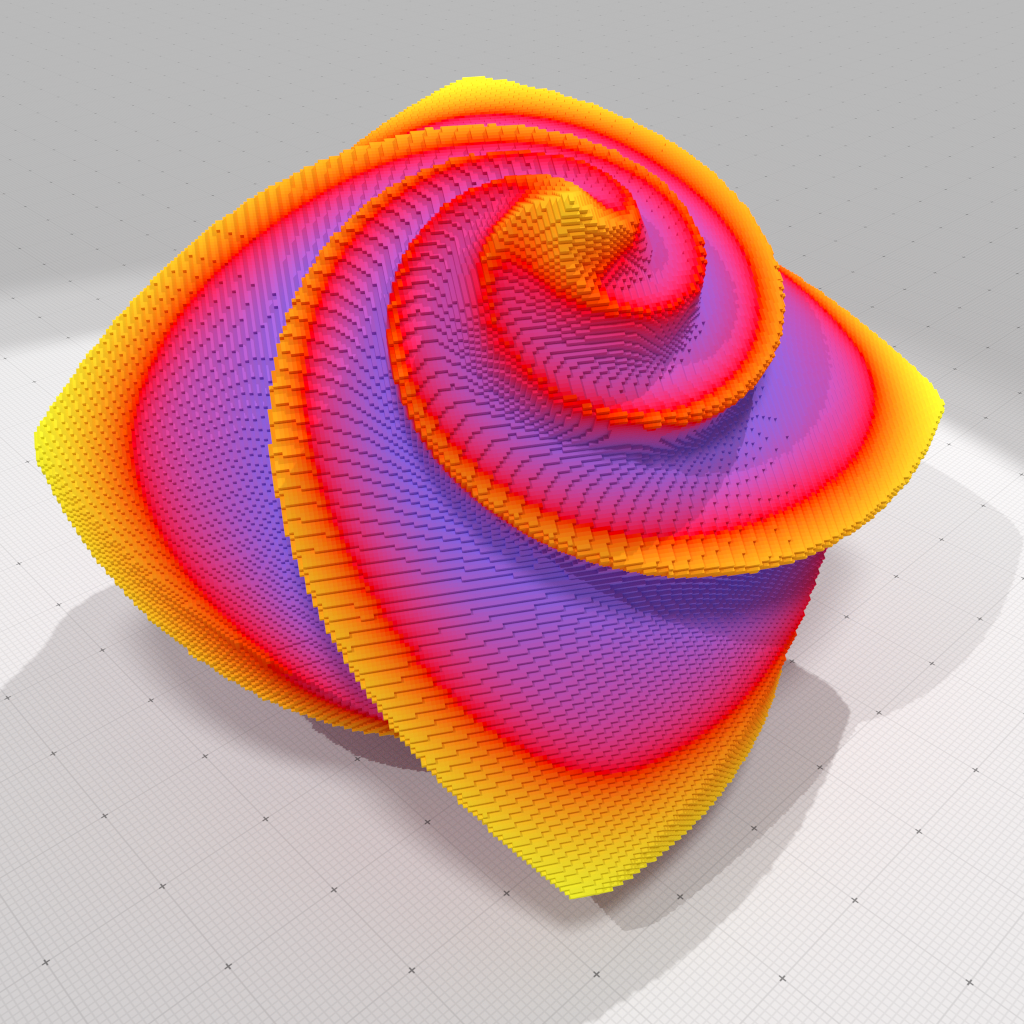
\includegraphics[width=.30\linewidth]{images/Curvature/Octa256_Mean_R_30_0001}\\
  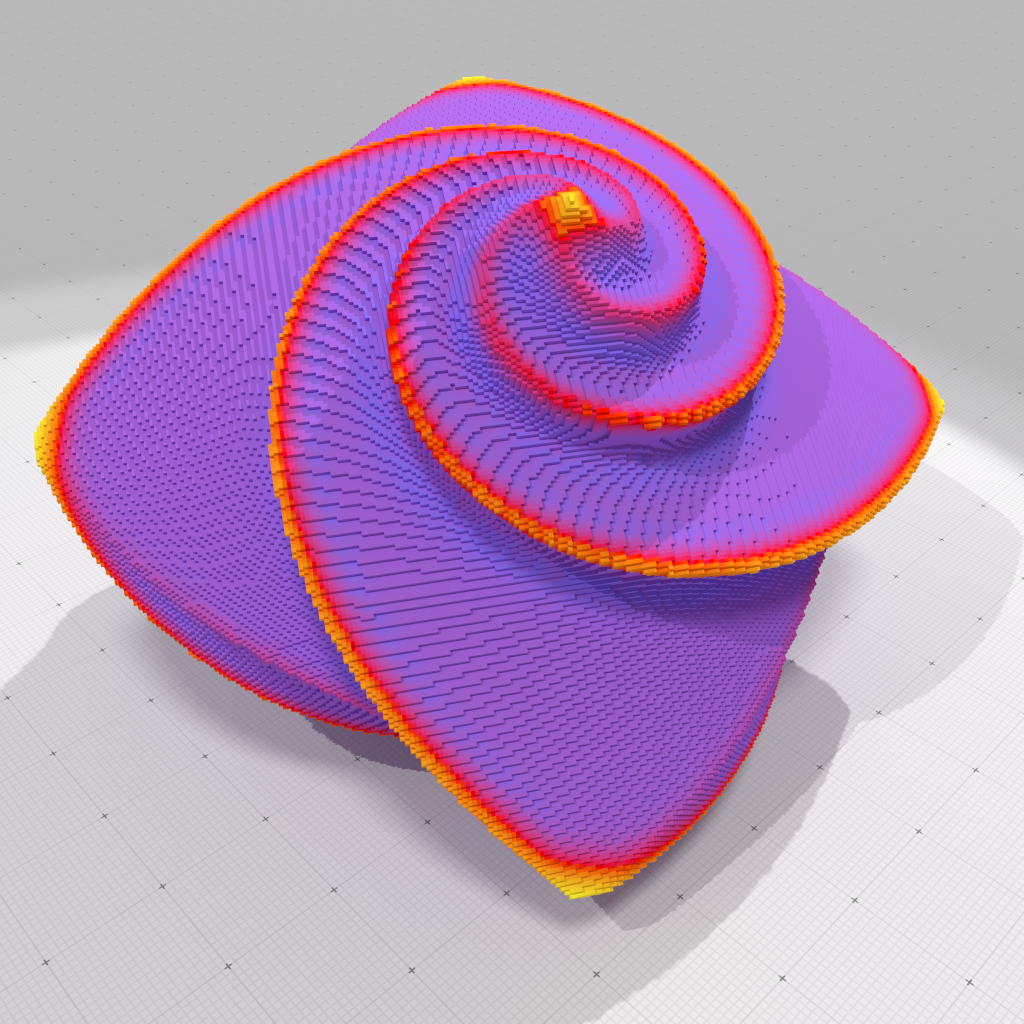
\includegraphics[width=.30\linewidth]{images/Curvature/Octa256_Gauss_R_15_0001}
  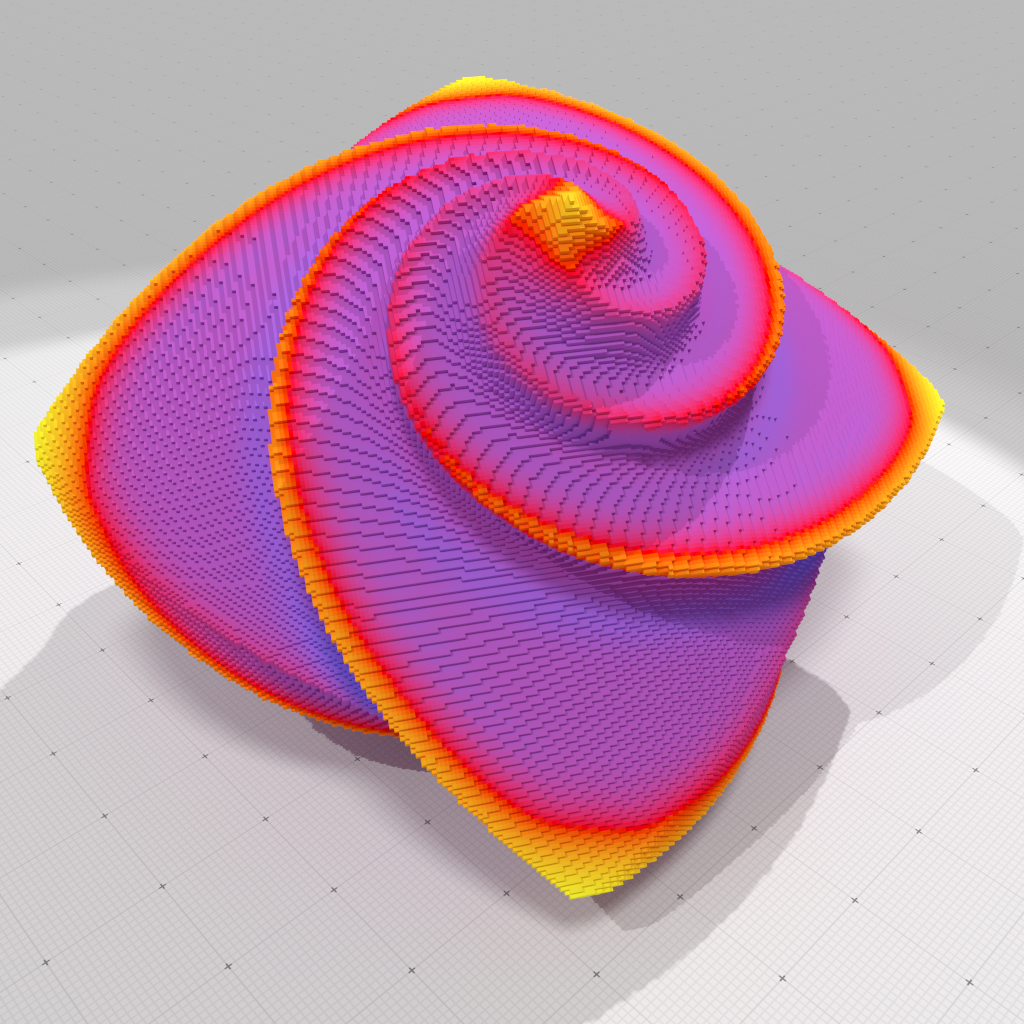
\includegraphics[width=.30\linewidth]{images/Curvature/Octa256_Gauss_R_25_0001}
  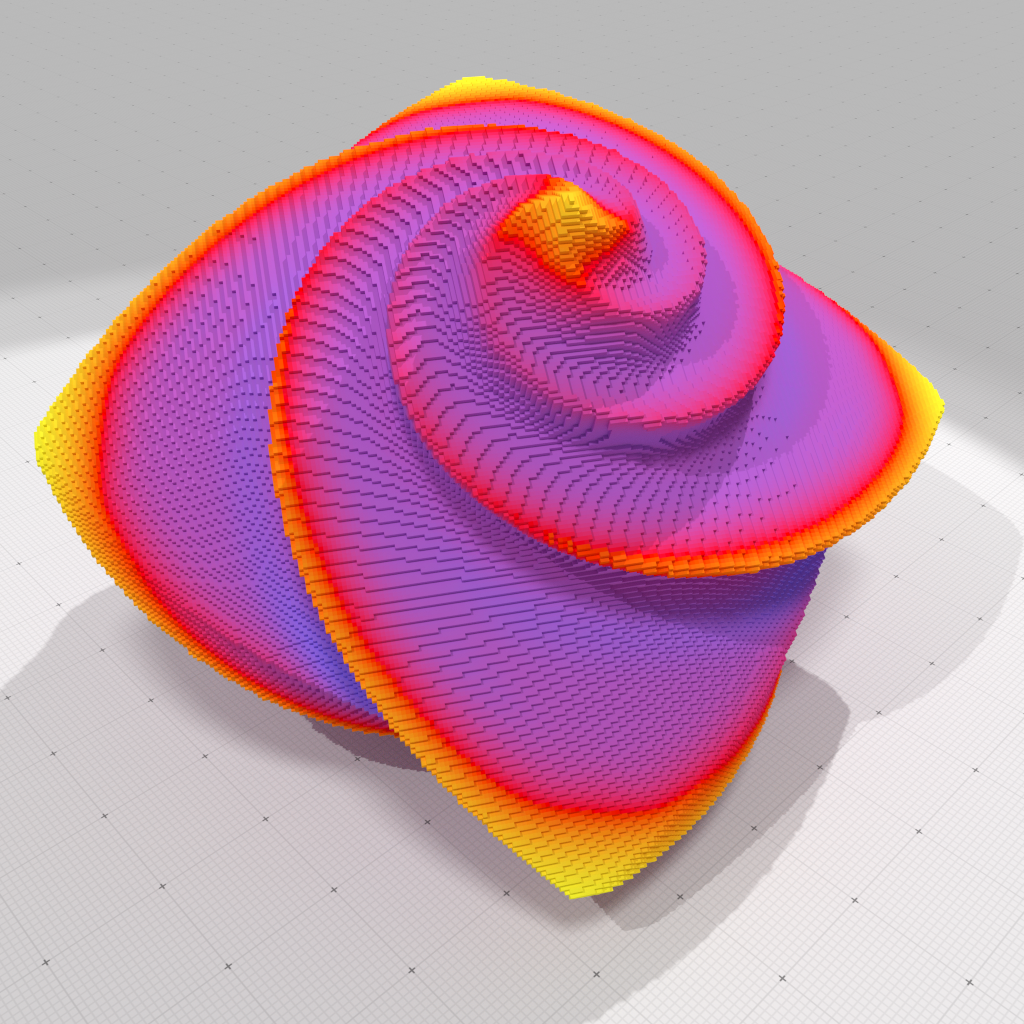
\includegraphics[width=.30\linewidth]{images/Curvature/Octa256_Gauss_R_30_0001}
\end{center}\vspace{-0.5cm}
  \caption{Estimateurs différentiels digitaux par intégration sur une surface digitale (\textsc{OctaFlower} de dimension $256^3$) avec trois rayons différents : $R = 15, 25, 30$. \emph{De haut en bas}, courbure moyenne, courbure gaussienne. \label{fig:digital-II-octa-scale}}
\end{figure}

Nous voulons alors automatiquement détecter ce paramètre de rayon pour des
objets digitaux $\DigShape$ de dimension $2$ et $3$ tout en garantissant les
propriétés de convergence asymptotiques si ceux-ci respectent les conditions de
convergence des estimateurs de courbure du \RefSection{sec:estimators:volume}.
La technique est simple, nous devons extraire les informations géométriques de
la forme afin de pouvoir retrouver quel est le paramètre asymptotique $h$ pour
la forme donnée. Pour ce faire, nous utiliserons les segments maximaux digitaux décris
dans le \RefSection{sec:segments}.
%
%\subsection{Propriétés sur les segments maximaux}
%
\subsection{Estimateur digital sans paramètre de courbure en 2D}
%
Dans le \RefSection{sec:segments} nous avons rappelé les propriétés des longueurs
des segments maximaux sur les bords d'objets digitaux
(\RefLemma{lem:law-length-MDSS}). Nous allons tirer parti de ces propriétés afin
de définir notre nouvel estimateur de courbure sur des objets digitaux
$\DigShape \subset \Z^2$. Pour faire simple, nous allons reprendre l'estimateur
digital de courbure défini dans la \RefDefinition{def:digital-2d-curvature}.
Celui-ci nécessite un rayon $R$ qui doit être en $O(h^{\frac{1}{3}})$ afin
d'avoir une convergence asymptotique de la courbure. Nous allons exploiter les
longueurs des segments maximaux afin de coller à cette
borne\footnote{$L_D({\DigShape})$ est la longueur moyenne des segments maximaux
sur $\DigShape$}. Définissons tout d'abord notre estimateur digital sans
paramètre de courbure en 2D $\CurvHS$ :
%
\begin{definition}
  \label{def:curvature-estimator-2d-pf}
  %
  Soit une forme $\DigShape \subset \Z^2$. L'estimateur digital sans paramètre
  de courbure en 2D $\CurvHS$ au pointel $\vp \in \BdZ{\DigShape}$ est défini comme :
  %
  \begin{equation}
    \CurvHS( \DigShape, \vp) \EqDef \frac{3\pi}{2 \rho(\DigShape)} - \frac{3 A(\DigShape,\vp)}{{\rho(\DigShape)}^3}
  \end{equation}
  %
  où $\rho(\DigShape) =L_D^2(\DigShape)$ et $A(\DigShape,\vp) =
  Card(\Ball{\rho(\DigShape)}{\vp} \cap \DigShape)$.
  %
\end{definition}
%
Pour paraphraser cette définition, nous devons dans un premier temps calculer la
moyenne des longueurs des segments discret sur le bord de $\DigShape$. Nous
élevons au carré cette longueur moyenne afin de donner $\rho$. Ainsi,
l'estimateur $\CurvHS$ est une fonction du nombre de points digitaux de
$\DigShape$ intersecté avec une boule de rayon $\rho$ centrée au point digital
$\vp$. Cette version de l'estimateur de la
\RefDefinition{def:digital-2d-curvature} est alors indépendant de l’échelle de la
forme.


Si nous souhaitons rendre compatible notre estimateur dans le cadre de la
convergence asymptotique, afin qu'il puisse se comparer avec des données de
l'espace euclidien, nous devons y appliquer un facteur d'échelle du pas de
discrétisation $h$. En effet, comme nous l'avons dit précédemment, notre
estimateur ne contient pas d'information d'échelle. De plus, pour $\DigShape =
\DSh$, avec $\rho(\DigShape) = L^2_D(\DigShape)$, nous avons (d'après le
\RefLemma{lem:law-length-MDSS}) :
%
\begin{align}
  \Theta(h^{-\frac{1}{3}}) \le L_D( \DigShape ) \le \Theta(h^{-\frac{1}{3}} \log \left(\frac{1}{h}\right)) \\
  \Theta(h^{-\frac{2}{3}}) \le L^2_D( \DigShape ) \le \Theta(h^{-\frac{2}{3}} \log^2 \left(\frac{1}{h}\right)) \\
  \Theta(h^{\frac{1}{3}}) \le hL^2_D( \DigShape ) \le \Theta(h^{\frac{1}{3}} \log^2 \left(\frac{1}{h}\right)) \label{eq:bounds-length-MDSS}.
\end{align}
%


Ainsi, à l'exception du terme en $\log^2(\cdot)$, $h \rho(\DigShape)$ semble est
un candidat parfait comme paramètre de rayon $R$, puisqu'il suit
approximativement $\Theta(h^\frac{1}{3})$, pour obtenir un estimateur digital
sans paramètre de courbure.
%
\begin{theorem}{\fakeTitle{Convergence asymptotique de l'estimateur digital de courbure sans paramètre $\CurvHS$}}
\label{thm:curvature-estimator-2d-pf-conv}
  %
  Soit $\Shape$ une forme convexe de $\R^2$ telle que son bord $\Bd{\Shape}$ est
  $C^3$ et sa courbure bornée non nulle. Soit $\DigShape = \DSh$. Alors, avec une
  constante positive $h_0$, nous avons :
  %
  \begin{align}
    &\forall 0 < h \le h_0, \quad \forall \vx \in \dS, \quad \forall \vp \in \BdZ{\DigShape} \text{~avec~} \| h\vp -\vx\|_\infty \le h, \nonumber\\
    &\left | \frac{1}{h}\CurvHS(\DigShape,\vp) - \Curv(\Shape,\vx) \right| \le O\left( h^{\frac{1}{3}} \log^2 \left(\frac{1}{h}\right)\right) .
    %
  \end{align}
  %
\end{theorem}
%
Il est à noter que $\vp \in \BdZ{\DigShape}$ implique que $h\vp \in
\Bd{\Body{\DSh}{h}}$.


\begin{proof}
  %
  Dans un premier temps, nous allons décomposer
  $\frac{1}{h}\CurvHS(\DigShape,\vp)$ :
  %
  \begin{align}
    \frac{1}{h}\CurvHS(\DigShape,\vp) &= \frac{3\pi}{2 h\rho(\DigShape)} - \frac{3 A(\DigShape,\vp)}{h{\rho(\DigShape)}^3} \\
    &= \frac{3\pi}{2 h\rho(\DigShape)} - \frac{3~ Card(\Ball{\rho(\DigShape)}{\vp} \cap \DSh)}{h{\rho(\DigShape)}^3} \\
    &= \frac{3\pi}{2 h\rho(\DigShape)} - \frac{3~ Card( \Ball{(h\rho(\DigShape))/h}{\frac{1}{h} \cdot (h\vp)} \cap \DSh, h)}{h{\rho(\DigShape)}^3} \\
    &= \CurvH{R}(\DSh,\hat{\vx},h)\quad \text{(avec $R \EqDef h\rho(\DigShape)$ et $\hat{\vx} \EqDef h\vp$)}
  \end{align}
  %
  Il suffit alors de simplement borner $| \CurvH{R}(\DSh,\hat{\vx},h) -
  \Curv(\DSh,\vx) |$ en tenant compte du comportement asymptotique de $R \EqDef
  h\rho(\DigShape)$. D'après l'\RefEquation{eq:bounds-length-MDSS}, $r$ est
  compris entre deux bornes :
  \begin{itemize}
    %
    \item Si $R = \Theta(h^{\frac{1}{3}})$, nous sommes exactement dans les
    hypothèses du \RefTheorem{thm:convergence-curv-2d}, alors le terme d'erreur
    est en $O( h^\frac{1}{3} )$.
    %
    \item Si $R = \Theta(h^{\frac{1}{3}} \log^2 \left(\frac{1}{h}\right))$, nous
    décomposons le terme d'erreur du \RefTheorem{thm:convergence-curv-2d} en
    utilisant l'\RefEquation{eq:shift-curvhat-error-bound-h-only}\footnote{En
    tenant compte que $\alpha' = 1$ et $\beta = 1$ dans le cas général} :
    %
    \begin{align}
      |\CurvH{R}(\DSh,\hat{\vx},h) - \Curv(\Shape,\vx)| & \le O(h\rho(\DigShape)) + O\left(\frac{h}{(h\rho(\DigShape))^{2}}\right) \nonumber\\
      &\quad + O\left(\frac{h}{(h\rho(\DigShape))^{2}}\right)( 1 + O((h\rho(\DigShape))^2) + O(h)) \\
      & \le O(h^{\frac{1}{3}} \log^2 (\frac{1}{h})) + O\left(\frac{h^\frac{1}{3}}{\log^4 (\frac{1}{h})}\right) + O( h ) \nonumber\\
      &\quad + O\left(\frac{h^\frac{4}{3}}{\log^4 (\frac{1}{h})}\right)
    \end{align}
    %
    Alors le terme d'erreur dominant de cette expression est $O(h^{\frac{1}{3}}
    \log^2 (\frac{1}{h}))$
    %
  \end{itemize}
  %
  Ainsi, nous allons borner par le terme d'erreur dominant des deux
  possibilités. Puisque
  $\frac{1}{h}\CurvHS(\DigShape,\vp)=\CurvH{R}(\DSh,\hat{\vx},h)$, nous pouvons
  conclure que son erreur est en $O(h^{\frac{1}{3}} \log^2 (\frac{1}{h}))$
  %
\end{proof}


De ce fait, nous avons un estimateur digital de courbure qui converge, qui ne
nécessite aucun paramètre de rayon. Le paramètre d'échelle $h$ est présent
seulement pour déterminer l'unité utilisée pour mesurer les courbures comme
l'explique la \RefFigure{fig:2d-parameter-free-explained}.

\begin{figure}[ht]
  \begin{center}
    
\begin{tikzpicture}[x=0.50cm,y=0.50cm]
  % colors
  \definecolor{kGreen}{rgb}{0.0,0.59,0.0}
  \definecolor{kOrange}{rgb}{1.0,0.59,0.0}
  \definecolor{kGrey}{rgb}{0.33,0.33,0.33}
  % grids
  \draw[help lines,step=1] (0,0) grid (10,10);
  \node (px) at (5,5) {};
  \draw[draw,thick,fill,color=kOrange,nearly transparent] (px) circle (3);
  \draw[draw,thick,color=kOrange] (px) circle (3);
  \foreach \x/\y in {2/5, 3/3, 3/4, 3/5, 3/6, 3/7, 4/3, 4/4, 4/5, 4/6, 4/7, 5/2, 5/3, 5/4, 5/5, 5/6, 5/7, 5/8, 6/3, 6/4, 6/5, 6/6, 6/7, 7/3, 7/4, 7/5, 7/6, 7/7, 8/5}
    \draw[draw,thick,color=kGrey,fill] (\x,\y) circle (0.1);
\end{tikzpicture}
\begin{tikzpicture}[x=0.50cm,y=0.50cm]
  % colors
  \definecolor{kGreen}{rgb}{0.0,0.59,0.0}
  \definecolor{kOrange}{rgb}{1.0,0.59,0.0}
  \definecolor{kGrey}{rgb}{0.33,0.33,0.33}
  % grids
  \draw[help lines,step=0.5] (0,0) grid (10,10);
  \node (px) at (5,5) {};
  \draw[draw,thick,fill,color=kOrange,nearly transparent] (px) circle (1.5);
  \draw[draw,thick,color=kOrange] (px) circle (1.5);
  \foreach \x/\y in {3.5/5, 4/4, 4/4.5, 4/5, 4/5.5, 4/6, 4.5/4, 4.5/4.5, 4.5/5, 4.5/5.5, 4.5/6, 5/3.5, 5/4, 5/4.5, 5/5, 5/5.5, 5/6, 5/6.5, 5.5/4, 5.5/4.5, 5.5/5, 5.5/5.5, 5.5/6, 6/4, 6/4.5, 6/5, 6/5.5, 6/6, 6.5/5}
    \draw[draw,thick,color=kGrey,fill] (\x,\y) circle (0.05);
\end{tikzpicture}

  \end{center}
  \caption[Illustration de la dépendance du paramètre d'échelle $h$.]
  %
  {Illustration de la dépendance du paramètre d'échelle $h$. L'objet euclidien
  de gauche donne le même objet digital que l'objet euclidien de droite alors
  qu'ils sont à des échelles différentes. La courbure à la surface de l'objet
  dépend alors de $h$.\label{fig:2d-parameter-free-explained}}
  %
\end{figure}

Nous utilisons un unique rayon pour estimer la courbure sur tout le bord de
l'objet. En sachant que nous pouvons extraire des faisceaux de segments maximaux
en chaque point du bord de l'objet, pouvons-nous adapter notre estimateur afin
de la taille de la boule s'adapte localement à la géométrie de l'objet ? Le
paragraphe suivant traite cette question.
%
\subsection{Estimateur digital local sans paramètre de courbure en 2D}
%
Nous allons noter $\rho(\DigShape,\vp)$ la longueur moyenne du faisceau de
segments maximaux au point $\vp$ élevé au carré. Nous définissons alors une
version locale de l'estimateur de la
\RefDefinition{def:curvature-estimator-2d-pf} :
%
\begin{definition}
  %
  Soit une forme $\DigShape \subset \Z^2$. L'estimateur digital local sans
  paramètre de courbure en 2D au pointel $\vp \in \BdZ{\DigShape}$ est défini par :
  %
  \begin{equation}
    \CurvHSL(\DigShape, \vp) \EqDef \frac{3\pi}{2 \rho(\DigShape,\vp)} - \frac{3 A'(\DigShape,\vp)}{{\rho(\DigShape,\vp)}^3}
  \end{equation}
  %
  où $A'(\DigShape, \vp) = Card(\Ball{\rho(\DigShape,\vp)}{\vp} \cap
  \DigShape)$.
  %
\end{definition}
%
Pour résumer, nous calculons le faisceau de segments maximaux en tout point
$\vp$ du bord de $\DigShape$, puis nous calculons la moyenne de leurs longueurs.
Cette longueur au carré nous donne la taille à utiliser pour la boule localement
pour le point $\vp$. La conséquence de ceci est d'avoir une plus grosse boule
sur les parties à faible courbure et de diminuer la taille de la boule sur les
zones fortement courbées. La \RefFigure{fig:curvature-pf-radii} montre la
différence entre $\CurvHS$ et $\CurvHSL$ : dans sa version locale, le rayon est
adapté localement à la géométrie de la forme.

\begin{figure}[ht]{
  \begin{center}
    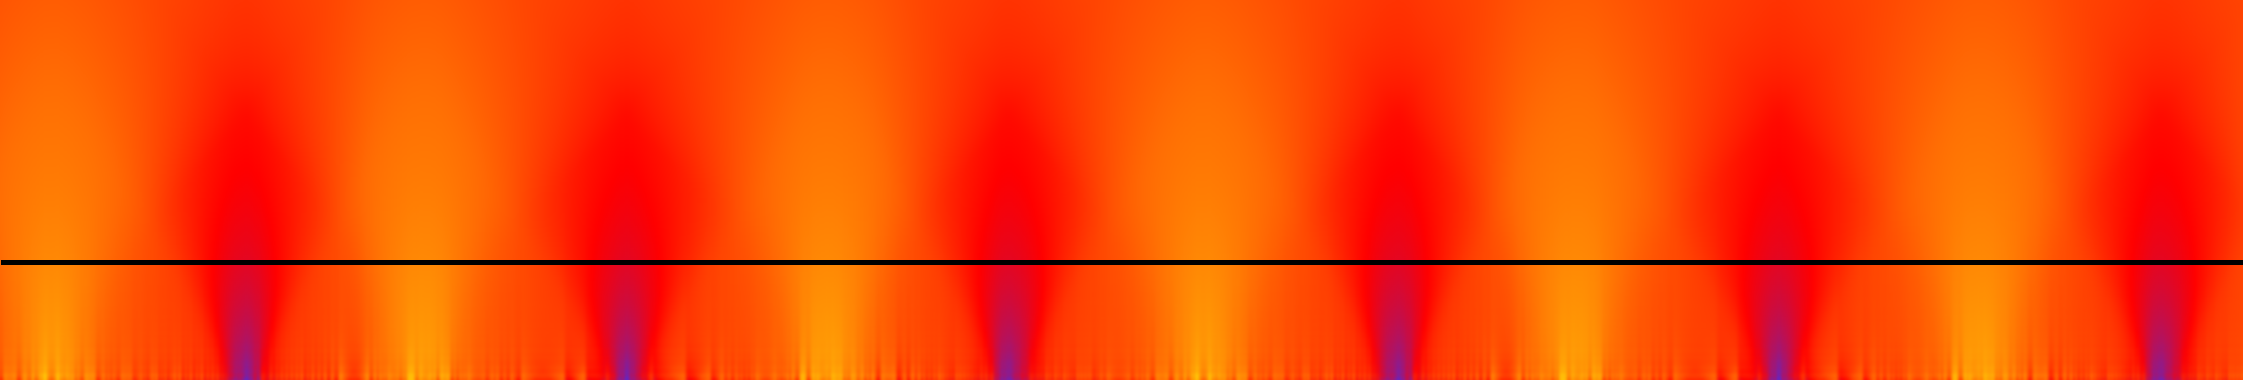
\includegraphics[width=.95\linewidth]{images/Curvature/ScaleSpace_Flower_Global}
    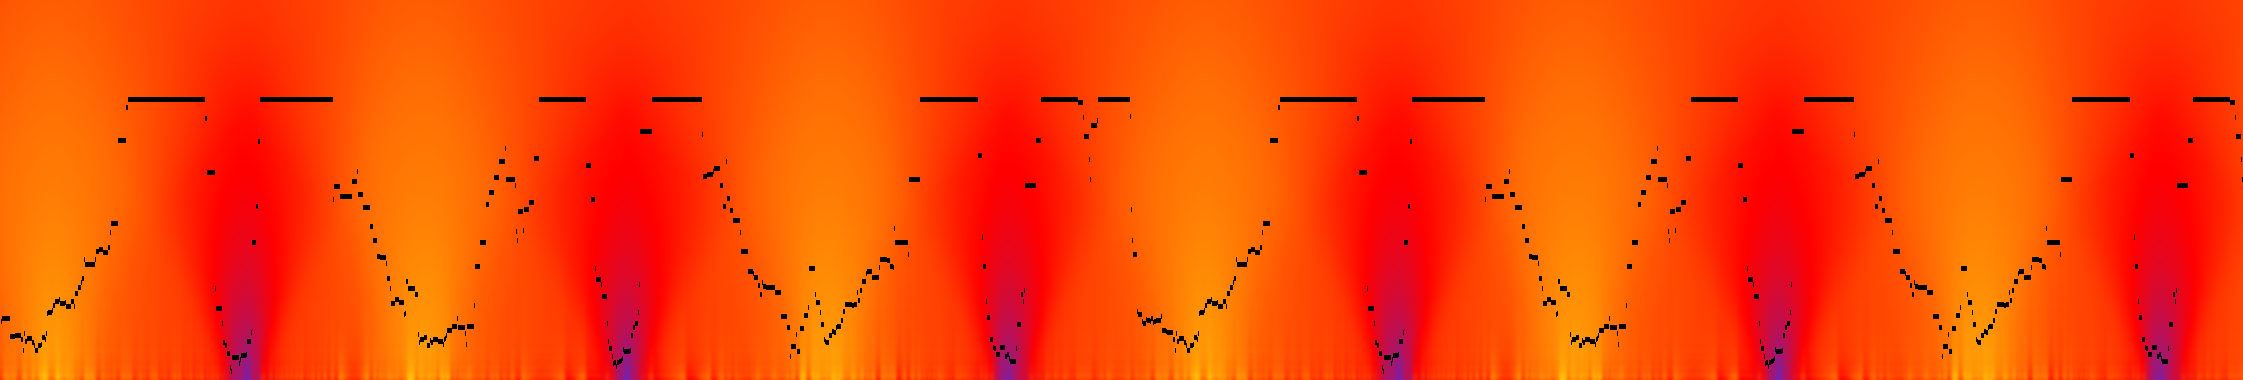
\includegraphics[width=.95\linewidth]{images/Curvature/ScaleSpace_Flower_Local}
    %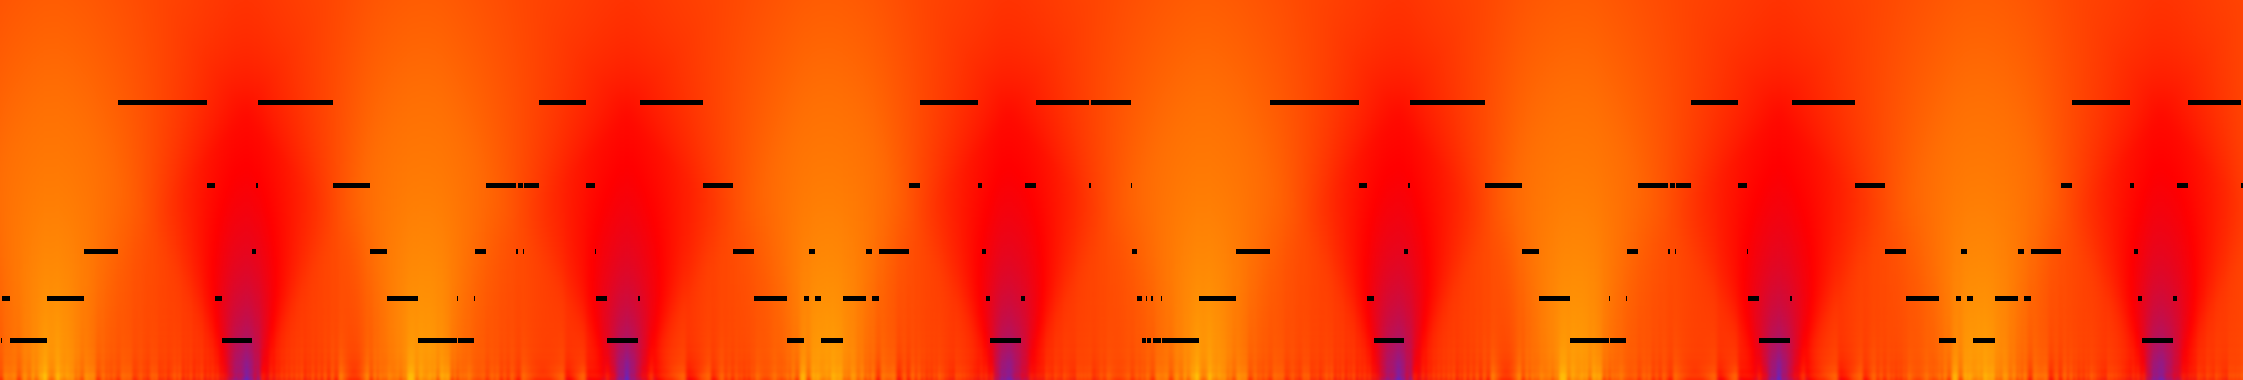
\includegraphics[width=.95\linewidth]{images/Curvature/ScaleSpace_Flower_Local_5}
  \end{center}}
  %
  \caption{Valeur de courbure estimée en fonction du rayon $R$ sur le bord de
  l'objet \textsc{AccFlower} allant du bleu (valeur minimale) au jaune (valeur
  maximale). \emph{En abscisse :} position sur la surface de l'objet, \emph{en
  ordonnée :} différents rayons $R$.
  %
  \\
  %
  \emph{En noir sur l'image du haut :} rayon choisi par l'estimateur $\CurvHS$.
  \emph{En noir sur l'image du bas :} différents rayons choisis par l'estimateur
  $\CurvHSL$ en fonction de la géométrie locale de la forme.
  %
  \label{fig:curvature-pf-radii}}
  %
\end{figure}

Dans cette version locale, quelques segments maximaux peuvent avoir une longueur
trop importante, ce qui nous empêche d'obtenir des preuves de convergence
asymptotique. En effet, si, dans le faisceau de segments maximaux, les longueurs
sont globalement dans l'intervalle $\Theta(h^{-\frac{1}{3}}) \le L_D(
{\DigShape} ) \le \Theta(h^{-\frac{1}{3}} \log \left(\frac{1}{h}\right))$, un
bon comportement asymptotique peut être envisagé pour cet estimateur local.
Cependant, des problèmes interviennent avec les segments maximaux les plus long : à
cause de leur borne supérieur en $O(h^{-\frac{1}{2}})$ aucune convergence ne peut
être espérée. Néanmoins, l'évaluation expérimentale (voir
\RefSection{sec:comparaison-courbure}) montre de bonnes propriétés de
convergence asymptotique et nous pouvons observer que la version locale
$\CurvHSL$ est plus performante que $\CurvHS$.
%
\subsection{Estimateur digital sans paramètre de courbures en 3D}
%
Intéressons nous maintenant à la version en 3D de ces estimateurs sans paramètre.
Nous devons adapter l'utilisation des longueurs des segments maximaux à des
objets $\DigShape \subset \Z^3$. Comme le montre la
\RefFigure{fig:3d-dig-object-slices}, nous proposons d'utiliser des coupes de
l’objet afin d'extraire des contours 2D, et ainsi pouvoir calculer les segments
maximaux.

\begin{figure}[ht]
    \begin{center}
      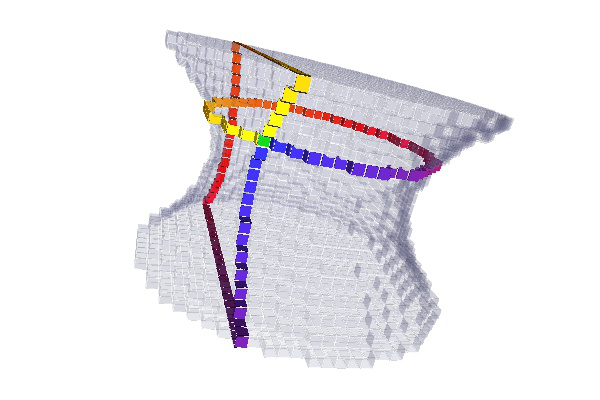
\includegraphics[width=6cm]{images/Curvature/ctopo3dSurfelCut}
    \end{center}
    \caption[Coupes sur un objet digital 3D.]{Coupes sur un objet digital 3D dans deux directions.}
    \label{fig:3d-dig-object-slices}
\end{figure}

Formalisons cela avec une proposition sur les variétés lisses :
%
\begin{proposition}
\label{prop:slices-3d}
  %
  Soit un objet $\Shape \subset \R^3$ avec un bord $C^2$ auquel la valeur
  absolue des courbures principales (notées respectivement $\PrincCurv{1}$ et
  $\PrincCurv{2}$) est bornée par une constante $K$. La normale de $\dS$ au
  point $\vx$ est notée $\vec{\NormalDir}(\vx)$. Pour tout $\vx \in \dS$, on
  considère le plan $\pi_{\vec{\ve}}(\vx)$ contenant $\vx$ et perpendiculaire à
  un vecteur canonique $\vec{\ve}$ de la base de $\R^3$ (\emph{i.e.}
  $\vec{\ve}\in\{ \vec{\vx}_1, \vec{\vx}_2, \vec{\vx}_3 \}$).
  %
  \\
  %
  Soit $\dS_{\vec{\ve}}(\vx)$ le bord de l'intersection $\Shape
  \cap \pi_{\vec{\ve}}(\vx)$. Alors, il y a \textbf{au moins} deux ensembles parmi
  $\dS_{\vec{\vx}_1}(\vx)$, $\dS_{\vec{\vx}_2}(\vx)$ et
  $\dS_{\vec{\vx}_3}(\vx)$ qui sont localement des courbes dont la
  courbure est bornée par $\sqrt{2}K$ en valeur absolue.
  %
\end{proposition}
\begin{proof}
  %
  Afin d'alléger la lecture, nous avons retiré les $(\vx)$ de toutes les
  notations puisqu'il ne peut y avoir d’ambiguïté. La
  \RefFigure{fig:slices-3d-proof} illustre les notations utilisées.
  %
  \begin{figure}[ht]
    \begin{center}
      \begin{overpic}[width=10cm]{figures/Slice_3D}
      \put(40.5,48){$\pi_{\vec{\vx}_2}$}
      \put(95,50){$\pi_{\vec{\vx}_2}$}

      \put(53,19.5){$\dS$}

      \put(33,26){$\vx$}
      \put(80,30){$\vx$}

      \put(5,22.5){$\textcolor{blue}{\gamma_{\PrincCurv{2}}}$}
      \put(36,10){$\textcolor{blue}{\gamma_{\PrincCurv{1}}}$}

      \put(69,27){$\gamma$}
      \put(23,15){$\gamma$}

      \definecolor{darkgreen}{rgb}{0.,0.7,0.}

      \put(29,8){\textcolor{darkgreen}{$\chi$}}
      \put(31,43){\textcolor{darkgreen}{$\pi_{\vec{\NormalDir} \times \vec{\vt}}$}}

      \put(24,33){$\textcolor{red}{\vec{\NormalDir}}$}

      \put(33,35){$\textcolor{darkgreen}{\vec{\vt}(0)}$}
      \put(85,30){$\textcolor{darkgreen}{\vec{\vt}(0)}$}
      \put(80,24){$\textcolor{black}{\vec{\vu}}$}

      \put(52,48){$\textcolor{gray}{\vec{\vx}_1}$}
      \put(51.5,44){$\textcolor{gray}{\vec{\vx}_2}$}
      \put(47,51.5){$\textcolor{gray}{\vec{\vx}_3}$}
      \end{overpic}
    \end{center}
    %
    \caption{Notations pour la \RefProposition{prop:slices-3d}.}
    %
    \label{fig:slices-3d-proof}
  \end{figure}
  %
  Tout d'abord, si un des plans $\pi_{\vec{\vx}_1}$, $\pi_{\vec{\vx}_2}$ ou
  $\pi_{\vec{\vx}_3}$ est le plan tangent à $\vx$, les deux autres sont des plans
  normaux de $\dS$ au point $\vx$, \cad qu'ils contiennent la normale
  $\vec{\NormalDir}$. Dans ce cas, le théorème d'\cauthor{Euler}{Euler1760} sur
  la courbure des surfaces nous dit que toutes les courbes définies par
  l'intersection entre le plan normal et la surface $\dS$ ont une courbure
  $\Curv$ égale à :
  %
  \begin{equation}
    \PrincCurv{1} \cos^2 \theta + \PrincCurv{2} \sin^2 \theta ,
  \end{equation}
  %
  $\theta$ étant un angle. Il est alors immédiat que :
  %
  \begin{equation}
    |\Curv| \in \lbrack \min(|\PrincCurv{1}|,|\PrincCurv{2}|), \max(|\PrincCurv{1}|,|\PrincCurv{2}|) \rbrack ,
  \end{equation}
  %
  et est de ce fait borné par $K$ sur ces deux plans.
  %
  Ensuite, pour tout $\vec{\ve} \in \{ \vec{\vx}_1, \vec{\vx}_2, \vec{\vx}_3 \}$,
  l'ensemble $\dS_{\vec{\ve}}$ est localement une courbe 3D qui croise $\vx$ sur
  la surface $\dS$. Il y a au moins un $\vec{\ve} \in \{ \vec{\vx}_1,
  \vec{\vx}_2, \vec{\vx}_3 \}$ dont $\vec{\NormalDir} \cdot \vec{\ve} \ge
  \frac{\sqrt{2}}{2}$. En effet, notons la normale $\vec{\NormalDir} = a
  \vec{\vx}_1 + b \vec{\vx}_2 + c \vec{\vx}_3$ et supposons que, par exemple,
  $\vec{\NormalDir} \cdot \vec{\vx}_1 \ge \frac{\sqrt{2}}{2}$, alors :
  %
  \begin{equation}
    b^2 + c^2 = 1 - a^2 = 1 - (\vec{\NormalDir} \cdot \vec{\vx}_1)^2 < \frac{1}{2} .
  \end{equation}
  %
  De ce fait, $b = \vec{\NormalDir} \cdot \vec{\vx}_2$ et $c = \vec{\NormalDir}
  \cdot \vec{\vx}_3$ sont plus petits que $\frac{\sqrt{2}}{2}$. Dans la suite,
  nous considérons seulement un vecteur $\vec{\ve} \in \{ \vec{\vx}_1,
  \vec{\vx}_2, \vec{\vx}_3 \}$ dont $\vec{\NormalDir} \cdot \vec{\ve} \le
  \frac{\sqrt{2}}{2}$.
  %
  \\
  %
  Soit $\chi$ une courbe définie comme l'intersection entre $\dS$ et le plan
  $\pi_{\vec{\NormalDir} \times \vec{\vt}}$ contenant $\vec{\NormalDir}$ et la
  tangente $\vec{\vt}$ au point $\vx$ de $\dS_{\vec{\ve}}$. D'après le
  Théorème de Meusnier \cite{Berger1992}, nous avons la relation suivante entre la
  courbure $\Curv_\chi$ de $\chi$ et la courbure $\Curv$ de $\dS_{\vec{\ve}}$ au
  point $\vx$ :
  %
  \begin{equation}
    \Curv_\chi = \Curv \cdot \cos \alpha
  \end{equation}
  %
  où $\alpha$ est l'angle entre les plans $\pi_{\vec{\ve}}$ et
  $\pi_{\vec{\NormalDir} \times \vec{\vt}}$. Puisque $\cos \alpha =
  \vec{\NormalDir} \cdot \vec{\ve}$ et $\frac{\sqrt{2}}{2} \leq \cos \alpha \leq
  1 $, nous avons au final :
  %
  \begin{equation}
    %
    |\Curv_\chi| \le |\Curv| \le \sqrt{2}|\Curv_\chi|.
    %
  \end{equation}
  %
  À nouveau, puisque  $|\Curv_\chi|$ est compris entre $\lbrack
  \min(|\PrincCurv{1}|,|\PrincCurv{2}|),
  \max(|\PrincCurv{1}|,|\PrincCurv{2}|)\rbrack$,  il est borné par $K$ et ainsi
  nous obtenons le résultat final.
  %
\end{proof}
%
Nous allons définir une version sans paramètre de l'estimateur de courbure
moyenne $\MeanCurvH{R}$ (voir \RefDefinition{def:digital-3d-mean-curvature}).
Comme pour la version 2D sans paramètre, nous allons automatiquement calculer le
rayon $R$ en fonction de la géométrie de l'objet. Le rayon $\rho'(\DigShape)$ de
l'estimateur $\MeanCurvHS$ sera alors le carré de la moyenne de \emph{certaines}
longueurs de segments maximaux. Nous allons détailler plus précisément cela
dans les définitions suivantes (plus particulièrement à la \RefDefinition{def:rho-dig-3d}) :
%
\begin{definition}
  %
  Pour un objet digital $\DigShape \subset \Z^3$, l'estimateur digital de
  courbure moyenne sans paramètre $\MeanCurvHS$ au pointel $\vp \in
  \BdZ{\DigShape}$ est défini par :
  %
  \begin{equation}
    %
    \MeanCurvHS( \DigShape, \vp ) \EqDef \frac{8}{3 {\rho'(\DigShape)}} - \frac{4 V_{{\rho'(\DigShape)}}(\DigShape, \vp)}{\pi{{\rho'(\DigShape)}}^4} ,
    %
    \label{def:curvature-estimator-3d-mean-pf}
  \end{equation}
  %
  où $V_{\rho'(\DigShape)}(\DigShape, \vp) = Card(\Ball{\rho'(\DigShape)}{\vp} \cap \DigShape)$.
  %
\end{definition}
%
De plus, nous pouvons estimer les courbures principales, directions principales
et la normale de la même manière :
%
\begin{definition}
  %
  Soit $\DigShape$ une forme digitale de $\Z^3$, nous définissons les estimateurs
  digitaux sans paramètre de courbures principales $\PrincCurvHS{1}$ et
  $\PrincCurvHS{2}$, de directions principales de courbure $\PrincDirHS{1}$ et
  $\PrincDirHS{2}$ et de normale $\NormalDirHS$ au point $\vp \in
  \BdZ{\DigShape}$ de $\DigShape$ comme :
  %
  \begin{align}
      %
      \PrincCurvHS{1}(\DigShape, \vp)  &\EqDef \frac{6}{\pi (\rho'(\DigShape))^6}(\hat{\lambda}^{*}_2 - 3\hat{\lambda}^{*}_1) + \frac{8}{5 \rho'(\DigShape)},
      &\PrincDirHS{1}(\DigShape, \vp) &\EqDef \hat{\nu}^{*}_1 \\
      \PrincCurvHS{2}(\DigShape, \vp) &\EqDef \frac{6}{\pi (\rho'(\DigShape))^6}(\hat{\lambda}^{*}_1 - 3\hat{\lambda}^{*}_2) + \frac{8}{5 \rho'(\DigShape)},
      &\PrincDirHS{2}(\DigShape, \vp) &\EqDef \hat{\nu}^{*}_2\\
      & &\NormalDirHS(\DigShape, \vp) &\EqDef\hat{\nu}^{*}_3\,,
      %
  \end{align}
  %
  où $\hat{\lambda}^{*}_1$ et $\hat{\lambda}^{*}_2$ sont les deux plus grandes
  valeurs propres de la matrice de covariance de $\Ball{{\rho'(\DigShape)}}{\vp}
  \cap \DigShape$, et $ \hat{\nu}^{*}_1$, $\hat{\nu}^{*}_2$ et $\hat{\nu}^{*}_3$
  ses vecteurs propres.
  %
  \label{def:curvature-estimator-3d-k1k2-pf}
\end{definition}
%
Précisons maintenant à quoi correspond exactement le paramètre
$\rho'(\DigShape)$. Nous apportons une définition pour sa version globale
$\rho'(\DigShape)$ ainsi que pour sa version locale $\rho'(\DigShape, \vp)$ pour
$\vp \in \BdZ{\DigShape}$ :
%
\begin{definition}
  \label{def:rho-dig-3d}
  %
  Pour un objet digital $\DigShape$, chaque surfel $\vp \in \BdZ{\DigShape}$ est
  orthogonal à deux coupes $\pi_{\vec{\ve}_1}(\vp)$ et $\pi_{\vec{\ve}_2}(\vp)$.
  Pour toutes les coupes $\pi_{\vec{\ve}_i}(\vp) \cap \DigShape$, le faisceau de
  segments maximaux recouvrant $\vp$ détermine un ensemble de nombres entiers
  $l_i(\vp)$, construit à partir des longueurs de ces segments maximaux. Enfin,
  nous désignons par $M(\vp)$ la coupe au point $\vp$ contenant le segment
  maximal le plus long, \cad la coupe $i$ pour laquelle l'ensemble $l_i(\vp)$
  contient le plus grand nombre entier. Alors, nous définissons
  %
  \begin{itemize}
    %
    \item $\rho'(\DigShape)$ est le carré de la moyenne des longueurs des segments maximaux pour toutes les slices $\pi_{\vec{\ve}_i(\vp)} \cap \DigShape$ de $\DigShape$;
    %
    \item $\rho'(\DigShape, \vp)$ est le carré de la moyenne des longueurs contenu dans $l_{M(\vp)}(\vp)$.
    %
  \end{itemize}
  %
\end{definition}
%
Comme en 2D, des cas pathologiques peuvent apparaître à cause du segment maximal
le plus long et de sa borne $h\rho'(\DigShape, \vp) \in \Theta(1)$ (cas plat).
Dans ces conditions, nous ne pouvons rien espérer en terme de convergence
asymptotique. Mais à nouveau, expérimentalement ce mauvais comportement n'est
pas observé (voir \RefSection{sec:comparaison-courbure}).
%
Supposons alors la conjecture suivante :
%
\begin{conjecture}
\label{conj:slice-mdss-3d}
  %
  Soit $\Shape$ une forme convexe de $\R^3$, avec un bord $C^3$ à courbure
  bornée. Soit $\DigShape \EqDef \DSh$, alors avec une constante positive $h_0$,
  nous avons :
  %
  \begin{equation}
    %
    \forall 0 < h \le h_0,\quad \Theta(h^{\frac{1}{3}}) \le h\rho'(\DigShape) \le \Theta(h^{\frac{1}{3}} \log^2 (\frac{1}{h})) .
    %
  \end{equation}
  %
\end{conjecture}
%
La logique derrière cette conjecture est la suivante : en coupant l'objet (convexe) dans
toutes les directions, avec la \RefProposition{prop:slices-3d}, nous savons
qu'au moins deux des trois coupes définissent des courbes convexes avec une
information de courbure bornée. Puisque deux coupes sont disponibles à partir
d'un surfel comme le montre la \RefFigure{fig:slices-3d-proof}, au moins une coupe
par surfel donne une courbe convexe à courbure bornée. Nous espérons alors qu'au
moins la moitié des longueurs des segments maximaux suivent les bornes de la
\RefConjecture{conj:slice-mdss-3d}. De plus, calculer la moyenne de ces
longueurs fournit une quantité stable et cohérente qui suit également les bornes
de la conjecture.
La \RefFigure{fig:bounds-length-MDSS-fig} confirme expérimentalement ces bornes.

\begin{figure}[ht]{
  \begin{center}
    \includegraphics[height=6cm]{images/Curvature/Ellipsoid_Radius}
  \end{center}}
    \caption{Comportement asymptotique (en échelle logarithmique) de $h\rho'( \DigShape )$ sur l'objet \Ellipsoid.
    \label{fig:bounds-length-MDSS-fig}}
\end{figure}


Si nous supposons la \RefConjecture{conj:slice-mdss-3d}, nous pouvons prouver
alors la convergence asymptotique des estimateurs digitaux sans paramètre de
courbure moyenne $\MeanCurvHS$, courbures principales $\PrincCurvHS{1}$ et
$\PrincCurvHS{2}$ au travers de ces deux observations :
%
\begin{observation}{\fakeTitle{Convergence asymptotique de l'estimateur digital sans paramètre de
courbure moyenne $\MeanCurvHS$}}
  %
  \label{obs:curvature-estimator-3d-mean-pf-conv}
  %
  Soit $\Shape$ une forme convexe de $\R^3$, avec un bord $C^3$ à
  courbure bornée non nulle. Soit $\DigShape \EqDef \DSh$, alors, avec une
  constante positive $h_0$, nous avons :
  %
  \begin{align}
    &\forall 0 < h \le h_0, \quad \forall \vx \in \dS, \quad \forall \vp \in \BdZ{\DigShape} \text{~avec~} \| h\vp -\vx\|_\infty \le h, \nonumber\\
    &\left | \frac{1}{h}\MeanCurvHS(\DigShape,\vp) - \MeanCurv(\Shape,\vx) \right| \le O\left( h^{\frac{1}{3}} \log^2 \left(\frac{1}{h}\right)\right) .
    %
  \end{align}
  %
\end{observation}
\begin{proof}
  %
  En supposons la \RefConjecture{conj:slice-mdss-3d}, la démonstration est la
  même que pour le \RefTheorem{thm:curvature-estimator-2d-pf-conv}.
  %
\end{proof}

\begin{observation}{\fakeTitle{Convergence asymptotique des estimateurs digitaux sans paramètre de courbures principales $\PrincCurvHS{1}$ et
$\PrincCurvHS{2}$}}
  %
  \label{obs:curvature-estimator-3d-k1k2-pf-conv}
  %
  Soit $\Shape$ une forme convexe de $\R^3$, avec un bord $C^3$ à
  courbure bornée non nulle. Soit $\DigShape \EqDef \DSh$, alors, avec une
  constante positive $h_0$, nous avons :
  %
  \begin{align}
    &\forall 0 < h \le h_0, \quad \forall \vx \in \dS, \quad \forall \vp \in \BdZ{\DigShape} \text{~avec~} \| h\vp -\vx\|_\infty \le h, \nonumber\\
    &\left | \frac{1}{h}\PrincCurvHS{1}(\DigShape,\vp) - \PrincCurv{1}(\Shape,\vx) \right| \le O\left( h^{\frac{1}{3}} \log^2 \left(\frac{1}{h}\right)\right) ,\\
    &\left | \frac{1}{h}\PrincCurvHS{2}(\DigShape,\vp) - \PrincCurv{2}(\Shape,\vx) \right| \le O\left( h^{\frac{1}{3}} \log^2 \left(\frac{1}{h}\right)\right) .
    %
  \end{align}
  %
\end{observation}
\begin{proof}
  %
  En suivant les même étapes que la démonstration du
  \RefTheorem{thm:curvature-estimator-2d-pf-conv} et en supposant la
  \RefConjecture{conj:slice-mdss-3d}, nous avons :
  %
  \begin{itemize}
    %
    \item Si $h\rho'(\DigShape) = \Theta(h^{\frac{1}{3}})$, nous sommes dans les hypothèses du \RefTheorem{thm:multigrid-convergence-curv-k1k2}, et ainsi le terme d'erreur est en $O(h^\frac{1}{3})$.
    %
    \item Si $h\rho'(\DigShape) = \Theta(h^{\frac{1}{3}} \log^2 (\frac{1}{h}))$,
    nous décomposons le terme d'erreur de
    l'\RefEquation{eq:error-term-conv-mean-curv-est}\footnote{avec $\mu_i = 1$
    dans le cas général} :
    %
    \begin{align}
      %
      |\frac{1}{h}\PrincCurvHS{1}(\DigShape, \vp) - \PrincCurv{1}(\Shape, \vx) | =  &| \PrincCurvH{1}{R}(\DSh,\hat{\vx},h) - \PrincCurv{1}(\Shape,\vx) |  \nonumber \\
      & \le O(R) + O( \frac{h}{R^2}) \\
      & \le O\left(h^{\frac{1}{3}} \log^2 \left(\frac{1}{h}\right)\right) + O\left( \frac{h^{\frac{1}{3}}}{\log^4 (\frac{1}{h})} \right)
      %
    \end{align}
    %
  \end{itemize}
  %
  La borne supérieure de ces deux termes d'erreurs est $O\left(h^{\frac{1}{3}}
  \log^2 \left(\frac{1}{h}\right)\right)$. Nous avons alors :
  %
  \begin{equation}
    \Theta(h^{\frac{1}{3}}) \le h{\rho'(\DigShape)} \le \Theta(h^{\frac{1}{3}} \log^2 (\frac{1}{h})) \Implies | \frac{1}{h}\PrincCurvHS{1}(\DigShape, \vp) - \PrincCurv{1}(\Shape, \vx) | \le O(h^{\frac{1}{3}} log^2({\frac{1}{h}})).
  \end{equation}
  %
  La démonstration pour $\PrincCurvHS{2}$ est similaire.
  %
\end{proof}

\subsection{Estimateur digital local sans paramètre de courbures en 3D}
%
Comme en 2D, nous pouvons changer le rayon de la boule localement en fonction de la géométrie de la forme grâce aux longueurs des segments maximaux, et comme en 2D, nous ne pouvons pas espérer de convergence asymptotique à cause du comportement des segments maximaux les plus longs. Cependant, nous pouvons déjà les définir, et nous verrons dans la partie expérimentale du \RefSection{sec:comparaison-courbure} que nous obtenons des convergence.
%
\begin{definition}
  %
  Pour un objet digital $\DigShape \subset \Z^3$, l'estimateur digital local de
  courbure moyenne sans paramètre $\MeanCurvHSL$ au pointel $\vp \in
  \BdZ{\DigShape}$ est défini par :
  %
  \begin{equation}
    %
    \MeanCurvHSL( \DigShape, \vp ) \EqDef \frac{8}{3 {\rho'(\DigShape, \vp)}} - \frac{4 V_{{\rho'(\DigShape, \vp)}}(\DigShape, \vp)}{\pi{{\rho'(\DigShape, \vp)}}^4} ,
    %
    \label{def:curvature-estimator-3d-mean-pfl}
  \end{equation}
  %
  où $V_{\rho'(\DigShape, \vp)}(\DigShape, \vp) = Card(\Ball{\rho'(\DigShape, \vp)}{\vp} \cap \DigShape)$.
  %
\end{definition}
%
\begin{definition}
  %
  Soit $\DigShape$ une forme digitale de $\Z^3$, nous définissons les estimateurs
  digitaux local sans paramètre de courbures principales $\PrincCurvHSL{1}$ et
  $\PrincCurvHSL{2}$, de directions principales de courbure $\PrincDirHSL{1}$ et
  $\PrincDirHSL{2}$ et de normale $\NormalDirHSL$ au point $\vp \in
  \BdZ{\DigShape}$ de $\DigShape$ comme :
  %
  \begin{align}
      %
      \PrincCurvHSL{1}(\DigShape, \vp)  &\EqDef \frac{6}{\pi (\rho'(\DigShape, \vp))^6}(\hat{\lambda}^{*}_{2l} - 3\hat{\lambda}^{*}_{1l}) + \frac{8}{5 \rho'(\DigShape)},
      &\PrincDirHSL{1}(\DigShape, \vp) &\EqDef \hat{\nu}^{*}_{1l} \\
      \PrincCurvHSL{2}(\DigShape, \vp) &\EqDef \frac{6}{\pi (\rho'(\DigShape, \vp))^6}(\hat{\lambda}^{*}_{1l} - 3\hat{\lambda}^{*}_{2l}) + \frac{8}{5 \rho'(\DigShape)},
      &\PrincDirHSL{2}(\DigShape, \vp) &\EqDef \hat{\nu}^{*}_{2l}\\
      & &\NormalDirHSL(\DigShape, \vp) &\EqDef\hat{\nu}^{*}_{3l}\,,
      %
  \end{align}
  %
  où $\hat{\lambda}^{*}_{1l}$ et $\hat{\lambda}^{*}_{2l}$ sont les deux plus grandes
  valeurs propres de la matrice de covariance de $\Ball{{\rho'(\DigShape, \vp)}}{\vp}
  \cap \DigShape$, et $ \hat{\nu}^{*}_{1l}$, $\hat{\nu}^{*}_{2l}$ et $\hat{\nu}^{*}_{3l}$
  ses vecteurs propres.
  %
  \label{def:curvature-estimator-3d-k1k2-pfl}
\end{definition}
%
\subsection{Optimisation des estimateurs locaux sans paramètres et résultats}
\label{sec:curvature:parameter-free:k-means}

\begin{figure}[ht]{
  \begin{center}
    \includegraphics[width=.95\linewidth]{images/Curvature/ScaleSpace_Flower_Local}
    \includegraphics[width=.95\linewidth]{images/Curvature/ScaleSpace_Flower_Local_5}
  \end{center}}
  %
  \caption[Rayons choisis par  $\CurvHSL$ et répartitions en 5 partitions.]{Valeur de courbure estimée en fonction du rayon $R$ sur le bord de
  l'objet \textsc{AccFlower} allant du bleu (valeur minimale) au jaune (valeur
  maximale). \emph{En abscisse :} position sur la surface de l'objet, \emph{en
  ordonnée :} différents rayons $R$.
  %
  \\
  %
  \emph{En noir sur l'image du haut :} différents rayons choisis par
  l'estimateur $\CurvHSL$ en fonction de la géométrie locale de la forme.
  \emph{En noir sur l'image du bas :} $K = 5$ rayons choisis l'algorithme de
  $K$-moyenne avec les rayons de $\CurvHSL$.
  %
  \label{fig:curvature-pfl-radii}.}
  %
\end{figure}

Nous pouvons améliorer le temps de calcul des estimateurs qui s'adaptent à la
géométrie locale du bord de l'objet $\CurvHSL$, $\MeanCurvHSL$ et autres. En
effet, sur des objets à forte résolution (\cad $h$ petit), ces estimateurs sont
très coûteux en temps. Nous proposons de limiter le nombre de rayons locaux à
$K$ rayons. Cela aura pour conséquence la possibilité de pré-calculer les boules
de différents rayons au préalable, au lieu de les recalculer localement pour
chaque élément de surface. En effet, nos estimateurs par intégration sont
optimisés lorsque nous nous déplaçons sur des éléments de surface adjacents avec
le même rayon de boule. Cette optimisation est décrite en détail dans la partie «
Implémentation » (\RefSection{sec:applications:dgtal}). Nous introduisons ici
les variantes des $K$-moyennes (« \anglais{$K$-means} »), limitant ainsi le
nombre de rayons de boule disponibles à $K$. Pour se faire, nous distribuons les
longueurs des segments maximaux dans $K$ partitions en minimisant la somme des
carrés des différences des longueurs. La \RefFigure{fig:curvature-pfl-radii}
montre le résultat de la répartition des rayons pour $K=5$.

\begin{figure}[ht]{
  \begin{center}
    \includegraphics[height=4cm]{images/Curvature/Flower_kMeans-5}
    \includegraphics[height=4cm]{images/Curvature/Ellipsoid_Radius_2}
  \end{center}}
  %
  \caption{Répartition du partitionnement du carré des longueurs des segments maximaux en utilisant l'algorithme de $K$-moyennes (avec $K=5$), sur le bord de l'objet \Flower et de l'objet \Ellipsoid
  %
  \label{fig:curvature-pfl-map}.}
  %
\end{figure}

La \RefFigure{fig:curvature-pfl-map} montre la répartition de ces partitions sur deux objets : \Flower pour un objet 2D et \Ellipsoid en 3D.
%
Une comparaison complète de tous les estimateurs présentés dans cette section est disponible dans le \RefSection{sec:comparaison-courbure}. La \RefFigure{fig:mean-curv-different-scale} montre le résultat de l'estimateur digital local sans paramètre $\MeanCurvHSL$ sur des objets de différentes tailles. Nous pouvons alors voir que l'estimateur s'adapte parfaitement à la géométrie locale de la forme et affiche une cohérence de résultat quelque soit l'échelle de l'objet.

\begin{figure}[ht]
\begin{center}
  \includegraphics[width=.30\linewidth]{images/Curvature/Bunny_64_mean}
  \includegraphics[width=.30\linewidth]{images/Curvature/Bunny_128_mean}
  \includegraphics[width=.30\linewidth]{images/Curvature/Bunny_256_mean}
\end{center}
  \caption{Courbure moyenne affichée sur des objets \Bunny à différentes résolutions : $64^3$, $128^3$ et $256^3$. La valeur de courbure moyenne est obtenue avec l'estimateur digital local sans paramètre $\MeanCurvHSL$ (la couleur jaune est la plus haute valeur de courbure, la couleur bleue est la plus petite). \label{fig:mean-curv-different-scale}}
\end{figure}

% \section{Estimation de la courbure par intégration surfacique de la sphère}
% \subsection{Analyse euclidienne de l'intégration surfacique de la sphère, et relation à la courbure}
% \subsubsection{Estimation par aire de patch de surface}
% \subsubsection{Estimation par aire de surface de sphère}

\section{Comparaison des estimateurs de courbure}%
\label{sec:comparaison-courbure}
%
Dans cette section, nous allons évaluer expérimentalement tous les estimateurs
de courbure présentés dans ce chapitre.
%
\subsection{Méthodologie d'évaluation}%
\label{sec:comparaison:methodologie}


\begin{table}[ht]
    \caption{Équations, paramètres et domaines des formes  euclidiennes considérées pour l'évaluation expérimentale ($t\in[0,2\pi]$ pour les courbes paramétriques). Les illustrations sont disponibles avec la \RefFigure{fig:illustrationShapes}.}
\begin{overpic}[width=\textwidth,height=.25\textheight]%
  {images/misc/TransparentPixel}
  \put(-10,20){%
    \scriptsize
    \renewcommand{\arraystretch}{1.5}
    \begin{tabular}{@{}llllrr@{}}
      \toprule
      Forme   & Équation (paramétrique en 2D, implicite en 3D) & Paramètres & Domaine    & $k_{min}$ & $k_{max}$ \\ \midrule
      \multirow{2}{*}{\textsc{Ellipse}} & $(x(t),y(t))=(\rho(t)\cdot\cos(t),\rho(t)\cdot\sin(t))$ & \multirow{2}{*}{$(a,b)=(20,7)$} & \multirow{2}{*}{$[-20,20]^2$} & \multirow{2}{*}{$0.018$} & \multirow{2}{*}{$0.408$}  \\
      & {avec $\rho(t)=\frac{b}{\sqrt{1 - (a^2-b^2)/a^2\cdot \cos(t+\phi)}}$} &     &   & & \\
      \multirow{2}{*}{\textsc{Flower}}  &  $(x(t),y(t))=(\rho(t)\cdot\cos(t),\rho(t)\cdot\sin(t))$ & \multirow{2}{*}{$(r_1,r_2,p)=(20,7,6)$} & \multirow{2}{*}{$[-20,20]^2$} & \multirow{2}{*}{$-1.414$} & \multirow{2}{*}{$0.383$} \\
      & {avec $\rho(t)=r_1+r_2\cdot\cos(p\cdot t)$} &     &   & & \\
      \multirow{2}{*}{\textsc{AccFlower}}  & $(x(t),y(t))=(\rho(t)\cdot\cos(t),\rho(t)\cdot\sin(t))$ & \multirow{2}{*}{$(r_1,r_2,p)=(20,5,3)$} & \multirow{2}{*}{$[-20,20]^2$}  & \multirow{2}{*}{$-10.45$} & \multirow{2}{*}{$3.1482$} \\
      & {avec $\rho(t)=r_1+r_2\cdot\cos(p\cdot t^3)$} &     &   & & \\
      \textsc{Sphere}      & $x^2 + y^2 + z^2 - a^2 = 0$ & $a=9$ & $[-10,10]^3$ & $0.111$    & $0.111$    \\
      \textsc{Rounded Cube} & $x^4 + y^4 + z^4 - a^4 = 0$ & $a=9$ &$[-10,10]^3$ & $0$       & $0.282$     \\
      Surface de \textsc{Goursat} & $ax^4 + ay^4 + az^4 + bx^2 + by^2 + bz^2 + c = 0$  & $(a,b,c)=(0.03,-2,-8)$ & $[-10,10]^3$ & $-0.15$     & $0.453$      \\
        \bottomrule
    \end{tabular}
    }
    \end{overpic}
    \label{tab:shapes}
\end{table}

\begin{figure}[ht]
  \begin{center}
      \includegraphics[width=.30\linewidth]{images/Ellipse}
      \includegraphics[width=.30\linewidth]{images/Flower}
      \includegraphics[width=.30\linewidth]{images/AccFlower}\\
      \includegraphics[width=.30\linewidth]{images/Sphere}
      \includegraphics[width=.30\linewidth]{images/RoundedCube2}
      \includegraphics[width=.30\linewidth]{images/BlobbyCube}
  \end{center}
  \caption{Illustration de formes 2D et 3D considérées pour l'évaluation expérimentale (se référer au \RefTable{tab:shapes} pour les équations et les paramètres utilisés). \emph{De gauche à droite, de haut en bas} : \textsc{Ellipse}, \textsc{Flower}, \textsc{AccFlower}, \textsc{Sphere}, \textsc{Rounded Cube} et Surface de \textsc{Goursat}.}
  \label{fig:illustrationShapes}
\end{figure}

Tous les estimateurs présentés ont été implémentés dans \DGtal \cite{DGtal}.
Nous reviendrons plus tard sur l'aspect implémentation et optimisation de ces
estimateurs (voir \RefSection{sec:applications:dgtal}). \DGtal est une librairie
C++ open-source dédié aux outils de géométrie digitale. En plus de proposer nos
estimateurs, cette librairie nous permet de construire des formes paramétriques
ou implicites en dimension 2 et 3 pour n'importe quel pas de discrétisation $h$,
s'inscrivant dans un processus d'évaluation de convergence asymptotique. De
plus, plusieurs estimateurs de courbure de la littérature sont disponible,
rendant facile l'évaluation comparative. Le \RefTable{tab:shapes} et la
\RefFigure{fig:illustrationShapes} présentent les formes continues considérés
dans cette évaluation. Il est à noter que pour les estimateurs présentés dans ce
chapitre, seulement les formes convexes à bord $C^3$ (\Ellipse, \Sphere,
\RoundedCube, \Ellipsoid) respectent les hypothèses des théorèmes de
convergence. Cependant, nous pouvons expérimentalement évaluer le comportement
de nos estimateurs lorsque nous considérons des formes qui ne satisfont pas les
hypothèses, comme les formes avec des parties non convexes.


Pour l'ensemble des formes que nous analysons, nous allons comparer les valeurs
de courbure estimées avec les valeurs euclidiennes attendues. Grâce à
l'utilisation de courbes et surfaces paramétriques, nous connaissons en tout
point du bord de la forme l'information de courbure, rendant ainsi la
comparaison possible. Ainsi l'erreur entre la valeur estimée et la valeur
euclidienne est alors calculée avec la norme $l_2$ et la norme $l_\infty$
(équivaut au pire cas).
%
Considérons $a$ comme l'ensemble des valeurs de courbure euclidienne du bord de
l'objet, et $b$ l'ensemble des valeurs estimées, alors les normes $l_2$ (appelée
norme moyenne) et $l_\infty$ (celle qui nous intéresse lorsque nous nous
intéressons à la convergence asymptotique uniforme) se calculent comme suit :
%
\begin{align}
  &|| a - b ||_2 \EqDef \sqrt{(\sum_i(a_i - b_i)^2)} \quad &\text{(norme $l_2$)} \\
  &|| a - b ||_\infty \EqDef \max(|a - b|) \quad &\text{(norme $l_\infty$)}
\end{align}
%
Nous exportons les résultats sur des graphes dont les échelles sont
logarithmiques (avec en abscisse les pas de discrétisation $h$ et en ordonnée
l'erreur $l_2$ ou $l_\infty$) afin de pouvoir comparer plus facilement les
vitesses de convergence des estimateurs. À noter que pour chaque graphe le pas
de discrétisation $h$ décroît (donc l'objet digital se raffine) de la droite
vers la gauche. La pente nous informe alors sur la vitesse de convergence de
l'estimateur. Plus la pente décroît rapidement, plus la vitesse de convergence
est grande. Si elle ne décroît pas, alors nous pouvons dire
qu'expérimentalement, l'estimateur ne converge pas.
%
\subsection{Analyse expérimentale de la convergence asymptotique}
%
Nous allons dans un premier temps confirmer le choix du paramètre $\alpha$
utilisé pour guider le rayon de la boule dans les preuves des
\RefTheoremsTF{thm:multigrid-convergence-curv}{thm:multigrid-convergence-curv-mean}{thm:multigrid-convergence-curv-k1k2}.
%
\paragraph{Choix de $\alpha = \frac{1}{3}$}
%
Dans ces théorèmes, nous avions démontré que choisir un rayon de boule en $R =
kh^\alpha$ avec $\alpha = \frac{1}{3}$ permettait de minimiser les termes
d'erreurs et d'obtenir une convergence asymptotique en $O(h^\frac{1}{3})$ pour
les estimateurs digitaux de courbure en 2D $\CurvH{R}$, de courbure moyenne
$\MeanCurvH{R}$ et de courbures principales $\PrincCurvH{1}{R}$ et
$\PrincCurvH{2}{R}$ en 3D par intégration. La première ligne des
\RefFiguresTF{fig:curv-experiments-ellipse}{fig:curv-experiments-flower}{fig:curv-experiments-accflower}
nous montre les vitesses de convergence asymptotique pour $5$ valeurs de $\alpha$
différentes : $\frac{1}{2}$, $\frac{2}{5}$, $\frac{1}{3}$, $\frac{2}{7}$ et
$\frac{1}{4}$.


Nous observons expérimentalement pour l'objet \Ellipse
(\RefFigure{fig:curv-experiments-ellipse}) une convergence asymptotique pour
toutes les valeurs de $\alpha$ à l'exception de $\alpha = \frac{1}{2}$. Comme
suggéré dans la preuve du \RefTheorem{thm:multigrid-convergence-curv}, $\alpha =
\frac{1}{3}$ donne expérimentalement un comportement (en norme $l_\infty$) en
$O(h^\frac{1}{3})$ (voir le \RefTable{tab:convergence-speed-alpha-2d} pour les
vitesses de convergence observées). Le théorème est défini pour le cas général
des formes convexes à bord $C^3$, mais comme précisé dans le théorème le terme
d'erreur en grand « O » peut être amélioré si nous ajoutons des hypothèses sur
la forme. Cela explique pourquoi de meilleures vitesses de convergence semblent
être obtenues lorsque $\alpha = \frac{2}{7}$ et $\frac{1}{4}$. Nous pouvons
également observer la convergence asymptotique en $O(h^\frac{1}{3})$ sur les
formes non-convexes pour $\alpha = \frac{1}{3}$. Il est intéressant de noter que
des valeurs de $\alpha$ supérieures à $\frac{1}{3}$ (donc avec une taille de
boule supérieure) pour cette catégorie de forme semble obtenir de meilleurs
estimations.
%
\begin{table}[ht]
\centering
\caption{Vitesse de convergence observée de $\CurvH{R}$ en fonction du paramètre $\alpha$ avec $R=kh^\alpha$}
\label{tab:convergence-speed-alpha-2d}
\begin{tabular}{@{}lr@{}}
%\toprule
 $\alpha$ & Vitesse de convergence observée \\ \midrule
 $1/2$    & $O(h^{0.024})$                    \\
 $2/5$    & $O(h^{0.24})$                    \\
 $1/3$    & $O(h^{0.38})$                    \\
 $2/7$    & $O(h^{0.41})$                    \\
 $1/4$    & $O(h^{0.44})$                    \\ \bottomrule
\end{tabular}
\end{table}
%


Nous avons fait également une évaluation de ce paramètre $\alpha$ sur des formes
digitales 3D (voir \RefFigure{fig:curv-experiments-3D-alpha}) \RoundedCube et
\Goursat pour les estimateurs de courbure moyenne $\MeanCurvH{R}$ et de
courbures principales $\PrincCurv{1}{R}$ et $\PrincCurv{2}{R}$. Les preuves des
\RefTheoremsDF{thm:multigrid-convergence-curv-mean}{thm:multigrid-convergence-curv-k1k2}
ont statués à $\alpha = \frac{1}{3}$ afin de minimiser les termes d'erreurs et
obtenir une convergence en $O(h^\frac{1}{3})$. Nous pouvons observer que pour les
formes convexes comme non-convexes, $\alpha = \frac{1}{3}$ amène à la vitesse de
convergence espérée pour ces trois estimateurs. Nous pouvons noter que de
meilleures vitesses de convergence peuvent être obtenues avec $\alpha =
\frac{2}{7}$ et $\frac{1}{4}$ pour les mêmes raisons qu'en 2D.


\begin{figure}[ht]
  \begin{center}
    \setlength{\tabcolsep}{0.0pt}
    \begin{tabular}{@{}l c c @{}}
      \multicolumn{3}{c}{\textsc{Ellipse}}
      \\ \toprule
      \rotatebox{90}{~~~~~~Différents $\alpha$} &
      \includegraphics[width=5cm]{images/Ellipse} &
      \includegraphics[width=7cm]{graphs/Ellipse_ALPHA_Loo}
      \\
      \rotatebox{90}{~~~~~~~~~~~~~~$\CurvH{R}$} &
      \includegraphics[width=7cm]{graphs/Ellipse_L2} &
      \includegraphics[width=7cm]{graphs/Ellipse_Loo}
      \\
      \rotatebox{90}{~~~~~~~~~~~~~~$\CurvHS$} &
      \includegraphics[width=7cm]{graphs/Ellipse_PF_L2} &
      \includegraphics[width=7cm]{graphs/Ellipse_PF_Loo}
      \\
      &
      Erreur $l_2$ &
      Erreur $l_\infty$
    \end{tabular}
    \caption[Évaluation expérimentale sur l'objet \Ellipse.]{
      %
      \emph{Première ligne :} Illustration de l'objet \Ellipse et comparaison
      des vitesses de convergence asymptotique de l'estimateur $\CurvH{R}$ avec
      différentes valeurs de $\alpha$ pour le rayon $R$ (avec $R=kh^\alpha$).
      %
      \\
      %
      \emph{Seconde ligne :} Comparaison des erreurs $l_2$ (\emph{à gauche}) et
      $l_\infty$ (\emph{à droite}) d'estimation de courbure en 2D de $\CurvH{R}$
      (\II) avec les estimateurs \BC \cite{Esbelin2011}, \MDSS
      \cite{Coeurjolly2001,deVieilleville2007} et \MDCA \cite{Roussillon2011}.
      %
      \\
      %
      \emph{Troisième ligne :} Comparaison des erreurs $l_2$ (\emph{à gauche})
      et $l_\infty$ (\emph{à droite}) d'estimation de courbure en 2D de $\CurvHS$,
      $\CurvHSL$, $\CurvHSLK{5}$, $\CurvHSLK{10}$ et $\CurvHSLK{50}$ avec
      l'estimateur \MDCA \cite{Roussillon2011}.
      %
      }
      \label{fig:curv-experiments-ellipse}
  \end{center}
\end{figure}

\begin{figure}[ht]
  \begin{center}
    \setlength{\tabcolsep}{0.0pt}
    \begin{tabular}{@{}l c c @{}}
      \multicolumn{3}{c}{\textsc{Flower}}
      \\ \toprule
      \rotatebox{90}{~~~~~~Différents $\alpha$} &
      \includegraphics[width=5cm]{images/Flower} &
      \includegraphics[width=7cm]{graphs/Flower_ALPHA_Loo}
      \\
      \rotatebox{90}{~~~~~~~~~~~~~~$\CurvH{R}$} &
      \includegraphics[width=7cm]{graphs/Flower_L2} &
      \includegraphics[width=7cm]{graphs/Flower_Loo}
      \\
      \rotatebox{90}{~~~~~~~~~~~~~~$\CurvHS$} &
      \includegraphics[width=7cm]{graphs/Flower_PF_L2} &
      \includegraphics[width=7cm]{graphs/Flower_PF_Loo}
      \\
      &
      Erreur $l_2$ &
      Erreur $l_\infty$
    \end{tabular}
    \caption[Évaluation expérimentale sur l'objet \Flower.]{
      %
      \emph{Première ligne :} Illustration de l'objet \Flower et comparaison
      des vitesses de convergence asymptotique de l'estimateur $\CurvH{R}$ avec
      différentes valeurs de $\alpha$ pour le rayon $R$ (avec $R=kh^\alpha$).
      %
      \\
      %
      \emph{Seconde ligne :} Comparaison des erreurs $l_2$ (\emph{à gauche}) et
      $l_\infty$ (\emph{à droite}) d'estimation de courbure en 2D de $\CurvH{R}$
      (\II) avec les estimateurs \BC \cite{Esbelin2011}, \MDSS
      \cite{Coeurjolly2001,deVieilleville2007} et \MDCA \cite{Roussillon2011}.
      %
      \\
      %
      \emph{Troisième ligne :} Comparaison des erreurs $l_2$ (\emph{à gauche})
      et $l_\infty$ (\emph{à droite}) d'estimation de courbure en 2D de $\CurvHS$,
      $\CurvHSL$, $\CurvHSLK{5}$, $\CurvHSLK{10}$ et $\CurvHSLK{50}$ avec
      l'estimateur \MDCA \cite{Roussillon2011}.
      %
      }
      \label{fig:curv-experiments-flower}
  \end{center}
\end{figure}

\begin{figure}[ht]
  \begin{center}
    \setlength{\tabcolsep}{0.0pt}
    \begin{tabular}{@{}l c c @{}}
      \multicolumn{3}{c}{\textsc{AccFlower}}
      \\ \toprule
      \rotatebox{90}{~~~~~~Différents $\alpha$} &
      \includegraphics[width=5cm]{images/AccFlower} &
      \includegraphics[width=7cm]{graphs/AccFlower_ALPHA_Loo}
      \\
      \rotatebox{90}{~~~~~~~~~~~~~~$\CurvH{R}$} &
      \includegraphics[width=7cm]{graphs/AccFlower_L2} &
      \includegraphics[width=7cm]{graphs/AccFlower_Loo}
      \\
      % \rotatebox{90}{~~~~~~~~~~~~~~$\CurvHS$} &
      % \includegraphics[width=7cm]{graphs/AccFlower_PF_L2} &
      % \includegraphics[width=7cm]{graphs/AccFlower_PF_Loo}
      % \\
      &
      Erreur $l_2$ &
      Erreur $l_\infty$
    \end{tabular}
    \caption[Évaluation expérimentale sur l'objet \AccFlower.]{
      %
      \emph{Première ligne :} Illustration de l'objet \AccFlower et comparaison
      des vitesses de convergence asymptotique de l'estimateur $\CurvH{R}$ avec
      différentes valeurs de $\alpha$ pour le rayon $R$ (avec $R=kh^\alpha$).
      %
      \\
      %
      \emph{Seconde ligne :} Comparaison des erreurs $l_2$ (\emph{à gauche}) et
      $l_\infty$ (\emph{à droite}) d'estimation de courbure en 2D de $\CurvH{R}$
      (\II) avec les estimateurs \BC \cite{Esbelin2011}, \MDSS
      \cite{Coeurjolly2001,deVieilleville2007} et \MDCA \cite{Roussillon2011}.
      %
      }
      \label{fig:curv-experiments-accflower}
  \end{center}
\end{figure}

\begin{figure}[ht]
  \begin{center}
    \setlength{\tabcolsep}{0.0pt}
    \begin{tabular}{@{}l c c @{}}
      &
      \textsc{Rounded Cube} &
      Surface de \textsc{Goursat}
      \\ \toprule
      \rotatebox{90}{~~~~~~~$\MeanCurvH{R}$} &
      \includegraphics[width=7cm]{graphs/RoundedCube2_ALPHA_Mean_Loo} &
      \includegraphics[width=7cm]{graphs/BlobbyCube_ALPHA_Mean_Loo}
      \\
      \rotatebox{90}{~~~~~~~$\PrincCurvH{1}{R}$} &
      \includegraphics[width=7cm]{graphs/RoundedCube2_ALPHA_k1_Loo} &
      \includegraphics[width=7cm]{graphs/BlobbyCube_ALPHA_k1_Loo}
      \\
      \rotatebox{90}{~~~~~~~$\PrincCurvH{2}{R}$} &
      \includegraphics[width=7cm]{graphs/RoundedCube2_ALPHA_k2_Loo} &
      \includegraphics[width=7cm]{graphs/BlobbyCube_ALPHA_k2_Loo}
      \\
      &
      Erreur $l_2$ &
      Erreur $l_\infty$
    \end{tabular}
    \caption{
      %
      Comparaison des convergences asymptotiques des estimateurs $\MeanCurvH{R}$
      (\emph{première ligne}), $\PrincCurvH{1}{R}$ (\emph{seconde ligne}) et
      $\PrincCurvH{2}{R}$ (\emph{troisième ligne}) avec \textbf{différentes valeurs de
      $\alpha$} pour le rayon $R$ ($R=kh^\alpha$) sur l'objet \RoundedCube et
      \Goursat. L'erreur est en $l_2$ pour la première colonne, et en $l_\infty$
      pour la seconde.
      %
      }
      \label{fig:curv-experiments-3D-alpha}
  \end{center}
\end{figure}

\begin{figure}[ht]
  \begin{center}
    \setlength{\tabcolsep}{0.0pt}
    \begin{tabular}{@{}l c c @{}}
      \multicolumn{3}{c}{\textsc{Sphere}}
      \\ \toprule
      \rotatebox{90}{~~~~~~~$\MeanCurvH{R}$} &
      \includegraphics[width=7cm]{graphs/Sphere_Mean_L2} &
      \includegraphics[width=7cm]{graphs/Sphere_Mean_Loo}
      \\
      \rotatebox{90}{~~~~~~~$\PrincCurvH{1}{R}$} &
      \includegraphics[width=7cm]{graphs/Sphere_k1_L2} &
      \includegraphics[width=7cm]{graphs/Sphere_k1_Loo}
      \\
      \rotatebox{90}{~~~~~~~$\PrincCurvH{2}{R}$} &
      \includegraphics[width=7cm]{graphs/Sphere_k2_L2} &
      \includegraphics[width=7cm]{graphs/Sphere_k2_Loo}
      \\
      &
      Erreur $l_2$ &
      Erreur $l_\infty$
    \end{tabular}
    \caption{
      %
      \emph{Première ligne :} Comparaison des erreurs $l_2$ (\emph{à gauche}) et
      $l_\infty$ (\emph{à droite}) d'estimation de \textbf{courbure moyenne} de
      $\MeanCurvH{R}$ avec \JetFitting \cite{Cazals2005} sur l'objet \Sphere.
      %
      \\
      %
      \emph{Seconde ligne :} Comparaison des erreurs $l_2$ (\emph{à gauche}) et
      $l_\infty$ (\emph{à droite}) d'estimation de la \textbf{première courbure
      principale} de $\PrincCurvH{1}{R}$ avec \JetFitting \cite{Cazals2005} sur
      l'objet \Sphere.
      %
      \\
      %
      \emph{Troisième ligne :} Comparaison des erreurs $l_2$ (\emph{à gauche})
      et $l_\infty$ (\emph{à droite}) d'estimation de la \textbf{seconde courbure
      principale} de $\PrincCurvH{2}{R}$ avec \JetFitting \cite{Cazals2005} sur
      l'objet \Sphere.
      %
      }
      \label{fig:curv-experiments-sphere}
  \end{center}
\end{figure}

\begin{figure}[ht]
  \begin{center}
    \setlength{\tabcolsep}{0.0pt}
    \begin{tabular}{@{}l c c @{}}
      \multicolumn{3}{c}{\textsc{Rounded Cube}}
      \\ \toprule
      \rotatebox{90}{~~~~~~~$\MeanCurvH{R}$} &
      \includegraphics[width=7cm]{graphs/RoundedCube2_Mean_L2} &
      \includegraphics[width=7cm]{graphs/RoundedCube2_Mean_Loo}
      \\
      \rotatebox{90}{~~~~~~~$\PrincCurvH{1}{R}$} &
      \includegraphics[width=7cm]{graphs/RoundedCube2_k1_L2} &
      \includegraphics[width=7cm]{graphs/RoundedCube2_k1_Loo}
      \\
      \rotatebox{90}{~~~~~~~$\PrincCurvH{2}{R}$} &
      \includegraphics[width=7cm]{graphs/RoundedCube2_k2_L2} &
      \includegraphics[width=7cm]{graphs/RoundedCube2_k2_Loo}
      \\
      &
      Erreur $l_2$ &
      Erreur $l_\infty$
    \end{tabular}
    \caption{
      %
      \emph{Première ligne :} Comparaison des erreurs $l_2$ (\emph{à gauche}) et
      $l_\infty$ (\emph{à droite}) d'estimation de \textbf{courbure moyenne} de
      $\MeanCurvH{R}$ avec \JetFitting \cite{Cazals2005} sur l'objet \RoundedCube.
      %
      \\
      %
      \emph{Seconde ligne :} Comparaison des erreurs $l_2$ (\emph{à gauche}) et
      $l_\infty$ (\emph{à droite}) d'estimation de la \textbf{première courbure
      principale} de $\PrincCurvH{1}{R}$ avec \JetFitting \cite{Cazals2005} sur
      l'objet \RoundedCube.
      %
      \\
      %
      \emph{Troisième ligne :} Comparaison des erreurs $l_2$ (\emph{à gauche})
      et $l_\infty$ (\emph{à droite}) d'estimation de la \textbf{seconde courbure
      principale} de $\PrincCurvH{2}{R}$ avec \JetFitting \cite{Cazals2005} sur
      l'objet \RoundedCube.
      %
      }
      \label{fig:curv-experiments-rounded}
  \end{center}
\end{figure}

\begin{figure}[ht]
  \begin{center}
    \setlength{\tabcolsep}{0.0pt}
    \begin{tabular}{@{}l c c @{}}
      \multicolumn{3}{c}{Surface de \textsc{Goursat}}
      \\ \toprule
      \rotatebox{90}{~~~~~~~$\MeanCurvH{R}$} &
      \includegraphics[width=7cm]{graphs/BlobbyCube_Mean_L2} &
      \includegraphics[width=7cm]{graphs/BlobbyCube_Mean_Loo}
      \\
      \rotatebox{90}{~~~~~~~$\PrincCurvH{1}{R}$} &
      \includegraphics[width=7cm]{graphs/BlobbyCube_k1_L2} &
      \includegraphics[width=7cm]{graphs/BlobbyCube_k1_Loo}
      \\
      \rotatebox{90}{~~~~~~~$\PrincCurvH{2}{R}$} &
      \includegraphics[width=7cm]{graphs/BlobbyCube_k2_L2} &
      \includegraphics[width=7cm]{graphs/BlobbyCube_k2_Loo}
      \\
      &
      Erreur $l_2$ &
      Erreur $l_\infty$
    \end{tabular}
    \caption{
      %
      \emph{Première ligne :} Comparaison des erreurs $l_2$ (\emph{à gauche}) et
      $l_\infty$ (\emph{à droite}) d'estimation de \textbf{courbure moyenne} de
      $\MeanCurvH{R}$ avec \JetFitting \cite{Cazals2005} sur l'objet \Goursat.
      %
      \\
      %
      \emph{Seconde ligne :} Comparaison des erreurs $l_2$ (\emph{à gauche}) et
      $l_\infty$ (\emph{à droite}) d'estimation de la \textbf{première courbure
      principale} de $\PrincCurvH{1}{R}$ avec \JetFitting \cite{Cazals2005} sur
      l'objet \Goursat.
      %
      \\
      %
      \emph{Troisième ligne :} Comparaison des erreurs $l_2$ (\emph{à gauche})
      et $l_\infty$ (\emph{à droite}) d'estimation de la \textbf{seconde courbure
      principale} de $\PrincCurvH{2}{R}$ avec \JetFitting \cite{Cazals2005} sur
      l'objet \Goursat.
      %
      }
      \label{fig:curv-experiments-goursat}
  \end{center}
\end{figure}

\begin{figure}[ht]
  \begin{center}
    \setlength{\tabcolsep}{0.0pt}
    \begin{tabular}{@{}l c c @{}}
      \multicolumn{3}{c}{\textsc{Ellipsoid}}
      \\ \toprule
      \rotatebox{90}{~~~~~~~$\MeanCurvHS$} &
      \includegraphics[width=7cm]{graphs/Ellipsoid_PF_Mean_L2} &
      \includegraphics[width=7cm]{graphs/Ellipsoid_PF_Mean_Loo}
      \\
      \rotatebox{90}{~~~~~~~$\PrincCurvHS{1}$} &
      \includegraphics[width=7cm]{graphs/Ellipsoid_PF_k1_L2} &
      \includegraphics[width=7cm]{graphs/Ellipsoid_PF_k1_Loo}
      \\
      \rotatebox{90}{~~~~~~~$\PrincCurvHS{2}$} &
      \includegraphics[width=7cm]{graphs/Ellipsoid_PF_k2_L2} &
      \includegraphics[width=7cm]{graphs/Ellipsoid_PF_k2_Loo}
      \\
      &
      Erreur $l_2$ &
      Erreur $l_\infty$
    \end{tabular}
    \caption{
      %
      \emph{Première ligne :} Comparaison des erreurs $l_2$ (\emph{à gauche}) et
      $l_\infty$ (\emph{à droite}) d'estimation de \textbf{courbure moyenne} de
      $\MeanCurvHS$, $\MeanCurvHSL$, $\MeanCurvHSLK{5}$, $\MeanCurvHSLK{10}$ et
      $\MeanCurvHSLK{50}$ sur l'objet \Ellipsoid.
      %
      \\
      %
      \emph{Seconde ligne :} Comparaison des erreurs $l_2$ (\emph{à gauche}) et
      $l_\infty$ (\emph{à droite}) d'estimation de la \textbf{première courbure
      principale} de $\PrincCurvHS{1}$, $\PrincCurvHSL{1}$,
      $\PrincCurvHSLK{1}{5}$, $\PrincCurvHSLK{1}{10}$ et $\PrincCurvHSLK{1}{50}$
      sur l'objet \Ellipsoid.
      %
      \\
      %
      \emph{Troisième ligne :} Comparaison des erreurs $l_2$ (\emph{à gauche})
      et $l_\infty$ (\emph{à droite}) d'estimation de la \textbf{seconde courbure
      principale} de $\PrincCurvHS{2}$, $\PrincCurvHSL{2}$,
      $\PrincCurvHSLK{2}{5}$, $\PrincCurvHSLK{2}{10}$ et $\PrincCurvHSLK{2}{50}$
      sur l'objet \Ellipsoid.
      %
      }
      \label{fig:curv-experiments-ellipsoid}
  \end{center}
\end{figure}

Alors, expérimentalement, le choix de $\alpha = \frac{1}{3}$ est cohérent pour
obtenir une vitesse de convergence des estimateurs $\CurvH{R}$, $\MeanCurvH{R}$,
$\PrincCurvH{1}{R}$, $\PrincCurvH{2}{R}$ en $O(h^\frac{1}{3})$.
%
\paragraph{Convergence expérimentale des estimateurs digitaux de courbure en 2D}
%
Avec la seconde ligne des
\RefFiguresTF{fig:curv-experiments-ellipse}{fig:curv-experiments-flower}{fig:curv-experiments-accflower},
nous comparons l'estimateur digital de courbure par intégration $\CurvH{R}$
(nommé \II sur les graphes, avec $R = kh^\frac{1}{3}$) avec les estimateurs \BC
\cite{Esbelin2011}, \MDSS \cite{Coeurjolly2001,deVieilleville2007} et \MDCA
\cite{Roussillon2011} (que nous avons décrit dans l'état de l'art,
\RefSection{sec:estimators:SOTA}) avec les métriques d'erreurs $l_2$ et
$l_\infty$. Sur ces formes non bruitées, nous observons que les vitesses de
convergence en $l_\infty$ de notre estimateur est proche de l'estimateur \MDCA.
Nous observons aussi que l'estimateur \BC converge mais avec des vitesses de
convergence plus faibles. Nous noterons également que l'estimateur \MDSS
n'affiche pas de convergence asymptotique expérimentalement sur nos données. En
considérant la norme $l_2$, nous pouvons observer que \BC fournit de meilleures
vitesses de convergence que notre estimateur, notamment sur l'objet \Ellipse
mais lorsque nous mettons en parallèle avec les graphes d'erreur $l_\infty$,
nous pouvons voir que notre estimateur possède un meilleur comportement que \BC
lorsque nous raffinons l'objet. D'ailleurs cette différence de vitesse de
convergence est plus faible sur les objets non convexes.


Nous pouvons noter que les calculs de notre estimateur vont à des résolutions
supérieures à ceux des autres estimateurs. La raison derrière cela est simple :
dans notre implémentation de l'estimateur \BC dans \DGtal, la taille du masque
devient trop important pour de petites valeurs de $h$, ce qui implique des
problèmes de surcharge de la mémoire disponible. Pour l'estimateur \MDCA, la
reconnaissance d'arcs circulaires dans \DGtal est guidé par un prédicat
géométrique basé sur le calcul du déterminant de coordonnées de points au carré.
Alors, sur des valeurs de $h$ petites, des problèmes de capacité numérique et
des instabilités apparaissent (qui peuvent être corrigés en considérant des
nombres entiers de précision arbitraire mais cela contrebalancerait avec des
problèmes d'efficacité). Notre estimateur n'est pas sensible à cela. Pour notre
expérimentation la plus fine, le pas de discrétisation est $h = 0.00017$, ce qui
donne des formes digitales définies sur des domaines digitaux de $\nombre{235295}^2$. À
cette échelle, le contour de l'objet \Ellipse contient $\nombre{648910}$ éléments.


Sur la troisième ligne des
\RefFiguresDF{fig:curv-experiments-ellipse}{fig:curv-experiments-flower}, nous
comparons la variante sans paramètre de notre estimateur digital de courbure par
intégration $\CurvHS$ ainsi que celui qui adapte localement le rayon $R$ en
fonction de la géométrie locale de la forme $\CurvHSL$ avec comme référence
$\CurvH{R}$ et \MDCA. Nous observons que tous les estimateurs convergent
asymptotiquement avec une vitesse de convergence d'au moins $O(h^\frac{1}{3})$, à
l'exception de $\CurvHSL$ pour l'objet \Ellipse qui a une vitesse un peu
inférieure. Cela n'est pas anormal puisque la borne d'erreur de cet estimateur
est en $O\left(h^\frac{1}{3} \log^2\left(\frac{1}{3}\right)\right)$.


Nous avons également testé l'estimateur $\CurvHSL$ lorsque nous limitons le
nombre de rayons disponibles avec l'approche des $K$-moyennes (voir
\RefSection{sec:curvature:parameter-free:k-means}) pour $K = 5$, $10$ et $50$
(nommés $\CurvHSLK{5}$, $\CurvHSLK{10}$ et $\CurvHSLK{50}$). Ces tests ont été
uniquement fait avec la métrique d'erreur $l_2$ car, comme nous l'avons
expliqué, l'objectif principal de ces estimateurs n'est pas la convergence mais
la diminution du temps de calcul par rapport à $\CurvHSL$. En effet, pour de
petits pas de discrétisation $h$, $\CurvHSL$ est très consommateur de temps de
calcul (nous devons créer une nouvelle boule digitale à chaque point). Ainsi,
nous voulons analyser les erreurs que génère cette approximation. Nous
remarquons alors que l'erreur $l_2$ de $\CurvHSL$ est inférieure à celles de
$\CurvHS$ et $\CurvH{R}$, grâce à la nature adaptative de cet estimateur. Nous
remarquons également de très bonnes précisions asymptotiques des résultats des
estimateurs $\CurvHSLK{5}$, $\CurvHSLK{10}$ et $\CurvHSLK{50}$, même lorsque le
nombre de partitions est faible.
%
\paragraph{Convergence expérimentale des estimateurs digitaux de courbure en 3D}
%
Nous avons également comparé expérimentalement nos estimateurs digitaux de
courbures moyenne $\MeanCurvH{R}$ et de courbures principales $\PrincCurvH{1}{R}$
et $\PrincCurvH{2}{R}$ avec l'estimateur \JetFitting \cite{Cazals2005} décrit
dans la \RefSection{sec:estimators:SOTA}, avec les métriques $l_2$ et $l_\infty$
sur les objets \Sphere (\RefFigure{fig:curv-experiments-sphere}), \RoundedCube
(\RefFigure{fig:curv-experiments-rounded}) et \Goursat
(\RefFigure{fig:curv-experiments-goursat}). Nous observons que \JetFitting
obtient de meilleurs résultats sur \Sphere pour la courbure moyenne et les
courbures principales que nos estimateurs. Pour l'estimation de la courbure
moyenne sur \RoundedCube et \Goursat, nous obtenons des vitesses de convergence
similaires à \JetFitting avec des erreurs $l_\infty$ légèrement moins importantes
avec notre estimateur. Pour les courbures principales sur ces objets, nos
estimateurs obtiennent de bien meilleures vitesses de convergence que
\JetFitting. Si nous regardons du côté des erreurs moyennes (métrique $l_2$),
des comportements similaires sont observés. À noter que pour notre
expérimentation la plus fine, le pas de discrétisation était de $h = 0.04$, les
formes digitales sont définies sur un domaine digital de $\nombre{500}^3$. À cette
échelle, le bord de l'objet digital \RoundedCube contient $\nombre{1125222}$
éléments.


Comme en 2D, nous avons testé expérimentalement les versions sans paramètre de
nos estimateurs de courbure moyenne et de courbures principales $\MeanCurvHS$,
$\PrincCurvHS{1}$ et $\PrincCurvHS{2}$, ainsi que les variantes adaptant le
rayon $R$ localement en fonction de la géométrie locale de la forme
$\MeanCurvHSL$, $\PrincCurvHSL{1}$ et $\PrincCurvHSL{2}$ et les versions
utilisant les $K$-moyennes diminuant ainsi le temps de calcul (avec $K = 5$,
$10$ et $50$). Le constat est le même qu'en 2D, la vitesse de convergence de
l'erreur $l_2$ de ces estimateurs est bien en dessous de $O(h^\frac{1}{3})$,
même lorsque le nombre de rayons possibles est bas. En ce qui concerne la vitesse
de convergence de l'erreur $l_\infty$ des estimateurs $\MeanCurvHS$,
$\PrincCurvHS{1}$ et $\PrincCurvHS{2}$, ceux-ci semblent expérimentalement
suivre la vitesse espérée en $O(h^\frac{1}{3})$.
%
\paragraph{Complexité et temps de calcul}
\label{sec:complexite}
%
Un des éléments qui peut être important dans le choix d'un estimateur est son
temps de calcul. En fonction de l'utilisation que nous souhaitons en faire, il
peut être judicieux de connaître le comportement d'un estimateur face à des
données de plus en plus grandes afin d'en extraire un profil de temps de calcul.


Bien que nos estimateurs soient des estimateurs intégrants des volumes, ceux-ci
sont comparables en complexité à des estimateurs surfaciques. Une implémentation
basique calculerait une boule digitale, la centrerait sur le bord de l'objet
digital à analyser, calculerait son intersection avec la forme à chaque élément
de surface de l'objet. Nous obtiendrions une complexité en $O((R/h)^{d})$ par
élément de surface, \cad la taille de la boule digitale au pas de
discrétisation $h$. Cependant, nous pouvons optimiser cet algorithme en
utilisant les avantages que nous offre la structure des surfaces digitales :
si nous nous déplaçons sur des éléments de surfaces adjacents, une partie du
calcul de l'intersection entre la boule et la forme sont alors déjà calculés à
l'itération précédente. Plus formellement, si nous nous déplaçons d'un point
$\vx$ à un point $\vy$ par un vecteur de translation $\vec{\delta}$ (il y en a
$8$ directions possibles en 2D, $26$ en 3D pour $||\vec{\delta}||_\infty = h$),
nous avons pour le calcul d'aire ou de volume :
%
\begin{align}
  & \AreaC\left(\DSh \cap \Ball{R}{\vx + \vec{\delta}}, h\right) =
  \AreaC\left(\DSh \cap \Ball{R}{\vx}, h\right) \\
  &\quad + \AreaC\left(\DSh \cap (\Ball{R}{\vx + \vec{\delta}} \setminus \Ball{R}{\vx} ), h\right) \\
  &\quad - \AreaC\left(\DSh \cap ( \Ball{R}{\vx} \setminus \Ball{R}{\vx + \vec{\delta}}),h\right) .
\end{align}
%
De la même manière, pour les moments :
%
\begin{align}
  & \DMom{pqs}{h}\left(\DSh \cap \Ball{R}{\vx + \vec{\delta}}, h\right) =
  \DMom{pqs}{h}\left(\DSh \cap \Ball{R}{\vx}, h\right) \\
  &\quad + \DMom{pqs}{h}\left(\DSh \cap ( \Ball{R}{\vx+ \vec{\delta}} \setminus \Ball{R}{\vx} ), h\right)\\
  &\quad - \DMom{pqs}{h}\left(\DSh \cap ( \Ball{R}{\vx} \setminus \Ball{R}{\vx+ \vec{\delta}} ), h\right) .
\end{align}
%
Alors, si nous pré-calculons tous les supports de déplacement
$\DigF{\Ball{R}{\mathbf{0} \pm \vec{\delta}} \setminus
\Ball{R}{\mathbf{0}}}{h}$, la complexité de l'algorithme peut être réduite à
$O((R/h)^{d-1})$. Le cas idéal est la traversée Hamiltonienne de la surface :
seul le premier surfel a besoin de calculer l'intersection entre la boule
entière et la forme, tous les autres surfels (du voisinage) n'auront à calculer
que les sous-supports $\DigF{\Ball{R}{\mathbf{0} \pm \vec{\delta}} \setminus
\Ball{R}{\mathbf{0}}}{h}$.


\begin{figure}[ht]
  \begin{center}
    \includegraphics[width=6cm]{graphs/Timing2D}
    \includegraphics[width=6cm]{graphs/Timing2D_PF}\\
    \includegraphics[width=6cm]{graphs/Timing3D}
    \caption{
      %
      Temps de calcul (en échelle logarithmique) en millisecondes pour les
      estimateurs de courbure en 2D sur l'objet \Flower (\emph{en haut à gauche})
      et des estimateurs de courbure moyenne en 3D sur l'objet \RoundedCube
      (\emph{en bas}). Temps de calcul en secondes pour les estimateurs de
      courbure en 2D sans paramètre sur l'objet \Ellipse (\emph{en haut à droite}).
      Les résultats ont été obtenus sur un ordinateur de travail Intel Xeon
      2.27GHz.
      %
      }
      \label{fig:curv-experiments-timings}
  \end{center}
\end{figure}

La \RefFigure{fig:curv-experiments-timings} nous donne les temps de calcul pour
nos estimateurs 2D $\CurvH{R}$ (\II), $\CurvHS$, $\CurvHSL$ et les variantes à
nombre de rayons limités $\CurvHSLK{5}$, $\CurvHSLK{10}$ et $\CurvHSLK{50}$,
ainsi que pour les estimateurs \BC, \MDSS et \MDCA. Comme attendu, les approches
basées sur la reconnaissance d'objets en dimension 2 (\MDSS et \MDCA) ont les
temps de calcul les plus rapides. Nous pouvons observer que $\CurvH{R}$ (\II) est
plus lent que ces deux estimateurs mais plus rapide que \BC. Nous pouvons
également remarquer que $\CurvHSL$ est beaucoup plus lent que $\CurvHS$, ce qui
est normal puisqu'une nouvelle boule prenant en compte les informations locales
est calculée à chaque déplacement. Cet écart est très fortement diminué avec les
variantes limitant le nombre de rayons possibles pour $\CurvHSL$, se rapprochant
des temps de calcul de $\CurvHS$ et $\CurvH{R}$.


En 3D, alors que les vitesses de convergence asymptotiques entre \JetFitting et
nos estimateurs sont similaires, nous pouvons observer que nos estimateurs sont
environ $10$ fois plus rapides que notre implémentation de \JetFitting (\CGal \cite{CGal}).
%
\subsection{Robustesse au bruit}
\label{sec:kanungo-noise}
%
Grâce à l'approche par intégration de volume de nos estimateurs, nous pouvons
espérer une robustesse aux bruits et aux données aberrantes (\anglais{outliers}).


Définissons dans un premier temps le modèle de bruit utilisé dans nos expérimentations.
Nous utilisons le modèle de bruit \Kanungo \cite{Kanungo1996} sur les contours
des objets digitaux. Ainsi, pour une taille de bruit $t \in [0,1]$, la
probabilité qu'un point digital $\vp$ situé à une distance $dt(\vp)$ de $\dS$
appartienne au contour bruité est $t^{1+dt(\vp)}$. Ainsi la majorité des
perturbations se situe dans une zone d'épaisseur $\frac{2h}{1-t}$ autour du bord
digital de la forme. Ce modèle de \Kanungo est dépendant du pas de
discrétisation $h$, ainsi plus le pas de discrétisation est petit (donc l'objet
de plus grande résolution), plus le bruit obtenu est faible. Ce comportement est
idéal pour évaluer la stabilité des algorithmes en géométrie digitale
\cite{Kerautret2012} puisque plus la résolution de l'objet digital augmente,
plus il se rapproche de la forme sous-jacente.


\begin{figure}[ht]
  \begin{center}
    \setlength{\tabcolsep}{0.0pt}
    \begin{tabular}{@{}l c c @{}}
      \multicolumn{3}{c}{\textsc{Ellipse}}
      \\ \toprule
       &
      \includegraphics[width=4cm]{images/ellipse_noise} &
      \includegraphics[width=6cm]{images/ellipse_noise_border}
      \\
      \rotatebox{90}{~~~~~~~$\MeanCurvH{R}$} &
      \includegraphics[width=7cm]{graphs/Ellipse_Noise_L2} &
      \includegraphics[width=7cm]{graphs/Ellipse_Noise_Loo}
      \\
      &
      Erreur $l_2$ &
      Erreur $l_\infty$
    \end{tabular}
    \caption{
      %
      \emph{Première ligne :} \Ellipse avec du bruit de \Kanungo sur sa
      surface.
      %
      \emph{Seconde ligne :} Comparaison des erreurs $l_2$ (\emph{à gauche}) et
      $l_\infty$ (\emph{à droite}) d'estimation de \textbf{courbure} de
      $\CurvH{R}$ avec \MDCA, \MDSS et \BC sur l'objet \Ellipse bruité avec
      différents paramètre $t$ de bruit de \Kanungo.
      %
      }
      \label{fig:curv-experiments-ellipse-noise}
  \end{center}
\end{figure}

\begin{figure}[ht]
  \begin{center}
    \setlength{\tabcolsep}{0.0pt}
    \begin{tabular}{@{}l c c @{}}
      \multicolumn{3}{c}{\textsc{Rounded Cube}}
      \\ \toprule
       &
      \includegraphics[width=4cm]{images/RoundedCube2_Noise_Border} &
      \includegraphics[width=6cm]{images/RoundedCube2_Noise_Border_split}
      \\
      \rotatebox{90}{~~~~~~~$\MeanCurvH{R}$} &
      \includegraphics[width=7cm]{graphs/RoundedCube2_Noise_Mean_L2} &
      \includegraphics[width=7cm]{graphs/RoundedCube2_Noise_Mean_Loo}
      \\
      \rotatebox{90}{~~~~~~~$\PrincCurvH{1}{R}$} &
      \includegraphics[width=7cm]{graphs/RoundedCube2_Noise_k1_L2} &
      \includegraphics[width=7cm]{graphs/RoundedCube2_Noise_k1_Loo}
      \\
      \rotatebox{90}{~~~~~~~$\PrincCurvH{2}{R}$} &
      \includegraphics[width=7cm]{graphs/RoundedCube2_Noise_k2_L2} &
      \includegraphics[width=7cm]{graphs/RoundedCube2_Noise_k2_Loo}
      \\
      &
      Erreur $l_2$ &
      Erreur $l_\infty$
    \end{tabular}
    \caption{
      %
      \emph{Première ligne :} \RoundedCube avec du bruit de \Kanungo sur sa
      surface.
      %
       Comparaison des erreurs $l_2$ (\emph{à gauche}) et $l_\infty$ (\emph{à
       droite}) d'estimation de \textbf{courbure moyenne} de $\MeanCurvH{R}$
       (\emph{seconde ligne}), de \textbf{première courbure principale} de
       $\PrincCurvH{1}{R}$ (\emph{troisième ligne}) et de \textbf{seconde
       courbure principale} de $\PrincCurvH{2}{R}$ (\emph{quatrième ligne}) avec
       \JetFitting sur l'objet \RoundedCube bruité avec différents paramètre $t$
       de bruit de \Kanungo.
      %
      }
      \label{fig:curv-experiments-rounded-noise}
  \end{center}
\end{figure}

Nous expérimentons nos estimateurs de courbure en 2D et en 3D avec des objets bruités
dans les
\RefFiguresDF{fig:curv-experiments-ellipse-noise}{fig:curv-experiments-rounded-noise}
sur les objets \Ellipse et \RoundedCube ($h = 0.1$). Nos critères
d'expérimentation sont les suivants : à partir d'objets non bruités, nous
augmentons progressivement le paramètre de bruit de \Kanungo $t$ de 0 à 1 et
nous observons le comportement des estimateurs. En 2D, les approches basées sur
la reconnaissance d'objets géométriques (\MDSS et \MDCA) sont très sensibles aux
perturbations du bord de la forme, comme le montre la
\RefFigure{fig:curv-experiments-ellipse-noise}. Les estimateurs $\CurvH{R}$
(\II) et \BC sont extrêmement robustes au bruit lorsqu'il n'est pas trop grand
($t < 0.5$). Nous pouvons d'ailleurs observer que notre estimateur semble plus
robuste que l'estimateur \BC. En dimension 3, nous pouvons constater que nos
estimateurs et l'approche de \JetFitting obtiennent des résultats plutôt
stables. Ce n'est pas surprenant pour \JetFitting puisque cette approche dépend
d'une analyse en composante principale (\ACP) sur un ensemble de points, ce qui
produit des statistiques robustes. En conclusion, expérimentalement, nos
estimateurs semblent assez robuste au bruit de \Kanungo.

%
\section{Conclusion}
\label{sec:estimators:conclusion}
%
Nous avons présenté dans ce chapitre un ensemble d'estimateurs de courbure,
courbure moyenne, courbures principales, directions principales de courbures et
normale basés sur le principe d'intégration d'invariants sur des formes de
dimension 2 et 3. Nous avons démontré que ces estimateurs convergent
asymptotiquement pour une certaine catégorie de formes et nous avons explicité
leurs vitesses de convergence. Nous avons également évalué expérimentalement ces
estimateurs et observé que les vitesses de convergence respectent bien les
vitesses attendues, et la comparaison avec les autres méthodes rend nos
estimateurs très compétitifs, même en présence de bruit.


Ces estimateurs souffrent par contre de certaines limitations. La première et
probablement la plus grande limitation est la nécessité de connaître une
approximation volumétrique de la forme $\Shape$. Nous ne pouvons pas utiliser
simplement un approximation du bord de $\Shape$, comme c'est le cas pour les
algorithmes fonctionnant sur les nuages de points par exemple.


La seconde provient du paramètre $k$ guidant le rayon de la boule d'intégration
($R=kh^\frac{1}{3}$) dans le contexte de la convergence asymptotique des
estimateurs. Le choix du $k$ le plus optimal n'est pas évident, et est
principalement lié aux bornes d'erreur de l'approximation de Taylor permettant
d'extraire l'information de courbure qui ne sont pas explicites. L'intuition est
que ce paramètre $k$ doit certainement dépendre de la dérivée des courbures
maximales, mais cela reste à prouver.


La troisième limitation est le temps de calcul sur de gros objets digitaux. Il
n'est pas rare d'avoir dans l'industrie des objets à analyser avec une grosse
résolution (par exemple $\nombre{1024}^3$) et le coût de l'estimation peut
s'avérer un peu élevé pour certaines utilisations. Cependant, cette limitation
est à mettre en parallèle avec le fait que nos estimateurs sont robustes au
bruit, et c'est certainement le prix à payer (les approches de reconnaissances
d'objets par exemple sont plus rapides, mais très sensibles au bruit comme nous
l'avons montré). À noter que pour obtenir exactement les mêmes résultats avec
\BC et \II (\cad quand l'erreur d'estimation en norme $l_\infty$ par rapport à
la vraie valeur de courbure est égale entre les deux estimateurs), \BC a besoin
d'aller à une résolution de grille dix fois inférieure par rapport à notre
estimateur, comme le montre le \RefTable{tab:comp-BC-II}, avec le coût en temps
de calcul qui en résulte.

\begin{table}[]
\centering
%
\caption{Comparaison des estimateurs \BC et \II sur la forme \Ellipse pour une
erreur d'estimation en norme $l_\infty$ égale (erreur de $0.046$).}
%
\label{tab:comp-BC-II}
\setlength{\tabcolsep}{10pt}
\begin{tabular}{@{}lrr@{}}
\toprule
                                                  & \BC                     & \II                     \\ \midrule
pas de discrétisation $h$                         & $0.003$                 & $0.03$                  \\
temps de calcul (\emph{en ms})                    & $\nombre{421945}$       & $\nombre{350}$          \\
Taille de masque                                  & $\nombre{91336}$        & $\nombre{8349}$         \\
\multicolumn{1}{r}{(\emph{avec optimisation})}    &                         & $8 \times 145$          \\ \bottomrule
\end{tabular}
\end{table}


L'inconvénient avec les estimateurs précédents est que lorsque nous souhaitons
récupérer la valeur de courbure pour un objet particulier, nous devons adapter
le rayon de la sphère en fonction de l'objet. Nous avons alors proposé
d'analyser la géométrie de l'objet digital en amont à l'aide de segments
maximaux afin de proposer des estimateurs de courbures en dimension 2 et 3 sans
paramètre. En effet, les segments maximaux permettent d'extraire l'échelle de la
forme digitale lorsque nous ne connaissons pas le pas de discrétisation $h$ pour
une forme digitale donnée. De plus, les propriétés sur les longueurs des
segments maximaux en font un de très bons candidats pour remplacer le rayon de
la boule d'intégration des estimateurs de courbures précédents, les rendant
ainsi sans paramètre.


Nous avons alors définis deux approches d'estimateurs grâce à ces longueurs. Une
approche « globale », \cad que l'ensemble des longueurs des segments maximaux de
la forme nous donnent un rayon global pour la sphère d'intégration. La
convergence asymptotique des estimateurs dont le rayon est guidé par la longueur
moyenne des segments maximaux a alors été prouvé en dimension 2
($O(h^\frac{1}{3} \log^2 \left(\frac{1}{3}\right)$), se basant une grande partie
sur la preuve des estimateurs précédents et des lois asymptotiques des longueurs
des segments maximaux. En dimension 3, la preuve de convergence en
$O(h^\frac{1}{3} \log^2 \left(\frac{1}{3}\right)$ des estimateurs de courbure
sans paramètre repose sur une supposition non vérifiée à ce jour, qui mériterait
d'être étudiée. L'analyse comparative de ces estimateurs sans paramètre ont
montré que la convergence asymptotique était plutôt en $O(h^\frac{1}{3})$ (le
terme en $\log^2 \left(\frac{1}{3}\right)$ de l'erreur semble ne pas intervenir
dans notre évaluation expérimentale), comme les versions avec le paramètre de
rayon.


Une approche « locale », où le rayon de la sphère est adapté localement en
fonction de la géométrie de la forme (en fonction des longueurs des segments
maximaux). À cause de la borne d'erreur d'un cas pathologique des segments
maximaux, nous ne pouvons espérer de preuves théoriques de convergence
asymptotique de ces estimateurs. Cependant, d'après l'évaluation expérimentale,
ces estimateurs semblent suivre le comportement asymptotique de l'approche «
globale ». La distinction se fait avec l'erreur moyenne, l'erreur de norme $l_2$
où ces estimateurs obtiennent de très bons résultats.


La plus grosse limitation de ces méthodes sans paramètre est qu'elles sont très
dépendantes de la qualité de discrétisation de l'objet digital, comme la plupart
des estimateurs reconnaissant des primitives sur la surface digitale.
      % INCLUDE: Estimateurs discrets
% !TEX root = ../main.tex
%
\chapter{Applications}
\label{sec:applications}

\cleanchapterquote{We have seen that computer programming is an art, because it
applies accumulated knowledge to the world, because it requires skill and
ingenuity, and especially because it produces objects of beauty.}{Jean-Claude
Vandamme}{Ma vie, mon œuvre.}

\setcounter{minitocdepth}{3}
\minitoc

\newpage

% \begin{table}[h]
% \begin{tabular}{@{}p{2cm}lp{2cm}p{8cm}@{}}
% \toprule
% \multicolumn{4}{c}{\textsc{À citer}} \\ \midrule
% SUSAN2D & \cite{SUSAN2D} & intersection volume; image; 2D     & Détection de singularités à base de volume de l'intersection \\
% SUSAN3D & \cite{SUSAN3D} & \emph{à lire} & Variante 3D de SUSAN \\
% Witkin1983 & \cite{Witkin1983} & \emph{\#FIRST} & Première mention d'espace d'échelle \\
% Pottmann2006 & \cite{Yang2006} & feature & Ils font un seuil sur le max des k1 k2. \\
%
% \bottomrule
% \end{tabular}
% \end{table}
% \newpage

Dans ce chapitre, nous allons nous intéresser aux applications des estimateurs
locaux introduits dans le \RefChapitre{sec:estimators}. Dans un premier temps,
nous allons détailler une méthode d'extraction de points caractéristiques («
\anglais{features} ») à partir de formes 2D et 3D
(\RefSection{sec:applications:feature}).
%
 % pour ensuite nous plonger dans la reconstruction de surfaces
 % (\RefSection{sec:applications:reconstruction}).
%
Nous verrons ensuite le lien entre les travaux présentés dans cette thèse et le
projet \textsc{digitalSnow} auquel nous avons contribué. Enfin, nous parlerons
de l'implémentation de ces travaux au sein de la librairie open-source de
géométrie digitale \textsc{DGtal} \cite{DGtal}
(\RefSection{sec:applications:dgtal}).
%
\section{Singularités et points caractéristiques}%
\label{sec:applications:feature}
%
\subsection{Introduction}
%
L'extraction de points caractéristiques à partir de formes apparaît comme
essentiel depuis plusieurs années. Il existe bon nombre d'applications les
utilisant, allant de la reconnaissance d'objets dans une scène à la compression
de données, l'analyse de données médicales ou bien archéologiques. Plus
récemment, la rapide démocratisation de systèmes d'acquisition 3D à bas coût
comme la \emph{Microsoft Kinect} apporte un regain d'intérêt pour l'analyse de
formes.\comJeremy{Citer les articles -> mendeley}
%
%% Parler de features globales (aire, volume, moments, D2 shape distributions) et locales ?
%
Dès lors que nous voulons étudier un objet dont on ne connaît pas les propriétés
mathématiques, nous nous intéressons à les récupérer des informations permettant
de l'identifier de manière unique. Une information pertinente beaucoup étudiée
ces derniers années est la détection de saillance et de points caractéristiques.
Les définitions de ces deux termes ne sont pas clairement établies, nous allons
considérer que la détection de saillances s'intéresse à récupérer les zones
remarquables de l'objet (par exemple le nez sur un visage, les bras et les
jambes sur un corps) tandis que la détection de points caractéristiques extrait
les discontinuités locales distinguables de son voisinage (par exemple les rides
sur un visage). La première est plutôt une information visuelle alors que
l'autre intègre des informations géométriques de l'objets. Nous nous
intéresserons ici qu'aux points caractéristiques.
%
% C'est là tout le problème lorsqu'on s'intéresse aux \emph{features} : la
% définition varie en fonction des problématiques. Est-ce que c'est une propriété
% qui est distinguable de tous les autres objets, ou bien si c'est une propriété
% qui nous dit quelles parties d'un objet est inhabituel et réclame de l'attention ?
% Nous parlerons ici principalement de saillance visuelle. Est-ce que ce sont des
% parties d'une forme dont la surface n'est pas dérivable (parties non-$C^1$)
% comme le bord d'une table par exemple --- Nous nommerons ceci des singularités
% de la surface ---.
%
% \todoJeremy{search in 3D object databases / face detection}
%%% Research into 3D mesh saliency is largely inspired by corresponding work on 2D images [Itti et al. 1998; Walther and Koch 2006; Hou and Zhang 2007; Goferman et al. 2010]. In particular, the concept of scale space has been successfully extended to the mesh do- main. (papier de Mesh saliency via spectral analysis)
%
%%% HOWARD, I. 2002. Seeing in depth. University of Toronto Press
% In general, estimating saliency in 2D projections of meshes does not sufficiently utilise depth information within the original data, which, as mentioned in [Howard 2002], is a key stimulus for human perception of a static scene.
%
% Il apparaît alors qu'un moyen simple et rapide de les détecter est de seuiller
% la courbure. En effet, nous pouvons facilement voir la relation entre la
% courbure et les zones d’intérêt : les zones de fortes courbures sont
% \emph{généralement} des zones d’intérêts.
%
% \todoJeremy{expliquer singularités non-$C^1$}
%
% \todoJeremy{expliquer l'espace-échelle
% http://www.nada.kth.se/~tony/abstracts/Lin94-SI-abstract.html}
% T. Lindeberg, Scale-Space Theory in Computer Vision, Kluwer Academic Publishers, Norwell, MA, USA, 1994.
%


Nous allons tout d'abord faire une aperçu des méthodes utilisées dans la
littérature pour extraire les points caractéristiques
(\RefSection{sec:applications:feature:SOTA}), puis nous allons détailler notre
méthode basée sur l'analyse de la variation de l'estimateur de courbure par
intégration défini dans le \RefSection{sec:estimators:volume} en fonction de la
géométrie de la forme (\RefSection{sec:applications:feature:II}). Enfin, nous
présenterons une évaluation expérimentale complète de notre estimateur face à
ceux de la littérature (\RefSection{sec:applications:feature:comparison}).
%
\subsection{État de l'art}%
\label{sec:applications:feature:SOTA}
%
Il existe une très vaste littérature sur les problèmes d'extraction de points
caractéristiques sur des formes. Nous avons choisi les méthodes les plus
représentatives de cette littérature afin d'avoir un ensemble complet
d'estimateurs auxquels nous pourrons nous comparer. Nous les avons classer par
catégories : les méthodes « \anglais{Ridges and Valleys} »
(\RefSection{sec:applications:feature:ridge}), les méthodes basées sur un patch
surfacique (\RefSection{sec:applications:feature:patch}) et les méthodes
d'analyse spectrale (\RefSection{sec:applications:feature:spectral}).
%
\subsubsection{Méthodes « Ridges and Valleys »}%
\label{sec:applications:feature:ridge}
%
Nous souhaitons caractériser les discontinuités du bord d'un objet, une méthode
naturelle est de s'intéresser aux maximas et minimas locaux, nommés \respp «
\emph{Ridge} » et « \emph{Valley} » (« Crête » et « Vallée » en français, car
cette notion est assez similaire aux crêtes géographiques).
%
\cauthors{Vergne}{Vergne2011} définissent cela plus formellement :
%
\begin{equation}
  \mathcal{S} = \left\{ \vx \in \R^2 |
  \frac{\delta f(\vx)}{\delta \theta(\vx)} = 0,
  \frac{\delta^2 f(\vx)}{\delta \theta(\vx)^2} < 0 \right\}
\end{equation}
%
où $\mathcal{S} \subset \R^2$, $f$ une fonction de hauteur $C^2$ et $\theta$ une
champ de direction $C^1$. Afin de détecter les maximas et minimas locaux, il
convient de remplacer $f$ et $\theta$ par les valeurs du
\RefTable{tab:ridges-valleys-fonctions}.
%
\begin{table}[h]
  \begin{center}
    %
    \caption[Tableau des fonctions pour détecter les crêtes, les vallées et les
    points d’inflexions d'une surface.]{Tableau des fonctions pour détecter les
    crêtes, les vallées et les points d’inflexions d'une surface.
    $\PrincCurv{max}$ et $\PrincCurv{min}$ désignent les fonctions donnant les
    valeurs de la courbure principale maximale et minimale, $\PrincDir{max}$ et
    $\PrincDir{min}$ les fonctions donnant les directions de courbure maximale
    et minimale, et $\vv_{max}$ la fonction donnant la valeur du gradient de
    courbure.}
    %
    \label{tab:ridges-valleys-fonctions}
    \begin{tabular}{@{}lrr@{}}
      \toprule
                                          & $f$                 & $\theta$                \\ \midrule
      Crêtes de la surface                & $\PrincCurv{max}$   & $\PrincDir{max}$        \\
      Vallées de la surface               & $-\PrincCurv{min}$  & $\PrincDir{min}$        \\
      Points d'inflections de la surface  & $|\vv_{max}|$       & $\vv_{max}/|\vv_{max}|$ \\ \bottomrule
    \end{tabular}
  \end{center}
\end{table}
%
Dans ce contexte, les discontinuités sont déduites de quantités différentielles
d'ordre $3$ en s'intéressant aux variations des directions principales de
courbure dans un voisinage de la surface \cite{Lai2007,Yang2006}. En seuillant
les déviations angulaire significatives des directions principales de courbure,
nous pouvons alors détecter les discontinuités.

\begin{figure}[ht]{
    \begin{center}
    \includegraphics[height=6cm]{images/Feature/RidgesValleys}
    \end{center}}
    \caption[Notations.]{« Crêtes » et « Vallées » (Figure~12 de \cite{Vergne2011}).
      \label{fig:ridges-valleys}}
\end{figure}

Ces techniques apportent une approche formelle à l'extraction de discontinuités,
mais sont dépendantes de l'échelle à travers le seuillage. De plus, elles
nécessitent d'avoir une estimation robuste de quantités différentielles d'ordre
$3$. Lorsque la forme d'entrée est bruitée, ou dans le cadre de données
digitales, ces approches ne s'avèrent pas pertinentes.
%
%
% \subsubsection{Méthodes basées courbure}
% \label{sec:applications:feature:courbure}
% \paragraph{Curvature-based approach for multi-scale feature extraction from 3D meshes and unstructured point clouds \cite{Ho2009}}
%
% \begin{algorithm}[H]
%  \KwData{$P = \{\mathbf{p}_i \in \R^3\}$: set of 3D points sampled from the surface.
% $R = \{r_k\}$: a set of scales.}
%  %\KwResult{nope}
%  \For{$r \in \{r_k\}$}
%  {
%   \For{$\mathbf{p} \in \{\mathbf{p}_i\}$}
%   {
%     Find the neighbourhood $N_r$ at scale $r$\\
%     Fit a jet to $N_r$\\
%     Compute principal curvatures $\PrincCurv{1}$ and $\PrincCurv{2}$\\
%     Compute the curvedness $\mathcal{C}_p$
%       \begin{equation}
%       \begin{center}
%         \mathcal{C}_p = \sqrt{(\PrincCurv{1} \time \PrincCurv{1}) + (\PrincCurv{2}\time \PrincCurv{2}) / 2}
%       \end{center}
%       \end{equation}
%   }
%   Keypoints are positions $\mathbf{p}$ having extremum values $\mathcal{C}_p$ both in the neighbourhood of radius $r_k$ as well as over the above and below scales $(r_{k-1}, r_{k+1})$.
% }
%  \caption{Test}
% \end{algorithm}
%
\subsubsection{Méthodes basées sur un patch surfacique}%
\label{sec:applications:feature:patch}
%
Lorsque nous traitons des maillages ou les nuages de points, beaucoup
d'approches se basent sur des quantités calculées par intégration sur des patchs
surfaciques de la surface. La caractéristique est obtenue en fonction d'un score
évalué sur la géométrie de patchs surfaciques centrés autour du point à
considérer. Généralement, les patchs sont simplement issus d'un noyau sphérique.
%  Nous allons en détailler quelques-unes
% \cite{Pauly2003,Telea2004} utilisant l'Analyse en Composante Principale
% (\emph{ACP}) sur le voisinage du point d’intérêt. Un score de zone
% caractéristique est alors déterminé grâce à un seuillage, ou grâce au
% comportement du score comme fonction de la taille du voisinage analysé.
% %
% \\
% %
% D'autres \cite{Merigot2011} étendent cette approche pour considérer les matrices
% de covariances de cellules de Voronoï convoluées (\VCMM ou \VCM). En seuillant
% le ratio des valeurs propres du \VCM, nous obtenons une extraction robuste des
% singularités sur un nuage de points ou sur un maillage.
% %
% \\
% %


Certaines approches produisent des résultats pour une échelle donnée (pour une
taille de voisinage fixée). Toutefois, les techniques récentes s'intéressent à
analyser la forme à plusieurs échelles, permettant d'en extraire des
informations de toutes tailles. Ces approches sont nommées « des méthodes en
espace d'échelle » \cite{Witkin1983} (« \anglais{Scale-space} »), avec
généralement la taille du voisinage comme paramètre.
%
\paragraph{Valeurs propres de la matrice de covariance}
%
\cauthors{Pauly}{Pauly2003} utilisent les valeurs propres de la matrice de
covariance $J$ calculée en chaque point $\vx \in \dS$ de la surface de la forme
$\Shape \subset \R^3$ pour un voisinage donné. Ils exploitent les trois valeurs
propres $\lambda_0 \leq \lambda_1 \leq \lambda_2$ de cette matrice afin
d'obtenir une valeur de variation de surface (introduite dans \cite{Pauly2002})
en fonction d'un ensemble de rayons $\{ R_i \}_{0 \le i \le n}$ :
%
\begin{equation}
  \tau_{R_i}(\vx) \EqDef \frac{\lambda_0(J_{R_i}(\vx))}{\lambda_0(J_{R_i}(\vx)) + \lambda_1(J_{R_i}(\vx)) + \lambda_2(J_{R_i}(\vx))}.
\end{equation}

\begin{figure}[ht]{
  \begin{center}
    \includegraphics[height=6cm]{images/Feature/PaulyTau}
  \end{center}}
    \caption[Valeurs retournées par $\tau_{R_i}$.]{Valeurs retournées par $\tau_{R_i}$ (Figure~7 de \cite{Pauly2003}).
    \label{fig:pauly-tau}}
\end{figure}

Puisque les valeurs propres diminuent lorsque la courbure augmente, il apparaît
que la valeur de $\tau_{R_i}$ sera plus grande sur les singularités que sur les parties
à courbure nulle de la surface. Pour appuyer cette distinction, les auteurs calculent un
poids sur chaque point : pour tous les rayons, le poids est incrémenté à chaque
fois que $\tau_{R_i}$ est supérieur à un seuil $\tau_{max}$ défini par
l'utilisateur. Plus formellement :
%
\begin{equation}
  \label{eq:pauly-omega}
  \omega(\vx) \EqDef Card \{ \tau_{R_i}(\vx) \geq \tau_{max}\,|\,0\leq i < n \}.
\end{equation}
%
Il est alors évident que le poids sera plus important sur les zones
caractéristiques (de couleur jaune sur la \RefFigure{fig:pauly-cubesphere})
tandis qu'il sera faible sur le reste de la forme (en bleu).

\begin{figure}[ht]{
  \begin{center}
    \includegraphics[height=6cm]{figures/CubeSpherePlotPauly}
  \end{center}}
    \caption[Résultat de l'\RefEquation{eq:pauly-omega}]{Résultat de l'\RefEquation{eq:pauly-omega} avec comme paramètres $\tau_{max} = 0.01$, $5 \le i \le 25$.
    \label{fig:pauly-cubesphere}}
\end{figure}

Puisque ce détecteur est relié à la variation de la surface, il fournit des
résultats géométriquement valides. Cependant, cela nécessite que l'utilisateur
fournisse un paramètre $\tau_{max}$ qui dépend de la géométrie de la forme : il
peut considérer des petites parties lisses comme des zones caractéristiques si
$\tau_{max}$ est choisi trop petit. C'est ce que nous voyons sur la
\RefFigure{fig:pauly-cubesphere} avec la petite sphère sur la face verticale.
Également, puisque ce détecteur se base sur des informations surfaciques, il est
assez sensible au bruit comme nous le verrons plus tard dans le
\RefSection{sec:applications:feature:comparison}.
%
\paragraph{Variation de barycentre}
%
\cauthors{Clarenz}{Telea2004} définissent quant à eux un critère de
classification de surface basé sur la variation du barycentre $\vb$ et de la
matrice de covariance\footnote{Dans \cite{Telea2004}, les auteurs nomment le
moment d'ordre zéro comme le barycentre et le moment d'ordre un comme la matrice
de covariance, ce qui peut porter à confusion avec notre définition des moments
vue dans le \RefSection{sec:definitions-moments}.} de patchs surfaciques
$\Ball{R}{\vx} \cap \dS$.

\begin{figure}[ht]
  \begin{center}
    
\begin{tikzpicture}[x=0.50cm,y=0.50cm]
  % colors
  \definecolor{kGreen}{rgb}{0.0,0.59,0.0}
  \definecolor{kOrange}{rgb}{1.0,0.59,0.0}
  \definecolor{kGrey}{rgb}{0.33,0.33,0.33}
  \definecolor{kRed}{rgb}{0.59,0.0,0.0}
  % shape
  \node (px) at (5,5) {};
  \draw[draw,thick,fill,color=kGreen,nearly transparent] (0,0) arc (180:0:5);
  \draw[draw,thick,color=kGrey] (0,0) arc (180:0:5);
  % balls
  \draw[draw,thick,fill,color=kOrange,nearly transparent] (px) circle (3);
  \draw[draw,thick,color=kOrange] (px) circle (3);
  \draw[draw,thick,fill,color=kOrange,nearly transparent] (px) circle (2);
  \draw[draw,thick,color=kOrange] (px) circle (2);
  \draw[draw,thick,fill,color=kOrange,nearly transparent] (px) circle (1);
  \draw[draw,thick,color=kOrange] (px) circle (1);
  % barycenters
  \node (b1) at (5,4.5) {};
  \node (b2) at (5,4.1) {};
  \node (b3) at (5,3.2) {};
  \draw[draw,thick,color=kRed, fill] (b1) -- (b2);
  \draw[draw,thick,color=kRed, fill] (b2) -- (b3);
  \draw[draw,thick,color=kGrey,fill] (b1) circle (0.05);
  \draw[draw,thick,color=kGrey,fill] (b2) circle (0.05);
  \draw[draw,thick,color=kGrey,fill] (b3) circle (0.05);
\end{tikzpicture}
\begin{tikzpicture}[x=0.50cm,y=0.50cm]
  % colors
  \definecolor{kGreen}{rgb}{0.0,0.59,0.0}
  \definecolor{kOrange}{rgb}{1.0,0.59,0.0}
  \definecolor{kGrey}{rgb}{0.33,0.33,0.33}
  \definecolor{kRed}{rgb}{0.59,0.0,0.0}
  % shape
  \node (px) at (5,5) {};
  \draw[draw,thick,fill,color=kGreen,nearly transparent] (0,0) -- (5,5) -- (10,0);
  \draw[draw,thick,color=kGrey] (0,0) -- (5,5) -- (10,0);
  % balls
  \draw[draw,thick,fill,color=kOrange,nearly transparent] (px) circle (3);
  \draw[draw,thick,color=kOrange] (px) circle (3);
  \draw[draw,thick,fill,color=kOrange,nearly transparent] (px) circle (2);
  \draw[draw,thick,color=kOrange] (px) circle (2);
  \draw[draw,thick,fill,color=kOrange,nearly transparent] (px) circle (1);
  \draw[draw,thick,color=kOrange] (px) circle (1);
  % barycenters
  \node (b1) at (5,4.5) {};
  \node (b2) at (5,3.9) {};
  \node (b3) at (5,3.3) {};
  \draw[draw,thick,color=kRed, fill] (b1) -- (b2);
  \draw[draw,thick,color=kRed, fill] (b2) -- (b3);
  \draw[draw,thick,color=kGrey,fill] (b1) circle (0.05);
  \draw[draw,thick,color=kGrey,fill] (b2) circle (0.05);
  \draw[draw,thick,color=kGrey,fill] (b3) circle (0.05);
\end{tikzpicture}

  \end{center}
  \caption[Analyse de la variation de longueur du barycentre.]
  %
  {Analyse de la variation de la longueur du barycentre $|n_R|$ sur une surface
  lisse (\emph{à gauche}) et sur une singularité (\emph{à droite}). La longueur
  croît de façon quadratique sur la surface lisse et linéairement sur la
  singularité.\label{fig:moments-explained}}
  %
\end{figure}


Ils définissent alors une analyse en espace d'échelle de $|n_R|$ (la distance de
$\vx$ au barycentre $\vb$) comme fonction du rayon du voisinage $R$ (voir
\RefFigure{fig:moments-explained}). Ils démontrent alors que cette longueur
croît de façon quadratique sur des surfaces lisses lorsque le voisinage
augmente, tandis que la longueur croît linéairement sur des singularités.

\begin{figure}[ht]{
    \begin{center}
    \includegraphics[height=6cm]{figures/CubeSpherePlotMoment_SS}
    \end{center}}
    \caption[Évolution de $n_R$ en fonction de la taille du voisinage $R$]{Évolution de $n_R$ en fonction de la taille du voisinage $R$.
      \label{fig:moment-multiscale}}
\end{figure}

Cependant, ils n'utilisent pas cette propriété dans leur méthode de
classification et ne l'évaluent pas expérimentalement, probablement à cause de
la difficulté à distinguer les deux comportements (linéaire et quadratique)
comme le montre la \RefFigure{fig:moment-multiscale}.


Ils proposent alors deux méthodes\footnote{Notées $\mathcal{C}_{\epsilon}^{0}$
et $\mathcal{C}_{\epsilon}^{0,1}$ dans leur papier, $\epsilon \EqDef R$.} à taille de
voisinage fixe qui produisent un score de lissage :
%
\begin{itemize}
%
  \item Le premier est basé sur la longueur $|n_R|$ pour une taille donnée de
  voisinage :
  %
  \begin{equation}
    \mathcal{C}_{R}^{1} \EqDef \frac{1}{\alpha + \beta(|n_R|/R)^2} .
    \label{eq:moment-C0}
  \end{equation}
%
  \item Le second est basé sur la longueur $|n_R|$, la plus petite des valeurs
  propres $\lambda_{min}$ et la plus grande des valeurs propres $\lambda_{max}$
  de la matrice de covariance de $\Ball{R}{\vx} \cap \dS$ :
  %
  \begin{equation}
    \mathcal{C}_{R}^{1,2} \EqDef \frac{1}{\alpha + \beta
    \left( \frac{|n_R|~\lambda_{min}}{R~\lambda_{max}} \right)^2}
    \label{eq:moment-C1}
  \end{equation}
%
\end{itemize}
%
avec $\alpha$ et $\beta$ deux variables (positives) laissées à la discrétion de
l'utilisateur, afin de lisser le score de zones caractéristiques et donc de
contrôler la précision du calcul par rapport à la robustesse au bruit. Le second
estimateur, que nous utiliserons dans les expériences, produit de légèrement
meilleurs résultats sur des données bruitées grâce au renforcement des valeurs
propres de la matrice de covariance, liées à la normal et à la plus forte des
courbure principale.
%
%\missingfigure{Moment : Donner des résultats avec $C^0$}

\begin{figure}[hbt]
  \centering
  \includegraphics[height=6cm]{images/Feature/CubeSphere_Moments_r_10_c1}
  \includegraphics[height=6cm]{images/Feature/CubeSphere_Moments_r_22_c1}
  \caption[Résultat de l'\RefEquation{eq:moment-C1}]{Résultat de l'\RefEquation{eq:moment-C1} avec comme paramètres $\alpha = 1$, $\beta = 50$ pour deux tailles de voisinage $R = 10$ et $R = 22$.}\label{fig:moment-C1}
\end{figure}

Il y a alors trois paramètres à choisir : $\alpha$, $\beta$, ainsi que la
taille du voisinage, rendant la détection compliquée sans analyse au préalable
de la forme d'entrée. Le \RefSection{sec:applications:feature:comparison} compare le résultat de l'\RefEquation{eq:moment-C1} avec deux rayons différents.
%
\paragraph{Mesure de covariance des cellules de Voronoï}
%
\cauthors{Mérigot}{Merigot2011} proposent une méthode robuste pour extraire
d'une surface lisse des informations de courbure ainsi que des zones
caractéristiques nettes. Cette méthode, basée sur les travaux de
\cauthors{Alliez}{Alliez2007}, associe en chaque point $\vp$ une \emph{mesure de
covariance des cellules de Voronoï} $\mathcal{V}_{K,R}$ (\VCMM --- \VCM ---) à
laquelle ils peuvent extraire des informations sur la géométrie sous-jacente
(\RefFigure{fig:mellado-VCM}). Il s'agit en fait de calculer un matrice de
covariance ($cov$) sur des cellules de Voronoï ($Vor_K$) des points du bord de
l'objet :
%
\begin{equation}
    cov(K,\vp) \EqDef \int_K (\vx - \vp)(\vx - \vp)^T d\vx .
\end{equation}

\begin{figure}[ht]{
    \begin{center}
    \includegraphics[height=4cm]{images/Feature/VCM}
    \end{center}}
    \caption[Principe de \VCM.]{Principe de \VCM (Figure~2 de \cite{Merigot2011}). En noir : séparation des cellules de Voronoï, en orange : \comJeremy{longueur des directions des cellules} de Voronoï.
      \label{fig:mellado-VCM}}
\end{figure}

Afin d'avoir une information plus locale de la variation de la forme, ils se
limitent à un voisinage de rayon $R$ :
%
\begin{equation}
  \mathcal{V}_{K,R}(\{\vp\}) \EqDef cov(Vor_K(\vp) \cap \Ball{R}{\vp}, \vp) .
\end{equation}
%
Enfin, afin d'être plus résistant au bruit de Hausdorff, ils utilisent une
version convoluée de \VCM grâce à une fonction indicatrice $\chi_r$
(ayant pour paramètre un rayon $r$) :
%
\begin{equation}
  \mathcal{V}_{K,R} \ast \chi_r(\{\vp\}) \EqDef \int_{K^R} (\vx - \pi^K(\vx))(\vx - \pi^K(\vx))^T \chi(\pi^K(\vx) - \vp) d\vx .
\end{equation}
%
où $\pi^K(\vx)$ est la projection de tout point $\vx$ vers le point le plus proche de
$K$. $\chi_r$ peut être une fonction « Ball » ($\chi_r(\vp) = 1$ si $\vx$
appartient à $\Ball{r}{\mathbf{0}}$, $0$ sinon) ou encore une fonction « Hat »
($\chi_r(\vp) = max(0, r - ||\vp||^2)$).

\begin{figure}[ht]{
    \begin{center}
    \includegraphics[height=6cm]{images/Feature/VCM_notations}
    \end{center}}
    \caption[Notations de \VCM.]{Notations de \VCM (Figure~5 de \cite{Merigot2011}). La figure de gauche est sur un nuage de points tandis que celle de droite est sur une forme continue. \label{fig:mellado-multiscale}}
\end{figure}


À noter que \cauthors{Cuel}{Cuel2014DGCI} ont défini une variante digitale du
\VCM ($\DigShape \in \Z^3$) :
%
\begin{equation}
  \hat{\mathcal{V}}_{\DigShape,h,R} \ast \chi_r(\{\vp\})) \EqDef \sum_{\vx \in \Omega_h^R} h^3 (\vx - \pi^{\DigShape}(\vx)) (\vx - \pi^{\DigShape}(\vx))^t \chi(\pi^{\DigShape}(\vx)) ,
\end{equation}
%
où $\Omega_h^R$ est l'ensemble des (centres de) voxels entièrement contenus dans
$\DigShape^R$ (la $R$-dilatation de $\DigShape$) au pas de discrétisation $h$.
%
Il est à noter que la convergence asymptotique de cette variante digitale de
l'estimateur \VCM pour les normales a été prouvée (bord de la surface de classe
$C^2$ et de reach $\rho > 0$) \cite{Cuel2014DGCI}.


L'estimateur \VCM a alors besoin de deux paramètres : le rayon de dilatation $R$
de l'ensemble d'entrée (la fonction distance est plus robuste lorsqu'elle est
loin de la surface), et le rayon de convolution $r$ qui définit quelles cellules
de Voronoï vont être intégrées pour lisser la mesure. Ces deux paramètres
permettent également de limiter l'impact du bruit sur la surface tout en
préservant les informations géométriques. Un score de point caractéristique
$r(\vp)$ est alors calculé à l'aide d'un ratio des valeurs propres de la
convolution du \VCM $\mathcal{V}_{K,R} \ast \chi_r(\{\vp\})$ pour chaque point
$\vp$ :
%
\begin{equation}
  r(\vp) \EqDef \frac{\lambda_2(\vp)}{\lambda_0(\vp) + \lambda_1(\vp) + \lambda_2(\vp)}
  \label{eq:VCM-ratio-eigenvalues}
\end{equation}
%
Le point est alors considéré comme une singularité si son ratio est supérieur à
un paramètre de seuillage $T$ donné par l'utilisateur.

\begin{figure}[ht]
  \centering
  \includegraphics[height=6cm]{images/Feature/CubeSphere_VCM_r_10}
  \includegraphics[height=6cm]{images/Feature/CubeSphere_VCM_r_22}
  %
  \caption[Résultat de l'\RefEquation{eq:VCM-ratio-eigenvalues}]{Résultat de
  l'\RefEquation{eq:VCM-ratio-eigenvalues} avec comme paramètres $T = 0.2$, $R_1 =
  10$, $r_1 = 10$ (\emph{à gauche}) et $R_2 = 22$, $r_2 = 22$ (\emph{à
  droite}).}\label{fig:VCM-cubesphere}
  %
\end{figure}

\paragraph{Vote de tenseur}
%
%\todoJeremy{more citations}
%
Dans un esprit similaire aux méthodes précédentes, certains auteurs
\cite{Park2012} ont proposé une stratégie de vote de tenseur (\anglais{Tensor
Voting}) sur des patchs surfaciques. Ce dernier, défini par
\cauthors{Medioni}{Medioni2000-2} est l'intégration du tenseur des points d'un
voisinage, contenant des informations de la surface sous-jacente. Ils utilisent
alors un comportement en espace d'échelle du vote du tenseur lorsque la taille du
voisinage augmente afin d'extraire les singularités sur des nuages de points.
Cependant, ces méthodes sont très sensibles et ne produisent pas de résultats
suffisamment robustes sur des données digitales.


Plus concrètement, pour un voisinage donné \footnote{des contraintes de
connectivité et d'uniformité entre en jeu, mais sont satisfaites sur une grille
régulière digitale}, \cauthors{Park}{Park2012} accumulent dans une matrice les
tenseurs :
%
\begin{equation}
  T_i = \sum\limits_{j \in N(i)} \left(\mathcal{I}_3 - \frac{\overrightarrow{v}_j\overrightarrow{v}_j^T}{||\overrightarrow{v}_j\overrightarrow{v}_j^T||} \right) .
\end{equation}

\begin{figure}[ht]{
    \begin{center}
    \includegraphics[height=6cm]{images/Feature/Tensor_voting_notations}
    \end{center}}
    \caption{Les trois différents type de tenseur de la théorie du vote de tenseur \cite{Medioni2000-2}. Nous utiliserons ici uniquement le tenseur de boule.
      \label{fig:mellado-multiscale}}
\end{figure}

Avec un ratio sur les valeurs propres de cette matrice, \nauthor{Park} veulent
obtenir un poids $\omega_i$ déterminant si le point caractéristique :
%
\begin{equation}
  \omega_i = \frac{\lambda_2 + \lambda_3}{\lambda_1},
\end{equation}
%
et ainsi classifier la surface en deux catégories : \Feature (\cad dans le cas
présent une singularité) et \NonFeature.


L'analyse en espace d'échelle intervient au niveau du seuillage avec les poids
calculés à partir des matrices. Deux bornes sont alors définies par
l'utilisateur : $\omega^-$ et $\omega^+$, celles-ci correspondent au seuil
inférieur et supérieur de la variation de $\omega_i$ en fonction du rayon. En
effet, sur des zones à forte courbure, le poids sera plus élevé que sur des
zones à courbure nulle. Bien que le poids soit stable quelque soit l'échelle sur
ces zones, l'analyse à plusieurs rayons permet de capturer des zones de
saillance qui auraient pu ne pas être considérées à une échelle donnée; c'est le
cas d'une zone lisse ou proche d'une singularité par exemple où $\omega_i$ croîtra
(\RefFigure{fig:tensor-weight}).

\begin{figure}[ht]{
    \begin{center}
    \includegraphics[height=8cm]{images/Feature/Tensor_weight}
    \end{center}}
    \caption[Variation du poids $\omega_i$.]{Variation du poids $\omega_i$ (Figure~6 de \cite{Park2012}).
      \label{fig:tensor-weight}}
\end{figure}

Ainsi, pour tous les rayons, si le poids devient plus grand que $\omega^+$, le
point sera labellisé comme \Feature (en rouge sur
\RefFigure{fig:tensor-cubesphere}); Si le poids devient plus petit que
$\omega^-$ alors le point sera labellisé comme \NonFeature (en vert); Si le
poids est entre $\omega^-$ et $\omega^+$, nous allons regarder la variation du
poids : si le poids est supérieure à $\tau$ fois le poids au rayon précédent,
nous gardons le précédent poids. Cette dernière condition permet d'éliminer les
résultats erronés dû au bruit par exemple, introduisant une forte
variation. Ces points seront traités plus tard. Pour tous les autres points
(donc ceux qui ne sont pas labellisés \Feature, \NonFeature ou avec une forte
variation de poids), nous allons effectuer la même vérification à l'échelle
supérieure. Enfin, pour tous les points restant non labellisés, un regroupement
(\emph{clustering}) sera fait afin de traiter les regroupements de moins de
$n_{min}$ points\footnote{dans leur article, les auteurs choisissent
arbitrairement $n_{min}=10$, mais ajoutent que cette valeur peut varier en
fonction de la densité de points.} comme \NonFeature, les autres regroupements
comme \Feature.

\begin{figure}[ht]{
  \begin{center}
    \includegraphics[height=6cm]{figures/CubeSpherePlotTensor}
  \end{center}}
    %
    \caption[Variation du poids $\omega_i$.]{Variation du poids $\omega_i$ à
    trois points différents : sur une partie lisse (\emph{en bleu}), sur une
    partie à courbure nulle (\emph{en vert}) et sur une singularité (\emph{en
    rouge}). Les lignes en pointillés sur les graphes sont respectivement
    $\omega^- = 1.3$ et $\omega^+ = 1.4$.\label{fig:tensor-cubesphere}}
    %
\end{figure}


Expérimentalement, $\omega^-$ et $\omega^+$ sont très dépendant de la géométrie
de la forme à analyser, et de ce que nous voulons extraire comme « zones
caractéristiques ». Une analyse plus complète est proposée dans le
\RefSection{sec:applications:feature:comparison}.
%
\paragraph{Approximation aux moindres carrés de sphères}% \comJeremy{approximation aux moindres carrés de sphères}
\label{sec:applications:feature:growing}
%
D'autres \cite{Mellado2012} ont introduit une approche rapide d'approximation
aux moindres carrés de sphères sur un nuage de points pour créer un score de
zones caractéristiques multi-échelles. À nouveau, le paramètre d'espace d'échelle
est la taille de voisinage. Cependant, même si le score calculé est
qualitativement pertinent pour détecter les zones caractéristiques, il n'est pas
directement relié à quelconque information géométrique de la surface. De plus,
sur des données digitales, ces techniques échouent pour déterminer avec
précision la localisation des points caractéristiques.


Dans leurs travaux, \cauthor{Mellado}{Mellado2012} proposent de faire
approximer aux moindres carrés des sphères (\emph{least squares spherical
fitting}) à la surface de l'objet, et d'en extraire un score de \emph{feature}
sur chaque élément de la surface. Le paramètre d'espace d'échelle est la taille
du voisinage à considérer dans l'approximation. En utilisant leurs notations,
pour toutes les échelles $t$ ($t=R$ avec nos notations), ils font correspondre
une hyper-sphère algébrique et la distance de décalage algébrique $\tau$ entre
le point $\vp$ et la $0$-isosurface, la normale unité $\eta$ et la courbure
(signée) $\kappa$ de l'hyper-sphère.

\begin{figure}[ht]{
    \begin{center}
    \includegraphics[height=6cm]{images/Feature/Mellado_notations}
    \end{center}}
    \caption[Notations.]{Notations (Figure~1 de \cite{Mellado2012}).
      \label{fig:mellado-notations}}
\end{figure}

Ils proposent alors de calculer la \emph{variation géométrique} au point $\vp$
définie telle que :
%
\begin{equation}
  \nu(\vp,t) \EqDef
  {\left(
    \frac{d\tau}{dt} \right)}^2
    + {\left( t\frac{d\eta}{dt}
  \right)}^2
  + {\left( t^2\frac{d\kappa}{dt} \right)}^2.
\end{equation}
%
Les auteurs laissent l'utilisateur déterminer ce qu'il considère comme un point
caractéristique en seuillant par exemple cette variation géométrique.

\begin{figure}[ht]{
    \begin{center}
    \includegraphics[width=14cm]{images/Feature/Mellado_multiscale}
    \end{center}}
    \caption[Sélection des points caractéristiques par l'utilisateur.]{Sélection des points caractéristiques par l'utilisateur en fonction de la variation géométrique $\nu$ (Figure~11 de \cite{Mellado2012}).
      \label{fig:mellado-multiscale}}
\end{figure}

Cependant, ils déterminent également une autre fonction continue d'estimation de
singularités $f$ intégrant toutes les échelles :
%
\begin{equation}
   f(\vx) \EqDef \int tanh(\nu(\vx,t)) dt .
\end{equation}
%
Cette fonction permet de différencier les régions sans variations géométriques (en bleu sur
la \RefFigure{fig:mellado-cubesphere}) de celles qui ont de hautes variations
(en jaune)\footnote{$tanh(\vx)$ est souvent utilisée pour \comJeremy{renforcer des
effets}}.

\begin{figure}[ht]{
  \begin{center}
    \includegraphics[height=6cm]{figures/CubeSpherePlotMellado}
  \end{center}}
  %
  \caption[Valeur de la fonction $f$ en tout point de la surface sur
  l'objet \CubeSphere.]{Valeur de la fonction $f$ en tout point de la surface sur
  l'objet \CubeSphere. Visualisation des valeurs de $nu(\vx,t)$ en changeant le
  rayon $t$. \label{fig:mellado-cubesphere}}
    %
\end{figure}

Expérimentalement, cette méthode semble moins sensible au bruit, mais des
artefacts apparaissent sur les singularités (voir le
\RefSection{sec:applications:feature:comparison} pour une comparaison).


Le principal défaut de cette méthode est qu'elle ne fournit pas de quantité
exploitable directement reliée à des quantités géométriques (comme la courbure
par exemple). Expérimentalement la quantité permet de différencier les zones
caractéristiques mais nous ne pouvons rien statuer d'un point de vue théorique.
%
\subsubsection{Méthodes basées sur de l'analyse spectrale}%
\label{sec:applications:feature:spectral}
%
Enfin, les zones caractéristiques peuvent être extraites grâce à une analyse
spectrale de la forme en utilisant les valeurs propres de la matrice laplacienne
de la surface \cite{GebalBAL09,Sun2009,Song2014}. Dans ce contexte, la saillance
est caractérisée par des quantités spectrales qui sont localement stables et
distinguables de leur voisinage.
%
\paragraph{Matrice laplacienne multi-échelle}
%
\cauthors{Song}{Song2014} se sont alors penchés sur l'analyse du spectre de la
matrice laplacienne afin d'extraire des informations de saillance. Pour faire
simple, la matrice laplacienne $L$ (de taille $n \times n$, $n$ étant le nombre
de sommets) est définie comme :
%
\begin{equation}
  L = W - D
\end{equation}
%
où $W$ est la matrice d’adjacence à laquelle nous incorporons des informations
géométriques : entre les sommets, telle que :
%
\begin{equation}
  A(i,j) =
  \begin{cases}
    1   & \text{si } p_i \text{ et } p_j \text{ sont voisins},\\
    0   & \text{sinon},\\
  \end{cases},
\end{equation}
%
\begin{equation}
  W(i,j) = \frac{1}{{||p_i - p_j||}^2}A(i,j)
\end{equation}
%
et $D$ une matrice diagonale dans laquelle $D_{i,i}$ est le degré du sommet
$p_i$.


Alors, le spectre laplacien est calculé à partir des valeurs propres $\lambda_i$
(ou fréquences) de $L$ :
%
\begin{equation}
  \mathcal{H}(i) = \{ \lambda_i, 1 \le i \le n \}.
\end{equation}

\begin{figure}[ht]{
    \begin{center}
    \includegraphics[width=10cm]{images/Feature/LaplacianSpectrum}
    \includegraphics[width=3.5cm]{images/Feature/LaplacianSpectrumLog}
    \end{center}}
    \caption[Matrice laplacienne et son spectre.]{Matrice laplacienne $L$ et son spectre $\mathcal{H}$ et son spectre logarithmique $\mathcal{L}$ (Figures~1 et 5 de \cite{Song2014}).
      \label{fig:laplacian-spectrum}}
\end{figure}

Plus récemment, \cauthors{Hou}{Hou2007} ont utilisé le logarithme du spectre de
Fourier pour détecter les saillances visuelles d'images 2D. \nauthors{Song} vont
s'inspirer de cette méthode en utilisant le spectre logarithmique de la matrice
laplacienne :
%
\begin{equation}
  \mathcal{L}(i) = \log(|\mathcal{H}(i)|)
\end{equation}

\begin{figure}[ht]{
    \begin{center}
    \includegraphics[width=10cm]{images/Feature/LaplacianSpectrumLogAvg}
    \end{center}}
    \caption[Matrice laplacienne et son spectre.]{Matrice laplacienne $L$ et son spectre $\mathcal{H}$ (Figure~6 de \cite{Song2014}).
      \label{fig:laplacian-spectrum-avg}}
\end{figure}


\begin{equation}
  S = BRB^TW
\end{equation}
%
où $B$ est la matrice orthogonale dans laquelle les colonnes $b_i$ sont les
vecteurs propres de $L$ et $R = Diag\{\exp(|\mathcal{L}(i) - \mathcal{J}_n(i)
\ast \mathcal{L}(i)|) : 1 \le f \le m\}$ la matrice diagonale dont les entrées
sont l'exponentielles des éléments de $|\mathcal{L}(i) - \mathcal{J}_n(i) \ast
\mathcal{L}(i)|$, avec $\mathcal{J}_n(i)$ un filtre local moyen.


\comJeremy{La carte de saillance $\mathcal{S}_i$ est alors obtenue en sommant $S$ le long
de chaque ligne de la matrice, correspondant chacune à un vertice du maillage.
L'aspect multi-échelle apparait en calculant ces cartes de saillances sur le
maillage auquel on aura fait varier le paramètre de lissage.}


Ces techniques sont très intéressante mais possèdent cependant des inconvénients
sur des surfaces digitales. Tout d'abord, les surfaces digitales possèdent un
très grand nombre d'éléments ce qui rendrait le calcul des valeurs propres de la
matrice laplacienne très coûteux. Également, il faut nécessairement introduire
une métrique dans l'opérateur discret laplacien permettant de corriger le biais
induit par le côté isothétique des surfaces digitales.


En effet, si nous considérons la formulation du calcul extérieur discret
(\anglais{Discrete Exterior Calculus} ou \DEC) ou simplement l'approche de la
formule des cotangentes\footnote{Il s'agit d'une discrétisation usuelle de
l'opérateur de Laplace-Beltrami sur des surfaces polyédrales.} pour définir un
opérateur laplacien discret sur le plongement digital de la surface, l'effet
d'escaliers dû à la discrétisation rend la métrique pas bien définie par le
plongement géométrique de la surface. Par exemple, la diffusion de chaleur
obtenue par cet opérateur produira des artefacts anisotropes comme un isocontour
ellipsoïdal sur un plan discret incliné (voir la \RefFigure{fig:staircase}).
%% Pas de convergence du laplacien discret vers le laplacien
\begin{figure}[ht]{
    \begin{center}
    \includegraphics[width=4cm]{images/Feature/cubeIsoback}
    \end{center}}
    \caption[Problème des méthodes d'analyse spectrales sur des données digitales.]{Diffusion de chaleur sur un objet digital d'un opérateur laplacien discret de la formulation du calcul extérieur discret. Un effet d'escalier apparaît sur les résultats.
      \label{fig:staircase}}
\end{figure}

\subsection{Estimation de singularités par l'analyse en espace d'échelle de la
courbure}%
\label{sec:applications:feature:II}
%
Nous allons décrire un nouvel estimateur de singularités \cite{SMI2015} en
étudiant les estimateurs de courbures par intégration présentés précédemment
(\RefSection{sec:estimators:volume}). Nous allons fixer la résolution $h$ d'une
forme $\DigShape \subset \Z^d$ et considérer la taille de la sphère
d'intégration $R$ comme paramètre de l'espace d'échelle. Ce changement de rayon
de sphère d'intégration fera varier le résultat obtenu par notre estimateur de
courbure (\RefFigure{fig:curvature-scale-3d}). Nous parlons ici d'analyse en
espace-échelle de nos estimateurs, le paramètre étant le rayon de la boule.

\begin{figure}[ht]{
    \begin{center}
      \includegraphics[width=3.2cm]{images/Curvature/MeanAl_4}
      \includegraphics[width=3.2cm]{images/Curvature/MeanAl_7}
      \includegraphics[width=3.2cm]{images/Curvature/MeanAl_14}
      \includegraphics[width=3.2cm]{images/Curvature/MeanAl_30}
      \includegraphics[width=0.1cm,height=3.6cm]{images/YMTB6W}
    \end{center}}
    \caption{Courbure moyenne en utilisant la \RefDefinition{def:digital-3d-mean-curvature}
      pour différents rayons de boule : $4$, $7$, $14$ et $30$.
      \label{fig:curvature-scale-3d}}
\end{figure}

% Dans un premier temps, nous allons faire quelques rappels, puis nous étudierons
% les spécificités en espace-échelle ces estimateurs.
%
% \subsubsection{Rappels et préliminaires}
% \label{sec:applications:feature:II:rappels}
%
% Rappels:
%
% \RefDefinition{def:pottmann-2d-3d-mean} :
% \begin{equation*}
%   \CurvT{R}(\Shape,x) \EqDef \frac{3\pi}{2R} - \frac{3A_R(x)}{R^3},
%   \quad \MeanCurvT{R}(\Shape,x) \EqDef \frac{8}{3R} - \frac{4V_R(x)}{\pi R^4}.
% \end{equation*}
%
% \RefTheorem{theo:pottmann-2d-3d-mean-conv} :
% \begin{equation*}
%   \CurvT{R}(\Shape,x) = \Curv(\Shape,x) + O(R),
%   \quad \MeanCurvT{R}(\Shape,x) = \MeanCurv(\Shape,x) + O(R).
% \end{equation*}
%
% Définitions~\ref{def:ii-2d-3d-mean} et \ref{def:ii-3d-princ} :
% \begin{align*}
%    \CurvH{R}(Z,p) &\EqDef \frac{1}{h} \left( \frac{3 \pi}{2 R_d}
%     - \frac{3 A_{R_d}(p)}{{R_d}^3} \right),\\
%    \MeanCurvH{R}(Z,p) &\EqDef \frac{1}{h} \left( \frac{8}{3 R_d}
%     - \frac{4V_{R_d}(p)}{{\pi R_d}^4} \right),\\
%    \PrincCurvH{1}{R}(Z,p) &\EqDef \frac{1}{h} \left( \frac{6(\hat{\lambda}_2
%     - 3\hat{\lambda}_1)}{\pi {{R_d}}^6} + \frac{8}{5{{R_d}}} \right),\\
%    \PrincCurvH{2}{R}(Z,p) &\EqDef \frac{1}{h} \left( \frac{6(\hat{\lambda}_1
%     - 3\hat{\lambda}_2)}{\pi {{R_d}}^6} + \frac{8}{5{{R_d}}} \right).
% \end{align*}
%
% Théorèmes~\ref{theo:ii-2d-3d-mean-conv} et \ref{theo:ii-3d-princ-conv} :
% \begin{align*}
%   \CurvH{R}(\DigF{\Shape}{h},p) &= \Curv(X,x) + O(h^{\frac{1}{3}}),\\
%   \MeanCurvH{R}(\DigF{\Shape}{h},p) &= \MeanCurv(X,x) + O(h^{\frac{1}{3}}),\\
%   \PrincCurvH{1}{R}(\DigF{\Shape}{h},p) &= \PrincCurv{1}(X,x) + O(h^{\frac{1}{3}}),\\
%   \PrincCurvH{2}{R}(\DigF{\Shape}{h},p) &= \PrincCurv{2}(X,x) + O(h^{\frac{1}{3}}).
% \end{align*}
%
\subsubsection{Analyse en espace d'échelle de $\CurvT{R}(x)$ et $\MeanCurvT{R}(x)$}%
\label{sec:applications:feature:II:analyse}

\begin{figure}[ht]{
      \begin{center}
          \includegraphics[width=2cm]{images/Flower}
          \includegraphics[width=11cm]{images/ScaleSpace_Flower}
      \end{center}}
%
      \caption[Analyse en espace d'échelle de la courbure en fonction du rayon sur la forme digitale 2D de \Flower]
      {\emph{À gauche :} forme digitale 2D de \Flower. \emph{À droite :}
      Association des valeurs de courbure sur le bord digital de la forme «
      \Flower en utilisant la \RefDefinition{def:digital-2d-curvature} (abscisse) pour différentes
      tailles de boules $R$ (ordonnée, de haut en bas). Les couleurs correspondent
      aux valeurs de courbures: du bleu (courbure la plus petite) au jaune (courbure
      la plus grande).\label{fig:curvature-scale-2d}}
\end{figure}

Nous proposons alors d'étudier le comportement des estimateurs digitaux par
intégration lorsque nous réduisons le rayon de la boule pour une forme et une
résolution donnée. La \RefFigure{fig:curvature-scale-2d} nous montre les
variations de courbure en fonction du rayon de la boule lorsqu'il décroît (de
haut en bas sur la figure) pour l'objet \Flower. Nous nous apercevons que
certaines caractéristiques ne sont perceptibles qu'à une certaine intervalle de
rayons (les zones bleues par exemple) tandis que d'autres vont s'étendre (les
zones rouges par exemple). Plus généralement, les points autour de singularités
ont une valeur de courbure qui tend à fortement varier en fonction du rayon de
la boule alors que les points autour de zones lisses sont relativement
insensible au rayon. Pour analyser ce comportement en espace d'échelle, nous
proposons de classifier les points de notre forme en trois catégories :
\featedge (correspondant à des points non-$C^1$), \featsmooth ($C^3$ et
suffisamment lisse) et \featflat (courbure nulle).


Plus formellement :
%
\begin{definition}
  %
  Pour tout point $\vx$ sur le bord d'une forme euclidienne $\Shape$ de $\R^2$
  (\respp $\R^3$), nous définissons \emph{l'estimateur en espace d'échelle de zones
  caractéristiques} $\FeatDD(R)$ (\resp $\FeatTD(R)$) tel que :
  %
  \begin{equation}
  	\FeatDD(R) \EqDef \frac{3 \pi}{2 R} - \frac{3 A(R,\vx)}{R^3},
  	\quad \FeatTD(R) \EqDef \frac{8}{3 R} - \frac{4 V(R,\vx)}{\pi R^4},
  \end{equation}
  %
  où $R$ -- le paramètre de l'espace d'échelle -- est le rayon de la boule
  euclidienne centrée au point $\vx$, $A(R,\vx)$ est l'aire (en 2D) et $V(R,\vx)$ est
  le volume (en 3D) de l'intersection entre la boule et la forme $\Shape$.
  %
  \label{def:feature-estimator}
\end{definition}
%
Dans la suite, nous supposons que l'objet $\Shape$ a un bord $C^3$ par
morceaux, \cad qu'il est lisse avec des singularités. Nous allons détailler
le cas sur une partie lisse de cet objet, puis sur une singularité.
%
\paragraph{Cas lisse.}
%
Dans le cas lisse, \cad lorsque $\dS$ est $C^3$ au point $\vx$, il
apparaît clairement que $\FeatDD(R)$ et $\FeatTD(R)$ sont exactement les
estimateurs de courbures de la \RefDefinition{def:pottmann-2d-3d-mean}.
%
%\graffito
\begin{figure}[ht]
{\scriptsize
\begin{center}
  \begin{overpic}[width=4cm]{figures/II_kernels_smooth}
    \put(46,51){$\vx$}
    \put(7,10){$\Shape$}
    \put(58,57.5){$R_n$}
    \put(62.5,62){$\iddots$}
    \put(69,67){$R_1$}
    \put(78,76){$R_0$}
  \end{overpic}
\end{center}
}
\end{figure}

Puisque nous sommes dans les mêmes conditions que le
théorème~\ref{theo:pottmann-2d-3d-mean-conv}, nous savons que :
%
\begin{equation}
\FeatDD(R) = \CurvT{}(R,\vx) = \Curv(\vx) + O(R),
\quad \FeatTD(R) = \MeanCurvT{}(R,\vx) = \MeanCurv(\vx) + O(R),
\end{equation}
%
lorsque $R$ décroît vers zéro. Alors $\FeatDD(R)$ nous donne un terme constant
qui est la courbure au point $\vx$.


Nous avons changé la notation car lorsque $\FeatDD(R)$ est sur une singularité,
la valeur retournée n'est plus uniquement liée à la courbure au point $\vx$.
%
\paragraph{Singularité.}
%
Considérons désormais que le point $\vx$ est localisé sur une singularité de
$\dS$ :
%
% \graffito
\begin{figure}[ht]
{\scriptsize
\begin{center}
  \begin{overpic}[width=6cm]{figures/II_kernels_edge2}
    \put(47,39.5){$\alpha_0$}
    \put(51,30){$\vx$}
    \put(7,1){$\Shape$}
    \put(56.5,42){$R_n$}
    \put(59,45){$\iddots$}
    \put(64,49){$R_1$}
    \put(70,55){$R_0$}
  \end{overpic}
\end{center}
}
\end{figure}

\begin{definition}{\fakeTitle{\RefTheoremFake{12}{Pottmann2009}}}
  %
  Soit $\Shape$ une forme euclidienne de $\R^2$ (\respp $\R^3$) avec
  un bord $C^3$ par morceaux, et soit $\vx \in \dS$ une singularité. Alors, si
  $\alpha_0$ est l'angle entre les deux demi-tangentes au point $\vx$ et que
  $\Curv_{-}$ et $\Curv_{+}$ sont les courbures limites à gauche et à droite,
  nous avons:
  %
  \begin{align}
  	A(R,\vx) &= \frac{\alpha_0 R^2}{2} - \frac{\Curv_{-} + \Curv_{+}}{6}R^3 + O(R^4),\\
  	V(R,\vx) &= \frac{2 \alpha_0R^3}{3} - \frac{\pi(\MeanCurv_{-} + \MeanCurv_{+})}{8}R^4 + O(R^5).
  \end{align}
  %
  Alors, $\FeatDD(R)$ et $\FeatTD(R)$ sont des fonctions du rayon de la
  boule $R$ et de l'angle $\alpha_0$ :
  %
  \begin{align}
  	\FeatDD(R) &= \frac{3}{2} \frac{1}{R} ( \pi - \alpha_0 )
               + \frac{\Curv_{-} + \Curv_{+}}{6} + O(R),\\
  	\FeatTD(R) &= \frac{8}{3} \frac{1}{R} ( 1 - \frac{\alpha_0}{\pi} )
               + \frac{\MeanCurv_{-} + \MeanCurv_{+}}{2} + O(R).
    \label{eq:feature-estimator-singularity}
  \end{align}
  %
\end{definition}
%
$\FeatDD(R)$ nous donne un monôme en $R$ d'exposant $-1$ dont le coefficient est
dépendant de l'angle $\alpha_0$.

\begin{figure}[ht]
\begin{center}
  {\includegraphics[width=8cm]{figures/CubeSpherePlot_ES_NoColor}}
  %
  \caption{Graphes (en échelle logarithmique) des valeurs de $\FeatTD(R)$ (sur
  l'axe des ordonnées) pour deux points de l'objet
  \CubeSphere en fonction du rayon de la boule (décroissant, de droite à gauche,
  sur l'axe des abscisses).\label{fig:CubeSpherePlot_ES_NoColor}}
  %
\end{center}
\end{figure}

En conclusion, $\FeatDD(R)$ a deux comportements distincts lorsque nous sommes
sur un point d'une surface lisse ou lorsque nous sommes sur une singularité de
la surface. Lorsque le rayon $R$ décroît sur une surface lisse, l'estimateur de
caractéristiques nous retourne la courbure au point $\vx$. Cette quantité est
constante quelque soit la valeur de $R$\footnote{Avec un terme d'erreur en $O(R)$.}. Sur une singularité, l'estimateur de caractéristique
nous retourne une quantité qui croît hyperboliquement lorsque $R$ décroît (donc
linéairement en échelle logarithmique), comme le montre la
\RefFigure{fig:CubeSpherePlot_ES_NoColor}. Il est à noter que pour éviter des
problèmes avec les parties concaves, nous prenons la valeur absolue de
$\FeatDD(R)$.


Ces analyses sont faites sur des données sur une surface lisse $\Shape \in
\R^d$, nous devons également nous intéresser dans le cadre d'un objet digital.
%
\subsubsection{Influence de la discrétisation}%
\label{sec:applications:feature:II:kmax}
%
Lorsque nous discrétisons $\Ball{R}{\vx} \cap \DSh$, pour un rayon de boule $R$ donné et un pas
de discrétisation $h$, une infinité de courbes euclidiennes $\dS$ avec
différentes valeurs de courbure au point $\vx$ donnent exactement la même valeur
pour $\AR$, et donc la même valeur pour $\FeatDD(R)$. Cela est dû à la perte
d'informations de la discrétisation, et le constat est le même en 3D.

\begin{figure}[ht]{\small
  \begin{center}
    \begin{overpic}[width=7cm]{figures/minInterval_min2}
      \put(28,3){$1 / \CurvMax$}
      \put(57,33){$R$}
      \put(0,20.5){$h$}
    \end{overpic}
  \end{center}}
  \caption[Notations de la propriété~\ref{prop:minInterval}]{Effets de discrétisation et notations de la propriété~\ref{prop:minInterval}. Toutes les courbes noires et grises donnent la même discrétisation d'intersection avec $\Ball{R}{\vx}$.
  \label{fig:minInterval}}
\end{figure}

La \RefFigure{fig:minInterval} illustre ceci en nous montrant une valeur de
$\Ball{R}{\vx} \cap \DSh$ (en bleu) pour une valeur de courbure $\CurvMax$
limite de $\Shape$ (en noir) au point $\vx$ pour un rayon de boule $R$ (en
orange) et un pas de discrétisation $h$ donnés. Toutes les courbes ayant une
valeur (absolue) de courbure inférieure à $\CurvMax$ auront exactement la même
valeur de $\Ball{R}{\vx} \cap \DSh$.


Nous nous intéressons alors à déterminer l'ensemble de valeurs de courbure au
point $\vx$ qui correspondent à une zone à courbure nulle à cause de la discrétisation. La
courbure maximale qui peut être mauvaisement interprétée comme une région à courbure nulle
est donnée par la propriété suivante :
%
\begin{property}
  %
  Soit $\Shape$ une forme euclidienne sphérique de $\R^2$ (\resp $\R^3$), $R$ le
  rayon de la boule et $h$ le pas de discrétisation, pour $\vx \in \dS$, la
  courbure maximale (\resp la courbure moyenne maximale) au point $\vx$
  résultant à la même quantité $\FeatDD(R)$ (\resp $\FeatTD(R)$) est :
  %
  \begin{equation}
    \CurvMax(R,h) = \frac{2h}{R^2+h^2},
    \quad\left(\text{\resp } \MeanCurvMax(R,h) = \frac{2h}{R^2+h^2}\right)\,.
  \end{equation}
  %
  \label{prop:minInterval}
\end{property}
\begin{proof}
  %
  La preuve est directe par relation de Pythagore sur la \RefFigure{fig:minInterval} :
  %
  \begin{align}
  	{\left(\frac{1}{\CurvMax(R,h)} - h\right)}^2 + R^2 &= {\left(\frac{1}{\CurvMax(R,h)}\right)}^2 \\
    {\left(\frac{1}{\CurvMax(R,h)}\right)}^2 - 2h\left(\frac{1}{\CurvMax(R,h)}\right) +h^2 + R^2 &= {\left(\frac{1}{\CurvMax(R,h)}\right)}^2 \\
    \frac{1}{\CurvMax(R,h)} &= \frac{R^2 + h^2}{2h} \\
  	\CurvMax(R,h) &= \frac{2h}{R^2+h^2}
  \end{align}
  %
  En 3D, le cas limite est une sphère de courbure moyenne $\MeanCurvMax$ et peut
  être réduite à une coupe 2D, ce qui revient à la même conclusion qu'en 2D.
  %
\end{proof}


En conséquence, si $\FeatDD(R)$ est inférieure à $\CurvMax$ (ou $\FeatTD(R)$
inférieure à $\MeanCurvMax$ en 3D) pour un point $\vx$ de $\dS$, nous ne pouvons
décider si $\vx$ est sur une surface très légèrement lisse ou sur une surface
à courbure nulle. À noter que si nous affichons la valeur de $\CurvMax(R,h)$ ou
$\MeanCurvMax(R,h)$ en échelle logarithmique en fonction du rayon choisi $R$,
nous obtenons une droite de pente $-2$. C'est ce que nous observons par exemple
sur la \RefFigure{fig:CubeSpherePlot_F_NoColor} en pointillés gris.


Il apparaît alors clairement que le rayon $R$ (ou l'ensemble de rayons dans le
cas d'une analyse en espace d'échelle) de la boule contrôle la \emph{taille} de
la caractéristique qui sera détecté à cause des artefacts de discrétisation :
une singularité trop petite avec un pas de discrétisation trop faible sera
absorbé par les artefacts de discrétisation.

\begin{figure}[ht]
\begin{center}
  {\includegraphics[width=8cm]{figures/CubeSpherePlot_F_NoColor}}
  %
  \caption{Graphe (en échelle logarithmique) des valeurs de $\FeatTD(R)$ (sur
  l'axe des ordonnées) pour un point d'une région à courbure nulle de l'objet
  \CubeSphere en fonction du rayon de la boule (décroissant, de droite à gauche,
  sur l'axe des abscisses).\label{fig:CubeSpherePlot_F_NoColor}}
  %
\end{center}
\end{figure}

Nous pouvons observer les trois cas en espace d'échelle : sur la courbe verte de
la \RefFigure{fig:CubeSpherePlot_F_NoColor}, toutes les valeurs de $\FeatTD(R)$
sont inférieures à $\MeanCurvMax$ (représentées par la droite grise en
pointillés), ce qui est caractéristique des régions à courbure nulle. Sur la
courbe rouge de la \RefFigure{fig:CubeSpherePlot_ES_NoColor}, toutes les valeurs
de $\FeatTD(R)$ sont au dessus de $\MeanCurvMax$ et de pente $-1$, ce qui est le
comportement attendu pour les singularités. Sur la courbe bleue de la
\RefFigure{fig:CubeSpherePlot_F_NoColor}, les valeurs de $\FeatTD(R)$ sont au
dessous de $\MeanCurvMax$ seulement pour de petits rayons $R$, ce qui laisse
supposer que ces rayons sont \emph{trop petits} pour capturer la régularité de
la surface. Pour des rayons plus grands, les valeurs de $\MeanCurvMax$ sont
supérieures à $\FeatTD(R)$ et sont constants, ce qui est le comportement attendu
pour les régions lisses. Comme décrit dans le
\RefSection{sec:applications:feature:II:classification}, la classification
finale ne considérera qu'uniquement les rayons dont les valeurs de $\FeatDD(R)$
sont supérieures à $\CurvMax$ (ou $\FeatTD(R)$ et $\MeanCurvMax$ en 3D); les
points au dessous seront considérés comme des régions à courbure nulle ou des «
données incorrectes ».
%
\subsubsection{Classification basée sur la distance aux modèles linéaires}%
\label{sec:applications:feature:II:classification}
%
Nous avons deux comportements distincts exploitables en espace d'échelle pour
notre classification :
%
\begin{itemize}
   \item nous pouvons détecter les zones à courbure nulle/« données incorrectes » en
         utilisant $\CurvMax$ ou $\MeanCurvMax$;
   \item lorsque les valeurs sont considérées comme « correctes », \cad dont les valeurs sont au dessus de
         $\CurvMax$. Nous pouvons alors distinguer si nous sommes sur une surface
         lisse ou sur des singularités lorsque $R$ décroît.
\end{itemize}
%
Ces comportements sont exactement les mêmes en 2D et en 3D, ce qui suit peut
être appliqué indifféremment pour $\FeatDD(R)$ comme $\FeatTD(R)$.


Pour un intervalle de rayons décroissants $R_i$, $0 \leq i \leq n$, nous
calculons l'estimateur de singularités $\DigFeatDD(R)$ (la version
digitale de $\FeatDD(R)$) au point $\vp \in \Boundary{\DigShape}$, avec $\DigShape = \DSh$).


Dans un premier temps, nous supprimons les « données incorrectes » du graphe de
la fonction $\DigFeatDD(R)$ (\cad tous les points dont la valeur de courbure est
inférieure à \CurvMax). S'il n'y a plus suffisamment de données (trop de valeurs
sous \CurvMax), nous classifions ce point comme \featflat. Sur toutes les images
suivantes, la couleur verte sera assignée aux zones classifiées \featflat
(\RefFigure{fig:inversion} par exemple). S'il reste assez de données, nous
calculons une approximation aux moindres carrés (\anglais{least square fitting})
des données, en échelle logarithmique, d'un modèle linéaire de pente en $0$
(fonction constante que nous nommerons « modèle \featsmooth », l'ordonnée étant
inconnue) et d'un modèle linéaire de valeur de pente de $-1$ (« modèle \featedge »,
l'ordonnée est également inconnue, voir
\RefEquation{eq:feature-estimator-singularity}).


Pour un modèle linéaire donné de pente $\gamma$ fixée, la distance entre le modèle
linéaire $e_\gamma$ et l'ensemble $\{\DigFeatDD(R_i), ..., \DigFeatDD(R_j)\}$ (pour
$n$ valeurs de rayons $R_i$, $0 \leq i \leq n$) est donné par :
%
\begin{equation}
  \label{eq:distance-modele-lineaire}
  e_\gamma(\DigFeatDD(R_i), ..., \DigFeatDD(R_j))= \min_{b\in \mathbb{R}}
  \left ( \sum_{k=i}^j (Y_k - \gamma X_k + b)^2\right)\,,
\end{equation}
%
avec $X_k=\log (R_k)$ et $Y_k=\log(\DigFeatDD(R_k))$. Puisque nous minimisons une
somme de termes quadratiques, la valeur de $b^*$ pour laquelle
l'\RefEquation{eq:distance-modele-lineaire} est minimale est :
%
\begin{equation}
  b^* = \frac{\sum_{k=i}^j ( \gamma X_k - Y_k)}{n}\,.
\end{equation}
%
Si la distance au « modèle \featsmooth » est inférieure que la distance au «
modèle \featedge », nous pouvons classifier le point comme \featsmooth (de
couleur bleu), sinon il correspondra à la classe \featedge (de couleur rouge).


Pour une infinité de petites rayons et un pas de discrétisation $h$, cette
classification capture parfaitement les comportements constants et hyperboliques
des valeurs de courbures, et il décide correctement si le point est une
singularité ou pas.
%
\subsubsection{Transitions de modèles et classification générale}%
\label{sec:applications:feature:II:transitions}
%
Lorsque nous traitons des données bruitées, la classification idéale précédente
peut être hautement perturbée si le bruit introduit de grandes valeurs de
courbures dans le profil de courbure pour de petits rayons. En plus de ces
artefacts, pour un ensemble fini de rayons, des transitions de classes peuvent
apparaître. Par exemple, lorsqu'un point est proche d'une singularité, ce point
peut être classifié comme \featedge pour de grands rayons, \featsmooth pour de
plus petits et éventuellement \featflat si la valeur tombe au dessous de
$\CurvMax(R,h)$. Cet effet est illustré sur la \RefFigure{fig:inversion} pour un
point proche d'une singularité.

\begin{figure}
\begin{center}
  {\includegraphics[width=8cm]{figures/CubeSpherePlot_transition}}
  \caption{Graphe de transition de modèles d'un point proche d'une singularité.}
  \label{fig:inversion}
\end{center}
\end{figure}

Afin de reconnaître ce comportement, nous introduisons dans un premier temps un
nouveau modèle linéaire de pente de $-2$ qui correspond à la pente de
$\CurvMax(R,h)$ comme nous l'avons vu précédemment, que nous allons nommer le «
modèle \featflat ». Si la distance au modèle \featflat est inférieure aux
distances aux modèles \featsmooth et \featedge, nous pouvons corriger la
classification en \featflat. Nous pouvons alors évaluer le comportement des
trois distances lorsque le rayon de la boule change. En faisant cela, nous
pouvons évaluer lorsque des transitions opèrent lors des approximations de
modèles linéaires. Si une transition est détectée (voir
\RefFigure{fig:inversion}), nous décidons de classifier le point au modèle dont
la distance est minimale pour le plus large ensemble de rayons.


Plus formellement, nous définissons $l_{\gamma}$ le nombre de rayons dans
l'intervalle $[R_0,R_n]$ pour lesquels la distance $e_\gamma$ au modèle de pente
$\gamma$ (pour $\gamma$ compris dans $\{-2, -1, 0\}$) est minimale (comparé aux
autres).


Finalement, pour un point $\vp$ du bord $\Boundary \DigShape$ de la forme $\DigShape \subset \Z^2$ ou $\Z^3$, nous
définissons notre classification de zones caractéristiques comme suit :
%
\begin{equation}
 C_{\DigShape,\vp}(R_0, R_n) =
  \begin{cases}
      \text{FLAT},         & \text{si } \forall 0 \leq i \leq n,    \DigFeatDD(R_i) < \CurvMax(R_i,h) \\
                           & \text{ou si } l_{-2} > \max( l_{-1}, l_{0} )\\
      \text{SMOOTH},       & \text{si } l_{0}> \max( l_{-1}, l_{-2} )\\
      \text{EDGE},        & \text{sinon.}
  \end{cases}
\end{equation}
%
\subsubsection{Résultats}%
\label{sec:applications:feature:II:results}
%
Nous allons désormais tester notre classificateur sur un jeu de données, en 2D comme en
3D. Les comparaisons avec les autres estimateurs sont disponibles dans le
\RefSection{sec:applications:feature:comparison}.


Il est important de noter que le rayon maximal $R_0$ de notre intervalle de
rayons de boule est relié à la plus petite courbure d'une région \featsmooth
que nous souhaitons détecter. Autrement, d'après la
\RefProperty{prop:minInterval}, notre estimateur classera avec erreur la zone
comme une partie \featflat.
%
%\missingfigure{Montrer un exemple de feature avec un range de rayon trop petit}
%
%\missingfigure{Robustesse de II feature}

\begin{figure}[ht]
  \begin{center}
    \setlength{\tabcolsep}{1pt}
    \begin{tabular}{c c c}
      \includegraphics[width=4cm]{images/Feature/Bunny_512_II_scale} &
      \includegraphics[width=4cm]{images/Feature/Snow_I08_II_scale} &
      \includegraphics[width=4cm]{images/Feature/Snow_E2bis_II_scale} \\
    \end{tabular}
    \caption{Résultat de notre estimateur de singularité sur l'objet \Bunny ainsi que des microstructures de neige obtenues à partir de micro-tomographie à rayons X.\label{fig:feature-snow}}
  \end{center}
\end{figure}

L'autre avantage de notre classificateur est qu'il ne nécessite d'aucun
paramètre autre que l'intervalle de rayons. De ce fait, il est alors simple de
classer des zones quelque soit la résolution de la forme. La
\RefFigure{fig:feature-octa} nous montre le résultat de classification pour
différentes résolutions de la forme \emph{OctaFlower} : $256^3$, $512^3$ et
$1024^3$.

\begin{figure}[ht]
  \begin{center}
    \setlength{\tabcolsep}{1pt}
    \begin{tabular}{c c c}
      \includegraphics[width=4cm]{images/Feature/OctaFlower_256_II_scale} &
      \includegraphics[width=4cm]{images/Feature/OctaFlower_512_II_scale} &
      \includegraphics[width=4cm]{images/Feature/OctaFlower_1024_II_scale}
    \end{tabular}
    \caption{Résultat de notre estimateur de singularité sur l'objet \OctaFlower à différentes résolutions ($256^3$, $512^3$ et $1024^3$).\label{fig:feature-octa}}
  \end{center}
\end{figure}

Comme pour l'estimation de courbure, un pré-calcul de la taille de la forme
grâce aux segments maximaux pourrait aider à se défaire de ces paramètres de
rayons.
%
\subsection{Comparaison des estimateurs de points caractéristiques}%
\label{sec:applications:feature:comparison}
%
Dans cette section, nous allons comparer qualitativement différents estimateurs
de points caractéristiques les plus représentatifs de l'état de l'art pouvant
s'adapter sur des données digitales. Dans le cadre de notre comparaison, nous
avons implémenté les estimateurs décris dans le
\RefSection{sec:applications:feature:SOTA}, (voir le \RefTable{tab:feature-est})
%
\begin{table}[h]
  \begin{center}
    \caption{Table des estimateurs de points caractéristiques utilisées pour la comparaison.}
    \label{tab:feature-est}
    \begin{tabular}{@{}lrccc@{}}
      \toprule
      Méthode & \multicolumn{1}{r}{Paramètres} & \multicolumn{1}{r}{Classification} & \multicolumn{1}{r}{Espace d'Échelle} & \multicolumn{1}{r}{Robustesse}     \\ \midrule
      \cauthors{Clarenz}{Telea2004}   & $R$, $\alpha$, $\beta$  & \svgNope   & \svgNope   & \svgYes \\
      \cauthors{Mérigot}{Merigot2011} & $R$, $r$, $T$           & \svgNope   & \svgNope   & \svgYes \\
      \cauthors{Mellado}{Mellado2012} & $r_{min}$, $r_{max}$    & \svgNope   & \svgNope   & \svgYes \\
      \cauthors{Pauly}{Pauly2003}     & $r_{min}$, $r_{max}$, $\tau_{max}$   & \svgNope   & \svgYes & \svgNope   \\
      \cauthors{Park}{Park2012}       & $r_{min}$, $r_{max}$, $\omega^-$, $\omega^+$, $\tau$ & \svgYes & \svgYes & \svgNope   \\
      Notre méthode                    & $r_{min}$, $r_{max}$ & \svgYes & \svgYes & \svgYes \\ \bottomrule
    \end{tabular}
  \end{center}
\end{table}
%
Notre comparaison se porte sur quatre objets digitaux, deux principalement
utilisés dans le domaine : \Fandisk et \OctaFlower, et deux
permettant de mettre en relief l'importance de l'échelle choisie dans les
estimateurs : \SpheresUnion et \CubeSphere. Ces derniers
comportent en effet plusieurs zones caractéristiques de différentes tailles
(\RefTable{tab:feature-objects}).
%
\begin{table}[h]
  \begin{center}
    \caption{Table des objets digitaux utilisés pour la comparaison.}
    \label{tab:feature-objects}
    \begin{tabular}{@{}lrrr@{}}
      \toprule
      Object & Résolution (voxels) & \multicolumn{2}{r}{\# éléments de surface (surfels)} \\ \cmidrule(l){3-4}
                     &            & non bruité & bruité \\ \midrule
      \textsc{SpheresUnion}    & $400 \times 200 \times 200$ & $265~062$ & $640~476$ \\
      \textsc{CubeSphere}     & $200^3$    & $262~642$ & $855~316$   \\
      \textsc{Fandisk}        & $512^3$    & $734~658$ & $1~832~088$   \\
      \textsc{OctaFlower}     & $512^3$    & $692~916$ & $1~740~509$   \\ \bottomrule
    \end{tabular}
  \end{center}
\end{table}


Nous avons fait le choix d'étudier les paramètres des estimateurs au préalable
afin qu'ils obtiennent de bons résultats sur des formes non bruitées\footnote{Le
bruit utilisé est un bruit de \Kanungo, comme expliqué dans le
\RefSection{sec:estimators:kanungo-noise}}. Afin de montrer l'importance de ces paramètres et
la nécessité d'étudier au préalable la forme pour certains estimateurs, nous
utilisons exactement les mêmes paramètres sur les formes bruitées.


Les \RefFigures{fig:feature-comparative}{fig:feature-comparative-2} montrent les
résultats des estimateurs sur les formes parfaitement
discrétisées\footnote{C'est-à-dire absence de bruit autre que la discrétisation}
tandis que les
\RefFiguresN{fig:feature-comparative-noise}{fig:feature-comparative-noise-2}
montrent les résultats des estimateurs sur les formes bruitées. Les paramètres
utilisés sont spécifiés dans les légendes des figures.

\begin{figure}[ht]
\begin{overpic}[width=\textwidth,height=.9\textheight]%
  {images/misc/TransparentPixel}
  \put(-5,50){%
    \setlength{\tabcolsep}{1pt}
    \begin{tabular}{l c c c cl}
      \rotatebox{90}{~~~~~~Input data} &
      \includegraphics[width=4.0cm]{images/Feature/SphereSphereSphere} &
      \includegraphics[width=4.0cm]{images/Feature/CubeSphere} &
      \includegraphics[width=4.0cm]{images/Feature/Fandisk} &
      \includegraphics[width=4.0cm]{images/Feature/OctaFlower} &
       \\
      \rotatebox{90}{~\nauthors{Clarenz} $R_1$} &
      \includegraphics[width=4.0cm]{images/Feature/SphereSphereSphere_Moments_r_10_c1} &
      \includegraphics[width=4.0cm]{images/Feature/CubeSphere_Moments_r_10_c1} &
      \includegraphics[width=4.0cm]{images/Feature/Fandisk_Moments_r_10_c1} &
      \includegraphics[width=4.0cm]{images/Feature/OctaFlower_512_Moments_r_10_c1} &
      \includegraphics[width=0.1cm,height=4cm]{images/YMTB6W} \\
      \rotatebox{90}{~\nauthors{Clarenz} $R_2$} &
      \includegraphics[width=4.0cm]{images/Feature/SphereSphereSphere_Moments_r_22_c1} &
      \includegraphics[width=4.0cm]{images/Feature/CubeSphere_Moments_r_22_c1} &
      \includegraphics[width=4.0cm]{images/Feature/Fandisk_Moments_r_22_c1} &
      \includegraphics[width=4.0cm]{images/Feature/OctaFlower_512_Moments_r_22_c1} &
      \includegraphics[width=0.1cm,height=4cm]{images/YMTB6W} \\
      \rotatebox{90}{~\nauthors{Mérigot} $R_1$, $r_1$} &
      \includegraphics[width=4.0cm]{images/Feature/SphereSphereSphere_VCM_r_10} &
      \includegraphics[width=4.0cm]{images/Feature/CubeSphere_VCM_r_10} &
      \includegraphics[width=4.0cm]{images/Feature/Fandisk_VCM_r_10} &
      \includegraphics[width=4.0cm]{images/Feature/OctaFlower_512_VCM_r_10} &
      \includegraphics[width=0.1cm,height=4cm]{images/YMTB6W} \\
      \rotatebox{90}{~\nauthors{Mérigot} $R_2$, $r_2$} &
      \includegraphics[width=4.0cm]{images/Feature/SphereSphereSphere_VCM_r_22} &
      \includegraphics[width=4.0cm]{images/Feature/CubeSphere_VCM_r_22} &
      \includegraphics[width=4.0cm]{images/Feature/Fandisk_VCM_r_22} &
      \includegraphics[width=4.0cm]{images/Feature/OctaFlower_512_VCM_r_22} &
      \includegraphics[width=0.1cm,height=4cm]{images/YMTB6W}
    \end{tabular}%
  }
\end{overpic}
\caption[Évaluation des détecteurs de singularités sur des formes parfaitement discrétisées.]{Évaluation des détecteurs de singularités sur des formes parfaitement discrétisées.
\SpheresUnion : $400 \times 200 \times 200$ voxels, \CubeSphere : $200^3$ voxels, \Fandisk : $512^3$ voxels, \OctaFlower : $512^3$ voxels.
Paramètre utilisé pour \cauthors{Clarenz}{Telea2004}: $R_1 = 10$, $R_2 = 22$, $\alpha = 1$, $\beta = 50$.
Paramètre utilisé pour \cauthors{Mérigot}{Merigot2011}: $R_1 = 10$, $r_1 = 10$, $R_2 = 22$, $r_2 = 22$, $T = 0.2$.\label{fig:feature-comparative}}
\end{figure}


\begin{figure}[ht]
\begin{overpic}[width=\textwidth,height=.9\textheight]%
  {images/misc/TransparentPixel}
  \put(-5,50){%
    \setlength{\tabcolsep}{1pt}
    \begin{tabular}{l c c c cl}
      \rotatebox{90}{~~~~~~Input data} &
      \includegraphics[width=4.0cm]{images/Feature/SphereSphereSphere} &
      \includegraphics[width=4.0cm]{images/Feature/CubeSphere} &
      \includegraphics[width=4.0cm]{images/Feature/Fandisk} &
      \includegraphics[width=4.0cm]{images/Feature/OctaFlower} &
       \\
      \rotatebox{90}{~~~~~\nauthors{Mellado}} &
      \includegraphics[width=4.0cm]{images/Feature/SphereSphereSphere_Mellado_scale} &
      \includegraphics[width=4.0cm]{images/Feature/CubeSphere_Mellado_scale} &
      \includegraphics[width=4.0cm]{images/Feature/Fandisk_Mellado_scale} &
      \includegraphics[width=4.0cm]{images/Feature/OctaFlower_512_Mellado_scale} &
      \includegraphics[width=0.1cm,height=4cm]{images/YMTB6W} \\
      \rotatebox{90}{~~~~~~~~~\nauthors{Pauly}} &
      \includegraphics[width=4.0cm]{images/Feature/SphereSphereSphere_Pauly_scale} &
      \includegraphics[width=4.0cm]{images/Feature/CubeSphere_Pauly_scale} &
      \includegraphics[width=4.0cm]{images/Feature/Fandisk_Pauly_scale} &
      \includegraphics[width=4.0cm]{images/Feature/OctaFlower_512_Pauly_scale} &
      \includegraphics[width=0.1cm,height=4cm]{images/YMTB6W} \\
      \rotatebox{90}{~~~~~\nauthors{Park}} &
      \includegraphics[width=4.0cm]{images/Feature/SphereSphereSphere_Tensor_scale} &
      \includegraphics[width=4.0cm]{images/Feature/CubeSphere_Tensor_scale} &
      \includegraphics[width=4.0cm]{images/Feature/Fandisk_Tensor_scale} &
      \includegraphics[width=4.0cm]{images/Feature/OctaFlower_512_Tensor_scale} &
      \rotatebox{90}{\includegraphics[width=0.2cm]{images/Feature/Red} Feature~~~~\includegraphics[width=0.2cm]{images/Feature/Green} Non-feature} \\
      \rotatebox{90}{~~~~~~~~~~~Our} &
      \includegraphics[width=4.0cm]{images/Feature/SphereSphereSphere_II_scale} &
      \includegraphics[width=4.0cm]{images/Feature/CubeSphere_II_scale} &
      \includegraphics[width=4.0cm]{images/Feature/Fandisk_II_scale} &
      \includegraphics[width=4.0cm]{images/Feature/OctaFlower_512_II_scale} &
      \rotatebox{90}{\includegraphics[width=0.2cm]{images/Feature/Red} Edge~~\includegraphics[width=0.2cm]{images/Feature/Blue} Smooth~~\includegraphics[width=0.2cm]{images/Feature/Green} Flat}
    \end{tabular}
    }
    \end{overpic}
    \caption[Évaluation des détecteurs de singularités sur des formes parfaitement discrétisées.]{Évaluation des détecteurs de singularités sur des formes parfaitement discrétisées.
    \SpheresUnion : $400 \times 200 \times 200$ voxels, \CubeSphere : $200^3$ voxels, \Fandisk : $512^3$ voxels, \OctaFlower : $512^3$ voxels.
    Paramètre utilisé pour \cauthors{Mellado}{Mellado2012}: $r_{min} = 5$, $r_{max} = 25$.
    Paramètre utilisé pour \cauthors{Pauly}{Pauly2003}: $r_{min} = 5$, $r_{max} = 25$, $\tau_{max} = 0.01$.
    Paramètre utilisé pour \cauthors{Park}{Park2012}: $r_{min} = 5$, $r_{max} = 25$, $\omega_{min} = 1.4$, $\omega_{max} = 1.4$, $\tau = 1.2$.
    Paramètre utilisé pour notre algorithme : $r_{min} = 5$, $r_{max} = 25$.\label{fig:feature-comparative-2}}
\end{figure}

\begin{figure}[ht]
\begin{overpic}[width=\textwidth,height=.9\textheight]%
  {images/misc/TransparentPixel}
  \put(-5,50){%
    \setlength{\tabcolsep}{1pt}
    \begin{tabular}{l c c c cl}
      \rotatebox{90}{~~~~~~Input data} &
      \includegraphics[width=4.0cm]{images/Feature/SphereSphereSphere_noise2} &
      \includegraphics[width=4.0cm]{images/Feature/CubeSphere_noise2} &
      \includegraphics[width=4.0cm]{images/Feature/Fandisk_noise2} &
      \includegraphics[width=4.0cm]{images/Feature/OctaFlower_noise2} &
       \\
      \rotatebox{90}{~\nauthors{Clarenz} $R_1$} &
      \includegraphics[width=4.0cm]{images/Feature/SphereSphereSphere_noise_Moments_r_10_c1} &
      \includegraphics[width=4.0cm]{images/Feature/CubeSphere_noise_Moments_r_10_c1} &
      \includegraphics[width=4.0cm]{images/Feature/Fandisk_noise_Moments_r_10_c1} &
      \includegraphics[width=4.0cm]{images/Feature/OctaFlower_512_noise_Moments_r_10_c1} &
      \includegraphics[width=0.1cm,height=4cm]{images/YMTB6W} \\
      \rotatebox{90}{~\nauthors{Clarenz} $R_2$} &
      \includegraphics[width=4.0cm]{images/Feature/SphereSphereSphere_noise_Moments_r_22_c1} &
      \includegraphics[width=4.0cm]{images/Feature/CubeSphere_noise_Moments_r_22_c1} &
      \includegraphics[width=4.0cm]{images/Feature/Fandisk_noise_Moments_r_22_c1} &
      \includegraphics[width=4.0cm]{images/Feature/OctaFlower_512_noise_Moments_r_22_c1} &
      \includegraphics[width=0.1cm,height=4cm]{images/YMTB6W} \\
      \rotatebox{90}{~\nauthors{Mérigot} $R_1$,  $r_1$} &
      \includegraphics[width=4.0cm]{images/Feature/SphereSphereSphere_noise_VCM_r_10} &
      \includegraphics[width=4.0cm]{images/Feature/CubeSphere_noise_VCM_r_10} &
      \includegraphics[width=4.0cm]{images/Feature/Fandisk_noise_VCM_r_10} &
      \includegraphics[width=4.0cm]{images/Feature/OctaFlower_512_noise_VCM_r_10} &
      \includegraphics[width=0.1cm,height=4cm]{images/YMTB6W} \\
      \rotatebox{90}{~\nauthors{Mérigot} $R_2$, $r_2$} &
      \includegraphics[width=4.0cm]{images/Feature/SphereSphereSphere_noise_VCM_r_22} &
      \includegraphics[width=4.0cm]{images/Feature/CubeSphere_noise_VCM_r_22} &
      \includegraphics[width=4.0cm]{images/Feature/Fandisk_noise_VCM_r_22} &
      \includegraphics[width=4.0cm]{images/Feature/OctaFlower_512_noise_VCM_r_22} &
      \includegraphics[width=0.1cm,height=4cm]{images/YMTB6W}
    \end{tabular}
    }
    \end{overpic}
    \caption[Évaluation des détecteurs de singularités sur des approximations bruitées de \RefFigure{fig:feature-comparative}]{Évaluation des détecteurs de singularités sur des approximations bruitées de \RefFigure{fig:feature-comparative}.
    \SpheresUnion : $400 \times 200 \times 200$ voxels, \CubeSphere : $200^3$ voxels, \Fandisk : $512^3$ voxels, \OctaFlower : $512^3$ voxels.
    Paramètre utilisé pour \cauthors{Clarenz}{Telea2004}: $R_1 = 10$, $R_2 = 22$, $\alpha = 1$, $\beta = 50$.
    Paramètre utilisé pour \cauthors{Mérigot}{Merigot2011}: $R_1 = 10$, $r_1 = 10$, $R_2 = 22$, $r_2 = 22$, $T = 0.2$.\label{fig:feature-comparative-noise}}
\end{figure}

\begin{figure}[ht]
\begin{overpic}[width=\textwidth,height=.9\textheight]%
  {images/misc/TransparentPixel}
  \put(-5,50){%
    \setlength{\tabcolsep}{1pt}
    \begin{tabular}{l c c c c l}
      \rotatebox{90}{~~~~~~Input data} &
      \includegraphics[width=4.0cm]{images/Feature/SphereSphereSphere_noise2} &
      \includegraphics[width=4.0cm]{images/Feature/CubeSphere_noise2} &
      \includegraphics[width=4.0cm]{images/Feature/Fandisk_noise2} &
      \includegraphics[width=4.0cm]{images/Feature/OctaFlower_noise2} &
      \\
      \rotatebox{90}{~~~~~~\nauthors{Mellado}} &
      \includegraphics[width=4.0cm]{images/Feature/SphereSphereSphere_noise_Mellado_scale} &
      \includegraphics[width=4.0cm]{images/Feature/CubeSphere_noise_Mellado_scale} &
      \includegraphics[width=4.0cm]{images/Feature/Fandisk_noise_Mellado_scale} &
      \includegraphics[width=4.0cm]{images/Feature/OctaFlower_512_noise_Mellado_scale} &
      \includegraphics[width=0.1cm,height=4cm]{images/YMTB6W}
      \\
      \rotatebox{90}{~~~~~~~~~~\nauthors{Pauly}} &
      \includegraphics[width=4.0cm]{images/Feature/SphereSphereSphere_noise_Pauly_scale} &
      \includegraphics[width=4.0cm]{images/Feature/CubeSphere_noise_Pauly_scale} &
      \includegraphics[width=4.0cm]{images/Feature/Fandisk_noise_Pauly_scale} &
      \includegraphics[width=4.0cm]{images/Feature/OctaFlower_512_noise_Pauly_scale} &
      \includegraphics[width=0.1cm,height=4cm]{images/YMTB6W}
      \\
      \rotatebox{90}{~~~~~~\nauthors{Park}} &
      \includegraphics[width=4.0cm]{images/Feature/SphereSphereSphere_noise_Tensor_scale} &
      \includegraphics[width=4.0cm]{images/Feature/CubeSphere_noise_Tensor_scale} &
      \includegraphics[width=4.0cm]{images/Feature/Fandisk_noise_Tensor_scale} &
      \includegraphics[width=4.0cm]{images/Feature/OctaFlower_512_noise_Tensor_scale} &
      \rotatebox{90}{\includegraphics[width=0.2cm]{images/Feature/Red} Feature~~~~\includegraphics[width=0.2cm]{images/Feature/Green} Non-feature} \\
      \rotatebox{90}{~~~~~~~~~~~~Our} &
      \includegraphics[width=4.0cm]{images/Feature/SphereSphereSphere_noise_II_scale} &
      \includegraphics[width=4.0cm]{images/Feature/CubeSphere_noise_II_scale} &
      \includegraphics[width=4.0cm]{images/Feature/Fandisk_noise_II_scale} &
      \includegraphics[width=4.0cm]{images/Feature/OctaFlower_512_noise_II_scale} &
      \rotatebox{90}{\includegraphics[width=0.2cm]{images/Feature/Red} Edge~~\includegraphics[width=0.2cm]{images/Feature/Blue} Smooth~~\includegraphics[width=0.2cm]{images/Feature/Green} Flat}
    \end{tabular}
    }
    \end{overpic}
    \caption[Évaluation des détecteurs de singularités sur des approximations bruitées de \RefFigure{fig:feature-comparative-2}]{Évaluation des détecteurs de singularités sur des approximations bruitées de \RefFigure{fig:feature-comparative-2}.
    \SpheresUnion : $400 \times 200 \times 200$ voxels, \CubeSphere : $200^3$ voxels, \Fandisk : $512^3$ voxels, \OctaFlower : $512^3$ voxels.
    Paramètre utilisé pour \cauthors{Mellado}{Mellado2012}: $r_{min} = 5$, $r_{max} = 25$.
    Paramètre utilisé pour \cauthors{Pauly}{Pauly2003}: $r_{min} = 5$, $r_{max} = 25$, $\tau_{max} = 0.01$.
    Paramètre utilisé pour \cauthors{Park}{Park2012}: $r_{min} = 5$, $r_{max} = 25$, $\omega_{min} = 1.4$, $\omega_{max} = 1.4$, $\tau = 1.2$.
    Paramètre utilisé pour notre algorithme : $r_{min} = 5$, $r_{max} = 25$.\label{fig:feature-comparative-noise-2}}
\end{figure}

Les méthodes basées sur la variation de barycentres (\nauthor{Clarenz}) et \VCM
(\nauthor{Mérigot}) étant mono-échelles, nous avons choisi deux échelles
d'analyse (dans le même éventail que les estimateurs multi-échelles) afin de
montrer les problèmes du mono-échelle sur des objets ayant plusieurs niveaux de
lecture comme \CubeSphere ou \SpheresUnion.
%
\paragraph{}
%
La méthode de \nauthor{Clarenz} offre de très bons résultats. Comme espéré, les petits
rayons détectent les petites régions non-lisses (en rouge-jaune, se référer à la
carte des couleurs à droite des résultats) pendant que de gros rayons renforcent
cette détection des régions non-lisses tout en considérant de petites zones
lisses comme non-lisses comme le montre l'objet \SpheresUnion. Le choix
des rayons --- et donc une étude à priori de la forme --- est alors important
pour la qualité des résultats obtenus. Notons toutefois que cet estimateur
semble assez robuste au bruit.
%
\paragraph{}
%
La méthode de \nauthor{Mérigot} offre également de bons résultats sur des
surfaces bruités et non bruités. Cependant cela nécessite trois paramètres qui
sont difficiles à déterminer pour une large catégorie de formes. Lorsque ceux-ci
sont sur-évalués, les zones caractéristiques détectés englobent les zones
proches non pertinentes comme c'est le cas avec le choix de $R_2$ et $r_2$ sur
la \RefFigure{fig:feature-comparative} par exemple.
%
\paragraph{}
%
La méthode de \nauthor{Mellado} semble quant à elle insensible au bruit, mais des artefacts
apparaissent sur les angles droits (voir les côtés de \CubeSphere par
exemple) à cause de l'utilisation de sphères.
%
\paragraph{}
%
La méthode de \nauthor{Pauly} fournit de bons résultats mais ont tendance à considérer
des zones lisses à forte courbure comme des zones caractéristiques (comme la
plus petite sphère de \SpheresUnion, ce qui est logique puisque ce
détecteur est lié à la courbure de la forme. De plus, le choix du paramètre
$\tau_{max}$ est assez dépendant de la géométrie de la forme à analyser puisque
c'est cela qui va déterminer le seuil de courbure à partir de laquelle nous
considérons que nous sommes sur des zones caractéristiques. Enfin, cet
estimateur semble assez sensible au bruit puisqu'il récupère les informations de
courbure de manière surfacique.
%
\paragraph{}
%
\nauthor{Park} demandent beaucoup (cinq) paramètres pour que leur méthode soit fonctionnelle. De
nos expériences, $\omega^-$ et $\omega^+$ sont très dépendant de la géométrie de
la forme et de ce que nous considérons comme des zones caractéristiques. Aux
endroits de forte courbure, cette analyse détecte généralement les points
caractéristiques. Cependant, lorsque des singularités ont de faibles angles
diédraux, des mauvaises classifications apparaissent (sur la sphère de
\CubeSphere par exemple). Sur des données bruitées, avec les mêmes
paramètres $\omega^-$, $\omega^+$ et $\tau$, il ne détecte que les zones à très
forte courbure. Dans les faits, pour avoir de meilleurs résultats sur des
données bruitées, il faudrait changer les paramètres et donc étudier la forme à
analyser. Nous pouvons cependant noter que cet méthode permet une
classification, contrairement aux autres.
%
\paragraph{}
%
Tous les estimateurs vus précédemment n'arrivent pas à détecter toutes les zones
caractéristiques à différentes échelles, la principale difficulté est d'adapter
les paramètres pour détecter les petites régions tout en restant robuste au
bruit. Notre estimateur, en analysant la distance à tous les modèles linéaires
comme décrit dans le \RefSection{sec:applications:feature:II:classification},
permet de détecter et classifier les singularités (\featedge) des régions lisse
(\featsmooth) et des zones à courbure nulle (\featflat) indépendamment de leur
échelle. Ainsi, aucun paramètre mise à part l'ensemble de rayons ne sont requis
(ce qui est également le cas pour les autres estimateurs comparés). Cependant,
il est importer de noter que le rayon maximal $R_0$ de notre ensemble de rayons
est relié à la plus petite courbure des régions lisses que nous souhaitons
détecter. Autrement, d'après la \RefProperty{prop:minInterval}, notre estimateur
classifiera avec erreur comme partie \featflat.


Des zones autour des singularités sont parfois classifiés avec erreur
comme des régions \featsmooth (sur l'objet \CubeSphere par exemple). Cet
artefact est provoqué par la transition entre des parties \featflat et des
parties \featedge. Si nous analysons la transition, nous pouvons voir que la
courbure suit une courbe de pente $-1$ lorsqu'elle est au dessus de
$\CurvMax(R,h)$ (modèle \featedge) pour de grands rayons et a des valeurs au
dessous de $\CurvMax(R,h)$ pour de petits rayons (modèle \featflat). Entre ces
deux états, la courbure doit suivre des courbes de pente $0$ (modèle
\featsmooth) pour connecter les deux autres états. Cette transition peut être
prédominante sur des zones proches de zones caractéristiques \featedge. Cet
artefact peut être retiré facilement en mesurant la distance géométrique entre
un \featedge sur la surface, et reclasser les fausses zones \featsmooth vers
leur état avant la transition si la distance est petite.


Sur des objets bruités, notre classification continue de détecter avec
pertinence les zones \featedge, \featsmooth et \featflat, mais des artefacts
peuvent apparaître sur des régions lisses. Ceci est dû au fait que la fonction
$\DigFeatDD$ n'est plus une droite, mais plutôt une polyline. Cet artefact peut
être retiré soit par l'utilisation d'une meilleure distance aux modèles, soit
par suppression les petites régions \featedge (comme dans \cite{Park2012}). Il
faut rappeler que nous présentons ici les résultats sans post-traitement de
notre estimateur, il est alors clair que ces résultats peuvent être facilement
améliorés.
%
\subsection{Conclusion}
%
Dans ce chapitre, nous avons défini un nouvel outil de détection de singularité
simple et robuste basé sur les estimateurs de courbure par intégration du
chapitre précédent. Celui-ci, défini en dimension 2 et 3 et s'appuyant sur les
bonnes propriétés mathématiques des estimateurs de courbure, propose de détecter
les parties non-$C^1$, les parties $C^3$ et les parties à courbure nulle sur la
surface d'objets digitaux. Puisque l'approche proposée est basée sur des
quantités locales différentielles à plusieurs échelles, la classification
obtenue est localement adaptative et invariante à l'échelle (au sens où il
capture les singularités à différentes échelles sur le même objet géométrique).
Nous avons évaluer expérimentalement notre détecteur avec des méthodes
représentatives de l'état de l'art et montré qu'il était très compétitif en
arrivant à détecter des singularités même à des échelles différentes sans autre
paramètre à choisir autre que l'ensemble de rayons.


D'ailleurs cet ensemble de rayons constitue une limitation. Comme le rayon
maximal de cet ensemble est dépendant de la singularité maximale que nous
souhaitons détecter, leur réglage peut être important. \\
%
Ensuite, comme pour les estimateurs de courbure, notre estimateur est basé sur
l'intégration volumique de la sphère et cette opération reste coûteuse et peut
la rendre moins compétitive face à d'autres à échelle fixe. Cependant, notre
méthode permet de détecter les singularités à plusieurs échelles ce qui est la
principal défaillance des autres méthodes à échelle fixe.


Cet outil est le point d'entrée de plusieurs perspectives intéressantes.\\
%
Tout d'abord, les résultats présentés ici sont des résultats bruts. Nous pouvons
facilement coupler notre méthode avec des outils de post-traitement pour
améliorer significativement les défauts encore présents, notamment les artefacts
sur les formes bruités.\\
%
Ensuite, nous pouvons analyser la forme en amont afin de mieux connaître la
forme sous-jacente. L'utilisation de la longueur des segments maximaux s'avère
être le candidat idéal, et permettrait alors de guider l'ensemble de rayons
utilisés pour notre méthode.\\
%
Enfin, une meilleure connaissance de la distance à la surface sous-jacente
permettrait de supprimer certains artefacts visibles sur les zones à courbure
nulle.

%
%\section{Reconstruction de surface}%
%\label{sec:applications:reconstruction}
%
\section{Application dans digitalSnow}%
\label{sec:applications:digitalsnow}
%
\section{Implémentations dans DGtal}%
\label{sec:applications:dgtal}
%
    % INCLUDE: Applications
% !TEX root = ../main.tex
%
\section{Application dans digitalSnow}%
\label{sec:applications:digitalsnow}
%
Le projet \digitalSnow est un projet de recherche financé par l'Agence Nationale de le
Recherche qui regroupe trois laboratoires spécialisé dans des domaines
différents : le laboratoire d'informatique \textsc{LIRIS} de l'Université de
Lyon, le laboratoire de mathématiques \textsc{LAMA} de l'Université de Savoie
Mont-Blanc, et le Centre d'Études de la Neige \textsc{CEN} du Centre National de
Recherches Météorologiques.


L'objectif principal de ce projet est de fournir des outils efficaces pour
étudier la métamorphose de la neige à partir d'images digitales 3D de
micro-structures de neige acquises en utilisant des techniques de tomographie à
rayons X. En effet, lors d'une chute de neige, les cristaux de neige
s'accumulent sur le sol et forment progressivement un milieu poreux complexe
constitué d'air, de vapeur d'eau, de glace et parfois d'eau liquide. Cette neige
se transforme avec le temps en fonction de l'environnement. Ce transformation
est appelée la métamorphose peut être provoquée par trois facteurs : la
métamorphose de la neige humide, la métamorphose isotherme et la métamorphose du
gradient de température.


%  En particulier, notre travail se concentrera sur le développement de
% modèles numériques 3D à partir d'images qui peuvent simuler l'évolution de la
% forme de la microstructure de la neige au cours de son métamorphisme. Il sera
% complété par d'autres outils conçus pour extraire les propriétés physiques des
% microstructures calculées.
%
%
%
%
%
%
%
% L'objectif est de mieux comprendre les équations physiques d'évolution de
% micro-structures de neige.
%
%
%
% , afin de pouvoir les modéliser dans un schéma
% numérique pour simuler les métamorphoses des grains.
%
% Modélisation et analyse de structures digitales 3D (grain, facettes)
%
% Mise en relation équations ↔ schéma numérique ↔ modèle d’évolution de surfaces ↔
% outils d’analyse discrets pour la métamorphose

% Moteur des métamorphoses de neige sèche : gradient de pression H2O causé par la courbure moyenne (Effet de Kelvin) ===> slides de neige calonne 14-03-2012 T06
% En gros, ça se lisse en déplaçant de la matière (facette, toussa)

% Le calcul de courbure moyenne sur les volumes digitaux  permet :
% - de caractériser le volume. En l'absence de gradient de température dans le manteau neigeux, les grains grossissent et s'arrondissent lentement. Par contre, en présence d'un gradient de température, les cristaux croissent suivant leurs axes cristallographiques privilégiés et forment des facette
% - de simuler certains méthamorphoses de neige -> les zones convexes ont tendance à se sublimer tandis que la vapeur se condense dans les zones concaves.

\section{Implémentations dans DGtal}%
\label{sec:applications:dgtal}
%
    % INCLUDE: Applications Part II
% !TEX root = ../thesis-example.tex
%
\chapter{Conclusions et perspectives}
\label{sec:conclusion}

% \cleanchapterquote{
% %
% My name is Ozymandias, king of kings:\\Look on my works, Ye Mighty, and despair!
% %
% }{Walter \textsc{White}}{Breaking Bad}\footnote{Dans l'épisode, Walter \textsc{White} récite le poème Ozymandias de Percy Bysshe \textsc{Shelley}. Évidemment, aucun lien entre la citation et les travaux présentés ici ne doit être tiré.}
% \cleanchapterquote{We have seen that computer programming is an art, because it
% applies accumulated knowledge to the world, because it requires skill and
% ingenuity, and especially because it produces objects of beauty.}{Jean-Claude
% Vandamme}{Ma vie, mon œuvre.}

Tout au long de cette thèse, nous avons abordé plusieurs approches pour analyser
des contours d'objets digitaux dans l'objectif de les décrire. Nous nous sommes
penchés dans un premier temps à l'estimation de la courbure en dimension 2 ainsi
que de la courbure moyenne, de la courbure gaussienne, des courbures
principales, des directions principales de courbure et des normales en dimension
3. Ensuite, nous avons proposé un estimateur en dimension 2 et 3 permettant
d'extraire les singularités d'une surface digitale. Ces travaux ont pour but
d'être utilisés dans des algorithmes de plus haut niveau, leurs  propriétés
mathématiques permettant de s'assurer le bon fonctionnement de ceux-ci.

\subsection*{Courbure}
%
Dans le \RefChapitre{sec:estimators}, nous avons décrit le fonctionnement de
l'estimation de la courbure à partir d'intégration volumiques de morceaux de la
surface, puis nous l'avons adapté dans le cadre digital, permettant ainsi une
simplicité de calcul (les intégrales se résumant à dénombrer des points
digitaux) et permettant d'obtenir une validation formelle du comportement
asymptotique de ces estimateurs. La motivation derrière ce travail était
d'apporter des estimateurs digitaux de courbures robustes, avec des preuves de
convergence. De plus, il n'existait aucun estimateur de courbure avec preuves de
convergence en dimension 3.
%
Pour résumer, nous intégrons l'intersection entre une boule et la forme, et
cette quantité nous donne des informations sur la géométrie de la surface, plus
particulièrement sur sa courbure au point de la surface considéré. Ainsi, nous
pouvons extraire la courbure en dimension 2 et la courbure moyenne en dimension
3 à l'aide de \respp l'aire et le volume de l'intersection entre la sphère et la
forme à analyser. Si nous calculons les moments géométriques de cette
intersection, nous pouvons en extraire le tenseur de courbure local de la
surface, et donc les courbures principales, les directions principales de
courbure, la normale, et par extension la courbure gaussienne.
%
Les contributions majeures de ce chapitre sont les preuves de convergence
asymtotiques uniformes pour les estimateurs de courbure en dimension 2, de
courbure moyenne et principales en dimension 3. En effet, nous avons montré que
sur des formes convexes à bord $C^3$ à courbure bornée positive, en
paramétrant le rayon de la sphère comme $R = kh^\frac{1}{3}$, nous obtenons des
convergences asymptotiques uniformes en $O(h^\frac{1}{3})$ avec $h$ qui tend
vers $0$.
%
Nous avons également proposé une analyse comparative complète avec des
estimateurs de courbure de la littérature, confirmant expérimentalement la
vitesse de convergence théorique attendue par la preuve. De plus, nous avons
montré que nos estimateurs sont très compétitifs par rapport aux autres, surtout
en restant robuste en présence de bruit et efficace algorithmiquement.


Les perspectives sont multiples pour ces travaux. D'un point de vue pratique,
nous pouvons nous intéresser de faire les calculs dans le domaine de Fourier.
Cela permettrait d'accélerer grandement les temps de calcul pour de gros rayons
de sphères car les calculs ne sont plus dépendants de la taille du support mais
linéaires en la taille de l'objet (les convolutions deviennent des
multiplications des transformées de Fourier). Les premiers résultats montrent
une qualité de résultats presque équivalent, avec une vitesse d'exécution
énormément réduite. Cependant, la complexité de ces algorithmes n'est pas
avantageuse : la transformée et la transformée inverse de Fourier de l'objet est
en $O(n^d \log n)$ (le produit est en $O(n^d))$), bien supérieur à notre
algorithme actuel. En pratique, cette version très largement concurrentielle.


Une autre perspective serait le couplage de notre approche avec celles basées
sur les cellules de Voronoï, plus particulièrement les méthodes de \VCMM
\cite{Merigot2009,Merigot2011,Cuel2014} sur l'analyse de matrice de covariance
non pas de la forme elle même mais du cône normal. Ces approches sont
assez complémentaires avec la notre et méritent de s'y intéresser.


De plus, il apparait que l'erreur de positionnement entre le point digital et le
point sur la surface euclidienne est un terme dominant. Des premiers résultats
lorsque nous approchons mieux la surface sous-jacente montre une amélioration de
la qualité des résultats, et laissent espérer de meilleures vitesses de
convergence asymptotique.

Enfin, ce n'est pas une limitation à proprement parlé mais plutôt une
%
\begin{wrapfigure}[7]{r}[0.2cm]{4cm}
	\includegraphics[width=4cm]{images/CriticalRadius}
\end{wrapfigure}
%
considération à prendre en compte lors de l'implémentation de ce type
d'estimateurs. Puisque nos estimateurs récoltent l'information volumique, il se
peut que de l'occultation avec une autre partie de l'objet intervienne dans le
calcul de l’intégration. La figure sur le côté montre cet effet. Cela peut être
gênant s'il n'est pas pris en compte et peut ainsi localement fausser les
calculs de courbure. Détecter ces cas devrait améliorer les résultats pour une
forme donnée présentant ce genre de configuration.
%
\subsection*{Courbure sans paramètre}
%
L'inconvénient avec les estimateurs précédents lorsque nous souhaitons récupérer
la valeur de courbure pour un objet particulier, nous devons adapter le rayon de
la sphère en fonction de l'objet. Nous avons alors analysé dans le
\RefChapitre{sec:estimators} la géométrie de l'objet digital en amont à
l'aide de segments maximaux afin d'apporter des estimateurs de courbures en
dimension 2 et 3 sans paramètre. Deux versions ont été proposées, une approche «
globale » dont le rayon de la boule d'intégration est lié à la moyenne des
longueurs des segments maximaux de la forme, et une approche « locale » où le
rayon de la sphère est lié aux longueurs des segments maximaux locaux du point
estimé.
%
Nous avons prouvé la convergence asymptotique uniforme de l'estimateur de
courbure en dimension 2 dans son approche « globale » en $O\left(h^\frac{1}{3} \log^2
\left(\frac{1}{3}\right)\right)$ pour des formes convexes à bord $C^3$ à courbure
bornée positive. La preuve de convergence de ces estimateurs en dimension 3
repose sur une supposition non vérifiée à ce jour, qui mériterait d'être étudiée
dans le futur.
%
L'analyse expérimentale a montré que ces deux approches d'estimateurs de
courbure sans paramètre obtiennent des résultats aussi bons que les estimateurs
précédents (en $O(h^\frac{1}{3}$) même en dimension 3, et l'approche « locale »
est très concurrentielle en erreur de norme $l_2$.
%
La motivation principale derrière ce travail est de palier au manque
d'estimateurs digitaux de courbure en dimension 2 (ou supérieure) sans paramètre
avec des preuves de convergence asymptotiques. De plus, d'un point de vue
pratique, ces estimateurs permettent d'obtenir de bons résultats d'estimation de
courbure que l'utilisateur n'ait besoin de choisir de paramètre dépendant de la
forme digitale d'entrée.

Ces estimateurs sans paramètre sont néanmoins moins efficaces en présence de surfaces
bruités. De récents travaux (\cauthors{Kerautret}{Kerautret2012}) proposent
d'estimer le niveau de bruit grâce aux segments maximaux. Ainsi, nous pouvons
adapter leurs longueurs en fonction du bruit et ainsi augmenter la robustesse de
notre estimation. Cependant, il est peut probable de garantir des preuves de
convergence dans ces conditions, l'application est surtout pratique.
%
\subsection*{Singularités}
%
Enfin, dans le \RefChapitre{sec:applications}, nous avons proposé d'estimer les
singularités sur des objets digitaux. Encore une fois, la principale motivation
de ce travail est de palier au manque d'estimateurs robustes de singularités de
la géométrie digitale. Notre estimateur analyse le comportement de l'estimateur
de courbure défini précédemment à plusieurs rayons de sphère sur le bord de
l'objet, en dimension 2 et 3. Cette analyse permet de classifier la surface en
trois comportements distincts : des singularités (non-$C^1$), des zones lisses
($C^3$) et des zones à courbure nulle. L'analyse comparative de notre
estimateurs avec les méthodes représentatives de la littérature affiche que
notre estimateur est compétitif, étant à la fois robuste au bruit, ne
nécessitant pas d'autre paramètre qu'un ensemble de rayons, et classifiant
directement tous les éléments de la surface.


Cet outil est le point d'entrée de plusieurs perspectives intéressantes. Tout
d'abord, les résultats présentés ici sont des résultats bruts. Nous pouvons
facilement coupler notre méthode avec des outils de post-traitement pour
améliorer significativement les défauts encore présents, notamment les artefacts
sur les formes bruités. De plus, des extensions naturelles de ce type
d'estimateur sont le débruitage de forme ou encore la reconstruction de surface,
et notre estimateur pourrait être un très bon point d'entrée.


Ensuite, dans notre estimateur, le rayon maximal de l'ensemble des rayons pour
utilisés pour l'analyse est lié à la distinction de classification de parties
lisse ($C^3$) et de parties à courbure nulle. Si le rayon maximal est trop petit
pour une zone lisse à faible courbure, nous pouvons ne pas détecter la géométrie
locale de la forme (voir le \RefSection{sec:applications:feature:II:kmax}) et
ainsi ne pas le classifier comme une partie lisse. Si nous augmentons ce rayon
maximal, nous pouvons annuler cet effet. Ceci est problématique puisque cela
exige que l'utilisateur analyse la forme avant de choisir les paramètres de
rayons de notre estimateur. Alors, comme pour l'estimation de la courbure,
l'utilisation de la longueur des segments maximaux peut s'avèrer être le
candidat idéal, et permettrait alors de guider l'ensemble de rayons utilisés
pour notre méthode.


Une autre perspective dont nous avons un peu abordé dans le
\RefSection{sec:applications:feature:II:transitions} relève du traitement des
zones où une transition de modèle est détecté. Pour résumer, ces zones suivent
un modèle avant d'être perturbé par un autre modèle. Actuellement nous prenons
le modèle dominant, mais nous pouvons faire une analyse plus fine de ces
transitions comme rajouter une dimension à la classification : du rayon $R_a$ à
$R_b$ le point est classifié selon le modèle $A$, du rayon $R_b$ à $R_c$ le
point est classifié selon le modèle $B$, etc. De plus, cela permettrait
également de détecter le changement de statut des points de la surface, comme le
propose \cauthors{Mellado}{Mellado2012} (voir la
\RefFigure{fig:mellado-multiscale}).

%
% \subsection*{Point de vue général}

% Au travers de ces travaux de thèse, j'ai tenté d'apporter ma contribution à la
% communauté de la géométrie digitale.
%
%
% Comme le dit Jean \textsc{Françon} dans la préface de \cite[Coeurjolly2007Book]
%
%
%
% La géométrie digitale possède un ensemble
% d'outils formel
      % INCLUDE: Conclusions et perspectives
\cleardoublepage



% --------------------------
% Back matter
% --------------------------
{%
\setstretch{1.1}
\renewcommand{\bibfont}{\normalfont\small}
\setlength{\biblabelsep}{0pt}
\setlength{\bibitemsep}{0.5\baselineskip plus 0.5\baselineskip}
\printbibliography
% \printbibliography[heading=subbibliography,title={Webseiten},type=online,prefixnumbers={@}]
}
\cleardoublepage

% \listoffigures
% \cleardoublepage
%
% \listoftables
% \cleardoublepage

% \begin{figure*}[htbp]
    % \centering
    \hspace*{-2cm}
    \includegraphics[trim=0cm 0cm 0cm 2.8cm, clip, width=1.30\textwidth]{gfx/ED.pdf} %% UGLY HACK because I don't want to rewrite by hand this unaesthetic document : http://www.insa-lyon.fr/sites/www.insa-lyon.fr/files/ecoles-doctorales_2011-2015_maj12102015.pdf
\end{figure*}

\clearpage

%% Folio administratif : http://www.insa-lyon.fr/sites/www.insa-lyon.fr/files/folio.doc
\includegraphics[height=1.5cm]{gfx/Logo_INSALyon}

{
\begin{center}
  \textsc{Folio administratif}\\
  \textsc{Thèse soutenue devant l'Institut National des Sciences Appliquées de Lyon}
\end{center}
}
\vfill

{
\setlength{\tabcolsep}{0pt}
\newenvironment{entrylist}{%
  \begin{tabular*}{\textwidth}{@{}p{.5\textwidth}l@{}}
}{%
  \end{tabular*}
}
% \renewcommand{\bfseries}{\headingfont\color{headercolor}}
\newcommand{\entry}[2]{%
  #1 & #2%
  \\}
\newcommand{\entryMerged}[1]{%
  \multicolumn{2}{p{\textwidth}}{#1}%
  \\}
\newcommand{\entryEmpty}[0]{%
  &%
  \\}

\begin{entrylist}
  \entry
    {\textsc{Nom :} Levallois}
    {\textsc{Date de Soutenance :} 12/11/2015 }
  \entry
    {\textsc{Prénoms :} Jérémy, Nicolas}
    {}
  \entryEmpty
  \entryMerged
    {\textsc{Titre :} Estimateurs différentiels en géométrie discrète : applications à l'analyse de surfaces digitales}
  \entryEmpty
  \entry
    {\textsc{Nature :} Doctorat}
    {\textsc{Numéro d'ordre :} \thesisOrderNumber}
  \entryMerged
    {\textsc{École Doctorale :} InfoMaths ED 512}
  \entryMerged
    {\textsc{Spécialité :} Informatique}
  \entryEmpty
  \entryMerged
    {\textsc{Résumé :} voir page \pageref{sec:abstract-french}}
  \entryMerged
    {\textsc{Mots-clés :} \emph{géométrie discrète; convergence asymptotique; quantités differentielles; courbure; normales; estimateurs; invariants par intégration; points caractéristiques; classification de surface;}}
  \entryEmpty
  \entryMerged
    {\textsc{Laboratoire(s) de recherche :} LIRIS, LAMA}
  \entryMerged
    {\textsc{Directeur(s) de thèse :} \thesisFirstSupervisor, \thesisSecondSupervisor}
  \entryMerged
    {\textsc{Président de jury :} Nicolas Passat}
  \entryMerged
    {\textsc{Composition du jury :}}
  \entry
    {Nicolas Passat}
    {Président du jury}
  \entry
    {Pierre Alliez}
    {Rapporteur}
  \entry
    {Éric Andrès}
    {Rapporteur}
  \entry
    {Yan Gérard}
    {Examinateur}
  \entry
    {Simon Masnou}
    {Examinateur}
  \entry
    {\thesisFirstSupervisor}
    {Directeur de thèse}
  \entry
    {\thesisSecondSupervisor}
    {Directeur de thèse}
\end{entrylist}
}

\vfill

% \cleardoublepage

\pagestyle{empty}			% no header or footers
% !TEX root = ../thesis-example.tex
%
%************************************************
% Declaration
%************************************************
\pdfbookmark[0]{Declaration}{Declaration}
\chapter*{Declaration}
\label{sec:declaration}
\thispagestyle{empty}

\bigskip
\vfill

\noindent Thèse réalisée sous la direction du Directeur de Recherche CNRS David
\textsc{Coeurjolly} et du Professeur Jacques-Olivier \textsc{Lachaud}.

\noindent Ces travaux ont été effectués à \textsc{Lyon} et à \textsc{Chambéry}
entre Mars 2012 et Septembre 2015 au \textsc{Laboratoire d'InfoRmatique en Image
et Systèmes d'information} (\textsc{LIRIS}) et au \textsc{LAboratoire de
MAthématiques} (\textsc{LAMA}) dans le cadre de l'École Doctorale
\textsc{InfoMaths}.

\noindent\textit{\thesisUniversityCity, le \thesisDate}

\smallskip




\begin{flushright}
	\begin{minipage}{5cm}
		\rule{\textwidth}{1pt}
	\end{minipage}\\
	\begin{minipage}{8cm}
		\centering\thesisTitle
	\end{minipage}
\end{flushright}


% \begin{flushright}
% 	\begin{minipage}{5cm}
% 		\rule{\textwidth}{1pt}
% 		\centering\thesisTitle
% 	\end{minipage}
% \end{flushright}

%*****************************************
%*****************************************

\clearpage
\newpage
\mbox{}

% **************************************************
% End of Document CONTENT
% **************************************************
\end{document}
